\documentclass[aps,prd,twocolumn,superscriptaddress,nofootinbib,longbibliography,floatfix,amsmath,amssymb,10pt]{revtex4-2}

\usepackage{mathptmx}
\usepackage{amsthm}
\usepackage{graphicx}
\usepackage{booktabs}
\usepackage{xcolor}
\usepackage{enumitem}
\usepackage[colorlinks=true,linkcolor=blue!50!black,citecolor=blue!50!black,urlcolor=blue!50!black,bookmarksnumbered=true]{hyperref}
\usepackage{orcidlink}
\usepackage{microtype}
\usepackage{xurl}

\makeatletter
% Ragged-right paragraph cells without the array package, whose current
% release is not recognised by revtex4-2.
\newcommand*{\raggedcells}{%
  \let\YM@arrayparboxrestore\@arrayparboxrestore
  \def\@arrayparboxrestore{\YM@arrayparboxrestore\rightskip\z@\@plus1fil\relax}}
\makeatother

\makeatletter
\AtBeginDocument{\def\NAT@bibsetup{\setlength{\labelwidth}{\z@}%
 \setlength{\labelsep}{0.5em}\setlength{\itemindent}{\z@}%
 \setlength{\listparindent}{\z@}\setlength{\topsep}{\z@}%
 \setlength{\parsep}{\z@}\NATx@bibsetup}}
\let\write@bibliographystyle\relax
\let\bibliography@latex\@gobble
\makeatother

\tolerance=2000
\emergencystretch=2em
\hbadness=2000
\hfuzz=1pt
\raggedbottom

\newtheorem{theorem}{Theorem}
\newtheorem{lemma}[theorem]{Lemma}
\newtheorem{proposition}[theorem]{Proposition}
\newtheorem{corollary}[theorem]{Corollary}
\theoremstyle{definition}
\newtheorem{definition}[theorem]{Definition}
\theoremstyle{remark}
\newtheorem{remark}[theorem]{Remark}

\newcommand{\R}{\mathbb{R}}
\newcommand{\Z}{\mathbb{Z}}
\newcommand{\C}{\mathbb{C}}
\newcommand{\E}{\mathbb{E}}
\newcommand{\SU}{\mathrm{SU}}
\newcommand{\SO}{\mathrm{SO}}
\newcommand{\U}{\mathrm{U}}
\newcommand{\g}{\mathfrak{g}}
\newcommand{\Tr}{\operatorname{Tr}}
\newcommand{\ReTr}{\operatorname{Re}\operatorname{Tr}}
\newcommand{\ImTr}{\operatorname{Im}\operatorname{Tr}}
\newcommand{\Hess}{\operatorname{Hess}}
\newcommand{\Ric}{\operatorname{Ric}}
\newcommand{\Cov}{\operatorname{Cov}}
\newcommand{\Var}{\operatorname{Var}}
\newcommand{\dist}{\operatorname{dist}}
\newcommand{\ip}[2]{\langle #1,#2\rangle}

\setlength{\emergencystretch}{3em}
\begin{document}

\title{Mass Gap of Four-Dimensional Lattice Yang--Mills Theory for Every Compact Simple Group}

\author{Deep Bhattacharjee$^{*}$\,\orcidlink{0000-0003-0466-750X}}
\email{itsdeep@live.com}
\thanks{$^{*}$\,Corresponding author. Secondary address:
\nolinkurl{d.bhattacharjee@erl-forschung.de}; GitHub contact:
\nolinkurl{egspl@proton.me}, \href{https://github.com/creelie}{github.com/creelie}.}
\affiliation{Formerly, Electro-Gravitational Space Propulsion Laboratory
(EGSPL), Bhubaneswar, Odisha 751030, India}
\affiliation{Formerly, University of Calcutta (Heramba Chandra College), 23/49 Gariahat
Road, Golpark, Kolkata 700029, West Bengal, India}

\author{Ushashi Bhattacharya\,\orcidlink{0009-0002-2254-3914}}
\email{rai.bhattacharya.in@gmail.com}
\affiliation{Formerly, National Taiwan University, Taipei 106319, Taiwan}

\author{James Montgomery Lockwood}
\email{spectralityworkinggroup@gmail.com}
\thanks{Secondary address: \nolinkurl{Blaze61029dogQ@proton.me}.}
\affiliation{Independent Researcher, San Antonio, USA}

\author{Tristan Romanov}
\email{romanov360@gmail.com}
\affiliation{Independent Researcher, San Francisco, CA, USA}

\date{30 October 2026}

\begin{abstract}
\itshape
We prove that four-dimensional lattice Yang--Mills theory with any compact
simple gauge group has a unique infinite-volume state and an explicit
transfer-matrix gap beyond the curvature limit of the ungauged measure, up to
$\beta_W=0.345$ for $\SU(2)$ and $\beta_W=0.76$ for $\SU(3)$. A
Dobrushin--Shlosman estimate in one cube of fixed physical size gives a mass
gap in every continuum limit. We show that the cube needs a side of at least
order $(\beta_W/\log\beta_W)^{1/4}$ lattice spacings, and that for $\SU(2)$ a
cut-off of Ba{\l}aban's block average composes through the large fields of the
Wilson measure up to a scale of the same order. The estimate itself remains
open.
\end{abstract}

\maketitle

\begingroup
\renewcommand\thefootnote{}\footnotesize
\footnotetext{\footnotesize\emph{2020 Mathematics Subject Classification.}
Primary 81T25, 82B20; Secondary 60K35, 81T13, 22E30, 58J50, 65G30.
\emph{Keywords.}
Lattice gauge theory; gauge fixing; Dobrushin uniqueness; mass gap.
\emph{Preprint.} An earlier version of this paper is the
Hexagon preprint 2610.00341v3, \url{https://hexagonmath.org/2610.00341v3}.}
\endgroup
\addtocounter{footnote}{-1}

\section{Introduction}\label{sec:intro}

Wilson's lattice gauge theory~\cite{Wil74} assigns an element $Q_e$ of a
compact group $G\subset\U(N)$ to every link $e$ of $\Z^4$ and weighs a
configuration by $\exp(N\beta\sum_p\ReTr Q_p)$, where $Q_p$ is the ordered
product of the four link variables around the plaquette~$p$.\footnote{This is
the normalisation of Shen, Zhu and Zhu~\cite{SZZ23} and of our earlier
paper~\cite{BB26a}. The conventional inverse coupling is $\beta_W=N^2\beta$,
so the weight is $\exp(\frac{\beta_W}N\sum_p\ReTr Q_p)$; for $\SU(2)$,
identified with the unit quaternions, $\frac12\Tr Q_p=\operatorname{Re}Q_p$
and $\beta_W=4\beta$. Standard accounts of the lattice theory are the books
of Montvay and M\"unster~\cite{MM94} and of Gattringer and
Lang~\cite{GL10}; the Hamiltonian version is due to Kogut and
Susskind~\cite{KS75}.} At small $|\beta|$ the theory is under control: it has
a unique infinite-volume state, correlations decay exponentially, and the
transfer matrix has a gap~\cite{OSei78,Sei82}.\footnote{Strong-coupling results of this kind go back to
Osterwalder and Seiler~\cite{OSei78}, who proved exponential clustering and
a gap by a convergent expansion, and to Seiler's monograph~\cite{Sei82}; the
general framework for lattice gauge fields and their continuum limits is
that of Brydges, Fr\"ohlich and Seiler~\cite{BFS79}. More recent work treats
the strong-coupling regime by probabilistic methods: the survey of
Chatterjee~\cite{Chat19}, his large-$N$ solution of $\SO(N)$ lattice gauge
theory at strong coupling~\cite{Chat19b} and its planar extension by Basu
and Ganguly~\cite{BG18}, the Langevin dynamics of Shen, Zhu and
Zhu~\cite{SZZ23}, and the area law in an enlarged region by Cao, Nissim and
Sheffield~\cite{CNS25}. For finite gauge groups Adhikari and Cao proved
correlation decay at weak coupling~\cite{AC25}. In two dimensions the
continuum Yang--Mills measure has been constructed by Gross, King and
Sengupta~\cite{GKS89}, Driver~\cite{Dri89} and L\'evy~\cite{Lev03}; in four
dimensions Ba{\l}aban's renormalisation group, as expounded by
Dimock~\cite{Dim13}, gives ultraviolet stability in finite volume, and
Magnen, Rivasseau and S\'en\'eor constructed the theory with an infrared
cutoff~\cite{MRS93}. None of these results gives a mass gap in physical
units.} The question is how far into
the coupling range such statements can be proved with explicit constants,
since the problem of the continuum limit~\cite{JW06} begins where strong
coupling ends and Ba{\l}aban's weak-coupling
analysis~\cite{Bal84a,Bal85a,Bal89b} takes over.

Two methods give explicit ranges. The Bakry--\'Emery
method~\cite{BE85,BGL14} of Shen, Zhu and Zhu~\cite{SZZ23} bounds the
Hessian of the action; in~\cite{BB26a} we showed that the sharp bound is
$4d=16$ and that no curvature argument for the ungauged measure goes beyond
$|\beta|<1/32$. The Dobrushin method~\cite{Dob68,Dob70}\footnote{Dobrushin's theorem: if the conditional law of each variable given all others moves, in Kantorovich distance, by at most $C_{xy}$ times the distance by which the variable at $y$ moves, and $\sup_x\sum_yC_{xy}<1$, then the Gibbs measure is unique and correlations decay at the rate given by the Neumann series of the matrix $C$. Dobrushin and Shlosman~\cite{DS85} replaced single variables by finite boxes, which is the form used in Sec.~\ref{sec:bypass}.} bounds the influence
of each link on the conditional law of another; for $\SU(2)$ the single-link
conditional law is a von Mises--Fisher law on the three-sphere, the sharp
Kantorovich modulus\footnote{The Kantorovich distance between two probability measures on a metric space is the least expected distance over their couplings, equivalently the largest difference of their integrals over $1$-Lipschitz functions~\cite{Vil09}. The modulus of a family of laws indexed by a metric space is the best Lipschitz constant of the map from the index to the law in that distance.} of that family is one quarter~\cite{BB26a} (Theorem~\ref{q-thm:quarter} in Appendix~\ref{app:sharp}), and
every link has eighteen partners, which gives $\beta_W<2/9$ and nothing
beyond, because the coefficients are attained.

Both limits come from the same count. A link of $\Z^4$ lies in six
plaquettes and shares each with three other links. Gauge invariance makes
part of this redundant: in a box, the variables on a forest of links can be
set to the identity without changing any gauge-invariant
expectation~\cite{Cre77}.\footnote{Creutz used a maximal tree to remove the
gauge freedom completely; the temporal gauge, with all links in one
direction fixed, is the special case of a family of straight lines. In a
maximal tree almost every link is fixed in some region and none in others,
so the number of partners of a free link is not uniform, and the temporal
gauge leaves fourteen partners per link. The point here is a pattern that
fixes exactly one link in every plaquette.} The forest we use is a field of
straight lines with one line through every site, chosen so that every
plaquette contains exactly one fixed link. Then every free link has exactly
twelve free partners, two in each of its plaquettes
(Lemma~\ref{lem:structure}), and both methods improve.

\begin{theorem}[$\SU(2)$]\label{thm:su2}
Let $G=\SU(2)$ and $0\le\beta_W<\frac13$. For every gauge-invariant local
observable $O$ the expectations $W_\Lambda(O)$ in boxes with free boundary
converge, along every sequence of boxes that exhausts $\Z^4$, to a limit
$\omega(O)$ that does not depend on the sequence. The state $\omega$ is
invariant under translations and the hypercubic group and reflection
positive;\footnote{That is, $\omega(\vartheta(\bar F)F)\ge0$ for every $F$ depending on the links on one side of a lattice hyperplane, $\vartheta$ being the reflection in it. It gives the Hilbert space and the transfer matrix of Osterwalder and Schrader~\cite{OS73,OS75} and of Osterwalder and Seiler~\cite{OSei78}, reconstructed in Appendix~\ref{app:transfer}.} truncated correlations of Lipschitz observables decay at every
rate below $-\log(3\beta_W)$; and the transfer matrix has spectral gap
\[
m\ge-\log(3\beta_W)>0 .
\]
For $-\frac13<\beta_W<0$ all statements except reflection positivity and the
gap hold.
\end{theorem}

The step behind Theorem~\ref{thm:su2} is short once the line field is in
place. The number $\frac13$ is also
the end of the road for this kind of argument.

\begin{theorem}[Ceiling]\label{thm:ceiling}
Let $F'$ be any set of links of $\Z^4$ without cycles, and give two distinct
links outside $F'$ that share a plaquette the coefficient $|\beta|$, the
largest single-link Kantorovich coefficient of $\SU(2)$. Then the weighted
Dobrushin condition with these coefficients fails for $\beta_W\ge\frac13$.
For the line field the coefficients are attained, so no single-link
Kantorovich argument in that gauge reaches $\beta_W=\frac13$.
\end{theorem}

The ceiling concerns coefficients between single links. Take instead as a
block the three free links of one plaquette. The free links of the line
field split into such triples with period two (Lemma~\ref{lem:plaqblocks}),
the coupling inside the block plaquette is no longer paid for, and each link
keeps ten outside partners. The price is the sensitivity of a law on three
spheres instead of one, which we bound analytically by integrating out the
middle link of the block.

\begin{theorem}[$\SU(2)$ with plaquette blocks]\label{thm:blocks}
Let $G=\SU(2)$ and $0\le\beta_W\le0.345$. The number $\alpha(\beta_W)$
of~\eqref{eq:alphablock} is increasing, $\alpha(\frac13)\le0.9561$ and
$\alpha(0.345)\le0.9973$. The conclusions of Theorem~\ref{thm:su2} hold
with decay at every rate below $-\frac12\log\alpha(\beta_W)$ and a
transfer-matrix gap
\[
m\ge-\tfrac12\log\alpha(\beta_W)>0 ;
\]
at $\beta_W=\frac13$ this gives $m\ge0.0224$. For $-0.345\le\beta_W<0$ all
statements except reflection positivity and the gap hold.
\end{theorem}

At small coupling the rate of Theorem~\ref{thm:su2} is the better one, so
both bounds stand side by side; Theorem~\ref{thm:blocks} matters past
$\beta_W=\frac13$, where the gap of Theorem~\ref{thm:su2} has closed.

The curvature method gains as well, and for every $N$. Let $\Hess S_0$ be
the Hessian of $\sum_p\ReTr Q_p$ on $G^E$ and $F$ the set of fixed links.

\begin{theorem}[Curvature in the gauge]\label{thm:curv}
For every $N$, every field $Q$ and every tangent vector $v=(X_eQ_e)$ with
$X_e=0$ for $e\in F$,
\[
|\Hess S_0(v,v)|\le\tfrac{29}2|v|^2 ,
\]
against the sharp constant $16$ without gauge fixing. Consequently, for
$G=\SU(N)$ and $|\beta|<\frac1{29}$, or $G=\SO(N)$, $N\ge3$, and
$|\beta|<\frac{N-2}{58N}$, the conclusions of Theorem~\ref{thm:su2} hold
with the rate and gap of Theorem~\ref{thm:groups}. For $\SU(3)$ this is
$\beta_W<\frac9{29}=0.310$.
\end{theorem}

The constant $\frac{29}2$ is a statement about $\U(N)$, so it holds on every
closed subgroup, and the curvature of the group does the rest. This gives the
theorem for every compact simple gauge group, the exceptional groups
included, with an explicit gap. Let $\rho:G\to\U(N)$ be a faithful unitary
representation of a compact connected Lie group $G$, weigh a configuration by
$\exp(N\beta\sum_p\ReTr\rho(Q_p))$, and let $\kappa_G$ be the least Ricci\footnote{For a bi-invariant metric on a compact Lie group the Ricci curvature is $-\frac14\Tr((\operatorname{ad}X)^2)$ in the direction of $X$. It is positive for every $X\ne0$ exactly when the Lie algebra is semisimple, and $\kappa_G$ is its minimum over unit vectors.}
curvature of $G$ for the bi-invariant metric $\ip XY=-\Tr(\rho(X)\rho(Y))$;
we identify $G$ with $\rho(G)\subset\U(N)$.

\begin{theorem}[Every compact simple group]\label{thm:groups}
Suppose that the Lie algebra of $G$ is semisimple, so that $\kappa_G>0$, and
that
\[
N|\beta|<\tfrac2{29}\,\kappa_G .
\]
Then the conclusions of Theorem~\ref{thm:su2} hold, for $\beta<0$ all of them
except reflection positivity and the gap, with decay at every rate below
\[
m_G(\beta)=\operatorname{arccosh}\Bigl(1+\frac1{12}\Bigl(\frac{\kappa_G}{N|\beta|}
-\frac{29}2\Bigr)\Bigr)>0
\]
and a transfer-matrix gap $m\ge m_G(\beta)$. For a simple $G$,
$\kappa_G=h^\vee/(2\ell_\rho)$, where $h^\vee$ is the dual Coxeter number and
$\ell_\rho$ the Dynkin index of $\rho$; Table~\ref{tab:groups} lists the
values.
\end{theorem}

For $\SU(N)$, $\kappa_G=\frac N2$, and for $\SO(N)$, $\kappa_G=\frac{N-2}4$, so
Theorem~\ref{thm:groups} contains the ranges of Theorem~\ref{thm:curv} and
supplies their rate.\footnote{The dual Coxeter number is $h^\vee=N$ for $\SU(N)$, $N-2$ for
$\SO(N)$, $n+1$ for $\mathrm{Sp}(n)$, $4,9,12,18,30$ for $G_2,F_4,E_6,E_7,E_8$, and
the Dynkin index of a representation is normalised to one on the defining
representation of $\SU(N)$~\cite[Ch.~6]{Kac90}. The identity
$\kappa_G=h^\vee/(2\ell_\rho)$ is the statement that the Ricci tensor of a
compact simple group with a bi-invariant metric is one quarter of the
negative Killing form, $\Ric(X,X)=-\frac14B(X,X)$~\cite{Mil76}, together with
$B(X,X)=2h^\vee\Tr(\rho(X)^2)/\ell_\rho$. Lower Ricci bounds of the same
kind, for special holonomy and for Riemannian submersions, are studied
in~\cite{BTBS26,GBN26}.} For small $|\beta|$ the existence of a gap is classical
for every compact group, with no explicit range~\cite[Thm.~3.6]{OSei78}; what is new is an explicit range for
every group, past the range $N|\beta|<\kappa_G/16$ that the Hessian bound $16$
gives without gauge fixing, and an explicit gap.\footnote{With the computer-assisted bound $h_F\le14.420001$ of
Theorem~\ref{thm:certificate} in place of $\frac{29}2$, every range of
Table~\ref{tab:groups} grows by the factor $29/28.840002=1.0055$.
Appendix~\ref{app:certificate} derives that bound from a certificate of
T.~Romanov.} As $\beta\to0$ the gap grows like $\log\frac{\kappa_G}{6N|\beta|}$.

\begin{table}[t]
\caption{Least Ricci curvature $\kappa_G=h^\vee/(2\ell_\rho)$ of the compact
simple groups in a faithful representation $\rho$ of least dimension $N$, and
the range of Theorem~\ref{thm:groups} for the conventional inverse coupling
$\beta_W=N^2\beta$.}
\label{tab:groups}
\begin{ruledtabular}
\begin{tabular}{llcccc}
Group&$\rho$&$h^\vee$&$\ell_\rho$&$\kappa_G$&$\beta_W<$\\
\colrule
$\SU(N)$, $N\ge2$&$\C^N$&$N$&$1$&$\frac N2$&$\frac{N^2}{29}$\\
$\SO(N)$, $N\ge5$&$\R^N$&$N-2$&$2$&$\frac{N-2}4$&$\frac{N(N-2)}{58}$\\
$\SO(3)$&$\R^3$&$2$&$4$&$\frac14$&$\frac3{58}$\\
$\mathrm{Sp}(n)$, $n\ge2$&$\C^{2n}$&$n+1$&$1$&$\frac{n+1}2$&$\frac{2n(n+1)}{29}$\\
$G_2$&$7$&$4$&$2$&$1$&$\frac{14}{29}$\\
$F_4$&$26$&$9$&$6$&$\frac34$&$\frac{39}{29}$\\
$E_6$&$27$&$12$&$6$&$1$&$\frac{54}{29}$\\
$E_7$&$56$&$18$&$12$&$\frac34$&$\frac{84}{29}$\\
$E_8$&$248$&$30$&$60$&$\frac14$&$\frac{124}{29}$\\
\end{tabular}
\end{ruledtabular}
\end{table}

\begin{figure*}[t]
\centering
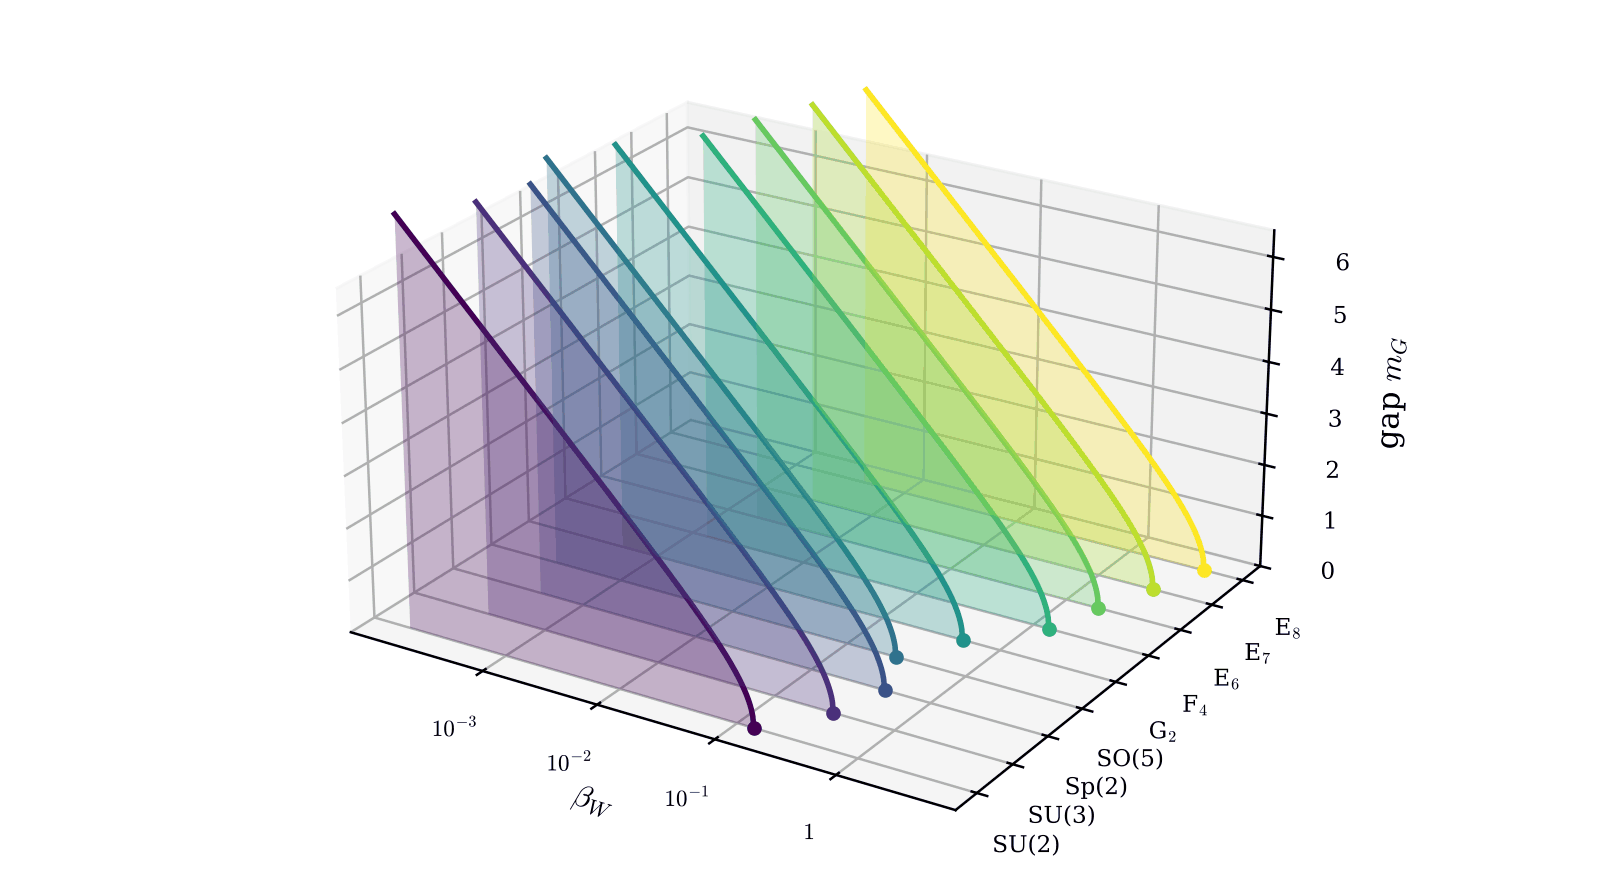
\includegraphics[width=0.9\textwidth]{figures/fig_groups.png}
\caption{The gap $m_G(\beta)$ of Theorem~\ref{thm:groups} as a function of
$\beta_W=N^2\beta$ on a logarithmic scale, for nine groups in the
representations of Table~\ref{tab:groups}. Each curve ends at the edge
$\beta_W=2N\kappa_G/29$ of the range, marked by a dot, where the gap tends to
zero; as $\beta_W\to0$ it grows like $\log(\kappa_G/(6N|\beta|))$. The
curves differ only by the factor $N\kappa_G$, since $m_G$ depends on
$N|\beta|/\kappa_G$ alone.}
\label{fig:groups}
\end{figure*}

No Bakry--\'Emery argument for the ungauged measure can pass $|\beta|=
\frac1{32}$~\cite[Thm.~C]{BB26a}; the gauge fixing changes the measure, not
the metric, which is why it can. For $\SU(2)$ the curvature range
$\beta_W<\frac4{29}$ lies inside that of Theorem~\ref{thm:su2}, and no
curvature argument for the gauge-fixed $\SU(2)$ measure passes
$\beta_W=\frac13$: when one active link $e$ is $-1$ and all others are $1$,
the six plaquettes through $e$ have variable $-1$, and along a geodesic
through $Q_e$ the Hessian of $-\frac{\beta_W}2\sum_p\ReTr Q_p$ is $-6\beta_W$
times the metric of the unit sphere $S^3$, whose Ricci curvature is $2$, so
the Bakry--\'Emery tensor is negative there once $\beta_W>\frac13$. For $\SU(3)$
the Dobrushin route goes much further.

\begin{theorem}[$\SU(3)$]\label{thm:su3}
Let $G=\SU(3)$ and $0\le\beta_W\le\frac34$. Then the conclusions
of Theorem~\ref{thm:su2} hold, with decay at every rate below
$-\log(1.33319\,\beta_W)$ and a transfer-matrix gap
\[
m\ge-\log(1.33319\,\beta_W)>0 .
\]
\end{theorem}

The proof of Theorem~\ref{thm:su3} bounds the Kantorovich modulus of the
one-link measure $\nu_b(dU)\propto e^{\ReTr(Ub)}dU$ on $\SU(3)$ uniformly over
staple sums $b$. Its analytic part is a lower bound for the spectral gap of
$\nu_b$ through Bochner's formula with a cross term
(Lemma~\ref{lem:gap}), a corrector chosen box by box among
polynomials of degree two in the matrix entries (Lemma~\ref{lem:corrector}), the reduction of
$b$ to diagonal matrices (Lemma~\ref{lem:orbits}), the character expansion
of the moments of $\nu_b$ (Lemma~\ref{lem:characters}) and an interpolation
inequality on boxes of staple sums (Lemma~\ref{lem:boxes}). The remaining
step evaluates the resulting bound on $2341$ boxes with rigorous error bounds;
the theorem rests on that computation, which is described in full in
Sec.~\ref{ssec:cover} and Appendix~\ref{app:cover}.

The plaquette blocks of Theorem~\ref{thm:blocks} work for $\SU(3)$ as well.
They use the same modulus of the one-link measure, but only through the
three links of a block, so they need $\Lambda(2\beta_W)$ small and not
$2r\Lambda(r)<1$: near the end of Theorem~\ref{thm:su3} they give a much
larger gap, and they go past it.

\begin{theorem}[$\SU(3)$ with plaquette blocks]\label{thm:su3blocks}
Let $G=\SU(3)$ and $0\le\beta_W\le\frac{19}{25}=0.76$. Then
$\alpha_3(\beta_W)<1$ for the number of~\eqref{eq:blockconst3}, with
$\alpha_3(0.72)\le0.9182$, $\alpha_3(\frac34)\le0.9653$ and
$\alpha_3(0.76)\le0.99950$. The conclusions of Theorem~\ref{thm:su2} hold
with decay at every rate below $-\frac12\log\alpha_3(\beta_W)$ and a
transfer-matrix gap
\[
m\ge-\tfrac12\log\alpha_3(\beta_W)>0 ;
\]
at $\beta_W=\frac34$ this gives $m\ge0.0177$, against $1.1\cdot10^{-4}$ from
Theorem~\ref{thm:su3}, and at $\beta_W=0.76$, where Theorem~\ref{thm:su3}
no longer applies, $m\ge2.5\cdot10^{-4}$.
\end{theorem}

\begin{table}[t]
\caption{Explicit ranges of uniqueness, decay and a transfer-matrix gap for
four-dimensional lattice Yang--Mills theory. The first three rows hold for
the ungauged measure; the last three are the results of this paper.}
\label{tab:ranges}
\begin{ruledtabular}
\begin{tabular}{lll}
Method&$\SU(2)$, $\beta_W$&$\SU(3)$, $\beta_W$\\
\colrule
Curvature, Shen--Zhu--Zhu~\cite{SZZ23}&$<\frac1{12}$&$<\frac3{16}$\\
Curvature, sharp~\cite{BB26a}&$<\frac18$&$<\frac9{32}$\\
Dobrushin, sharp quarter~\cite{BB26a}&$<\frac29$&\\
Curvature, forest gauge&$<\frac4{29}$&$<\frac9{29}$\\
Dobrushin, forest gauge&$<\frac13$&$\le\frac34$\\
Plaquette blocks, forest gauge&$\le0.345$&$\le0.76$\\
\end{tabular}
\end{ruledtabular}
\end{table}

\begin{figure*}[t]
\centering
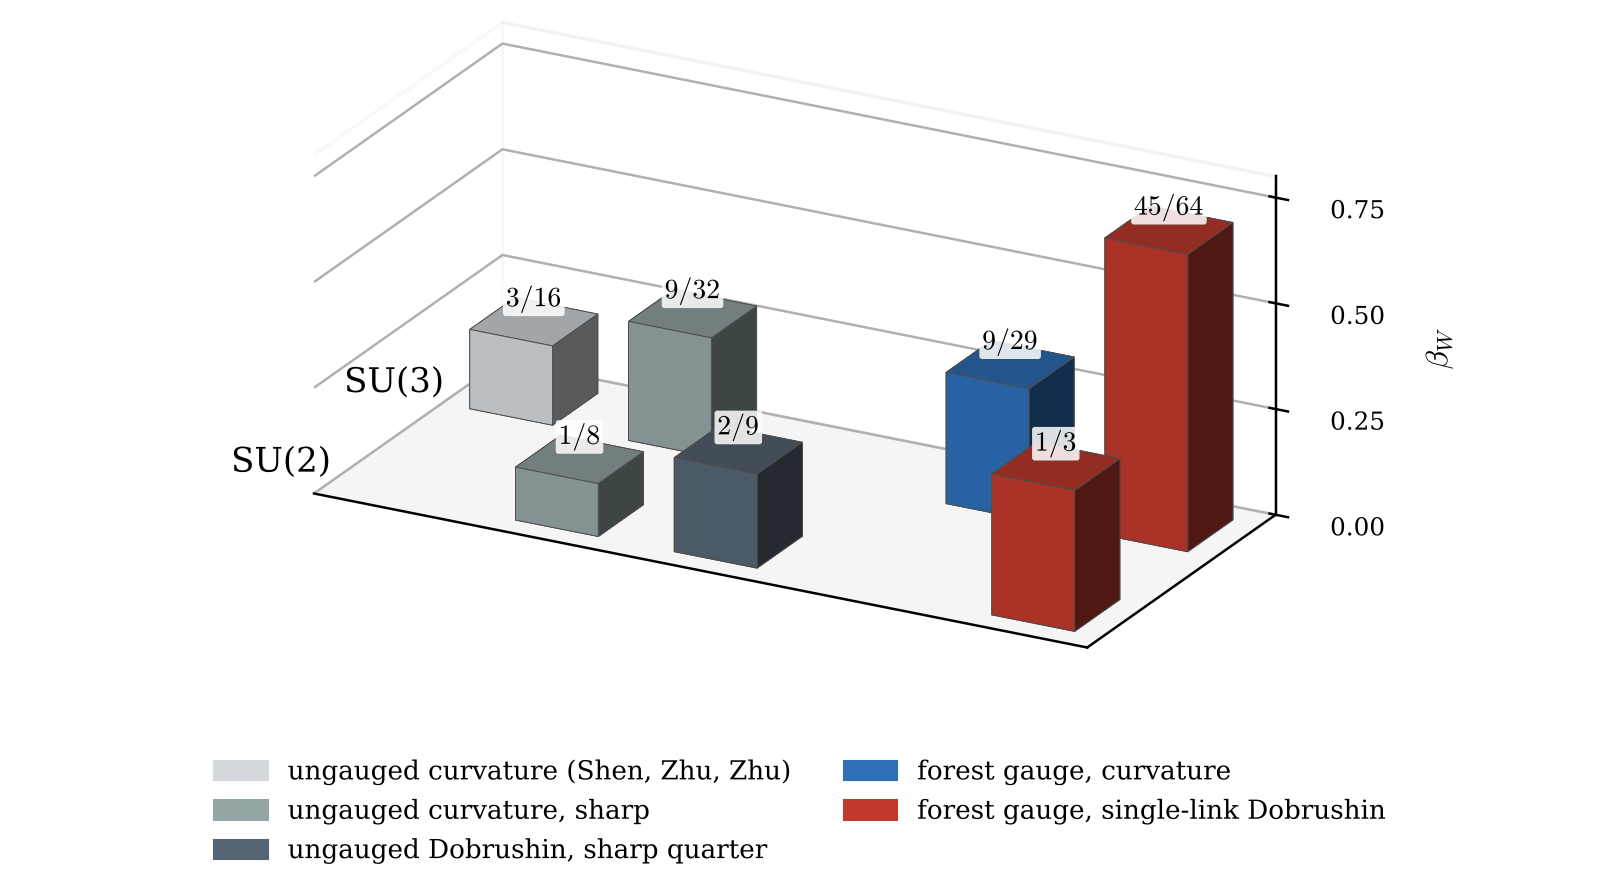
\includegraphics[width=0.86\textwidth]{figures/fig_ranges.png}
\caption{Ranges of Table~\ref{tab:ranges}. The height of each bar is the
largest inverse coupling $\beta_W$ covered by the method. Grey bars are
methods for the ungauged measure; blue, red and orange bars use the forest
gauge. For $\SU(2)$ the red bar ends at the ceiling of
Theorem~\ref{thm:ceiling} and the orange bar, plaquette blocks, passes it
(Theorem~\ref{thm:blocks}); for $\SU(3)$ the red bar is
Theorem~\ref{thm:su3} and the orange bar, plaquette blocks, gives a larger
gap there and passes it (Theorem~\ref{thm:su3blocks}).}
\label{fig:ranges}
\end{figure*}

All seven theorems are statements at fixed lattice spacing. They do not touch
the continuum limit, the crossover to Ba{\l}aban's regime, or a gap in
physical units, which together are the Clay problem; Sec.~\ref{sec:limits}
says where each method stops and what remains of the four open problems
of~\cite{BB26a}. The obstruction proved in~\cite{BB26b}, that a lattice gap
uniform in lattice units forces trivial continuum two-point functions,
applies to all of them.

\emph{The continuum step.} Sec.~\ref{sec:bypass} goes past that obstruction
in one respect, through three implications, each proved.
\begin{enumerate}[label=\textup{(I\arabic*)},leftmargin=*]
\item A Dobrushin--Shlosman condition on one cube of fixed physical size,
uniform along the continuum tuning, gives a mass gap in physical units for
every continuum limit (Theorems~\ref{thm:onescale} and~\ref{thm:transfer}),
and so does exponential decay with constants of the renormalised
correlations of a spanning set of observables
(Theorem~\ref{thm:clustering}); this holds also for observables smoothed by
the spatial gradient flow
(Proposition~\ref{prop:spatialflow}).
\item The flowed observables, renormalised by one condition at a single
physical separation, have reflection positive continuum limits along
subsequences, and such a limit is nontrivial exactly when one ratio of
lattice two-point functions stays away from zero
(Theorem~\ref{thm:flowlimit}); that ratio is bounded above and below by
ratios of correlations of one slice field at fixed physical separations
(Proposition~\ref{prop:sliceratio}).
\item Tree bounds on the truncated correlations give all the higher
Schwinger functions as reflection positive distributions, imply the ratio
bound, and carry the conditional mass gap to every polynomial in the
smeared fields (Theorem~\ref{thm:higher}); for a smooth packet they give the
ratio with an explicit rate and a reference vector of finite energy
(Proposition~\ref{prop:treeenergy}).
\end{enumerate}
\emph{What is open.} The inputs of (I1)--(I3), namely the cube condition
along the tuning, the slice ratio in four dimensions and the tree bounds,
are not proved, and so the nontrivial existence of the continuum limit and
the gap in physical units remain open. Figure~\ref{fig:logic} shows how the
proved statements, the implications and the open inputs fit together.

Sec.~\ref{sec:inputs} measures the open inputs. The cube condition holds
at strong coupling, fails at every fixed cube size at weak coupling, forces
the gauge-fixed variables to be disordered on the scale of the cube, and
cannot be reached from estimates on single lines of links; for $\SU(N)$ it
needs cubes of side at least of order $(\beta_W/\log\beta_W)^{1/4}$
(Propositions~\ref{prop:cubesize} and~\ref{prop:cubesizeN}). For a Gaussian
field it holds at a fixed physical scale when the field has a mass and fails
exactly, at every size, when it is massless (Proposition~\ref{prop:gauss});
it also fails for the quadratic approximation of the forest gauge itself
(Proposition~\ref{prop:gaussforest}), and of every gauge fixed on an
invariant forest with infinite trees (Proposition~\ref{prop:gaussevery}). The order-two cases of the tree bounds
force the lattice gap below a fixed multiple of the lattice spacing, so no
strong coupling expansion gives them (Proposition~\ref{prop:treecritical}).
The slice ratio holds in two dimensions, where it is the exact solution of
lattice gauge theory (Remark~\ref{rem:twodslice}), and fails for a field
whose mass is fixed in lattice units; for the free field, conditioning an
energy packet on averages over blocks leaves a fixed fraction of its ordinary
variance at every lattice spacing, so a reduction to block averages has to be
measured in the reflected norm (Proposition~\ref{prop:blockfree}).

\emph{Block averages.} Sec.~\ref{sec:blocks} poses the cube condition for
block averages in a gauge whose fixed links are trees inside blocks of side
two. Its quadratic approximation then holds at every coupling once the cube
is large (Theorem~\ref{thm:constrainedcube}), and integrating out one scale
reduces it to a cube condition for the averages, which carry the coarse
quadratic form at every scale up to a factor between $1$ and $256$ that does
not depend on the scale, with an exponentially decaying kernel whose
constants do not depend on the scale either, and the constrained cube
condition holds at every scale with one cube side
(Corollary~\ref{cor:compose}, Proposition~\ref{prop:effective},
Theorems~\ref{thm:effectiveupper}, \ref{thm:effectivelocal}
and~\ref{thm:constrainedscales}); the averages along the lines of the forest
gauge, by contrast, leave one class of lines invisible and fail at every size
(Proposition~\ref{prop:invisible}). For the group-valued links, the straight
path between block roots gives a coarse link whose fibres satisfy a
coercivity bound for every compact group and every field
(Theorem~\ref{thm:pathcoercive}), but this map does not compose across
scales (Proposition~\ref{prop:thinpath}), and for every compact connected group no continuous
covariant block map treats the positions of a block alike
(Proposition~\ref{prop:nomean}). A cut-off of Ba{\l}aban's averaging
operation is continuous, covariant and coercive for every field and agrees
with the block averages to first order; it breaks the symmetry only at large
fields, as it must, and its constants are those of one step
(Theorem~\ref{thm:cutoff}). On fields with values in a maximal torus whose
curvature stays small at every scale it composes, with the energy
nonincreasing and the thin paths contracted (Theorem~\ref{thm:torusscales}), and for every compact group it composes
on fields whose curvatures at the successive scales have a small sum
(Theorem~\ref{thm:smallscales}). Under the $\SU(2)$ Wilson measure the
plaquettes that are not small lie in clusters whose physical size tends to
zero in probability, and the cut-off acts only next to them
(Theorem~\ref{thm:defects}, Corollaries~\ref{cor:defectclusters}
and~\ref{cor:activelinks}); such plaquettes are nevertheless present along
the one-loop tuning (Proposition~\ref{prop:manydefects}). The cut-off
average composes through these clusters, which spread by at most three
spacings of the current scale per step, up to a coarse spacing of order
$(\beta_W/\log\beta_W)^{1/4}a$, the order of the cube side that the cube condition
needs
(Theorem~\ref{thm:defectscales} and Corollary~\ref{cor:defectscales}).
In a box whose boundary field has small plaquettes and either lies in a
maximal torus or, for $\SU(2)$, has plaquette angles $\rho_s$ with
$l^2\rho_s$ below a fixed constant, the fraction of unit cubes with a large
plaquette is small with probability exponentially close to one in the
volume, uniformly over such boundary fields
(Lemmas~\ref{lem:boxextension} and~\ref{lem:nonabelianfilling} and
Proposition~\ref{prop:conddensity}). The second class allows cube sides up
to a constant times $(\beta_W/\log\beta_W)^{1/4}$ at the level of
Corollary~\ref{cor:defectscales}, which is the scale $a_{k_*}$ up to a
constant factor; for larger boxes with general boundary fields this
conditional estimate is open (Remark~\ref{rem:boxnonabelian}).
On the fibres of the cut-off average, at a background whose plaquettes are
at most $\kappa\le10^{-8}$, the gap $\frac1{52}$ of the averages\footnote{By the certificate of
Proposition~\ref{prop:blockgapsharp} this gap is at least
$\frac{537}{5000}=0.1074$, within $0.09$ per cent of the best constant on $\Z^4$, a
floating-point value.}
persists up
to a factor $1+O(\kappa)$, and the Hessian of the action along the fibre is
at least $\lambda(\frac1{26}-c\kappa)$, however far the links are from $I$
(Theorem~\ref{thm:smallfibre}). On a chart of the fibre with convex domain
the constrained law is log-concave for large $\lambda$, coarea factor
included, and satisfies a Brascamp--Lieb inequality with constant
$60/\lambda$ (Theorem~\ref{thm:fibrechart}); on a chart whose domain is a
product in the coordinates of the links other than the path links, the
covariances of local observables decay exponentially at a rate that
depends only on $G$ (Theorem~\ref{thm:chartdecay}); its mass off the chart
is open (Remark~\ref{rem:chartdecayopen}).
Whether some block map is coercive for all fields and composes across the
remaining scales is open.

\begin{figure*}[t]
\centering
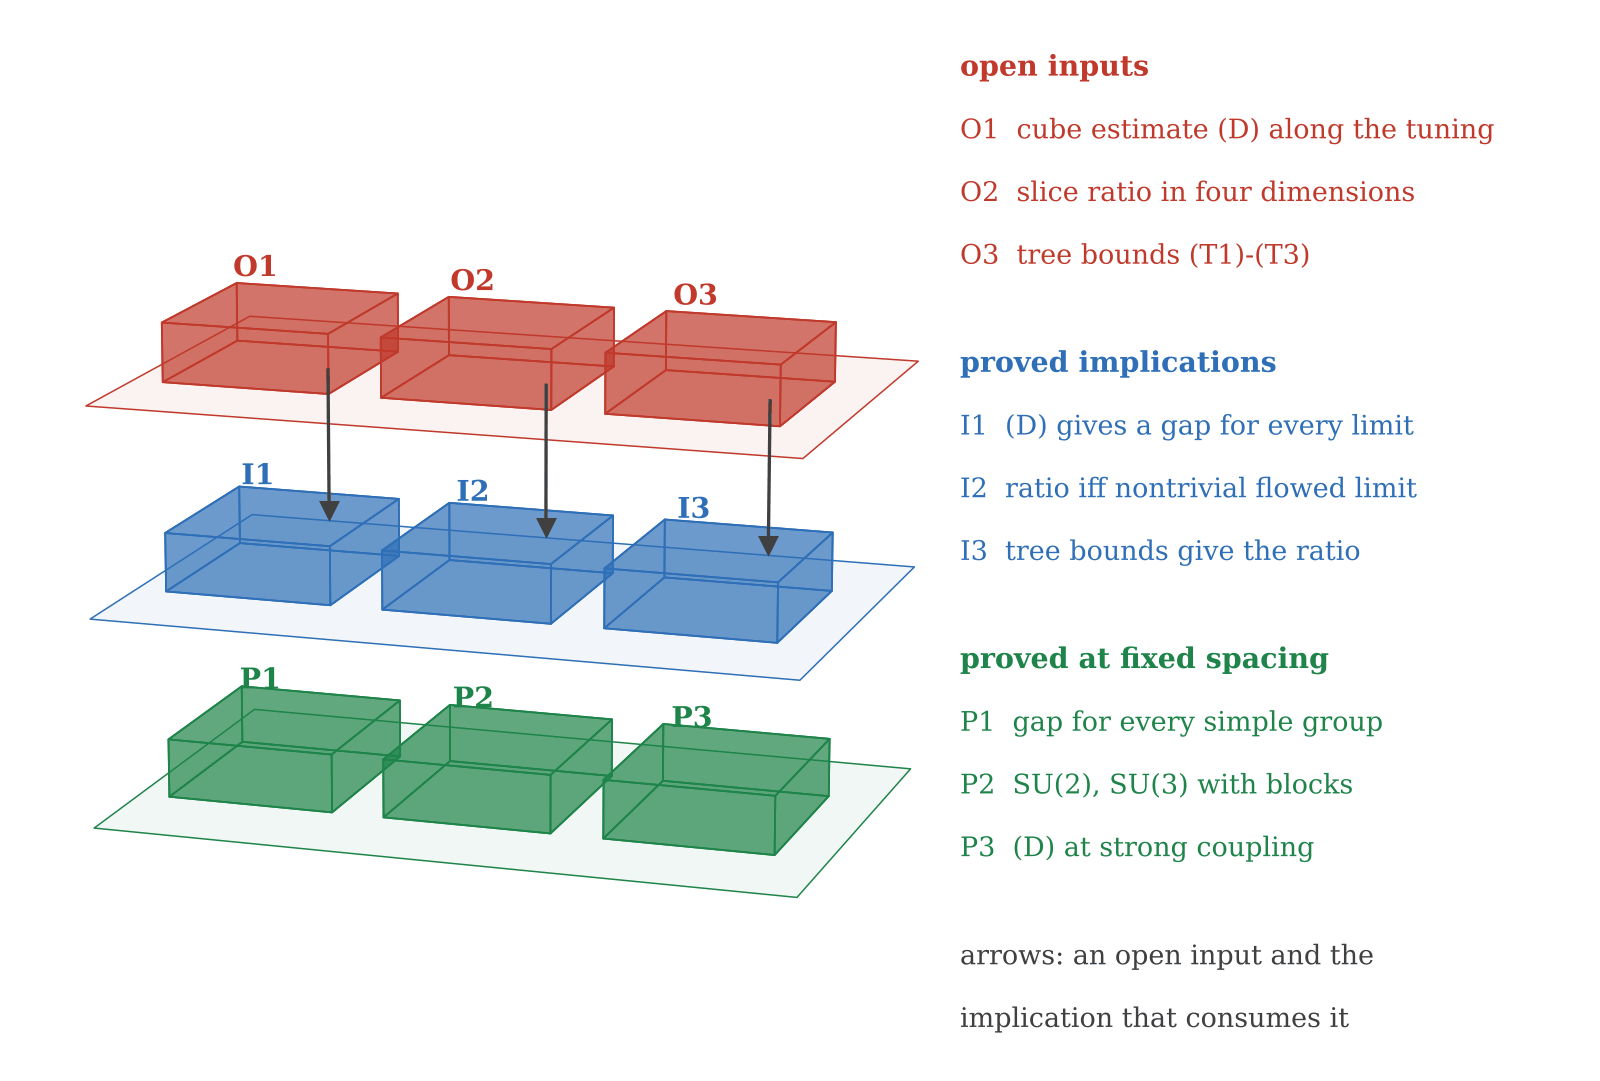
\includegraphics[width=0.9\textwidth]{figures/fig_logic.png}
\caption{The logical structure of the paper. Green: theorems at fixed
lattice spacing (P1 the gap for every compact simple group,
Theorem~\ref{thm:groups}, P2 the plaquette blocks for $\SU(2)$
and $\SU(3)$, P3 the cube condition at strong coupling). Blue: the proved
implications (I1)--(I3) of the continuum step. Red: their inputs, none of
which is proved along the continuum tuning. Each arrow joins an open input
to the implication that consumes it; no implication feeds its own input.}
\label{fig:logic}
\end{figure*}

\emph{Plan.} Sec.~\ref{sec:linefield} constructs the line field.
Sec.~\ref{sec:state} shows that a Dobrushin bound for the gauge-fixed
specification gives the full conclusion of Theorem~\ref{thm:su2}.
Secs.~\ref{sec:su2}, \ref{sec:plaqblocks}, \ref{sec:curvature},
\ref{sec:su3} and~\ref{sec:su3blocks} prove Theorems~\ref{thm:su2}--\ref{thm:su3blocks}, and
Sec.~\ref{sec:limits} measures what is left. Sec.~\ref{sec:bypass} proves
(I1)--(I3), Sec.~\ref{sec:inputs} states and measures their open inputs, and
Sec.~\ref{sec:blocks} poses the cube condition for block averages, composes the cut-off average
across scales at small fields and locates the large fields under the
Wilson measure. The appendices contain the
residue table of the line field, the comparison lemma and its version for
blocks, the blocks of the local Hessian inequality, the details of the
certified computation, the reconstruction of the transfer matrix with the
equivalence of a gap and exponential clustering
(Appendix~\ref{app:transfer}), the facts on spectral measures and on the
character expansion that the continuum step uses
(Appendices~\ref{app:spectral} and~\ref{app:characters}), and a complete
proof of the sharp quarter for the single-link law of $\SU(2)$
(Appendices~\ref{app:sharp}--\ref{app:bessel}), so that the paper does not
depend on our earlier one for any step.

\section{The line field}\label{sec:linefield}

Write $e_0,\dots,e_3$ for the unit vectors of $\Z^4$ and $(x,\mu)$ for the
link from $x$ to $x+e_\mu$. A \emph{direction field} is a map
$\sigma:\Z^4\to\{0,1,2,3\}$; its links are $F=\{(x,\sigma(x)):x\in\Z^4\}$. At
each site put $\pi_x(\mu)=\sigma(x+e_\mu)$. The plaquette at $x$ in the plane
$\{\mu,\nu\}$ has the links $(x,\mu)$, $(x+e_\mu,\nu)$, $(x+e_\nu,\mu)$,
$(x,\nu)$, so it contains
\begin{equation}\label{eq:count}
[\sigma(x)\in\{\mu,\nu\}]+[\pi_x(\mu)=\nu]+[\pi_x(\nu)=\mu]
\end{equation}
links of $F$.

\begin{lemma}\label{lem:cycle}
Every plaquette of $\Z^4$ contains exactly one link of $F$ if and only if, at
every site $x$, $\pi_x$ fixes $\sigma(x)$ and permutes the other three
directions cyclically.
\end{lemma}

\begin{proof}
Fix $x$, let $s=\sigma(x)$ and let $R$ be the set of the other three
directions. For a plane $\{s,\nu\}$ the count~\eqref{eq:count} is $1+[\pi_x(s)
=\nu]+[\pi_x(\nu)=s]$; it equals one for all $\nu\in R$ exactly when
$\pi_x(s)=s$ and $\pi_x(\nu)\ne s$ for $\nu\in R$, that is, when $\pi_x$ fixes
$s$ and maps $R$ into $R$. For a plane $\{\mu,\nu\}\subset R$ the count is
$[\pi_x(\mu)=\nu]+[\pi_x(\nu)=\mu]$. Draw an arrow $\mu\to\pi_x(\mu)$ for every
$\mu\in R$ with $\pi_x(\mu)\in R\setminus\{\mu\}$. Each vertex of $R$ has at most
one outgoing arrow, and the condition says that each of the three pairs of
$R$ carries exactly one arrow. Three arrows on three vertices with out-degree
at most one give out-degree exactly one everywhere, and a tournament on three
vertices with all out-degrees one is a directed three-cycle.
\end{proof}

From now on $\sigma$ is the field of period two given in
Table~\ref{tab:sigma} of Appendix~\ref{app:table}, read from $x$ modulo two.
The table lists $\pi_x$ at each of the sixteen residue classes; in each row
$\pi_x$ fixes $\sigma(x)$ and is a three-cycle on the rest, so every plaquette
contains exactly one link of $F$ by Lemma~\ref{lem:cycle}.\footnote{There are
exactly eight period-two direction fields with this property, all equivalent
to $\sigma$ under the symmetries of the lattice. A field with one fixed link
at every site and one in every plaquette exists only in four dimensions: a
link lies in $2(d-1)$ plaquettes and a site carries $d(d-1)/2$ of them, and
$2(d-1)=d(d-1)/2$ forces $d=4$. The statements of this section are also
checked in the Lean certificate of the archive.}

\begin{lemma}\label{lem:structure}
\begin{enumerate}[label=\textup{(\roman*)},leftmargin=*]
\item $F$ is a disjoint union of bi-infinite straight lines, one through
every site: every site has exactly one outgoing and one incoming link of $F$,
and both point in the direction $\sigma(x)$.
\item For every box $\Lambda$ (a product of four finite intervals, with the
links and plaquettes it contains), $F\cap E(\Lambda)$ is a disjoint union of
segments, hence a forest.
\item A link $e=(x,\mu)\notin F$ lies in six plaquettes. Four of them contain
a link of $F$ that shares an end point with $e$, and these lie in the planes
$\{\mu,\sigma(x)\}$ and $\{\mu,\pi_x(\mu)\}$. In the other two, which lie in
the remaining plane $\{\mu,\rho\}$, the link of $F$ is opposite to $e$.
\item Every link outside $F$ shares a plaquette with exactly twelve other
links outside $F$, two in each of its plaquettes.
\end{enumerate}
\end{lemma}

\begin{proof}
(i) Since $\pi_x$ fixes $\sigma(x)$, $\sigma(x+e_{\sigma(x)})=\sigma(x)$.
Because $\sigma$ has period two, $x-e_\mu\equiv x+e_\mu$, so also
$\sigma(x-e_{\sigma(x)})=\sigma(x)$, and the link $(x-e_{\sigma(x)},\sigma(x))$ is
in $F$. Conversely, if $(x-e_\nu,\nu)\in F$, then $\sigma(x-e_\nu)=\nu$, and
straightness at $x-e_\nu$ gives $\sigma(x)=\nu$. So the incoming link is unique
and continues the outgoing one.

(ii) A line meets a box in a segment, and distinct lines are disjoint.

(iii) The plaquettes of $e$ are, for each $\nu\ne\mu$, the one at $x$ and the
one at $x-e_\nu$ in the plane $\{\mu,\nu\}$. A link of $F$ sharing an end point
with $e$ is the outgoing or the incoming link of $F$ at $x$ or at $x+e_\mu$.
At $x$ both point in the direction $s=\sigma(x)\ne\mu$, and they lie in the
plaquettes at $x$ and at $x-e_s$ in the plane $\{\mu,s\}$. At $x+e_\mu$ both
point in the direction $t=\pi_x(\mu)$, which lies in $R\setminus\{\mu\}$ because
$\pi_x$ is a three-cycle on $R$, and they lie in the plaquettes at $x$ and at
$x-e_t$ in the plane $\{\mu,t\}$. These four plaquettes are distinct because
$s\ne t$. Each plaquette contains exactly one link of $F$, so in the two
plaquettes of the third plane $\{\mu,\rho\}$ the link of $F$ is a link of
direction $\mu$ or $\rho$ not touching $e$; the links of direction $\rho$ in
such a plaquette touch $e$, so it is the opposite link.

(iv) Each of the six plaquettes contains $e$, one link of $F$ and two other
links, and two distinct links share at most one plaquette.
\end{proof}

\begin{figure*}[t]
\centering
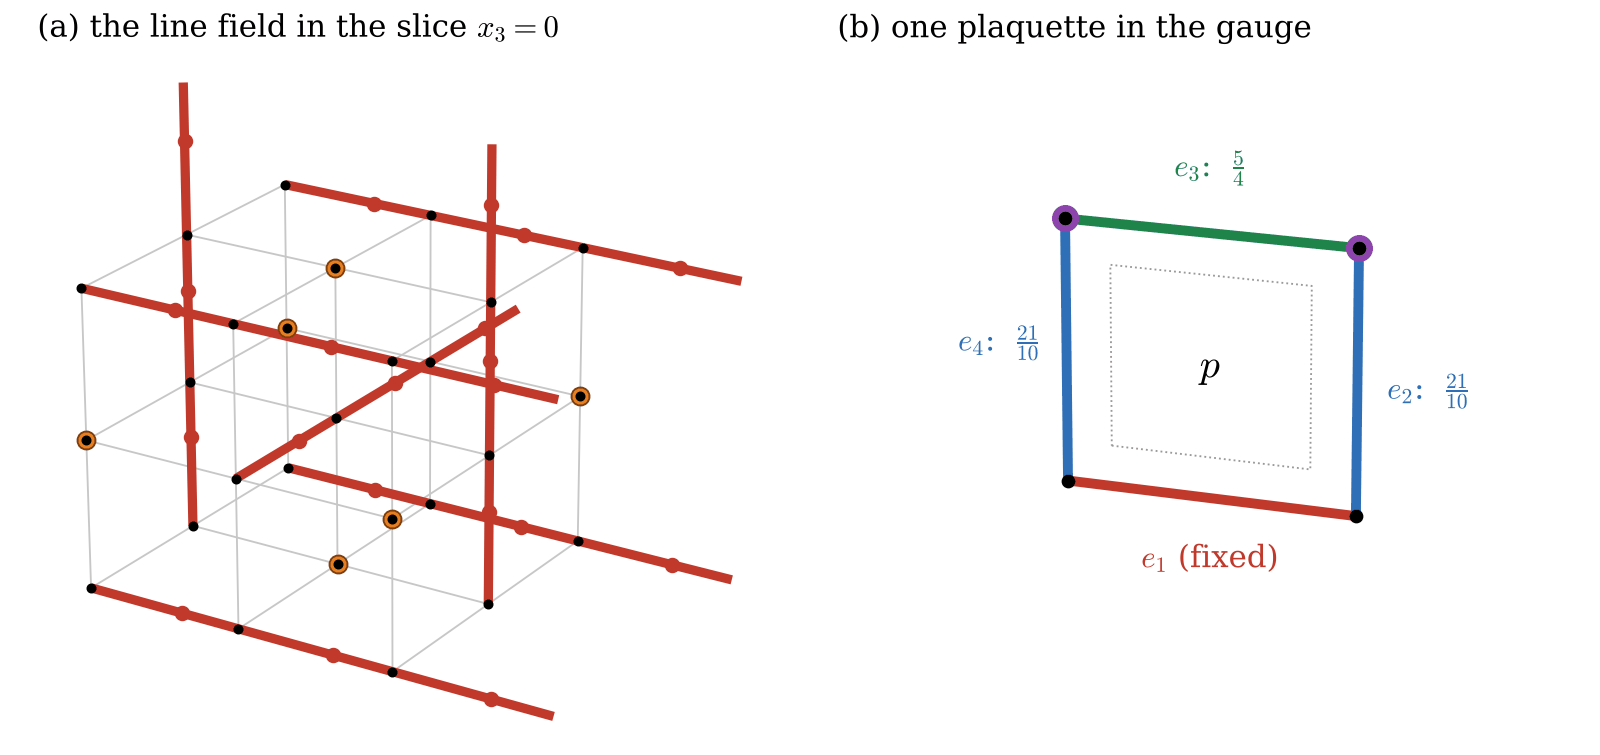
\includegraphics[width=0.9\textwidth]{figures/fig_linefield.png}
\caption{(a) The line field in the slice $x_3=0$ of a box of side three.
Thick red segments are the links of $F$ in the directions $0,1,2$, with a dot
marking the direction of travel; an orange ring marks a site whose line
leaves the slice in direction~$3$. Every line is straight
(Lemma~\ref{lem:structure}(i)), and the segments that leave the box are its
boundary stubs. (b) One plaquette with its fixed link $e_1$. The weights are
those of the local inequality of Lemma~\ref{lem:local} for the three free
links: $\frac{21}{10}$ on the two links adjacent to $e_1$ and $\frac54$ on the
opposite one. The two purple corners are the ones that enter the corner
form~\eqref{eq:corner} once $Y_1=0$.}
\label{fig:linefield}
\end{figure*}

\section{Gauge fixing and the free-boundary state}\label{sec:state}

Let $G\subset\U(N)$ be compact with Haar measure $dU$, and let $\Lambda$ be a
box. The Wilson measure with free boundary is
\[
W_\Lambda(dQ)=\frac1{Z_\Lambda}\exp\Bigl(N\beta\sum_{p\in P(\Lambda)}\ReTr
Q_p\Bigr)\prod_{e\in E(\Lambda)}dQ_e .
\]
The measure is invariant under the gauge transformations $Q_{(x,y)}\mapsto
g_xQ_{(x,y)}g_y^{-1}$ with $g\in G^\Lambda$. Call the links outside $F$ \emph{active} and
write $A$ for their set. For a function $O$ of the links, $O^F$ is $O$ with
every link of $F$ set to the identity.

\begin{lemma}[Gauge fixing]\label{lem:gaugefix}
Let $\mu^F_\Lambda$ be the probability measure on $G^{A\cap E(\Lambda)}$
whose density with respect to Haar measure is proportional to
$\exp(N\beta\sum_{p\in P(\Lambda)}\ReTr Q^F_p)$. For every gauge-invariant $O$ on $G^{E(\Lambda)}$,
\[
W_\Lambda(O)=\mu^F_\Lambda(O^F).
\]
\end{lemma}

\begin{proof}
Each segment of $F\cap E(\Lambda)$ is a path $x_0,x_1,\dots,x_k$ along one
direction. Given the variables on $F$, put $g_{x_0}=1$ and $g_{x_{i+1}}=
g_{x_i}Q_{(x_i,x_{i+1})}$ on every segment. The transformed field has $Q^g_e
=1$ on $F\cap E(\Lambda)$, and for fixed values on $F$ the map $Q_A\mapsto
Q^g_A$ is a product of left and right translations, which preserves Haar
measure. Gauge invariance of the action and of $O$ and the change of
variables give the claim.
\end{proof}

No leftover holonomy appears because $F\cap E(\Lambda)$ is a forest. The
measures $\mu^F_\Lambda$ are finite-volume versions of the specification
$\gamma^F$ on $G^A$: for $e\in A$, $\gamma^F_e$ resamples $Q_e$ from the law
with density proportional to $\exp(N\beta\sum_{p\ni e}\ReTr Q^F_p)$ given all
other active links. No infinite-volume gauge transformation is performed;
$\gamma^F$ is a specification in its own right. Fix a metric $\delta$ on $G$
of diameter $D$ that is bi-invariant (for $\SU(2)$ the chordal metric on
$S^3$, $D=2$; for $\SU(N)$ the Hilbert--Schmidt distance). The Kantorovich
coefficient of $e'$ on $e$ is
\[
C_{ee'}=\sup\frac{W_1\bigl(\gamma^F_e(\cdot\mid Q),\gamma^F_e(\cdot\mid
Q')\bigr)}{\delta(Q_{e'},Q'_{e'})},
\]
the supremum over pairs of configurations that differ only at $e'$. It
vanishes unless $e$ and $e'$ share a plaquette.

\begin{proposition}\label{prop:state}
Suppose that every row and every column of $(C_{ee'})$ sums to at most
$\alpha<1$. Then:
\begin{enumerate}[label=\textup{(\roman*)},leftmargin=*]
\item $\gamma^F$ has exactly one Gibbs measure $\mu_F$;
\item for every gauge-invariant local $O$ the limit $\omega(O)=\lim
W_\Lambda(O)$ exists along every sequence of boxes exhausting $\Z^4$ and
equals $\mu_F(O^F)$;
\item $\omega$ is invariant under translations and the hypercubic group;
\item if $\beta\ge0$, $\omega$ is reflection positive for reflections in
hyperplanes through sites and in hyperplanes bisecting links;
\item for gauge-invariant local $O,O'$ with $O$ Lipschitz in each link,
$|\Cov_\omega(O,O')|\le C_{O,O'}e^{-\lambda\dist(O,O')}$ for every
$\lambda<-\log\alpha$;
\item if $\beta\ge0$, the transfer matrix of $\omega$ has spectral gap at
least $-\log\alpha$.
\end{enumerate}
\end{proposition}

\begin{proof}
(i) Gibbs measures exist by compactness, and the comparison lemma of
Appendix~\ref{app:comparison} with $S=\emptyset$ shows that any two coincide.

(ii) Extend $\mu^F_\Lambda$ by Haar measure on the active links outside
$\Lambda$, and let $S$ be the set of active links with a plaquette outside
$P(\Lambda)$; this includes every active link outside $E(\Lambda)$. For an
active link $e\notin S$ all six plaquettes of $e$ lie in $P(\Lambda)$, so the
conditional law of $Q_e$ under the extended measure is $\gamma^F_e$. Let $T$
be the support of $O^F$ and $\lambda<-\log\alpha$. The comparison lemma with
weights $e^{-\lambda\dist(\cdot,T)}$ gives
\[
|\mu^F_\Lambda(O^F)-\mu_F(O^F)|\le L\,\frac{\theta D}{1-\theta}
\sum_{z\in S}e^{-\lambda\dist(z,T)},
\]
with $\theta=\alpha e^\lambda<1$ and $L$ a Lipschitz constant of $O^F$; the
sum is at most $C_TR^3e^{-\lambda R}$ when $R$ is the distance from $T$ to the
complement of $\Lambda$. For $O$ continuous but not Lipschitz, approximate
uniformly. Lemma~\ref{lem:gaugefix} gives $W_\Lambda(O)=\mu^F_\Lambda(O^F)$.

(iii) $W_\Lambda(\tau_vO)=W_{\Lambda-v}(O)$, and the boxes $\Lambda-v$ also
exhaust $\Z^4$; by (ii) the limit does not depend on the sequence. The line
field is a device for computing $W_\Lambda$ and is never shifted. The same
argument applies to the hypercubic group.

(iv) For $\beta\ge0$ the measure $W_\Lambda$ is reflection positive for every
box symmetric under the reflection~\cite{OSei78}, and reflection positivity
passes to the limit along such boxes, which is $\omega$ by (ii).

(v) $\Cov_\omega(O,O')=\Cov_{\mu_F}(O^F,O'^F)$, and setting the links of $F$
to the identity keeps the Lipschitz property. The bound is
Corollary~\ref{cor:decay}.

(vi) Let $\vartheta$ be a time reflection and $\tau_t$ a time translation.
For gauge-invariant local $O$ that are Lipschitz in each link, (v) gives
$|\omega(\vartheta(\bar O)\tau_tO)-|\omega(O)|^2|\le C_Oe^{-\lambda t}$. On
the support of $O$ these functions are dense in the gauge-invariant part of
$L^2(\omega)$: gauge-invariant functions are functions on the compact
quotient of $G^{E}$ by the gauge group, Lipschitz functions for the quotient
metric are dense in $L^2$ of every finite measure on it, and they lift to
gauge-invariant Lipschitz functions. By Proposition~\ref{prop:gapdecay} the spectrum
of the transfer matrix on the complement of the vacuum lies in
$[0,e^{-\lambda}]$, for every $\lambda<-\log\alpha$.
\end{proof}

The proposition replaces the torus limits and the uniqueness of the
ungauged Gibbs measure used in~\cite[Thm.~F]{BB26a} by the free-boundary
limit, which has all the properties the reconstruction of the transfer
matrix needs.\footnote{On a torus the line field closes up into cycles, and
the holonomies along them cannot be removed by a gauge transformation; the
argument never uses a torus. The state $\omega$ is defined only on
gauge-invariant observables, which is all that the Osterwalder--Schrader
reconstruction~\cite{OS73,OS75,OSei78} uses.}

\section{SU(2) up to one third}\label{sec:su2}

\begin{proof}[Proof of Theorem~\ref{thm:su2}]
Identify $\SU(2)$ with the unit quaternions and use the chordal metric. For an
active link $e$ and a plaquette $p\ni e$, the staple $s_p$ is the product of the
other three link variables in the order that makes $\operatorname{Re}(Q_es_p)
=\frac12\Tr Q_p$, with links of $F$ equal to one. Since $N\beta\ReTr Q_p=
4\beta\ip{Q_e}{\bar s_p}$ in $\R^4$, the conditional law of $Q_e$ is the von
Mises--Fisher law $\nu_b(dx)\propto e^{\ip xb}dx$ on $S^3$ with $b=4\beta
\sum_{p\ni e}\bar s_p$. Changing a partner $e'$ by $\delta$ in the chordal
metric changes one staple by an isometric image of that displacement, so $b$
moves by $4|\beta|\delta$, and the sharp quarter (Theorem~\ref{q-thm:quarter}),
$W_1(\nu_b,\nu_{b'})\le\frac14|b-b'|$, gives $C_{ee'}\le|\beta|$. By
Lemma~\ref{lem:structure}(iv) every row and column has twelve nonzero
entries, so $\alpha\le12|\beta|=3|\beta_W|$. Proposition~\ref{prop:state}
applies for $|\beta_W|<\frac13$.
\end{proof}

\begin{proof}[Proof of Theorem~\ref{thm:ceiling}]
For the line field, every staple of an active link contains two active
links, so the six staples can be chosen with sum zero while the staple
through a given partner $e'$ moves freely. At $b=0$ the derivative of $\nu_b$
in the direction $h$ has Kantorovich norm $\frac14|h|$ by Lemma~\ref{q-lem:rate}(i),
so $C_{ee'}=|\beta|$ exactly, and every row sum is $12|\beta|=3|\beta_W|$.

Now let $F'$ be any forest and $C'$ the matrix of the statement. Suppose a
positive weight $w$ satisfies $C'w\le\alpha w$. For a box $\Lambda_n$ of side
$n$ let $C_n$ be the principal submatrix on the active links of $E(\Lambda_n)$;
then $C_nw\le\alpha w$ on these links, and the Collatz--Wielandt inequality
for nonnegative matrices gives $\rho(C_n)\le\alpha$. Since $C_n$ is symmetric,
$\rho(C_n)$ is at least the mean row sum. The box has $4n^4-O(n^3)$ links and
$n^4$ sites, and a forest has fewer links than sites, so the number $a$ of
active links is at least $3n^4-O(n^3)$. Let $a_p$ be the number of active
links of the plaquette $p$; the box has $P=6n^4-O(n^3)$ plaquettes and
$\sum_pa_p=6a-O(n^3)$. Two links share at most one plaquette, so the row
sums add up to $|\beta|\sum_pa_p(a_p-1)$, and by convexity
\[
\frac{|\beta|}a\sum_pa_p(a_p-1)\ge\frac{|\beta|P}a\,\bar a(\bar a-1)
=6|\beta|(\bar a-1)-o(1),
\]
with $\bar a=\sum_pa_p/P=6a/P-o(1)\ge3-o(1)$. Hence $\alpha\ge12|\beta|-o(1)$
for every $n$, and $\alpha\ge12|\beta|=3|\beta_W|$.
\end{proof}

Without gauge fixing the same count gives eighteen partners and the ceiling
$\beta_W=\frac29$ of~\cite[Prop.~13]{BB26a}; the temporal gauge, a family of
lines in one direction, leaves fourteen. The line field is optimal among
forests: twelve is the mean number of partners forced by the number of free
links, and it is attained at every link.

\section{SU(2) past one third: plaquette blocks}\label{sec:plaqblocks}

Throughout this section $G=\SU(2)$ is the group of unit quaternions with
the chordal metric $|x-y|$, $\bar x$ is the conjugate, $\ip xy=\operatorname{Re}
(x\bar y)$ is the inner product of $\R^4$, and $dx$ is the normalised Haar
measure on $S^3$. Left and right multiplication by unit quaternions and
conjugation are isometries, and $\operatorname{Re}(xyz)=\operatorname{Re}
(yzx)=\ip y{\bar z\bar x}$. Put
\[
Z_0(c)=\int_{S^3}e^{\ip cx}dx=\sum_{j\ge0}\frac{(|c|^2/4)^j}{j!\,(j+1)!},
\qquad c\in\R^4,
\]
let $\nu_c(dx)\propto e^{\ip cx}dx$ be the von Mises--Fisher law, and write
$g=\log Z_0$, so that $\nabla g(c)$ is the mean and $\Hess g(c)$ the
covariance of $\nu_c$.

\subsection{The blocks}

Let $\mathcal B$ be the set of plaquettes at $x$ in the plane $\{0,1\}$ with
$x_0\equiv x_1$ and in the plane $\{2,3\}$ with $x_2\equiv x_3$, congruences
modulo two (Table~\ref{tab:plaqblocks} of Appendix~\ref{app:plaqblocks} lists
them modulo $2\Z^4$, and Fig.~\ref{fig:plaqblocks} draws them). A
\emph{block plaquette} is a plaquette of $\mathcal B$, and its \emph{block}
is the set of its three active links.

\begin{lemma}\label{lem:plaqblocks}
The set $\mathcal B$ is invariant under translations by $2\Z^4$ and:
\begin{enumerate}[label=\textup{(\roman*)},leftmargin=*]
\item the blocks partition the active links;
\item every plaquette $p\notin\mathcal B$ meets three distinct blocks, one in
each of its active links;
\item every active link lies in exactly five plaquettes outside $\mathcal B$,
so it shares a plaquette outside $\mathcal B$ with exactly ten active links,
none of them in its own block;
\item if an active link $j$ and a link of a block $B$ lie in a common
plaquette outside $\mathcal B$, then every link of $B$ has its midpoint
within distance $2$ of the midpoint of $j$.
\end{enumerate}
\end{lemma}

\begin{proof}
Invariance under $2\Z^4$ is clear from the congruences. We use one fact
throughout: two distinct links lie in at most one common plaquette, since
they span it.

Every link lies in exactly one plaquette of $\mathcal B$. Indeed, a link
$(y,\mu)$ with $\mu\in\{0,1\}$ lies in no plaquette of the plane $\{2,3\}$,
and in exactly two of the plane $\{0,1\}$, those at $y$ and at $y-e_\nu$,
where $\nu$ is the other element of $\{0,1\}$. The base points $y$ and
$y-e_\nu$ differ only in the coordinate $\nu$, so $y_0-y_1$ has opposite
parities at the two, and exactly one of them satisfies $x_0\equiv x_1$. The
directions $2,3$ are treated in the same way. Every plaquette of $\Z^4$
contains exactly one link of $F$ (Lemma~\ref{lem:cycle}), so a block
plaquette contains three active links, and every active link lies in exactly
one block. This is (i).

(ii) Let $p\notin\mathcal B$ have active links $e_1,e_2,e_3$, and let $q_i$ be
the block plaquette of $e_i$. Then $q_i\ne p$, so $q_i\cap p=\{e_i\}$ by the
fact above. If $q_i=q_k$ with $i\ne k$, then $e_i,e_k$ lie in the two
distinct plaquettes $p$ and $q_i$, which is impossible. So the three blocks are
distinct, and each meets $p$ in one link.

(iii) An active link $e$ lies in six plaquettes (Lemma~\ref{lem:structure}), and
by (i) exactly one of them is in $\mathcal B$. Each of the other five
contains two further active links. These ten links are distinct, because a
link other than $e$ shares at most one plaquette with $e$, and none lies in
the block of $e$, because a link $f$ of that block sharing the
plaquette $p\notin\mathcal B$ with $e$ would put $e,f$ in the two distinct
plaquettes $p$ and the block plaquette of $e$.

(iv) Let $f\in B$ share the plaquette $p\notin\mathcal B$ with $j$. Two links
of one unit square have midpoints at distance $2^{-1/2}$ or $1$, so the
midpoint of $j$ is within distance $1$ of that of $f$, and the midpoint of
$f$ is within distance $1$ of that of every link of its block plaquette. The
triangle inequality gives the bound $2$.
\end{proof}

\begin{figure*}[t]
\centering
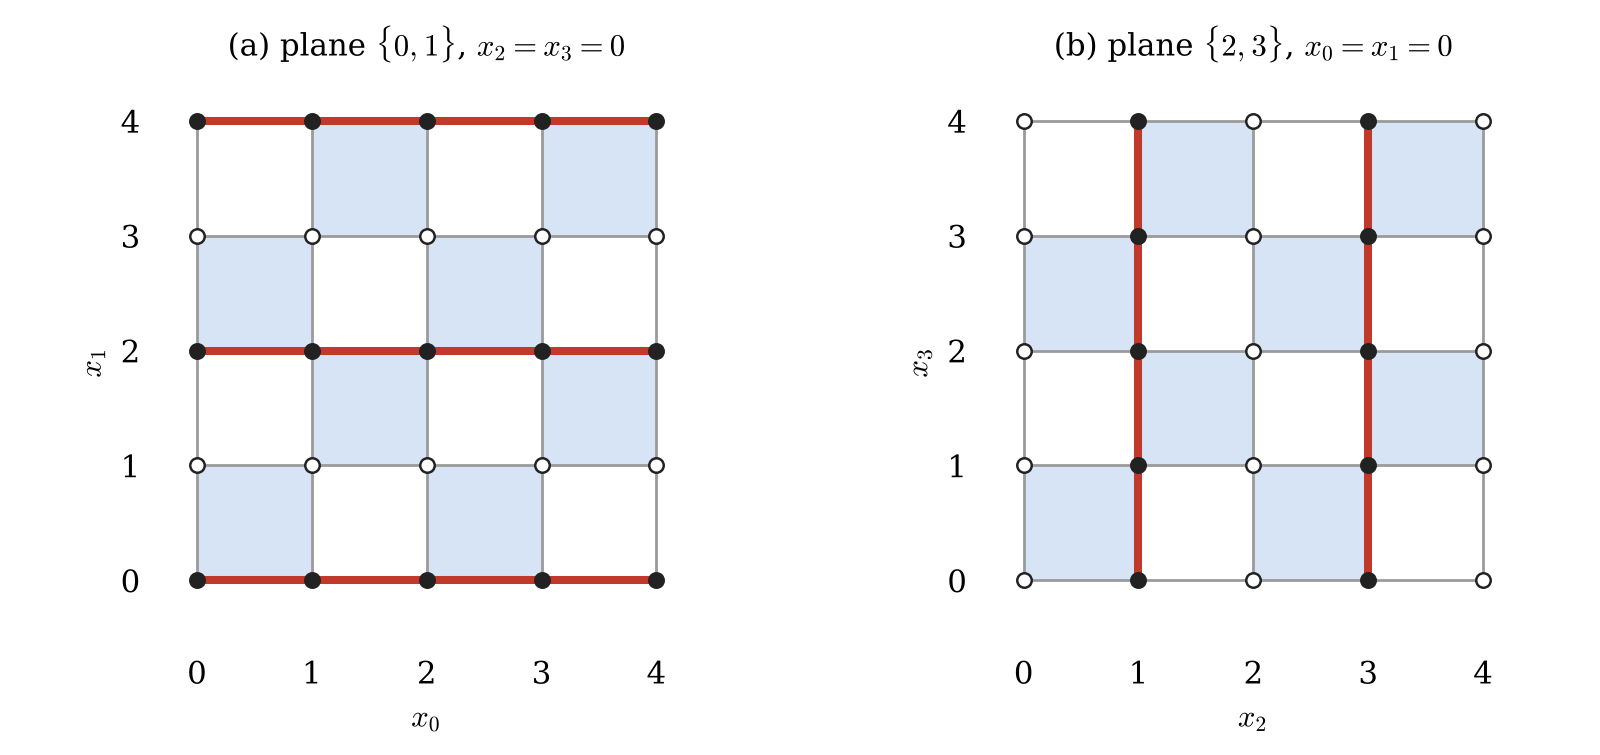
\includegraphics[width=0.82\textwidth]{figures/fig_plaqblocks.png}
\caption{Block plaquettes, shaded, in (a) a plane $\{0,1\}$ and (b) a plane
$\{2,3\}$: the plaquettes at $x$ with $x_0\equiv x_1$, respectively
$x_2\equiv x_3$, modulo two. Red links belong to the line field $F$; a filled
dot marks a site whose line runs in the plane, an open dot one whose line
leaves it. The shaded squares form a checkerboard, so every link of the plane
borders exactly one of them, and every square contains exactly one red link
(Lemma~\ref{lem:cycle}); hence each block plaquette carries three active
links and the blocks partition the active links
(Lemma~\ref{lem:plaqblocks}(i)).}
\label{fig:plaqblocks}
\end{figure*}

Fix a block plaquette $p$ with active links $e_1,e_2,e_3$. Reading the
plaquette product cyclically and deleting its fixed link, $\frac12\Tr Q_p=
\operatorname{Re}(y_1y_2y_3)$, where $y_i$ is $Q_{e_i}$ or $Q_{e_i}^{-1}$.
Every other plaquette containing $e_i$ meets the block only in $e_i$ by
Lemma~\ref{lem:plaqblocks}(ii) and contributes $4\beta\ip{y_i}{\bar s}$ to
the exponent, where $s$ is the staple of $y_i$ in it. Hence the conditional
law of the block given all other active links is
\begin{equation}\label{eq:blocklaw}
\mu_b(dy)\propto\exp\Bigl(\sum_{i=1}^3\ip{y_i}{b_i}+4\beta\operatorname{Re}
(y_1y_2y_3)\Bigr)dy_1\,dy_2\,dy_3,
\end{equation}
with $b_i$ the sum of $4\beta\bar s$ over the five staples, so that
$|b_i|\le20|\beta|$. Inversion is an isometry of $S^3$ and preserves Haar
measure, so we may work with $y$ instead of $Q$. On $(S^3)^3$ we use the
metric $d(y,y')=\sum_i|y_i-y'_i|$.

\subsection{The sensitivity of one block}

Let $\lambda_*$ and $\tau$ be a lower and an upper bound for the
eigenvalues of $\Hess g(c)$ on the ball $|c|\le24|\beta|$, and $M$ an upper
bound there for the norm of the third derivative $D^3g(c)$ as a trilinear
form. Put
\begin{equation}\label{eq:blockconst}
\begin{gathered}
w=8\beta^2(\tau-\lambda_*),\qquad s=\tfrac14+(e^w-1)e^w\sqrt\tau,\\
C=20|\beta|\bigl(4|\beta|\tau s+16\beta^2M\bigr),\qquad
K=\frac{(1+|\beta|)\,s}{1-C},
\end{gathered}
\end{equation}
assuming $C<1$.

\begin{lemma}\label{lem:tilt}
Let $\nu$ be a probability measure and $\lambda=e^R\nu/\nu(e^R)$ with
$\operatorname{osc}R\le\omega$. For bounded $f,h$,
\[
\Cov_\lambda(f,h)\le\Cov_\nu(f,h)+(e^\omega-1)e^\omega\,\mathrm{sd}_\nu(f)
\,\mathrm{sd}_\nu(h).
\]
\end{lemma}

\begin{proof}
We may assume $0\le R\le\omega$. The density $\rho=e^R/\nu(e^R)$ lies in
$[e^{-\omega},e^\omega]$, so $\delta=\|\rho-1\|_\infty\le e^\omega-1$. With
$\tilde f=f-\nu f$ and $\tilde h=h-\nu h$,
\[
\begin{split}
\Cov_\lambda(f,h)-\Cov_\nu(f,h)={}&\nu\bigl((\rho-1)\tilde f\tilde h\bigr)\\
&-\nu\bigl((\rho-1)\tilde f\bigr)\,\nu\bigl((\rho-1)\tilde h\bigr),
\end{split}
\]
and the right side is at most $(\delta+\delta^2)\,\mathrm{sd}_\nu(f)\,
\mathrm{sd}_\nu(h)$ by the Cauchy--Schwarz inequality.
\end{proof}

\begin{lemma}\label{lem:onesite}
Let $\beta\ge0$, $a,c_0\in\R^4$ with $|a|,|c_0|\le20\beta$, and
\[
\kappa(dx)\propto\exp\bigl(\ip xa+g(c_0+4\beta\bar x)\bigr)dx
\quad\text{on }S^3 .
\]
For every $1$-Lipschitz $f$ and every $h\in\R^4$:
\begin{enumerate}[label=\textup{(\roman*)},leftmargin=*]
\item $\Cov_\kappa(f,\ip xh)\le s|h|$;
\item if $c_0$ moves in the direction $k$, then $|\frac{d}{dt}\kappa(f)|\le
(4\beta\tau s+16\beta^2M)|k|$.
\end{enumerate}
\end{lemma}

\begin{proof}
(i) Taylor's formula at $c_0$ gives $g(c_0+4\beta u)=g(c_0)+4\beta\ip{\nabla
g(c_0)}u+R(u)$ with $R(u)=8\beta^2\Hess g(\xi)(u,u)$ for some $\xi$ on the
segment, $|\xi|\le24\beta$. For $u=\bar x$ of norm one, $R(\bar x)\in[8\beta^2
\lambda_*,8\beta^2\tau]$, so $\operatorname{osc}R\le w$. Since $\ip{\nabla
g(c_0)}{\bar x}=\ip x{\overline{\nabla g(c_0)}}$, $\kappa$ is the tilt
$e^{R}\nu/\nu(e^R)$ of $\nu=\nu_c$ with $c=a+4\beta\overline{\nabla g(c_0)}$.
The sharp quarter, Theorem~\ref{q-thm:quarter}, gives $\Cov_\nu(f,\ip xh)=\frac{d}{dt}
\nu_{c+th}(f)\le\frac14|h|$. A $1$-Lipschitz function on a set of diameter
two has $\mathrm{sd}\le1$, and $\mathrm{sd}_\nu\ip xh\le\sqrt\tau|h|$
because $|c|\le|a|+4\beta\le24\beta$. Lemma~\ref{lem:tilt} gives (i).

(ii) The derivative is $\Cov_\kappa(f,\ip{\nabla g(c_0+4\beta\bar x)}k)$.
Write $\nabla g(c_0+4\beta u)=\nabla g(c_0)+4\beta\Hess g(c_0)u+N(u)$. The
constant term does not contribute. The linear term is $\ip xh$ with
$h=4\beta\,\overline{\Hess g(c_0)k}$, $|h|\le4\beta\tau|k|$, and contributes at
most $4\beta\tau s|k|$ by (i). For $|u|,|u'|\le1$, $\|\Hess g(c_0+4\beta v)-
\Hess g(c_0)\|\le4\beta M|v|\le4\beta M$ on the segment between them, so
$|N(u)-N(u')|\le16\beta^2M|u-u'|$; the function $\ip{N(\bar x)}k$ is
therefore $16\beta^2M|k|$-Lipschitz, its standard deviation is at most that
constant, and its covariance with $f$ is at most $16\beta^2M|k|$.
\end{proof}

\begin{lemma}\label{lem:blockK}
Let $C<1$. If $b$ and $b'$ satisfy $|b_i|,|b'_i|\le20|\beta|$ and differ
only in one coordinate $b_i$, then
\[
W_1(\mu_b,\mu_{b'})\le K\,|b_i-b'_i|
\]
in the metric $d$.
\end{lemma}

\begin{proof}
The map $y_1\mapsto-y_1$ turns $\mu_b$ for $\beta$ into the law for $-\beta$
with $b_1$ replaced by $-b_1$ and is an isometry, so we may take $\beta\ge0$;
the cyclic symmetry of $\operatorname{Re}(y_1y_2y_3)$ lets us take $i=1$. Let
$f$ be $1$-Lipschitz for $d$ and $\varepsilon=|b_1-b'_1|$.

\emph{The middle link.} Given $y_1,y_3$, the law of $y_2$ is $\nu_c$ with $c=
b_2+4\beta\,\overline{y_3y_1}$, which does not involve $b_1$. Changing $y_1$
by $\eta$ moves $c$ by $4\beta\eta$, and the sharp quarter moves $\nu_c$ by at
most $\beta\eta$ in $W_1$. Hence $F(y_1,y_3)=\E[f\mid y_1,y_3]$ is
$(1+\beta)$-Lipschitz in each variable, and $\mu_b(f)=\mu^{13}_b(F)$, where
$\mu^{13}_b$ is the law of $(y_1,y_3)$:
\[
\mu^{13}_b\propto e^{\ip{y_1}{b_1}+\ip{y_3}{b_3}}Z_0\bigl(b_2+4\beta\,
\overline{y_3y_1}\bigr).
\]
Since $|b_2+4\beta\overline{y_3y_1}|=|b_2y_3+4\beta\bar y_1|=|y_1b_2+
4\beta\bar y_3|$, its conditional laws are
\[
\begin{split}
\kappa_1(dy_1\mid y_3)&\propto e^{\ip{y_1}{b_1}+g(b_2y_3+4\beta\bar y_1)}dy_1,\\
\kappa_3(dy_3\mid y_1)&\propto e^{\ip{y_3}{b_3}+g(y_1b_2+4\beta\bar y_3)}dy_3,
\end{split}
\]
both of the form of Lemma~\ref{lem:onesite}, with $|c_0|=|b_2|$.

\emph{Two sites.} Integrating Lemma~\ref{lem:onesite}(i) along the segment
from $b_1$ to $b'_1$ gives $W_1(\kappa_1,\kappa'_1)\le s\varepsilon$ for the
same $y_3$. Moving $y_3$ to $y'_3$ moves $c_0=b_2y_3$ along a segment of
length $|b_2||y_3-y'_3|\le20\beta|y_3-y'_3|$ inside the ball $|c_0|\le20\beta$,
so Lemma~\ref{lem:onesite}(ii) gives $W_1(\kappa_1(\cdot\mid y_3),\kappa_1(
\cdot\mid y'_3))\le C|y_3-y'_3|$, and the same for $\kappa_3$, which does not
depend on $b_1$. Let $\pi$ be a coupling of $\mu^{13}_b$ and $\mu^{13}_{b'}$
minimising $d_1+d_3$, $d_k=\E_\pi|y_k-y'_k|$. Replacing $(y_1,y'_1)$ by an
optimal coupling of $\kappa_1(\cdot\mid y_3)$ and $\kappa'_1(\cdot\mid y'_3)$
keeps a coupling, so minimality gives $d_1\le s\varepsilon+Cd_3$; in the
same way $d_3\le Cd_1$. Hence $d_1\le s\varepsilon/(1-C^2)$ and
\[
|\mu_b(f)-\mu_{b'}(f)|\le(1+\beta)(d_1+d_3)\le\frac{(1+\beta)s}{1-C}
\,\varepsilon=K\varepsilon .\qedhere
\]
\end{proof}

\subsection{The constants}

\begin{lemma}\label{lem:vmfconst}
Write $g(c)=\varphi(|c|^2)$ and $r=|c|$. For $c\ne0$ the eigenvalues of
$\Hess g(c)$ are $2\varphi'(r^2)$, three times, and $2\varphi'(r^2)+4r^2
\varphi''(r^2)$, and the norm of $D^3g(c)$ is
\[
\max\Bigl(|A+\Gamma|,\tfrac23|A|\Bigr),\qquad A=12r\varphi''(r^2),\quad
\Gamma=8r^3\varphi'''(r^2).
\]
On the ball $r\le2.07$ every eigenvalue of $\Hess g$ lies between
$0.158491$ and $0.25000001$, and the norm of $D^3g$ is at most $0.0615586$.
\end{lemma}

\begin{proof}
Differentiating $\varphi(|c|^2)$ gives $D^2g(v,v)=2\varphi'|v|^2+4\varphi''
\ip cv^2$ and $D^3g(v,v,v)=12\varphi''\ip cv|v|^2+8\varphi'''\ip cv^3$. For
$|v|=1$ and $t=\ip{c/r}v\in[-1,1]$ the cubic form is $At+\Gamma t^3$, whose
largest absolute value is attained at $t=\pm1$ or at an interior critical
point, where it equals $\frac23|A||t|\le\frac23|A|$; by Banach's
theorem~\cite{Ban38} the supremum of a symmetric trilinear form on the
diagonal of the unit sphere is its norm. The numerical bounds are obtained
in ball arithmetic~\cite{Joh17} from the series of $Z_0$, truncated after
forty terms with a proved bound on the tail, on $2\cdot10^4$ subintervals of
$[0,2.07]$; the program is described in Appendix~\ref{app:plaqblocks}.
\end{proof}

\subsection{The proof of Theorem~\ref{thm:blocks}}

Let $\gamma^{\mathcal B}$ be the block specification: for a block $B$,
$\gamma^{\mathcal B}_B$ resamples the three links of $B$ from~\eqref{eq:blocklaw}.
It comes from the same interaction as $\gamma^F$, so the two specifications
have the same Gibbs measures. Define the block coefficients
\[
C_{Bj}=\sup\frac{W_1\bigl(\gamma^{\mathcal B}_B(\cdot\mid Q),\gamma^{\mathcal B}_B
(\cdot\mid Q')\bigr)}{|Q_j-Q'_j|}
\]
for an active link $j\notin B$, the supremum over pairs of configurations
that differ only at $j$, with $W_1$ for the metric $d$.

\begin{proposition}\label{prop:blockstate}
Suppose that $\sum_BC_{Bj}\le\alpha<1$ for every active link $j$. Then the
conclusions (i)--(vi) of Proposition~\ref{prop:state} hold with
$-\frac12\log\alpha$ in place of $-\log\alpha$.
\end{proposition}

\begin{proof}
The proof of Proposition~\ref{prop:state} goes through with
Lemma~\ref{lem:blockcomparison} of Appendix~\ref{app:comparison} in place of
Lemma~\ref{lem:comparison}, and with the set $S$ of part~(ii), and the
support of $H$ in Corollary~\ref{cor:decay}, enlarged to the union of the
blocks that meet it. The enlargement multiplies the size of these sets by at
most three and moves them by at most one, which changes only the constants.
\end{proof}

\begin{proof}[Proof of Theorem~\ref{thm:blocks}]
Let $|\beta|\le0.345/4$ and take the constants of Lemma~\ref{lem:vmfconst},
whose ball $r\le2.07$ contains $|c|\le24|\beta|$. With these fixed constants
every quantity in~\eqref{eq:blockconst} is increasing in $|\beta|$, and so is
\begin{equation}\label{eq:alphablock}
\alpha(\beta_W)=40|\beta|K .
\end{equation}
Changing an active link $j$ by $\eta$ changes one staple of each of its ten
partners outside its block by an isometric image of the displacement, so the
field $b_i$ of each such partner $i$ moves by at most $4|\beta|\eta$, and
Lemma~\ref{lem:blockK}, applied once for each of these ten fields, gives
$\sum_BC_{Bj}\le40|\beta|K$. Evaluating~\eqref{eq:blockconst} in ball
arithmetic at $\beta_W=0.345$ gives $w\le0.0054459$, $s\le0.252746$,
$C\le0.050243$, $K\le0.289069$ and $\alpha\le0.99729$; at $\beta_W=\frac13$ it
gives $\alpha\le0.95602$. Proposition~\ref{prop:blockstate} applies.
\end{proof}

\begin{remark}\label{rem:blockgap}
Most of the range is kept. A second bound for the same sensitivity, which
keeps the law of the middle link instead of linearising it, evaluated in
floating point on a quadrature grid and maximised over the fields $b$ by a
random search followed by the Nelder--Mead method, gives $0.2783$ at
$\beta_W=0.34$, against $0.2881$ from Lemma~\ref{lem:blockK}, and $40|\beta|$
times it crosses one near $\beta_W=0.357$. That computation is not certified
and is not used in the proof. Past this point the gain from integrating out
one link is spent, and larger blocks are needed, such as the free links of a
cube of the line field, whose sensitivity no longer reduces to two sites.
\end{remark}

\section{Curvature in the gauge}\label{sec:curvature}

In this section $G\subset\U(N)$ is a closed connected subgroup with Lie
algebra $\g$ and the inner product $\ip XY=-\Tr(XY)$; the bound of
Theorem~\ref{thm:curv} is proved first for $\U(N)$. A tangent vector at a field $Q$ is $v=(X_eQ_e)$,
$|v|^2=\sum_e|X_e|^2$. For the plaquette at $x$ in the plane $\mu<\nu$ number
its links $e_1=(x,\mu)$, $e_2=(x+e_\mu,\nu)$, $e_3=(x+e_\nu,\mu)$,
$e_4=(x,\nu)$, transport their vectors to $x$,
\begin{equation}\label{eq:transport}
Y_1=X_{e_1},\ \ Y_2=Q_{e_1}X_{e_2}Q_{e_1}^*,\ \
Y_3=Q_{e_4}X_{e_3}Q_{e_4}^*,\ \ Y_4=X_{e_4},
\end{equation}
and write $W=Q_p$. The second derivative of $\ReTr Q_p$ along the geodesic
$Q_e(t)=e^{tX_e}Q_e$ is
\begin{equation}\label{eq:fp}
\begin{split}
f_p={}&\sum_{i=1}^4\ReTr(Y_i^2W)+2\ReTr(Y_1Y_2W)+2\ReTr(Y_3Y_4W)\\
&-2\sum_{i\in\{1,2\},\,j\in\{3,4\}}\ReTr(Y_iWY_j),
\end{split}
\end{equation}
so that $\Hess S_0(v,v)=\sum_pf_p$. To see this, write $Q_p=Q_{e_1}Q_{e_2}Q_{e_3}^*Q_{e_4}^*$. Since
$Q_{e_1}e^{tX_{e_2}}=e^{tY_2}Q_{e_1}$ and $e^{-tX_{e_3}}Q_{e_4}^*=Q_{e_4}^*
e^{-tY_3}$, the plaquette variable along the geodesic is
$Q_p(t)=e^{tY_1}e^{tY_2}We^{-tY_3}e^{-tY_4}$. Differentiating twice at $t=0$
gives the four squares, the two products of neighbouring factors and the four
products across $W$, and the squares and the product $WY_3Y_4$ are moved
cyclically under the trace. The corner form of $p$ is
\begin{equation}\label{eq:corner}
c_p=2\ip{Y_1}{Y_4}-2\ip{Y_1}{Y_2}+2\ip{Y_2}{WY_3W^*}-2\ip{Y_3}{Y_4}.
\end{equation}
It collects the inner products of the transported vectors of two links that
meet at a right angle at a corner of $p$.

\begin{lemma}\label{lem:identity}
On $\Z^4$, or on a box with free boundary, for every field $Q$ and every
square-summable $X$,
\[
\begin{split}
&\sum_y\Bigl[|D_yX|^2+\sum_\mu\bigl|X_{y,\mu}+Q^*_{y-e_\mu,\mu}X_{y-e_\mu,\mu}
Q_{y-e_\mu,\mu}\bigr|^2\Bigr]\\
&\qquad=4|X|^2+\sum_pc_p ,
\end{split}
\]
where $D_yX=\sum_\mu[X_{y,\mu}-Q^*_{y-e_\mu,\mu}X_{y-e_\mu,\mu}Q_{y-e_\mu,\mu}]$ is
the covariant divergence and terms with a link outside the box are omitted.
\end{lemma}

\begin{proof}
At a site $y$ write $o_\mu$ for the vector of the outgoing link in direction
$\mu$ and $i_\mu$ for the transported vector of the incoming one, so that
$D_yX=\sum_\mu(o_\mu-i_\mu)$. Every link is outgoing at one end and incoming at
the other, so the squares $|o_\mu|^2+|i_\mu|^2$, which appear once in
$|D_yX|^2$ and once in $|o_\mu+i_\mu|^2$, add up to $4|X|^2$. The collinear
cross term $-2\ip{o_\mu}{i_\mu}$ of $|D_yX|^2$ cancels the term
$+2\ip{o_\mu}{i_\mu}$ of $|o_\mu+i_\mu|^2$. The remaining cross terms of
$|D_yX|^2$ pair two perpendicular ends at $y$, and each such pair is a corner
of exactly one plaquette, with the sign and the transport of~\eqref{eq:corner}
(this is the proof of~\cite[Lemma~1]{BB26a}). In a box two perpendicular ends at $y$ span
a plaquette of the box, because a box is a product of intervals.
\end{proof}

\begin{lemma}\label{lem:local}
Let $k\in\{1,2,3,4\}$, let $k\pm1$ \textup{(}mod $4$\textup{)} be the
positions adjacent to $k$ and $k+2$ the opposite one. For every $N$, every
$W\in\U(N)$ and all $Y_1,\dots,Y_4\in\mathfrak u(N)$ with $Y_k=0$,
\[
\pm f_p+\tfrac9{10}c_p\le\tfrac{21}{10}\bigl(|Y_{k-1}|^2+|Y_{k+1}|^2\bigr)
+\tfrac54|Y_{k+2}|^2 .
\]
\end{lemma}

\begin{proof}
Replacing $W$ by $-W$ changes the sign of $f_p$ and fixes $c_p$, so the sign
$+$ suffices. Conjugation by a unitary matrix preserves both sides, so we may
take $W=\operatorname{diag}(w_a)$. The form $\mathcal F=\mathrm{RHS}-f_p-
\frac9{10}c_p$ then splits into a block for each diagonal position $a$, in the
real variables $y_i=-i(Y_i)_{aa}$, and a block for each pair $a\ne b$, in the
complex variables $z_i=(Y_i)_{ab}$, since $(Y_i)_{ba}=-\bar z_i$. Appendix~\ref{app:blocks}
shows that every block is positive definite.
\end{proof}

\begin{proof}[Proof of the bound in Theorem~\ref{thm:curv}]
Every plaquette has exactly one link of $F$, and $X$ vanishes on it. By
Lemma~\ref{lem:structure}(iii) each active link is adjacent to the fixed
link in four of its plaquettes and opposite to it in two. Summing
Lemma~\ref{lem:local} over the plaquettes,
\[
\sum_p\bigl(\pm f_p+\tfrac9{10}c_p\bigr)\le\bigl(4\cdot\tfrac{21}{10}+2\cdot
\tfrac54\bigr)|X|^2=\tfrac{109}{10}|X|^2 .
\]
By Lemma~\ref{lem:identity}, $\frac9{10}\sum_pc_p=\frac9{10}\Sigma-\frac{36}{10}
|X|^2$, where $\Sigma\ge0$ is the left side of the lemma. Hence
\[
\pm\Hess S_0(v,v)+\tfrac9{10}\Sigma\le\bigl(\tfrac{109}{10}+\tfrac{36}{10}\bigr)
|X|^2=\tfrac{29}2|X|^2 .
\]
In a box, links near the boundary lie in fewer plaquettes and receive less.
\end{proof}

The factor $\frac9{10}$ is chosen so that the corners are paid by the
divergence identity at the price $\frac{36}{10}$ while the local blocks stay
positive; Lemma~\ref{lem:identity} is the divergence identity
of~\cite[Lemma~1]{BB26a} with the collinear term written as a square, so nothing is
lost by Cauchy--Schwarz.

The two lemmas concern vectors in $\mathfrak u(N)$ and fields in $\U(N)$, so the
bound holds without change on every closed subgroup $G\subset\U(N)$, the
vectors $X_e$ ranging over its Lie algebra $\g$. It is also the Hessian of
$S_0$ on $G^E$: the metric is bi-invariant, the geodesics of $G$ through
$Q_e$ are the curves $e^{tX}Q_e$ with $X\in\g$, which are geodesics of
$\U(N)$, and the Hessian is read off from second derivatives along
geodesics.

\begin{lemma}\label{lem:ricci}
Let $G\subset\U(N)$ be closed and connected with simple Lie algebra $\g$, let
$\mathfrak t\subset\g$ be a maximal abelian subalgebra, and write the
eigenvalues of $\operatorname{ad}H$ on $\g\otimes\C$ and of $H$ on $\C^N$, for
$H\in\mathfrak t$, as $i\alpha(H)$ and $i\mu(H)$, with $\alpha$ running over the
roots and $\mu$ over the weights of $\C^N$ counted with multiplicity. Then
$\Ric_G=\kappa_G\ip\cdot\cdot$ with
\[
\kappa_G=\frac{\sum_\alpha\alpha(H)^2}{4\sum_\mu\mu(H)^2}\qquad(0\ne H\in\mathfrak t).
\]
\end{lemma}

\begin{proof}
For a bi-invariant metric the curvature is $R(X,Y)Z=-\frac14[[X,Y],Z]$ on
left-invariant fields~\cite[Sect.~7]{Mil76}, so for an orthonormal basis
$(E_i)$ of $\g$,
\[
\begin{split}
\Ric(X,X)&=\sum_i\ip{R(E_i,X)X}{E_i}\\
&=\tfrac14\sum_i|[X,E_i]|^2=-\tfrac14\Tr(\operatorname{ad}X)^2 ,
\end{split}
\]
since $\operatorname{ad}X$ is skew. The Killing form $B(X,Y)=\Tr(\operatorname{ad}X
\operatorname{ad}Y)$ and $\ip\cdot\cdot$ are invariant under the adjoint
action, and $\g$ is simple, so $B=-4\kappa\ip\cdot\cdot$ for a constant
$\kappa$ and $\Ric=\kappa\ip\cdot\cdot$. On $H\in\mathfrak t$ the two forms
are $B(H,H)=-\sum_\alpha\alpha(H)^2$ and $\ip HH=-\Tr H^2=\sum_\mu\mu(H)^2$.
\end{proof}

Table~\ref{tab:groups} evaluates the ratio of Lemma~\ref{lem:ricci} for
every compact simple Lie algebra and a faithful representation of least
dimension, on the root systems of~\cite[Sect.~12.1]{Hum72}; the weights of
the representations of dimensions $27$ and $56$ of $E_6$ and $E_7$ are the
roots of $E_8$ with prescribed inner products with a subsystem $A_2$,
respectively $A_1$, projected to its orthogonal complement, by the
decompositions $248=(78,1)+(27,3)+(\overline{27},\bar3)+(1,8)$ and
$248=(133,1)+(56,2)+(1,3)$~\cite{Sla81}. Taking for $H$ the coroot
$\theta^\vee$ of the highest root gives $\sum_\alpha\alpha(\theta^\vee)^2=4h^\vee$
and $\sum_\mu\mu(\theta^\vee)^2=2\ell_\rho$, so $\kappa_G=h^\vee/(2\ell_\rho)$, with
the Dynkin index normalised to one on the defining representation of
$\SU(N)$. The ratio depends on $\g$ and $\rho$ only, so it is the same for
every compact group with Lie algebra $\g$, simply connected or not.

\begin{lemma}\label{lem:mixed}
Let $e\ne e'$ be two links of a plaquette $p$, and write
\[
\Hess\ReTr Q_p(v,v)=\sum_{e,e'\in p}H^p_{ee'}(X_e,X_{e'})
\]
with bilinear forms satisfying $H^p_{ee'}(a,b)=H^p_{e'e}(b,a)$. Then $|H^p_{ee'}(a,b)|\le|a|\,|b|$ for all
$a,b\in\mathfrak u(N)$ and every field.
\end{lemma}

\begin{proof}
By~\eqref{eq:fp} the terms of $f_p$ that mix two positions $i\ne j$ are
$2\ReTr(Y_1Y_2W)$, $2\ReTr(Y_3Y_4W)$ and $-2\ReTr(Y_iWY_j)$, so $H^p_{ee'}$
is $\pm\ReTr(abW)$ or $\pm\ReTr(aWb)$ after an isometric transport of $a$
and $b$, and $|\Tr(abW)|\le\|a\|_{\mathrm{HS}}\|bW\|_{\mathrm{HS}}=|a|\,|b|$.
\end{proof}

\begin{corollary}\label{cor:be}
Let $G\subset\U(N)$ be closed and connected with semisimple Lie algebra and
$N|\beta|<\frac2{29}\kappa_G$. For every box the measure $\mu^F_\Lambda$
satisfies the Bakry--\'Emery condition with $K=\kappa_G-\frac{29}2N|\beta|>0$,
uniformly in the box, and hence a logarithmic Sobolev inequality with
constant $2/K$ and a Poincar\'e inequality with constant $1/K$.
\end{corollary}

\begin{proof}
The set $\{Q_F=1\}$ is a product factor, so its Ricci curvature is at least
$\kappa_G$ on every link, and the Hessian of the restricted action is the
restriction of $N\beta\Hess S_0$ to $X_F=0$. Apply the bound
and~\cite[Cor.~5.7.2]{BGL14}.
\end{proof}

\subsection{Decay with an explicit rate}

Let $A'$ be a finite set of active links and $P'$ a finite set of plaquettes
whose active links lie in $A'$. An action $S=\sum_{p\in P'}c_p\ReTr Q^F_p$
with $0\le c_p\le1$ is \emph{admissible} if $|\Hess S(v,v)|\le\frac{29}2|v|^2$
for all $v$ tangent to $G^{A'}$. Two links lie in at most one common
plaquette, so by Lemma~\ref{lem:mixed} and Lemma~\ref{lem:structure}(iv) the
mixed blocks of its Hessian satisfy
$|\Hess S_{ee'}(a,b)|\le|a|\,|b|$, and each link has at most twelve partners.
The action $S_\Lambda=\sum_{p\in P(\Lambda)}\ReTr Q^F_p$ of a box is
admissible by the bound proved above, and so is every convex combination of
two admissible actions. Let $\mu$ be the probability measure on $G^{A'}$ with
density proportional to $e^{N\beta S}$ with respect to Haar measure, let
$L=\Delta+N\beta\ip{\nabla S}{\nabla\cdot}$ be its Langevin generator, which is
self-adjoint in $L^2(\mu)$, and $P_t=e^{tL}$. Write $\nabla_e$ for the
gradient in the factor of the link $e$, and for weights $w:A'\to(0,\infty)$
put $\Gamma^w(f)=\sum_ew_e|\nabla_ef|^2$; $\Gamma$ is the case $w\equiv1$.

\begin{lemma}\label{lem:weighted}
Let $\lambda\ge0$ and $w_e=e^{\lambda d_e}$, where $|d_e-d_{e'}|\le1$ whenever
$e$ and $e'$ share a plaquette, and put
\[
K_\lambda=\kappa_G-N|\beta|\Bigl(\tfrac{29}2+12\bigl(\cosh\tfrac\lambda2-1\bigr)\Bigr).
\]
Then $\Gamma^w(P_tf)\le e^{-2K_\lambda t}P_t\Gamma^w(f)$ for every smooth $f$ and
$t\ge0$.
\end{lemma}

\begin{proof}
Put $V=-N\beta S$. On the product manifold $M=G^{A'}$ the projection to the
tangent space of one factor is parallel, the rough Laplacian commutes with
it, and the Ricci tensor is block diagonal. Hence the Bochner--Weitzenb\"ock
formula $\nabla\Delta g=\bar\Delta\nabla g+\Ric(\nabla g)$, applied factor by
factor, together with the derivative of the drift, gives for smooth $g$
\[
\begin{split}
&\tfrac12L\Gamma^w(g)-\Gamma^w(g,Lg)\\
&\quad=\sum_ew_e\bigl(|\nabla\nabla_eg|^2+\Ric_G(\nabla_eg,\nabla_eg)\bigr)\\
&\qquad+\sum_{e,e'}w_e\Hess V_{ee'}(\nabla_eg,\nabla_{e'}g),
\end{split}
\]
where $\Gamma^w(g,h)$ is the polarised form.\footnote{For $w\equiv1$ this is
Bochner's identity $\Gamma_2=|\nabla^2g|^2+(\Ric+\Hess V)(\nabla g,\nabla g)$;
the weights enter only through the factor index, which the connection, the
Laplacian and the Ricci tensor preserve, so only the off-diagonal blocks of
$\Hess V$ see them.} Put $u_e=\nabla_eg$ and $v_e=\sqrt{w_e}\,u_e$. By the
symmetry of $\Hess V$,
\[
\begin{split}
&\sum_{e,e'}w_e\Hess V_{ee'}(u_e,u_{e'})=\Hess V(v,v)\\
&\quad+\sum_{e\ne e'}\Bigl(\cosh\tfrac{\lambda(d_e-d_{e'})}2-1\Bigr)
\Hess V_{ee'}(v_e,v_{e'}),
\end{split}
\]
because $\frac{w_e+w_{e'}}{2\sqrt{w_ew_{e'}}}=\cosh\frac{\lambda(d_e-d_{e'})}2$. The
first term is at least $-\frac{29}2N|\beta|\,|v|^2$. In the second only
partners contribute, each with a coefficient at most $\cosh\frac\lambda2-1$
and a block of norm at most $N|\beta|$, and
$2|v_e|\,|v_{e'}|\le|v_e|^2+|v_{e'}|^2$ with twelve partners per link bounds it by
$12(\cosh\frac\lambda2-1)N|\beta|\,|v|^2$. Since $\Ric_G\ge\kappa_G$ and
$|v|^2=\Gamma^w(g)$,
\[
\tfrac12L\Gamma^w(g)-\Gamma^w(g,Lg)\ge K_\lambda\Gamma^w(g).
\]
For fixed $t$ let $\varphi(s)=P_s\Gamma^w(P_{t-s}f)$, $0\le s\le t$. Then
$\varphi'(s)=P_s\bigl(L\Gamma^w(g_s)-2\Gamma^w(g_s,Lg_s)\bigr)\ge2K_\lambda\varphi(s)$
with $g_s=P_{t-s}f$, and $\varphi(0)\le e^{-2K_\lambda t}\varphi(t)$ is the claim.
\end{proof}

\begin{lemma}\label{lem:decayrate}
Suppose $K_\lambda>0$. Let $f$ and $g$ be smooth functions on $G^{A'}$ that
depend only on the links of $A_f$ and of $B_g$, and let $D$ be the least
number of steps from $A_f$ to $B_g$ in the graph on $A'$ whose edges join
links that share a plaquette. Then
\[
|\Cov_\mu(f,g)|\le\frac{e^{-\lambda D/2}}{K_\lambda}\,\|\nabla f\|_\infty
\sum_{e\in B_g}\|\nabla_eg\|_\infty ,
\]
where $\|\nabla f\|_\infty^2=\sup\sum_e|\nabla_ef|^2$.
\end{lemma}

\begin{proof}
Since $K_0\ge K_\lambda>0$, Lemma~\ref{lem:weighted} with $\lambda=0$ gives
$\Gamma(P_tf)\le e^{-2K_0t}\|\nabla f\|_\infty^2$, so $P_tf$ converges uniformly
to a constant, which is $\mu(f)$ by invariance, $M$ being connected. Since
$\frac d{dt}\mu(gP_tf)=\mu(gLP_tf)=-\mu(\Gamma(g,P_tf))$,
\[
\Cov_\mu(f,g)=\int_0^\infty\mu\bigl(\Gamma(P_tf,g)\bigr)\,dt .
\]
Let $d_e$ be the smaller of $D$ and the graph distance from $e$ to $A_f$, so
that $|d_e-d_{e'}|\le1$ for partners, $w_e=1$ on $A_f$, $w_e=e^{\lambda D}$ on
$B_g$, and
$\Gamma^w(f)\le\|\nabla f\|_\infty^2$. For $e\in B_g$, Lemma~\ref{lem:weighted}
gives $|\nabla_eP_tf|^2\le w_e^{-1}\Gamma^w(P_tf)\le e^{-\lambda D}e^{-2K_\lambda t}
\|\nabla f\|_\infty^2$. Hence $|\Gamma(P_tf,g)|\le e^{-\lambda D/2}e^{-K_\lambda t}
\|\nabla f\|_\infty\sum_{e\in B_g}\|\nabla_eg\|_\infty$, and integration in $t$
gives the bound.
\end{proof}

\begin{proof}[Proof of Theorem~\ref{thm:groups}]
Let $\lambda^*>0$ solve $K_{\lambda^*}=0$, so that $\frac{\lambda^*}2=m_G(\beta)$, and
let $0<\lambda<\lambda^*$; then $K_\lambda>0$.

\emph{Decay in boxes.} Lemma~\ref{lem:decayrate} with $S=S_\Lambda$ gives
\[
|\Cov_{\mu^F_\Lambda}(f,g)|\le C_{f,g}e^{-\lambda D/2},
\]
uniformly in the box.

\emph{Limit.} For boxes $\Lambda\subset\Lambda'$ let $S_s=(1-s)S_\Lambda+sS_{\Lambda'}$
on the active links of $\Lambda'$, $s\in[0,1]$, and $\mu_s$ the corresponding
measure; $S_s$ is admissible, $\mu_0$ is $\mu^F_\Lambda$ times Haar measure on
the active links outside $\Lambda$, and $\mu_1=\mu^F_{\Lambda'}$. For smooth $f$
of the active links of $\Lambda$,
\[
\frac d{ds}\mu_s(f)=N\beta\sum_{p\in P(\Lambda')\setminus P(\Lambda)}
\Cov_{\mu_s}\bigl(f,\ReTr Q^F_p\bigr),
\]
and $|\nabla_e\ReTr Q_p|\le\|Q_p\|_{\mathrm{HS}}=\sqrt N$. A step in the graph
of Lemma~\ref{lem:decayrate} moves a link by at most one lattice unit, so a
plaquette at graph distance $k$ from the support $T$ of $f$ lies within
distance $k+1$ of $T$, there are at most $C_T(k+1)^4$ of them, and every
plaquette outside $P(\Lambda)$ is at graph distance at least $R-1$, $R$ the
distance from $T$ to the complement of $\Lambda$. Lemma~\ref{lem:decayrate}
gives
\[
|\mu^F_{\Lambda'}(f)-\mu^F_\Lambda(f)|\le C_fR^4e^{-\lambda R/2}.
\]
The limit therefore exists along every increasing sequence of boxes, and two
sequences are compared through their intersections, which are boxes.
Continuous gauge-invariant $O$ are uniform limits of smooth gauge-invariant
ones, for instance of $e^{\tau\Delta}O$, since the heat semigroup of $G^E$
commutes with left and right translations; with Lemma~\ref{lem:gaugefix}
the limit $\omega(O)$ of $W_\Lambda(O)$ exists for all of them.

\emph{Properties.} Invariance and, for $\beta\ge0$, reflection positivity
follow as in Proposition~\ref{prop:state}(iii)--(iv). For Lipschitz $O$ the
functions $e^{\tau\Delta}O$ are smooth with the same Lipschitz constant, since
$\Ric_G\ge0$~\cite[Sect.~3.3]{BGL14}, so the bound of the first step
passes to $\omega$ and to Lipschitz observables. Two links of one plaquette
have time coordinates that differ by at most one, so observables at time
separation $t$ are at graph distance at least $t-c$, and truncated
correlations decay at every rate below $m_G(\beta)$. The gap follows
from Proposition~\ref{prop:gapdecay} as in Proposition~\ref{prop:state}(vi).
\end{proof}

\begin{proof}[Proof of the rest of Theorem~\ref{thm:curv}]
By Lemma~\ref{lem:ricci} and Table~\ref{tab:groups}, $\kappa_{\SU(N)}=\frac N2$
and $\kappa_{\SO(N)}=\frac{N-2}4$; for $\SO(4)$, whose Lie algebra is
$\mathfrak{so}(3)\oplus\mathfrak{so}(3)$ acting on $\R^4\otimes\C=\C^2\otimes\C^2$,
each ideal gives $\frac12$ by the same computation. The conditions of Theorem~\ref{thm:curv}
are those of Theorem~\ref{thm:groups}.
\end{proof}

\begin{remark}\label{rem:hf}
Let $h_F$ be the supremum of $\pm\Hess S_0$ on the gauge-fixed directions, so
that uniform curvature reaches $|\beta|<1/(2h_F)$ and no further. At the
identity field $-\Hess S_0$ restricted to $X_F=0$ has the eigenvalue
$9+\sqrt{17}=13.123$ on the torus of side two, so $9+\sqrt{17}\le h_F\le\frac{29}2$.
A gradient search over $\SU(2)$ fields of periods two, four and six finds
nothing above $13.97401$, the value at an abelian field; certificates made of
plaquette forms and vertex forms on the period-two cell cannot go below
$14.384$. One of us (T.~Romanov)~\cite{Rom26} constructed such a certificate, with sixteen
positive definite vertex forms of size eight and nonnegative plaquette
weights, rational with denominator $10^6$. It gives $h_F\le14.420001$
(Theorem~\ref{thm:certificate}; Appendix~\ref{app:certificate} gives the
derivation and the checks). Like $\frac{29}2$ this is a statement about
$\U(N)$, so it can replace $\frac{29}2$ in Theorems~\ref{thm:curv}
and~\ref{thm:groups}, and the curvature method then reaches
$|\beta|<1/28.840002$, that is $\beta_W<0.1387$ for $\SU(2)$ and
$\beta_W<0.3121$ for $\SU(3)$. The bound is computer-assisted and concerns
the lattice at fixed spacing, not the continuum limit. The theorems of this
paper are stated with $\frac{29}2$, which is proved by hand.
With this gauge the curvature method stops between $|\beta|=1/28.840002$
and $\frac1{26.25}$.
\end{remark}

\section{SU(3) up to 3/4}\label{sec:su3}

In this section $G=\SU(3)$, $\beta\ge0$ and $\beta_W=9\beta$. The distance on
$\SU(3)$ is $d(U,V)=\|U-V\|_{\rm HS}$, which is at most the geodesic distance
for $\ip XY=-\Tr(XY)$; $K=\operatorname{conv}\SU(3)$; $A(M)=\frac12(M-M^*)$
and $P$ removes the trace. With this inner product $\Ric=\frac32$, the
Casimir of the fundamental representation is $\lambda_F=\frac83$ and that of
the adjoint representation is $6$.

\subsection{Reduction to one link}

The conditional law of an active link is
\[
\nu_b(dU)\propto e^{\ReTr(Ub)}dU,\qquad b=N\beta\sum_{p\ni e}S_p ,
\]
where $S_p$ is the staple of $e$ in $p$, a product of $\SU(3)$ matrices and
identities, or its adjoint. Six staples give $b\in rK$ with
$r=6N\beta=2\beta_W$. For a matrix $h$ put $\varphi_h(U)=\ReTr(Uh)$ and
\[
L_h(b)=\sup\{\Cov_{\nu_b}(g,\varphi_h):g\text{ 1-Lipschitz for }d\},
\]
\[
\Lambda(r)=\sup_{b\in rK}\ \sup_{\|h\|_{\rm HS}=1}L_h(b).
\]
Changing a partner $e'$ changes one staple by a matrix of norm $d(Q_{e'},
Q'_{e'})$. Along the segment $b_t$ from $b$ to $b'$, which stays in $rK$,
$\frac d{dt}\nu_{b_t}(g)=\Cov_{\nu_{b_t}}(g,\ReTr(U(b'-b)))$, so
$W_1(\nu_b,\nu_{b'})\le N\beta\Lambda(r)\,d(Q_{e'},Q'_{e'})$. With twelve
partners per link,
\begin{equation}\label{eq:alpha}
\alpha\le12N\beta\Lambda(r)=2r\Lambda(r)=4\beta_W\Lambda(2\beta_W).
\end{equation}
Since $K$ is convex and contains $0$, the mean of $I,\omega I,\omega^2I$ with
$\omega^3=1$, $r'K\subset rK$ for $r'\le r$ and $\Lambda$ is nondecreasing.

\subsection{Gradients and one-forms}

\begin{lemma}\label{lem:gradients}
In the left trivialisation, $\nabla\varphi_c(U)=-PA(cU)$; if $V=\varphi_b$
then $\Hess V(X,X)=\ReTr(UX^2b)$; and $\Delta\varphi_c=-\lambda_F\varphi_c$.
\end{lemma}

\begin{proof}
$\frac d{dt}\ReTr(Ue^{tX}c)|_{t=0}=\ReTr(cUX)=-\ip{PA(cU)}X$ for $X\in
\mathfrak{su}(3)$. On a group with a bi-invariant metric $\nabla_XX=0$ for
left-invariant $X$, so the Hessian is the second derivative along $e^{tX}$.
The function $\varphi_c$ is a matrix coefficient of the fundamental
representation, on which the Casimir acts by $\lambda_F$.
\end{proof}

\begin{lemma}\label{lem:roughlap}
The bottom of the spectrum of the rough Laplacian $\nabla^*\nabla$ on $L^2$
one-forms of $\SU(3)$ is $\mu_0=\frac76$.
\end{lemma}

\begin{proof}
Trivialise one-forms on the left, so that a one-form is a function
$f:\SU(3)\to\mathfrak{su}(3)$. For an orthonormal basis $X_a$ acting as
left-invariant vector fields, $\nabla_{X_a}Y=\frac12[X_a,Y]$ and
$\nabla_{X_a}X_a=0$, so $\nabla^*\nabla=-\sum_a(\rho(X_a)+\frac12\operatorname{ad}
X_a)^2$. On the isotypic part $V_\pi\otimes V_\pi^*\otimes\mathfrak{su}(3)$ of
$L^2\otimes\mathfrak{su}(3)$ put $A_a=\rho_\pi(X_a)$, $B_a=\operatorname{ad}X_a$
and $T_a=A_a+B_a$, the action on the tensor product. Since $A_a$ and $B_a$
commute, $A_a+\frac12B_a=\frac12(A_a+T_a)$ and $A_aT_a+T_aA_a=A_a^2+T_a^2-B_a^2$,
so on a component $\sigma\subset\pi\otimes\operatorname{ad}$
\[
\nabla^*\nabla=\tfrac12(C_\pi+C_\sigma)-\tfrac14C_{\rm ad}=\tfrac12(C_\pi+
C_\sigma)-\tfrac32 ,
\]
with $C(p,q)=\frac23(p^2+q^2+pq+3p+3q)$ for the representation of highest
weight $(p,q)$~\cite{FH91}. The components of $(p,q)\otimes(1,1)$
are $(p+1,q+1)$, $(p+2,q-1)$, $(p-1,q+2)$, $(p+1,q-2)$, $(p-2,q+1)$,
$(p-1,q-1)$ and $(p,q)$, the last with multiplicity two, one or zero as both,
one or none of $p,q$ are positive, and only those with nonnegative labels
occur. For $\pi=(0,0)$ the only component is $(1,1)$, with value
$\frac32$. For $\pi=(1,0)$ the components are $(2,1)$, $(0,2)$, $(1,0)$, with
values $\frac{31}6$, $\frac{19}6$, $\frac76$, and $(0,1)$ is conjugate. For
$p+q\ge2$ the smallest values occur at $(p-1,q-1)$, $(p,q)$, $(p-2,q+1)$ or
$(p+1,q-2)$, and each is at least $\frac13(2(p^2+q^2+pq)+3(p+q)-3)-\frac32\ge
\frac32$.
\end{proof}

\subsection{The gap of the one-link measure}

\begin{lemma}\label{lem:gap}
For $b\in rK$ the spectral gap of $L=\Delta+\ip{\nabla V}{\nabla\cdot}$,
$V=\varphi_b$, on $L^2(\nu_b)$ is at least
\[
\gamma(r)=\tfrac{39}{64}\mu_0+\tfrac32-\tfrac r2=\tfrac{283}{128}-\tfrac r2 .
\]
\end{lemma}

\begin{proof}
Let $-Lf=\lambda f$ with $\lambda>0$, $\omega=df$ and $\eta=e^{V/2}\omega$;
norms are in $L^2(dU)$. Bochner's formula integrated against $\nu_b$ gives
$\lambda\nu_b|\omega|^2=\nu_b|\nabla\omega|^2+\nu_b((\Ric-\Hess V)(\omega,
\omega))$, and since $e^{V/2}\nabla\omega=\nabla\eta-\frac12dV\otimes\eta$,
\begin{equation}\label{eq:bochner}
\lambda\|\eta\|^2=\|\nabla\eta-\tfrac12dV\otimes\eta\|^2+\int(\Ric-\Hess V)
(\eta,\eta).
\end{equation}
Put $\mathcal A=\nabla\eta$ and $\mathcal B=\frac12dV\otimes\eta$. Then
\[
\ip{\mathcal A}{\mathcal B}=\tfrac14\int\ip{\nabla V}{\nabla|\eta|^2}
=\tfrac{\lambda_F}4\int V|\eta|^2 ,
\]
because $-\Delta V=\lambda_FV$. Writing $\|\mathcal A-\mathcal B\|^2=
\|\frac58\mathcal A-\mathcal B\|^2+\frac{39}{64}\|\mathcal A\|^2-\frac34
\ip{\mathcal A}{\mathcal B}$ and dropping the first term,
\[
\|\mathcal A-\mathcal B\|^2\ge\tfrac{39}{64}\mu_0\|\eta\|^2-\tfrac12\int
V|\eta|^2
\]
by Lemma~\ref{lem:roughlap}. With $\Ric=\frac32$, \eqref{eq:bochner} gives
$\lambda\|\eta\|^2\ge(\frac{39}{64}\mu_0+\frac32)\|\eta\|^2-\int(\Hess V(\eta,
\eta)+\frac12V|\eta|^2)$, and the claim follows from the pointwise bound
\begin{equation}\label{eq:pointwise}
\ReTr(MX^2)+\tfrac12\ReTr M\le\tfrac r2|X|^2,\qquad M=bU\in rK ,
\end{equation}
since $\Hess V(X,X)=\ReTr(MX^2)$ and $V=\ReTr M$. The maximum over $|X|=1$ of
the left side is convex in $M$, so it suffices to take $M=rW$ with $W\in
\SU(3)$ and, after a conjugation, $W=\operatorname{diag}(e^{i\theta_k})$ with
$\sum_k\theta_k=0$; put $c_k=\cos\theta_k$. Write $X=iH$ with $H$ Hermitian,
traceless, $\Tr H^2=1$, with diagonal $d_k$ and entries $H_{jk}$. Then
\[
\ReTr(WX^2)=-\sum_kc_kd_k^2-\sum_{j<k}(c_j+c_k)|H_{jk}|^2 ,
\]
with $\sum_kd_k^2+2\sum_{j<k}|H_{jk}|^2=1$, so the maximum is the larger of
$q_{\rm off}=\max_{j<k}-\frac12(c_j+c_k)$ and $q_{\rm diag}=\max\{-\sum c_kd_k^2:
\sum d_k=0,\ \sum d_k^2=1\}$. If $l$ is the third index, $q_{\rm off}+\frac12
\sum_kc_k=\frac12c_l\le\frac12$. The value $q_{\rm diag}$ is minus the smaller
eigenvalue of $\operatorname{diag}(c)$ compressed to the plane $\sum d_k=0$;
the eigenvalues of the compression solve $\sum_k(c_k-\mu)^{-1}=0$, that is
$3\mu^2-2e_1\mu+e_2=0$ with $e_1,e_2$ the elementary symmetric functions of
the $c_k$, so $q_{\rm diag}=\frac13(\sqrt{e_1^2-3e_2}-e_1)$. The inequality
$q_{\rm diag}+\frac12e_1\le\frac12$ is $\sqrt{e_1^2-3e_2}\le\frac12(3-e_1)$, that
is $e_1^2-4e_2+2e_1-3\le0$. When $\sum\theta_k=0$, $\sum c_k^2=1+2c_1c_2c_3$,
and with this identity the left side equals $-2(1-c_1)(1-c_2)(1-c_3)\le0$.
\end{proof}

The weight $\frac58$ is the one that gives the coefficient $\frac12$ of $V$,
and~\eqref{eq:pointwise} is an equality at $W=I$. At $r=\frac32$,
$\gamma=\frac{187}{128}$.\footnote{The direct Bochner bound, with
Minkowski's inequality in place of the cross term, gives
$(\sqrt{\mu_0}-\frac g2r)^2+\frac32-r$ with $g^2=\max_W\|PA(W)\|^2=2.0655$;
it is exact at $b=0$, where the gap is $\frac83$, but falls below $\gamma$
for $r>0.24$ and vanishes before $r=1$.}

\subsection{A corrector of degree two}

\begin{lemma}\label{lem:corrector}
For $b\in rK$, $\|h\|=1$ and every smooth real function $u$ on $\SU(3)$,
\[
L_h(b)\le\sqrt{\nu_b|\nabla u|^2}+\sqrt{\Var_{\nu_b}(\varphi_h+Lu)/
\gamma(r)} .
\]
\end{lemma}

\begin{proof}
Let $-L\psi=\varphi_h-\nu_b\varphi_h$. For a 1-Lipschitz $g$, $|\nabla g|\le1$
almost everywhere, because $d$ is at most the geodesic distance, so
$\Cov(g,\varphi_h)=\nu_b\ip{\nabla g}{\nabla\psi}\le\nu_b|\nabla\psi|$. Write
$\psi=u+\chi$. Since $\nu_b(Lu)=0$, $\chi$ solves $-L\chi=X-\nu_bX$ with
$X=\varphi_h+Lu$, and
\[
\nu_b|\nabla\chi|^2=\Cov(\chi,X)\le\sqrt{\Var\chi\,\Var X}\le
\sqrt{\nu_b|\nabla\chi|^2\Var X/\gamma}
\]
by Lemma~\ref{lem:gap}. Hence $\nu_b|\nabla\chi|^2\le\Var X/\gamma$, and
$\nu_b|\nabla\psi|\le\sqrt{\nu_b|\nabla u|^2}+\sqrt{\nu_b|\nabla
\chi|^2}$.
\end{proof}

The best $u$ is $\psi$ itself, and then the second term vanishes. With
$u=s\varphi_h$, Lemma~\ref{lem:gradients} gives $\varphi_h+Lu=(1-s\lambda_F)
\varphi_h+s\Gamma$ with $\Gamma=\ip{\nabla V}{\nabla\varphi_h}$; the choice
$s=1/\lambda_F$ removes $\varphi_h$ and leaves the drift. This blended
corrector reaches $\beta_W=\frac{45}{64}$ and stops near $0.715$
(Sec.~\ref{sec:limits}). We take $u$ in a space of polynomials of degree two.

Let $\mathcal P_2$ be the real vector space of real polynomials of degree one
or two in the entries $u_{ij}$ of $U$ and $\bar u_{ij}$ of $\bar U$. It has
dimension $189$: a basis $(B_k)$ consists of $\frac12(m+\bar m)$ and
$\frac1{2i}(m-\bar m)$ for each pair $\{m,\bar m\}$ of conjugate monomials with
$m\ne\bar m$, and $m$ itself when $m=\bar m$. Identify $h\in\C^{3\times3}$
with $\R^{18}$ through the real and imaginary parts of its entries. For a real
$189\times18$ matrix $C$ put
\[
q_h=\sum_{k}\sum_{m=1}^{18}C_{km}h_mB_k\in\mathcal P_2 ,
\]
linear in $h$. For diagonal $b=\operatorname{diag}(a_1,a_2,x_3+iy_3)$ we have
$V=\sum_kb_k\varphi_{F_k}$ with $(b_k)=(a_1,a_2,x_3,y_3)$ and $F=(e_{11},e_{22},
e_{33},ie_{33})$, so
\begin{equation}\label{eq:Xq}
X_h=\varphi_h+Lq_h=\varphi_h+\Delta q_h+\sum_kb_k\ip{\nabla\varphi_{F_k}}
{\nabla q_h}
\end{equation}
is a polynomial of degree at most three, affine in $b$, while $\nabla q_h$
does not depend on $b$. The squares of these functions have degree at most
six, so the quadratic forms $h\mapsto\nu_b|\nabla q_h|^2$ and
$h\mapsto\nu_b[(X_h-\kappa)^2]$ are combinations of moments of $\nu_b$ of
degree at most six.

To compute $\Delta$ and $\ip{\nabla f}{\nabla g}$ exactly we use the basis of
$\mathfrak{su}(3)$
\[
\begin{gathered}
e_{jk}-e_{kj},\quad i(e_{jk}+e_{kj})\quad(j<k),\\
i(e_{11}-e_{22}),\quad i(e_{11}+e_{22}-2e_{33}),
\end{gathered}
\]
acting as left-invariant fields $X_af(U)=\frac d{dt}f(Ue^{tX_a})|_{t=0}$, with
weights $w_a=\frac12$ for the first seven and $\frac16$ for the last. Then
$\sum_aw_aX_a\otimes X_a$ is the Casimir tensor of $\ip XY=-\Tr(XY)$, so
\[
\ip{\nabla f}{\nabla g}=\sum_aw_a\,X_af\,X_ag,\qquad\Delta=\sum_aw_aX_a^2 .
\]
The fields map monomials to combinations of monomials of the same degree with
coefficients in $\Z[i]$; for instance $\Delta\varphi_h=-\frac83\varphi_h$, as in
Lemma~\ref{lem:gradients}.

\subsection{Orbits of staple sums}

\begin{lemma}\label{lem:orbits}
Let $V,W\in\SU(3)$.
\begin{enumerate}[label=\textup{(\roman*)},leftmargin=*]
\item $L_h(VbW)=L_{V^{-1}hW^{-1}}(b)$ and $L_h(\bar b)=L_{\bar h}(b)$.
\item Every $b\in\C^{3\times3}$ is in the orbit of some
$\operatorname{diag}(a_1,a_2,z_3)$ with $a_1\ge a_2\ge|z_3|$ and
$\operatorname{Im}z_3\ge0$.
\item A diagonal matrix lies in $K$ if and only if it lies in the convex hull
of the diagonal torus $T$ of $\SU(3)$.
\end{enumerate}
\end{lemma}

\begin{proof}
(i) If $U$ has law $\nu_{VbW}$ then $WUV$ has law $\nu_b$; the map preserves
$d$ and Haar measure, and $\varphi_h(U)=\varphi_{V^{-1}hW^{-1}}(WUV)$. For
$\bar b$ use $U\mapsto\bar U$. (ii) Take a singular value decomposition
$b=V_1\Sigma W_1$ and move the determinants of $V_1,W_1$ into the last
entry; a complex conjugation makes $\operatorname{Im}z_3\ge0$. (iii) Let $c$ be
diagonal with nonzero entries of distinct moduli and let $U$ maximise
$\ReTr(cU)$ on $\SU(3)$. The derivative along $\mathfrak{su}(3)$ vanishes, so
the anti-Hermitian part of $cU$ is a multiple $i\lambda I$ of the identity
and $cU=H+i\lambda I$ with $H$ Hermitian. Then $H^2+\lambda^2I=cc^*$ is diagonal
with distinct entries, $H$ commutes with it and is diagonal, and $U\in T$.
Hence $\max_{\SU(3)}\ReTr(cU)=\max_T\ReTr(ct)$ for such $c$, and by continuity
for every diagonal $c$. A diagonal matrix outside $\operatorname{conv}T$ is
separated from it by such a functional, which then separates it from $K$.
\end{proof}

Since every $b\in rK$ has operator norm at most $r$,
\[
\Lambda(r)=\sup\Bigl\{\sup_{\|h\|=1}L_h(b):b\in\mathcal R_r\Bigr\},
\]
where $\mathcal R_r$ is the set of $\operatorname{diag}(a_1,a_2,x_3+iy_3)\in
r\operatorname{conv}T$ with $a_1\ge a_2\ge|x_3+iy_3|$ and $y_3\ge0$, a subset of
the box $[0,r]^2\times[-r,r]\times[0,r]$ in the coordinates
$(a_1,a_2,x_3,y_3)$.

\subsection{Exact moments and interpolation}

\begin{lemma}\label{lem:characters}
For $D,D'\in\C^{3\times3}$ let $\E_H$ be the Haar mean on $\SU(3)$ and
\[
Z(D,D')=\E_H\exp\bigl(\tfrac12\Tr(UD)+\tfrac12\Tr(\bar UD')\bigr).
\]
Then
\[
Z(D,D')=\sum_{p\ge q\ge0}\frac{s_{(p,q)}(DD'^{\top})\,G_{p,q}(\det D)\,
G_{p,q}(\det D')}{d_{p,q}} ,
\]
with $G_{p,q}(z)=\sum_{k\ge0}c_{(p+k,q+k,k)}z^k$, $c_\lambda=2^{-|\lambda|}/
\prod\operatorname{hooks}(\lambda)$, $d_{p,q}=\frac12(p-q+1)(q+1)(p+2)$ and
$s_{(p,q)}$ the Schur polynomial. The moments of degree $j$ in $U$ and $k$ in
$\bar U$ are $\E_H[u^\alpha\bar u^{\beta}e^{\ReTr(Ub)}]=2^{|\alpha|+|\beta|}
\partial_D^\alpha\partial_{D'}^{\beta}Z(b,\bar b)$, the entry $u_{ij}$ pairing with
$D_{ji}$.
\end{lemma}

\begin{proof}
We use $(\Tr X)^n=\sum_{\lambda\vdash n}f^\lambda s_\lambda(X)$, where
$f^\lambda$ is the number of standard tableaux of shape $\lambda$, given by
the hook length formula~\cite[Cor.~7.21.6]{Sta99}. Expanding the
exponential gives
\[
e^{\frac12\Tr X}=\sum_{n\ge0}\frac{(\Tr X)^n}{2^nn!}=\sum_\lambda
c_\lambda s_\lambda(X),
\]
the sum over partitions with at most three parts. For $U\in\SU(3)$ one has
$s_{\lambda+(k,k,k)}(UD)=(\det D)^ks_\lambda(UD)$, so
\[
e^{\frac12\Tr(UD)}=\sum_{p\ge q}G_{p,q}(\det D)\,\chi_{p,q}(UD),
\]
where $\chi_{p,q}$ is the irreducible character of highest weight
$(p,q,0)$ and $d_{p,q}$ its dimension. Since $\bar U=(U^{-1})^\top$, we have
$\chi_{p,q}(\bar UD')=\chi_{p,q}(U^{-1}D'^\top)$, and Schur
orthogonality~\cite[Ch.~2]{Bum13},
\[
\E_H\bigl[\chi_\rho(UA)\chi_{\rho'}(U^{-1}B)\bigr]=
\delta_{\rho\rho'}\frac{\chi_\rho(AB)}{d_\rho},
\]
gives the expansion. The bound below gives absolute convergence. Finally $\ReTr(Ub)=
\frac12\Tr(Ub)+\frac12\Tr(\bar U\bar b)$.
\end{proof}

The computation keeps $p\le34$ and $k\le11$. Every omitted partition has
more than $34$ boxes, and since $|s_\lambda(X)|\le\dim(\lambda)\|X\|^{|\lambda|}$ and
$\sum_{\lambda\vdash n}f^\lambda\dim\lambda=3^n$ by Schur--Weyl duality, the omitted
part of each factor is at most $\sum_{n>34}(\frac32\|D\|)^n/n!$; Cauchy's
estimate on a polydisc around $b$ turns this into a bound for every
derivative (Appendix~\ref{app:cover}).

\begin{lemma}[Interpolation on a box]\label{lem:boxes}
Let $Q=\prod_k[l_k,l_k+w_k]$ in the coordinates $(a_1,a_2,x_3,y_3)$, with
corners $b_i$ and multilinear weights $\omega_i(b)\ge0$, $\sum_i\omega_i(b)=1$,
and let $\varsigma=w_1^2+w_2^2+\max(w_3^2,w_4^2)$. For $b\in Q$:
\begin{enumerate}[label=\textup{(\roman*)},leftmargin=*]
\item $Z(b)\ge e^{-\varsigma/8}\sum_i\omega_i(b)Z(b_i)$;
\item $\nu_b(f)\le e^{\varsigma/8}\max_i\nu_{b_i}(f)$ for every $f\ge0$ that
does not depend on $b$;
\item if $Y_b=(\mathcal A+\sum_k(b_k-\beta_k)\mathcal B_k)^2$ with functions
$\mathcal A,\mathcal B_k$ of $U$ and a fixed point $\beta$, then
\[
\nu_b(Y_b)\le e^{\varsigma/8}\Bigl(\max_i\nu_{b_i}(Y_{b_i})+\sum_k
\frac{w_k^2}4\,\frac{\max_iZ(b_i)\nu_{b_i}(\mathcal B_k^2)}{\min_iZ(b_i)}\Bigr).
\]
\end{enumerate}
\end{lemma}

\begin{proof}
Write $E(b)=e^{\ReTr(Ub)}=\prod_ke^{c_kb_k}$, where
\[
c=(\operatorname{Re}u_{11},\operatorname{Re}u_{22},\operatorname{Re}u_{33},
-\operatorname{Im}u_{33}),
\]
so that $|c_k|\le1$ and $c_3^2+c_4^2\le1$. In each coordinate the chord of $e^{c_kx}$
over $[l_k,l_k+w_k]$ lies above the function and, by Hoeffding's
lemma~\cite{Hoe63} for a two-point variable, below $e^{c_kx}e^{c_k^2w_k^2/8}$.
Multiplying,
\begin{equation}\label{eq:hoeffding}
E(b)\le\sum_i\omega_i(b)E(b_i)\le E(b)\,e^{\sum_kc_k^2w_k^2/8}\le E(b)\,
e^{\varsigma/8}.
\end{equation}
Integrating the right inequality gives (i), and (ii) follows from the left
one and (i). For (iii) let $\mathcal F(b)=Y_bE(b)$ and $I_k$ the linear
interpolation in the $k$-th coordinate, so that $\mathcal F-I_1I_2I_3I_4
\mathcal F=\sum_kI_1\cdots I_{k-1}(\mathcal F-I_k\mathcal F)$. Along the $k$-th
coordinate $\mathcal F$ is $\ell^2e^{c_kx}$ times a positive factor, with $\ell$
affine of slope $\mathcal B_k$, and $\partial_k^2\mathcal F=((c_k\ell+2\mathcal
B_k)^2-2\mathcal B_k^2)E\ge-2\mathcal B_k^2E$. With the Green kernel of the
interval, whose integral is at most $w_k^2/8$,
\[
\mathcal F-I_k\mathcal F\le2\mathcal B_k^2\int G\,E\le\tfrac{w_k^2}4\mathcal
B_k^2\sum_i\omega_i^{(k)}E(b_i)
\]
by the left inequality of~\eqref{eq:hoeffding}, with weights $\omega_i^{(k)}
\ge0$ of sum one that do not depend on $U$. The operators $I_j$ have
nonnegative weights of sum one; integrate over $U$ and divide by $Z(b)$,
bounded below by (i).
\end{proof}

\subsection{The cover and the theorem}\label{ssec:cover}

Fix a box $Q$ and a matrix $C$. For any constant $\kappa$, $\Var(X_h)\le
\nu_b[(X_h-\kappa)^2]$; take $\kappa=\ip{\kappa(b)}h$ with $\kappa(b)$ affine in
$b$, fitted to the means at the corners. By~\eqref{eq:Xq}, $X_h-\kappa=
\mathcal A+\sum_k(b_k-\beta_k)\mathcal B_k$ with $\beta$ the centre of $Q$ and
$\mathcal B_k=\ip{\nabla\varphi_{F_k}}{\nabla q_h}-\ip{\partial_k\kappa}h$, and
Lemmas~\ref{lem:corrector} and~\ref{lem:boxes} give, for all $b\in Q\cap
\mathcal R_r$,
\begin{equation}\label{eq:BQ}
\begin{split}
\sup_hL_h(b)\le{}&\sqrt{e^{\varsigma/8}\max_i\lambda_A(b_i)}\\
&+\sqrt{\frac{e^{\varsigma/8}}{\gamma(r)}\Bigl(\max_i\lambda_V(b_i)+
\frac{e_N}{\min_iZ(b_i)}\Bigr)} ,
\end{split}
\end{equation}
where $e_N=\sum_k\frac{w_k^2}4\max_iZ(b_i)\lambda_k(b_i)$ and $\lambda_A$,
$\lambda_V$, $\lambda_k$ are the largest eigenvalues of the quadratic forms
$h\mapsto\nu_{b_i}|\nabla q_h|^2$, $h\mapsto\nu_{b_i}[(X_h-\kappa)^2]$ at $b=b_i$,
and $h\mapsto\nu_{b_i}[\mathcal B_k^2]$ on $\R^{18}$. Their entries are moments
of $\nu_{b_i}$ of degree at most six, computed with rigorous error bounds
(Appendix~\ref{app:cover}); each largest eigenvalue is bounded above by an
$LDL^\top$ factorisation of $tI$ minus the computed form with certified
positive pivots, plus the norm of its error matrix by Weyl's
inequality~\cite{Hig02,Joh17}.

The matrix $C$ is chosen in each box in floating point. At the mean of the
corner moments and at $b=\beta$, Lemma~\ref{lem:corrector} for $u=q_h$ is a
quadratic problem in $C$: for $\theta>0$ we minimise the trace of
$\nu|\nabla q|^2+\theta\,\Var(X)/\gamma$ over the $18$ coordinate directions
$h$, a least-squares problem of size $189$, keep the $\theta$ on a geometric grid of
$48$ values from $0.05$ to $80$ that gives the smallest bound, and round $C$ to multiples of
$2^{-30}$. Any choice gives a valid bound.

A box is discarded when it contains no point with $a_1\ge a_2\ge|z_3|$, or
when a linear functional $\ell(b)=\ReTr(c^*b)$ satisfies $\min_Q\ell>r\max_T
\ell$, which separates it from $r\operatorname{conv}T$ and hence, by
Lemma~\ref{lem:orbits}(iii), from $\mathcal R_r$.

\begin{proposition}\label{prop:cover}
$2r\Lambda(r)\le0.999887$ at $r=\frac32$.
\end{proposition}

\begin{proof}
The box $[0,r]^2\times[-r,r]\times[0,r]$ is cut into $8192$ boxes of side
$r/8$. Of these, $841$ survive the two tests, and $581$ satisfy
$2rB_Q<1$ for the right side $B_Q$ of~\eqref{eq:BQ}, with $\gamma(r)=
\frac{187}{128}$. Each of the other $260$ is cut into sixteen boxes of side
$r/16$; $1760$ of these survive the tests, and all satisfy $2rB_Q<1$. The
$2341$ certified boxes cover $\mathcal R_r$. The largest bound is $0.999887$,
on the box $[1.3125,1.5]\times[0.9375,1.125]\times[0.5625,0.75]
\times[0,0.1875]$, and the median is $0.983$. Figure~\ref{fig:cover} shows the cover, and
Appendix~\ref{app:cover} the error analysis.
\end{proof}

The same cover at a larger $r$ bounds $\Lambda(r)$ where $2r\Lambda(r)$ is
no longer below one; the plaquette blocks of Section~\ref{sec:su3blocks} use
that bound.

\begin{proposition}\label{prop:cover2}
$2r\Lambda(r)\le1.029967$ at $r=\frac{38}{25}$.
\end{proposition}

\begin{proof}
As in the proof of Proposition~\ref{prop:cover}, with $\gamma(r)=
\frac{4643}{3200}$ and the threshold $2rB_Q<1.03$: of the $8192$ boxes of
side $r/8$, $784$ survive the two tests and $690$ satisfy the threshold; each
of the other $94$ is cut into sixteen boxes of side $r/16$, of which $373$
survive the tests, and all satisfy it. The $1063$ certified boxes cover
$\mathcal R_r$, and the largest bound is $1.029967$.
\end{proof}

\begin{proof}[Proof of Theorem~\ref{thm:su3}]
Proposition~\ref{prop:cover} gives
\[
\Lambda\bigl(\tfrac32\bigr)\le\frac{0.999887}3<0.333296 .
\]
For $\beta_W\le\frac34$ we have $2\beta_W\le\frac32$,
and~\eqref{eq:alpha} with the monotonicity of $\Lambda$ gives
\[
\alpha\le4\beta_W\Lambda\bigl(\tfrac32\bigr)<1.333183\,\beta_W\le
\tfrac34\cdot1.333183<1 .
\]
Proposition~\ref{prop:state} applies with the Hilbert--Schmidt metric.
\end{proof}

\begin{figure*}[t]
\centering
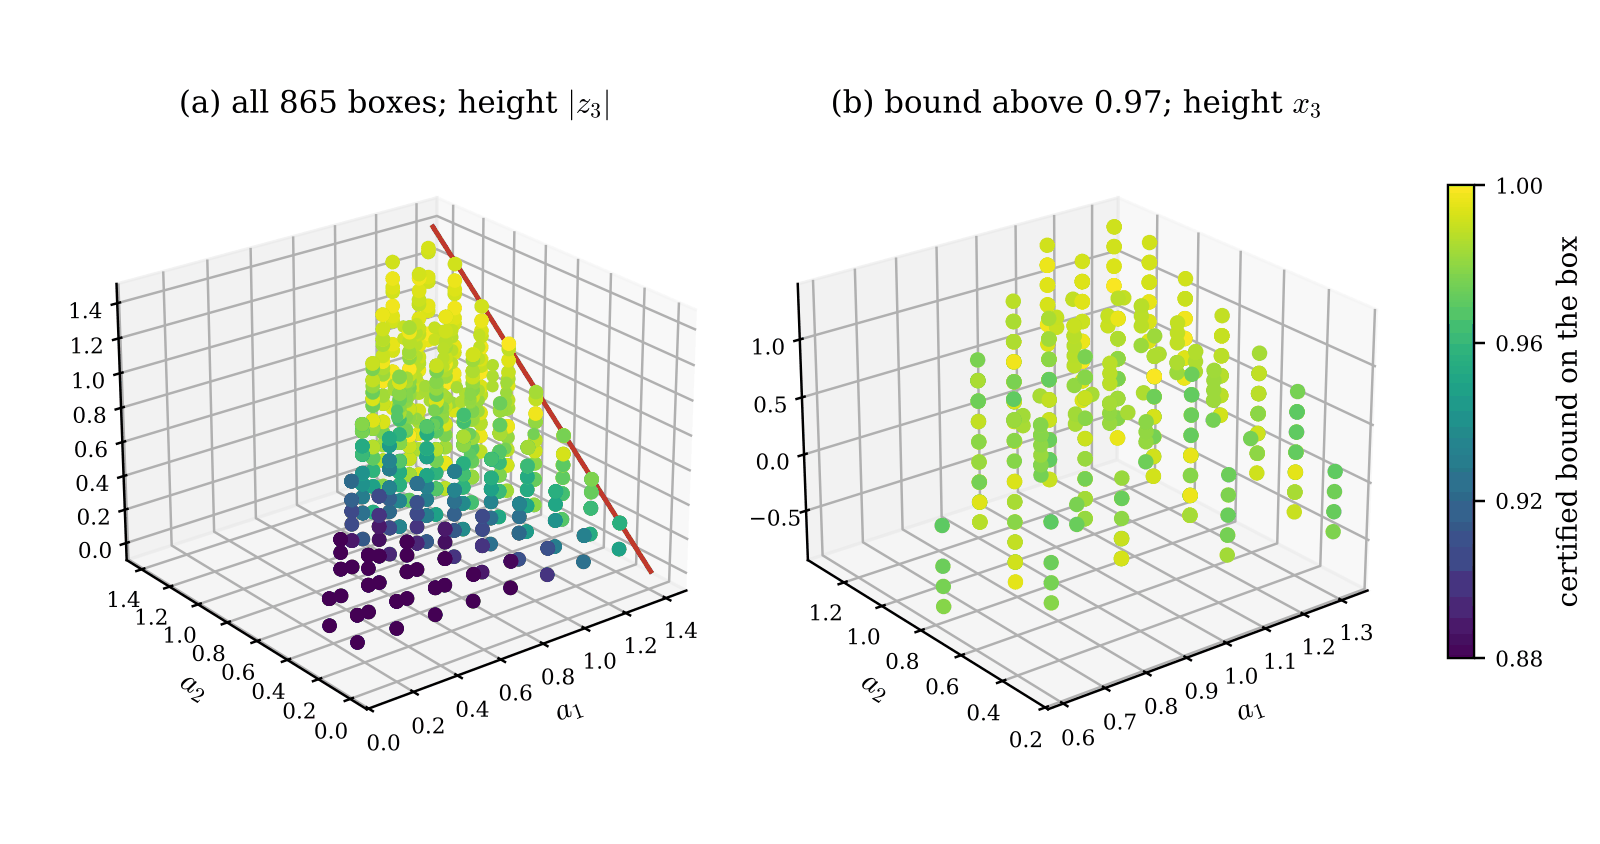
\includegraphics[width=0.92\textwidth]{figures/fig_cover.png}
\caption{The $2341$ certified boxes at $r=\frac32$, plotted at their
centres in the coordinates $(a_1,a_2)$ of the staple sum
$\operatorname{diag}(a_1,a_2,x_3+iy_3)$, coloured by the certified bound on
$2r\sup_hL_h$ over the box; the larger points are the boxes of side $r/8$.
(a) All boxes, with height $|x_3+iy_3|$. (b) The $419$ boxes with bound
above $0.99$, with height $x_3$; the largest bounds sit in the interior of
$\mathcal R_r$, not at its extreme points.}
\label{fig:cover}
\end{figure*}

\section{SU(3) with plaquette blocks}\label{sec:su3blocks}

In this section $G=\SU(3)$, $\beta\ge0$, $\beta_W=9\beta$, $N\beta=\beta_W/3$,
and the notation is that of Sec.~\ref{sec:su3}: $d$ is the Hilbert--Schmidt
distance, $K=\operatorname{conv}\SU(3)$, $\nu_c(dU)\propto e^{\ReTr(Uc)}dU$,
$\varphi_h(U)=\ReTr(Uh)$ and $\Lambda(r)$ is the modulus
of~\eqref{eq:alpha}. Put $Z(c)=\int e^{\ReTr(Uc)}dU$ and $g=\log Z$ on
$\C^{3\times3}$, viewed as $\R^{18}$ with the inner product $\ip
xy=\ReTr(xy^*)$. The gradient of $g$ at $c$ is the conjugate mean
$m(c)^*$, $m(c)=\nu_c(U)\in K$, and $\Hess g(c)(h,h)=\Var_{\nu_c}(\varphi_h)$.
Since $Z(VcW)=Z(c)$ for $V,W\in\SU(3)$, the same holds for $g$.

The blocks are those of Lemma~\ref{lem:plaqblocks}, which concerns the line
field only and holds for every group. For a block plaquette with active
links $e_1,e_2,e_3$, $\ReTr Q_p=\ReTr(y_1y_2y_3)$ with $y_i=Q_{e_i}$ or
$Q_{e_i}^{-1}$, and the conditional law of the block is
\begin{equation}\label{eq:blocklaw3}
\mu_b(dy)\propto\exp\Bigl(\sum_i\ReTr(y_ib_i)+N\beta\ReTr(y_1y_2y_3)
\Bigr)dy ,
\end{equation}
where $b_i$ is $N\beta$ times the sum of the five staples of $y_i$ outside
the block plaquette, so $b_i\in5N\beta K$ and $\|b_i\|_{\rm op}\le5N\beta$.
On $\SU(3)^3$ we use $d(y,y')=\sum_i\|y_i-y'_i\|_{\rm HS}$.

\subsection{The sensitivity of one block}

Let $r=2\beta_W=6N\beta$. Let $\lambda_*$ and $\tau$ be a lower and an upper
bound for the eigenvalues of $\Hess g$ on $rK$, $M$ an upper bound on $rK$
for $|D^3g(c)(u,v,v)|$ over unit vectors $u,v$, and $\gamma=\gamma(r)$ the
gap of Lemma~\ref{lem:gap}. Put
\begin{equation}\label{eq:blockconst3}
\begin{gathered}
w=\tfrac32(N\beta)^2(\tau-\lambda_*),\qquad s=\Lambda(r)+(e^w-1)e^w
\sqrt{\tau/\gamma},\\
C=5(N\beta)^2\Bigl(\tau s+\frac{\sqrt3\,N\beta\,M\,e^w}{\gamma}\Bigr),\\
K_3=\frac{(1+N\beta\Lambda(r))\,s}{1-C},\qquad\alpha_3=10N\beta K_3,
\end{gathered}
\end{equation}
assuming $C<1$.

\begin{lemma}\label{lem:onesite3}
Let $a,c_0\in5N\beta K$ and
\[
\kappa(dx)\propto\exp\bigl(\ReTr(xa)+g(c_0+N\beta x)\bigr)dx\quad\text{on }
\SU(3).
\]
For every $1$-Lipschitz $f$ and every $h\in\C^{3\times3}$:
\begin{enumerate}[label=\textup{(\roman*)},leftmargin=*]
\item $\Cov_\kappa(f,\varphi_h)\le s\|h\|_{\rm HS}$;
\item if $c_0$ moves in the direction $k$ inside $5N\beta K$, then
\[
\bigl|\tfrac{d}{dt}\kappa(f)\bigr|\le N\beta\bigl(\tau s+\sqrt3N\beta
Me^w/\gamma\bigr)\|k\|_{\rm HS}.
\]
\end{enumerate}
\end{lemma}

\begin{proof}
(i) The segment from $c_0$ to $c_0+N\beta x$ lies in $6N\beta K=rK$, and
Taylor's formula gives
\[
g(c_0+N\beta x)=g(c_0)+N\beta\ReTr(x\,m(c_0))+R(x)
\]
with $R(x)=\frac12(N\beta)^2\Hess g(\xi)(x,x)$. Since $\|x\|_{\rm HS}^2=3$,
$R\in[\frac32(N\beta)^2\lambda_*,\frac32(N\beta)^2\tau]$ and $\operatorname{osc}
R\le w$. Hence $\kappa$ is the tilt $e^R\nu/\nu(e^R)$ of $\nu=\nu_{c'}$ with
$c'=a+N\beta m(c_0)\in rK$. By definition of $\Lambda$, $\Cov_\nu(f,\varphi_h)
\le\Lambda(r)\|h\|$. The function $f$ is $1$-Lipschitz for the geodesic
distance, which dominates $d$, so $\mathrm{sd}_\nu f\le\gamma^{-1/2}$ by
Lemma~\ref{lem:gap}, and $\mathrm{sd}_\nu\varphi_h\le\sqrt\tau\|h\|$.
Lemma~\ref{lem:tilt} gives (i).

(ii) The derivative is $\Cov_\kappa(f,\ip{\nabla g(c_0+N\beta x)}k)$. Write
$\nabla g(c_0+N\beta u)=\nabla g(c_0)+N\beta\Hess g(c_0)u+N(u)$. The linear
term is $\varphi_h$ with $\|h\|\le N\beta\tau\|k\|$ and contributes at most
$N\beta\tau s\|k\|$ by (i). On the segment from $c_0$ the Hessian moves by at
most $N\beta M\|u\|\le\sqrt3N\beta M$, so $x\mapsto\ip{N(x)}k$ is
$\sqrt3(N\beta)^2M\|k\|$-Lipschitz for $d$. The law $\kappa$ is a tilt of
$\nu$ by a function of oscillation at most $w$, so its spectral gap is at
least $e^{-w}\gamma$ by the Holley--Stroock lemma~\cite{HS87}, and the
covariance of two Lipschitz functions under $\kappa$ is at most $e^w/\gamma$
times the product of their constants.
\end{proof}

\begin{lemma}\label{lem:blockK3}
Let $C<1$. If $b,b'$ have all fields in $5N\beta K$ and differ only in $b_i$,
then $W_1(\mu_b,\mu_{b'})\le K_3\|b_i-b'_i\|_{\rm HS}$ for the metric $d$.
\end{lemma}

\begin{proof}
By the cyclic symmetry of $\ReTr(y_1y_2y_3)$ we may take $i=1$. Given
$y_1,y_3$, the law of $y_2$ is $\nu_c$ with $c=b_2+N\beta y_3y_1\in rK$.
Changing $y_1$ by $\eta$ in $d$ moves $c$ by $N\beta\eta$ and $\nu_c$ by at most
$N\beta\Lambda(r)\eta$ in $W_1$, as in~\eqref{eq:alpha}; so $F(y_1,y_3)=
\E[f\mid y_1,y_3]$ is $(1+N\beta\Lambda(r))$-Lipschitz in each variable. The
law of $(y_1,y_3)$ is proportional to $e^{\ReTr(y_1b_1)+\ReTr(y_3b_3)}
Z(b_2+N\beta y_3y_1)$, and $Z(b_2+N\beta y_3y_1)=Z(y_3^{-1}b_2+N\beta y_1)=
Z(b_2y_1^{-1}+N\beta y_3)$, so its two conditional laws have the form of
Lemma~\ref{lem:onesite3}, with $c_0=y_3^{-1}b_2$ and $c_0=b_2y_1^{-1}$.
Moving $y_3$ to $y'_3$ moves $y_3^{-1}b_2$ along a segment in $5N\beta K$ of
length at most $\|b_2\|_{\rm op}\|y_3-y'_3\|\le5N\beta\|y_3-y'_3\|$. The
coupling argument of Lemma~\ref{lem:blockK} now gives $d_1\le s\varepsilon+
Cd_3$, $d_3\le Cd_1$ and $|\mu_b(f)-\mu_{b'}(f)|\le(1+N\beta\Lambda(r))(d_1+
d_3)\le K_3\varepsilon$.
\end{proof}

\subsection{The constants and the proof of Theorem~\ref{thm:su3blocks}}

\begin{lemma}\label{lem:su3const}
At $r=\frac32$ every eigenvalue of $\Hess g$ on $rK$ lies in
$[0.056015,0.247316]$, and $|D^3g(c)(u,v,v)|\le0.182126$ for $c\in rK$ and
unit vectors $u,v$. At $r=\frac{38}{25}$ the same holds with
$[0.054978,0.248280]$ and $0.183546$.
\end{lemma}

\begin{proof}
For $V,W\in\SU(3)$, $g(VcW)=g(c)$ and $x\mapsto VxW$ is an isometry, so the
eigenvalues of $\Hess g$ and the norm of $D^3g$ are constant on the orbits,
and by Lemma~\ref{lem:orbits} it suffices to bound them on $\mathcal R_r$. The
derivatives of $g$ are the cumulants of $\varphi$ under $\nu_c$. Cut the box
$[0,r]^2\times[-r,r]\times[0,r]$ into boxes of side $r/8$ and keep the $841$
($784$ at $r=\frac{38}{25}$) that survive the two tests of Sec.~\ref{ssec:cover}. On each box $Q$ we
compute, with rigorous error bounds, the moments of $\varphi$ of degree at
most three at the sixteen corners $b_i$ and at the centre $b_0$, and put
$k=m(b_0)$, the mean of $\varphi$ at the centre.

\emph{Upper bound.} For $b\in Q$ and every $h$, $\Var_{\nu_b}(\varphi_h)\le
\nu_b[(\varphi_h-\ip kh)^2]\le e^{\varsigma/8}\max_i\nu_{b_i}[(\varphi_h-
\ip kh)^2]$ by Lemma~\ref{lem:boxes}(ii).

\emph{Lower bound.} Integrating the right inequality of~\eqref{eq:hoeffding}
against $f\ge0$ and dividing by $Z(b)\le\sum_i\omega_iZ(b_i)$, the left one,
gives $\nu_b(f)\ge
e^{-\varsigma/8}\min_i\nu_{b_i}(f)$. With $f=(\varphi_h-\nu_b\varphi_h)^2$ this
gives $\Var_{\nu_b}(\varphi_h)\ge e^{-\varsigma/8}\min_i\Var_{\nu_{b_i}}
(\varphi_h)$.

\emph{Third cumulant.} Put $\delta=m(b)-k$. The mean value theorem and the
upper bound give $\|\delta\|\le\tau\rho+e$, with $\rho$ the largest distance
from $b_0$ in $Q$ and $e$ the error of the computed mean. Expanding the
central moment about $k$,
\[
\begin{aligned}
D^3g(b)(u,v,v)&=T_b(u,v,v)-\delta_u\Var(\varphi_v)\\
&\quad-2\delta_v\Cov(\varphi_u,\varphi_v)-\delta_u\delta_v^2 ,
\end{aligned}
\]
with $T_b=\nu_b[(\varphi-k)^{\otimes3}]$, $\delta_u=\ip\delta u$ and the
moments under $\nu_b$. For a function $G$ of either sign, writing $G=G^+-G^-$
and applying the two bounds above to $G^\pm$ gives
$|\nu_b(G)|\le(\max_i|\nu_{b_i}(G)|+\varepsilon\max_i\nu_{b_i}|G|)/(1-
\varepsilon)$ with $\varepsilon=1-e^{-\varsigma/8}$. For $G=(\varphi_u-k_u)
(\varphi_v-k_v)^2$ we use $|\nu_{b_i}(G)|\le\|T_{b_i}\|$, the largest singular
value of the $18\times324$ unfolding of $T_{b_i}$, and $\nu_{b_i}|G|\le2\sqrt3
\,\nu_{b_i}[(\varphi_v-k_v)^2]$, since $\|U-k\|_{\rm HS}\le2\sqrt3$. The
largest eigenvalues and singular values are bounded as in
Sec.~\ref{ssec:cover}, and the maxima over these boxes are the numbers
stated (Appendix~\ref{app:plaqblocks}).
\end{proof}

\begin{proof}[Proof of Theorem~\ref{thm:su3blocks}]
Let first $\beta_W\le\frac34$, so that $r=2\beta_W\le\frac32$. Every field
met in Lemmas~\ref{lem:onesite3} and~\ref{lem:blockK3} lies in $\frac32K$, so
the constants of Lemma~\ref{lem:su3const} at $\frac32$,
$\Lambda(\frac32)\le\frac{0.999887}3$ from Proposition~\ref{prop:cover} and
$\gamma=\gamma(\frac32)=\frac{187}{128}$ apply; with these fixed constants every
quantity in~\eqref{eq:blockconst3} is increasing in $\beta_W$. For
$\frac34<\beta_W\le\frac{19}{25}$ the fields lie in $\frac{38}{25}K$, and the
constants of Lemma~\ref{lem:su3const} at $\frac{38}{25}$,
$\Lambda(\frac{38}{25})\le\frac{1.029967}{3.04}$ from
Proposition~\ref{prop:cover2} and $\gamma(\frac{38}{25})=\frac{4643}{3200}$
apply in the same way. Changing an active link $j$ by $\eta$ changes one
staple of each of its ten partners outside its block by a matrix of norm
$\eta$, so the field $b_i$ of each such partner moves by $N\beta\eta$, and
Lemma~\ref{lem:blockK3} gives $\sum_BC_{Bj}\le10N\beta K_3=\alpha_3(\beta_W)$.
In ball arithmetic, at $\beta_W=\frac34$, $w\le0.017935$, $s\le0.34088$,
$C\le0.043520$, $K_3\le0.38609$ and $\alpha_3\le0.96521$; at $\beta_W=0.72$,
$\alpha_3\le0.91815$; at $\beta_W=0.76$, with the second set of constants,
$w\le0.018609$, $s\le0.34673$, $C\le0.045770$, $K_3\le0.39454$ and
$\alpha_3\le0.99950$. Proposition~\ref{prop:blockstate}, whose proof does not
use the group, applies with the Hilbert--Schmidt metric.
\end{proof}

\begin{remark}\label{rem:su3blocks}
Theorem~\ref{thm:su3} ends where $2r\Lambda(r)$ reaches one. The blocks
remove the factor $\frac{12}{10}$ of the single-link sum and keep most of it
after paying for the three links: at $\beta_W=\frac34$ the gap bound rises
from $1.1\cdot10^{-4}$ to $0.0177$, and the block bound is the better one for
$\beta_W\ge0.715$. Before the corrections for the three links their sum is
$\frac{10}{12}$ of the single-link sum $2r\Lambda(r)$, so it can stay below one
while $2r\Lambda(r)$ is slightly above one; Proposition~\ref{prop:cover2} certifies
$2r\Lambda(r)\le1.03$ at $r=1.52$, which is enough at $\beta_W=0.76$, with
little room. Evaluated in floating point with the constants of a scan of
$\mathcal R_r$, the block sum stays below one up to $\beta_W\approx0.78$;
that computation is not certified and is not used.
\end{remark}

\section{Where the methods stop}\label{sec:limits}

\emph{$\SU(2)$.} Theorem~\ref{thm:ceiling} closes the single-link route in
every forest gauge at $\beta_W=\frac13$. Blocks of several links, where the
influence of a boundary link on a whole block is bounded at once, in the
spirit of the Dobrushin--Shlosman criterion~\cite{DS85}, pass it:
plaquette blocks reach $\beta_W=0.345$ (Theorem~\ref{thm:blocks}), and the
sharper floating-point bound of Remark~\ref{rem:blockgap} stops near
$0.357$. Larger blocks are the next step.

\emph{Curvature.} Remark~\ref{rem:hf} locates the end of the curvature
method in this gauge between $|\beta|=1/28.840002$, by the
certificate of Appendix~\ref{app:certificate}, and $\frac1{26.25}$.

\emph{$\SU(3)$.} The route of Sec.~\ref{sec:su3} bounds the
$H^{-1}(\nu_b)$ norm of $\varphi_h-\nu_b\varphi_h$, which is at least
$L_h(b)$, and needs it uniformly on $rK$. Its Galerkin values (polynomials
of degree two) at matrices of $rK$ give $2r$ times the norm equal to $0.79$
at $r=1.25$, $0.89$ at $r=1.4$, $0.97$ at $r=1.5$ and $1.009$ at $r=1.55$, so
the route stops at or below $\beta_W\approx0.77$ even with exact constants.
With $u=s\varphi_h$, Lemma~\ref{lem:corrector} stops earlier: in floating
point its largest values on $\mathcal R_r$ lie on the face
$\operatorname{diag}(r,\rho,\rho)$ with $\rho$ between $0.75r$ and $0.8r$, and
$2r$ times the bound is $0.9458$ at $r=1.36$, $0.9767$ at $r=1.40$ and $1.0080$
at $r=1.44$, so this corrector ends near $\beta_W\approx0.715$. With $u=q_h$
of degree two the largest values on the same face are $0.9305$ at $r=1.44$,
$0.9729$ at $r=1.50$ and $1.0018$ at $r=1.54$ (Fig.~\ref{fig:face}), close to the
Galerkin values. Lemma~\ref{lem:gap} therefore costs
little at these couplings, and most of the distance between the
floating-point value at $r=1.5$ and the certified $0.999887$ of
Proposition~\ref{prop:cover} is the interpolation over boxes. Between
$\beta_W=\frac34$ and $0.77$ there is room only for smaller boxes. The
plaquette blocks of Theorem~\ref{thm:su3blocks} use $\Lambda(2\beta_W)$ as
well, with a little more room: they reach $0.76$ with the certified cover of
Proposition~\ref{prop:cover2} and near $0.78$ in floating point
(Remark~\ref{rem:su3blocks}); past that one needs larger blocks, whose
sensitivity does not go through the one-link modulus.

\begin{figure*}[t]
\centering
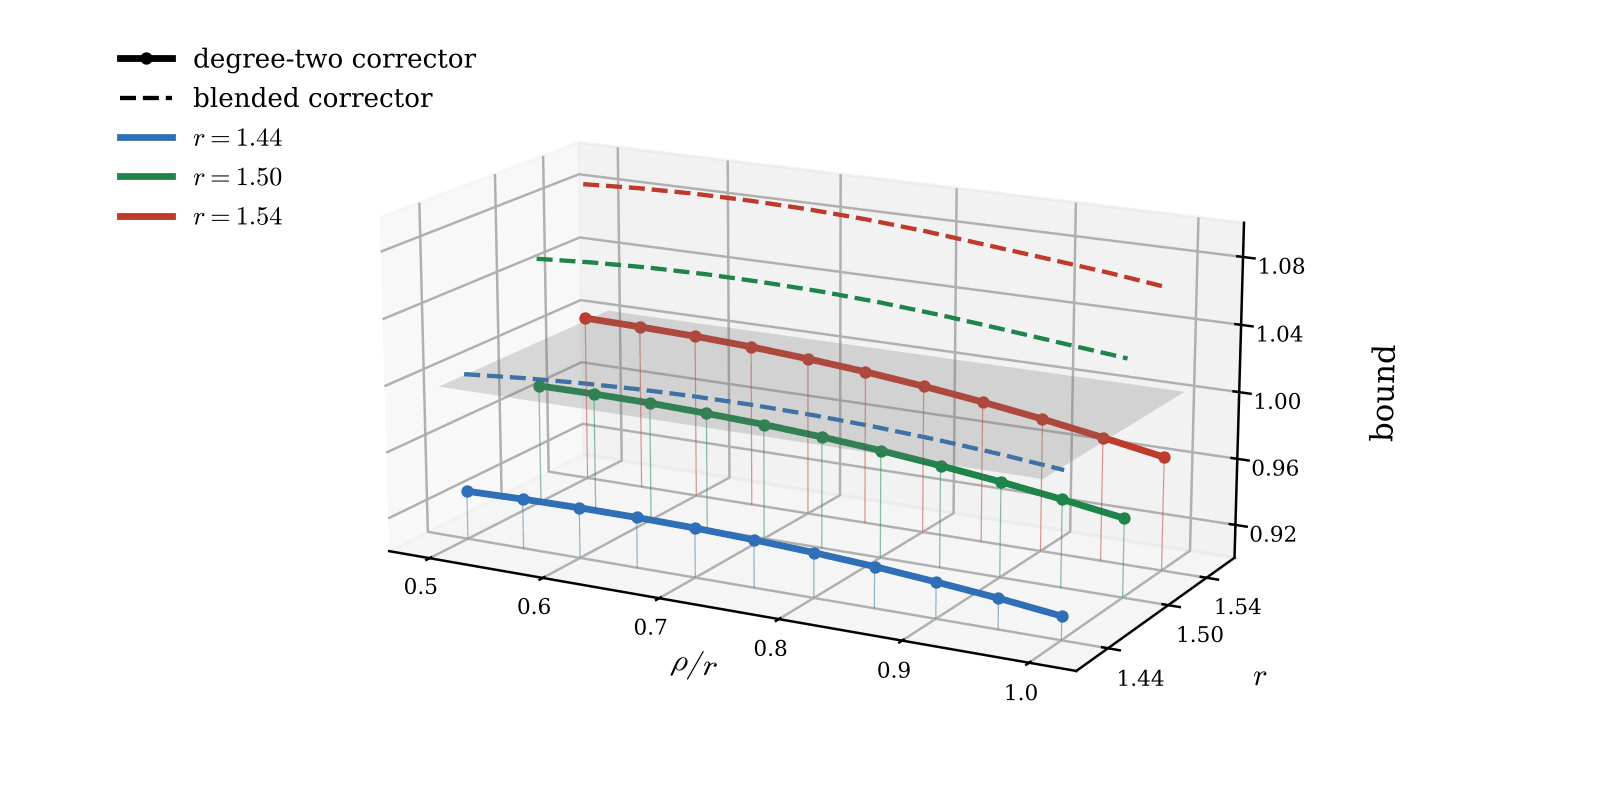
\includegraphics[width=0.84\textwidth]{figures/fig_face.png}
\caption{The floating-point value of $2r\sup_h$ of the bound of
Lemma~\ref{lem:corrector} on the face $b=\operatorname{diag}(r,\rho,\rho)$, as
a function of $\rho/r$, for $r=1.44$, $1.50$ and $1.54$: dashed with the
corrector $u=s\varphi_h$ for the best $s$, solid with $u=q_h$ of degree two
for the best $C$. The grey plane is the Dobrushin threshold one. The first
corrector is above it already at $r=1.44$; the second stays below it at
$r=1.50$, where Proposition~\ref{prop:cover} certifies the bound on all of
$\mathcal R_r$, and crosses it by $r=1.54$.}
\label{fig:face}
\end{figure*}

\emph{Other groups.} For groups other than $\SU(2)$ and $\SU(3)$ only the
curvature route is carried out here (Theorem~\ref{thm:groups}), and it stops
where the bound $\frac{29}2$ uses up the curvature of $G$, at
$N|\beta|=\frac2{29}\kappa_G$. The Dobrushin route needs a bound for the Kantorovich
modulus of the one-link measure of each group, which is not attempted here.

\emph{The four open problems.} Our earlier paper~\cite{BB26a} listed four
problems between the strong-coupling results and the Clay
problem~\cite{JW06}: (1) uniqueness and a gap at intermediate fixed
coupling; (2) the crossover from strong coupling to Ba{\l}aban's
weak-coupling regime; (3) the continuum limit with the
Osterwalder--Schrader axioms; and (4) a gap in physical units. The present
paper moves the boundary of (1): for $\SU(2)$ from $\beta_W=\frac29$ to
$0.345$, for $\SU(3)$ from $\frac9{32}$ to $0.76$, with a gap at $\frac34$ of
$0.0177$ in lattice units, and for every compact simple
group, the exceptional groups included, past the curvature ceiling of the
ungauged measure, with an explicit gap. It does not close (1); the region
between these values and the scaling region, near $\beta_W\approx2.2$ for
$\SU(2)$ and $\beta_W\approx6$ for $\SU(3)$, is open, and with it problem
(2). Problems (3) and (4) are not solved here. Every bound proved here is uniform
in lattice units, so by~\cite{BB26b} none of them can by itself produce a
continuum mass gap; that requires control of the gap in physical units along
the renormalisation group flow~\cite{Bal84a,BSB26}.\footnote{Every one of these approaches needs an input at physical
length scales. Renormalisation group approaches to the ultraviolet behaviour
of gauge and gravitational theories, of which~\cite{Bal84a,Dim13} are the
rigorous ones for Yang--Mills theory, have also been proposed for the
effective dimension of spacetime~\cite{SBG26} and for completions of quantum
gravity~\cite{Bha22,BRS26}; they do not bear on the infrared estimates
needed here.}

\emph{The continuum problem.} Two general facts limit what can be imported
into problems (3) and (4) above from constructions of continuum measures.
Both concern a random distribution $F$ on $\R^d$, a Borel probability
measure on the tempered distributions with finite moments, and the growth
condition
\begin{equation}\label{eq:growth}
\E\,e^{F(\chi)}\le e^{C(\|\chi\|_1+\|\chi\|_2^2)}\qquad\text{for all real }
\chi\in\mathcal S(\R^d),
\end{equation}
which is the growth condition of the regularity axiom of Glimm and Jaffe at
$p=2$~\cite[Sect.~6.1, (6.1.5)]{GJ87}. The next proposition shows that it
rules out every field whose two-point function is too singular at short
distance.

\begin{proposition}\label{prop:growth}
Let $F$ satisfy~\eqref{eq:growth}, and suppose that its connected two-point
function is, off the diagonal, a locally integrable function $S_2(x,y)$
with $S_2(x,y)\ge c|x-y|^{-2\Delta}\bigl(\log\frac1{|x-y|}\bigr)^{-k}$ for
$0<|x-y|\le r_0$, where $c>0$, $k\ge0$ and $2\Delta>d$. Then $F$ does not
exist: no random distribution has both properties.
\end{proposition}

\begin{proof}
Applying~\eqref{eq:growth} to $\chi$ and $-\chi$ and using $\cosh x\ge1+\frac{x^2}2$
gives $\E F(\chi)^2\le2(e^{C(\|\chi\|_1+\|\chi\|_2^2)}-1)$. Fix nonnegative
$\varphi,\psi\in C_c^\infty(\R^d)$, not zero, with supports in a ball of
radius $\frac R2$ and at distance $\delta>0$ from each other, and put
$\varphi_\varepsilon(x)=\varepsilon^{-d/2}\varphi(x/\varepsilon)$, and likewise
$\psi_\varepsilon$. Then $\|\varphi_\varepsilon\|_2=\|\varphi\|_2$ and
$\|\varphi_\varepsilon\|_1=\varepsilon^{d/2}\|\varphi\|_1\le\|\varphi\|_1$ for
$\varepsilon\le1$, so the covariance of $F(\varphi_\varepsilon)$ and
$F(\psi_\varepsilon)$ is bounded uniformly in $\varepsilon$ by the
Cauchy--Schwarz inequality. On the other hand the supports of
$\varphi_\varepsilon$ and $\psi_\varepsilon$ are disjoint, and for $u,v$ in the
supports $\varepsilon\delta\le|\varepsilon u-\varepsilon v|\le\varepsilon R$.
For $\varepsilon R\le r_0$ and $\varepsilon R<1$ the lower bound for $S_2$
therefore gives
\[
\begin{split}
\Cov\bigl(F(\varphi_\varepsilon),F(\psi_\varepsilon)\bigr)&=\varepsilon^d\!\int\!\!\int
\varphi(u)\psi(v)S_2(\varepsilon u,\varepsilon v)\,du\,dv\\
&\ge c\,R^{-2\Delta}\varepsilon^{d-2\Delta}\Bigl(\log\frac1{\varepsilon\delta}\Bigr)^{-k}
\|\varphi\|_1\|\psi\|_1 ,
\end{split}
\]
which tends to infinity as $\varepsilon\to0$.
\end{proof}

The action density $\Tr F_{\mu\nu}F_{\mu\nu}$ has dimension $\Delta=4$ in four
dimensions. A two-sided short-distance law of the form $|x-y|^{-8}$ times
the fourth power of the running coupling, which is what asymptotic freedom\footnote{For $\SU(N)$ the renormalisation group gives, with $b_0=11N/(48\pi^2)$ and the invariant scale $\Lambda$,
\[
g(a)^{-2}=2b_0\log\tfrac1{a\Lambda}+O\bigl(\log\log\tfrac1{a\Lambda}\bigr),
\]
so the inverse coupling $\beta_W=2N/g(a)^2$ grows like $\frac{11N^2}{12\pi^2}\log\frac1{a\Lambda}$ along the continuum tuning.}
predicts, has $2\Delta=8>4$ and $k=2$; so that field
cannot satisfy~\eqref{eq:growth}, and a proof of rotation invariance for it
has to use something other than this condition. In three dimensions the free part of the action density
already has $2\Delta=6>3$. Condition~\eqref{eq:growth} suits fields of
dimension at most $\frac d2$, such as the field strength of the free Maxwell
field, whose covariance is bounded in momentum space.

Positivity, symmetry and regularity do not produce a gap by themselves.

\begin{proposition}\label{prop:nogapgff}
On $\R^4$ let $F$ be the centred Gaussian random distribution with
covariance
\[
\widehat C(p)=\int_0^1\frac{m^2}{|p|^2+m^2}\,dm .
\]
Then $F$ is invariant under all Euclidean motions, reflection positive,
satisfies~\eqref{eq:growth} with $C=\frac12$, and its Osterwalder--Schrader
Hamiltonian has no gap above the vacuum.
\end{proposition}

\begin{proof}
Since $0\le\widehat C\le1$, $\E e^{F(\chi)}=e^{\frac12\ip\chi{C\chi}}\le e^{\frac12
\|\chi\|_2^2}$, with the unitary Fourier transform. Invariance is clear. The
covariance is the integral over $m\in(0,1)$, with the weight $m^2dm$, of the
covariances of free fields of mass $m$, each of which is reflection
positive~\cite[Sect.~6.2]{GJ87}; a positive combination of reflection
positive covariances is reflection positive, and so is the Gaussian measure
with such a covariance~\cite[Sect.~6.2]{GJ87}. For $\chi(t,\mathbf x)=h(t)g(\mathbf x)$
with $h\ge0$ supported in $t>0$, not zero, and $\hat g(0)\ne0$, the vector
$v=F(\chi)$ is orthogonal to the vacuum, and after the Fourier transform in
$\mathbf x$,
\[
\begin{split}
\ip v{e^{-sH}v}={}&\int_0^1m^2\,dm\int\frac{|\hat g(\mathbf k)|^2}{2\omega}
e^{-\omega s}\\
&\times\Bigl(\int_0^\infty h(t)e^{-\omega t}dt\Bigr)^2\,d\mathbf k ,
\end{split}
\]
with $\omega=\sqrt{|\mathbf k|^2+m^2}$ and constants absorbed in $\hat g$.
If $H$ had a gap $m_0>0$, the left side would be at most $e^{-m_0s}\|v\|^2$.
For $0<\eta<m_0$ the part of the integral with $m,|\mathbf k|\le\eta/2$ is at
least $c_\eta e^{-\eta s}$ with $c_\eta>0$, a contradiction as $s\to\infty$.
\end{proof}

The Gaussian field of Proposition~\ref{prop:nogapgff} is not a gauge theory;
it shows only that an infrared estimate, such as a bound
$\ip{v_a}{T_a^{\lfloor t/a\rfloor}v_a}\le C_ve^{-m_*t}$ uniform in the spacing $a$
along the continuum tuning, has to be proved in addition to the axioms. The
lattice bounds of this paper are of this form only with $m_*$ proportional
to $1/a$, and by~\cite{BB26b} such bounds give trivial limits. The routes we
know to a continuum gap therefore all stop at the same two estimates: the
construction of the infinite-volume continuum measure past
Ba{\l}aban's small-field analysis~\cite{Bal84a,Bal89b}, and a decay estimate in physical
units at large scales.

\section{The continuum step at one physical scale}\label{sec:bypass}

The bounds of the preceding sections hold at fixed coupling and give a gap
that is at least a fixed number in lattice units, and~\cite{BB26b} shows that
no such bound can produce a continuum gap. This section replaces the
single-link condition of Proposition~\ref{prop:state} by a condition on one
cube of $n^4$ sites, averaged over its translates in the manner of Dobrushin
and Shlosman~\cite{DS85}, and proves that the condition gives a gap of order
$1/n$ in lattice units. If it holds with $n$ proportional to $1/a$, that is,
in a cube of fixed physical size, the gap survives in physical units and
passes to every continuum limit (Theorem~\ref{thm:transfer}). The two
statements that remain unproved, the cube estimate and the existence of the
limit, are stated in Sec.~\ref{sec:inputs}.

\subsection{Averaged cubes}

For a finite set $V\subset A$ let $\gamma_V(\cdot\mid Q)$ be the probability
measure on $G^V$ with density proportional to $\exp\bigl(N\beta\sum_{p\cap
V\ne\emptyset}\ReTr Q^F_p\bigr)$ with respect to Haar measure, the links
outside $V$ being those of $Q$. Its conditional law of $Q_e$, $e\in V$, given
the other links of $V$ is $\gamma^F_e$. Write $d_V(Q_V,Q'_V)=\sum_{i\in V}
\delta(Q_i,Q'_i)$ and, for $j\in A\setminus V$,
\[
C_{V,j}=\sup\frac{W_1^{d_V}\bigl(\gamma_V(\cdot\mid Q),\gamma_V(\cdot\mid
Q')\bigr)}{\delta(Q_j,Q'_j)},
\]
the supremum over pairs that differ only at $j$; $W_1^{d_V}$ is the
Kantorovich distance for $d_V$. The coefficient vanishes unless $j$ shares a
plaquette with a link of $V$.

Let $n\ge2$ be even and let $V$ be the set of active links $(x,\mu)$ with
$x\in[0,n)^4$. The direction field has period two, so the translations by
$2\Z^4$ preserve $F$, $A$ and $\gamma^F$, and the translates $V_x=V+x$,
$x\in2\Z^4$, satisfy $C_{V_x,j+x}=C_{V,j}$. Every active link lies in exactly
$N_n=(n/2)^4$ of them. A \emph{class} is an orbit of $2\Z^4$ on $A$, that is,
a residue of the base point modulo two together with a direction; there are
at most $64$ classes. For a class $c$ put
\[
K_c=\sum_{j\in c\setminus V}C_{V,j}.
\]

\begin{definition}\label{def:cube}
For $0<\alpha<1$, the condition $D(n,\alpha)$ at the coupling $\beta$ is
$K_c\le\alpha N_n$ for every class $c$.
\end{definition}

Since $\sum_{x\in2\Z^4,\,j\notin V_x}C_{V_x,j}=\sum_{x}C_{V,j-x}[j-x\notin V]
=K_{c(j)}$ for the class $c(j)$ of $j$, the condition says that the total
influence of a link on the translates that do not contain it is at most the
fraction $\alpha$ of the number of translates that do. Figure~\ref{fig:cubes} shows the cubes.

\begin{figure*}[t]
\centering
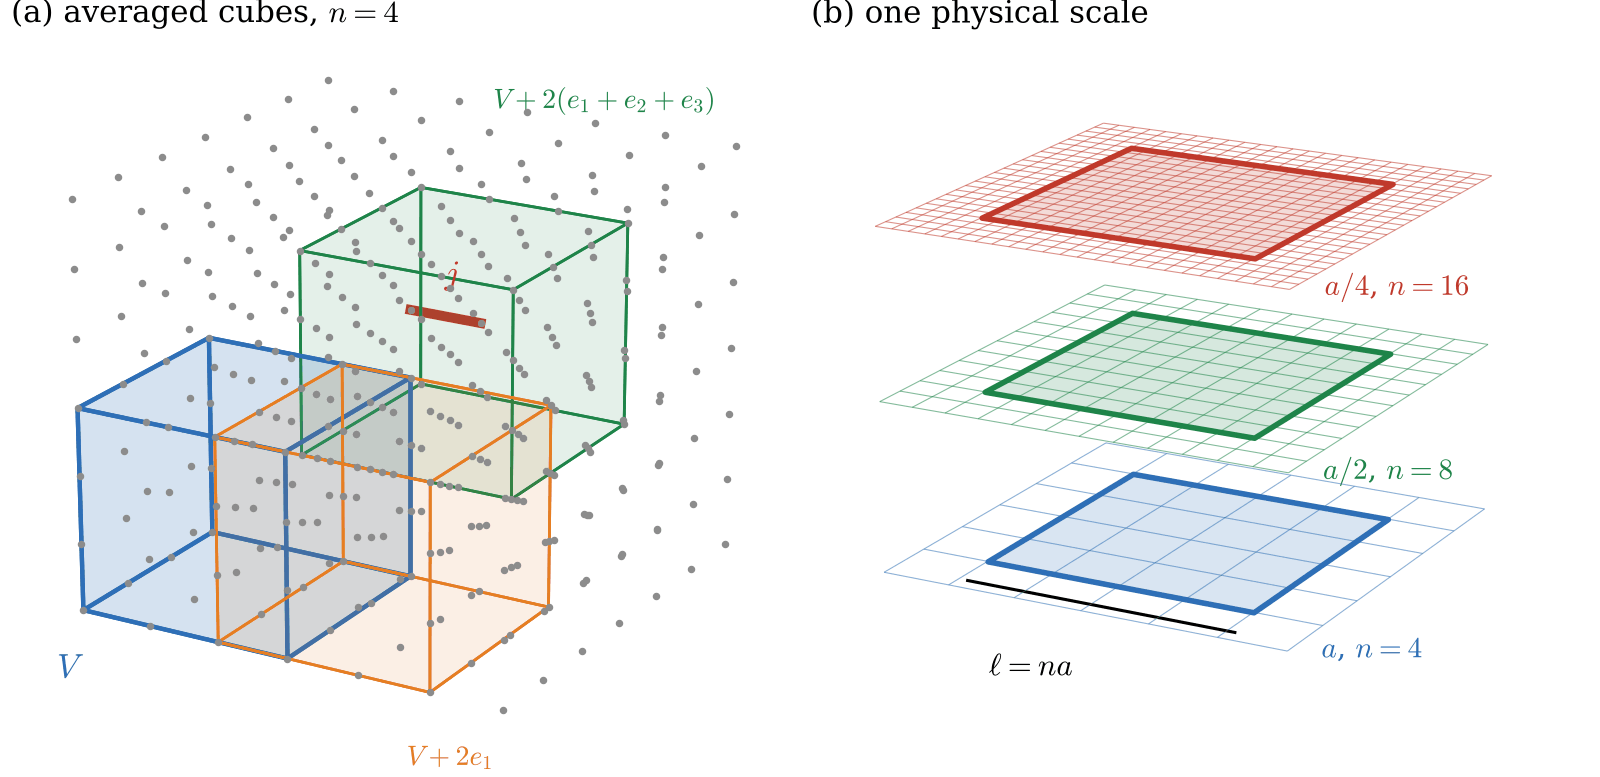
\includegraphics[width=0.9\textwidth]{figures/fig_cubes.png}
\caption{(a) The cube $V$ of side $n=4$ and two of its translates by
$2\Z^4$, drawn in three of the four dimensions. A link $j$ outside $V$
enters $K_c$ through every translate whose boundary it touches, and
$D(n,\alpha)$ compares that total with the $N_n=(n/2)^4$ translates that
contain $j$. (b) The cube of Theorem~\ref{thm:transfer}: its physical side
$\ell=na$ is held fixed while the spacing is halved, so $n$ doubles at each
step and the lattice gap $\log(1/\alpha)/(2n)$ is of order $a/\ell$.}
\label{fig:cubes}
\end{figure*}
 For $n=2$ it is a
bound on blocks of $48$ links. Distances between links are those of their
midpoints; a link of $V$ and a link sharing a plaquette with $V$ are at
distance at most $\rho_n=2n$, and $c_n$ denotes the number of active links
within distance $\rho_n$ of a given one.

\begin{theorem}\label{thm:onescale}
Let $\beta\ge0$ and suppose that $D(n,\alpha)$ holds. Then statements
\textup{(i)}--\textup{(iv)} of Proposition~\ref{prop:state} hold,
\textup{(v)} holds for every $\lambda<\log(1/\alpha)/\rho_n$, and the transfer
matrix of $\omega$ has spectral gap at least $\log(1/\alpha)/(2n)$.
\end{theorem}

\begin{proof}
The proof of Proposition~\ref{prop:state} uses the coefficients $C_{ee'}$
only through Lemma~\ref{lem:comparison} and Corollary~\ref{cor:decay}.
Lemma~\ref{lem:dscomparison} of Appendix~\ref{app:comparison} gives the same
conclusions under $D(n,\alpha)$, for every $\lambda>0$ with $\alpha
e^{\lambda\rho_n}<1$, with the constant $\theta D/(1-\theta)$ replaced by
$D(1+c_ne^{\lambda\rho_n})/(1-\theta)$ and $\theta=\alpha e^{\lambda\rho_n}$.
The measures used there are invariant under every $\gamma_{V_x}$ with $V_x$
disjoint from the exceptional set: a Gibbs measure of $\gamma^F$ and its
conditional measures given the links of a finite set by
Lemma~\ref{lem:dscomparison}(a), and the extended finite-volume measure of
part (ii) because every plaquette that meets such a $V_x$ lies in
$P(\Lambda)$. Part (vi) then follows from Proposition~\ref{prop:gapdecay}
as before, with every $\lambda<\log(1/\alpha)/(2n)$.
\end{proof}

\subsection{The continuum limit}

Let $a_k=2^{-k}a_0$ and let $\beta_k\ge0$ be couplings, typically with
$\beta_k\to\infty$. Suppose that the lattice states $\omega_k$ at $\beta_k$
exist as in Proposition~\ref{prop:state}, with transfer matrices $\mathbb T_k$ on
the reconstructed spaces $\mathcal H_k$ and vacua $\Omega_k$
(Appendix~\ref{app:transfer}). Let $\mathcal T$
be a complex vector space of test functions on $\R^4$ supported in $\{t>0\}$
and, for each $k$, let $f\mapsto O_k(f)$ be a linear map from $\mathcal T$ to
gauge-invariant local observables supported in positive lattice times; the
example to keep in mind is $O_k(f)=Z_k\sum_xa_k^4f(a_kx)\Phi(x)$ for a local
gauge-invariant field $\Phi$, a renormalisation constant $Z_k$ and $\Phi(x)$
the translate of $\Phi$ to $x$. Write $\vartheta$ for the time reflection and
$\tau_t$ for the time translation by $t$ lattice steps.

\begin{definition}\label{def:limit}
A \emph{continuum limit} of $(\omega_k,O_k)$ is a Hilbert space $\mathcal H$
with a unit vector $\Omega$, a self-adjoint operator $H\ge0$ with
$H\Omega=0$, and a linear map $f\mapsto\psi(f)$ from $\mathcal T$ to
$\mathcal H$ with dense range, such that for all $f,g\in\mathcal T$ and all
dyadic $\tau\ge0$,
\[
\begin{split}
\ip{\psi(f)}{e^{-\tau H}\psi(g)}&=\lim_{k\to\infty}\omega_k\bigl(\vartheta
(\overline{O_k(f)})\,\tau_{\tau/a_k}O_k(g)\bigr),\\
\ip\Omega{\psi(f)}&=\lim_{k\to\infty}\omega_k\bigl(O_k(f)\bigr),
\end{split}
\]
the limits taken over the $k$ for which $\tau/a_k$ is an integer. It is
\emph{nontrivial} if $\mathcal H\ne\C\Omega$.
\end{definition}

The Osterwalder--Schrader reconstruction~\cite{OS73,OS75} produces such a
limit from convergent renormalised Schwinger functions that satisfy the
axioms; the definition records only what the next theorem uses.

\begin{theorem}\label{thm:transfer}
Suppose that there are $\alpha<1$, $\ell>0$ and even $n_k$ with
$n_ka_k\le\ell$ such that $D(n_k,\alpha)$ holds at $\beta_k$ for every $k$.
Then every continuum limit of $(\omega_k,O_k)$ satisfies
\[
\sigma(H)\subset\{0\}\cup[m_*,\infty),\qquad m_*=\frac{\log(1/\alpha)}{2\ell},
\]
and $0$ is a simple eigenvalue. If the limit is nontrivial,
$\sigma(H)\cap[m_*,\infty)\ne\emptyset$, so $H$ has a mass gap of at least
$m_*$.
\end{theorem}

\begin{proof}
By Theorem~\ref{thm:onescale} the state $\omega_k$ exists and $\mathbb T_k$ has gap
at least $\log(1/\alpha)/(2n_k)$ on the complement of $\Omega_k$. Let $f\in
\mathcal T$, put $O=O_k(f)$ and $\varphi_k=\Psi_O-\omega_k(O)\Omega_k$. In
the reconstruction of Appendix~\ref{app:transfer},
$\ip{\Psi_F}{\mathbb T_k^t\Psi_H}=\omega_k(\vartheta(\bar F)\tau_tH)$, so
$\ip{\Omega_k}{\Psi_O}=\omega_k(O)$, and $\mathbb T_k\Omega_k=\Omega_k$; hence, for integers $t\ge0$,
\[
\begin{split}
\ip{\varphi_k}{\mathbb T_k^t\varphi_k}&=\omega_k\bigl(\vartheta(\bar O)\,\tau_tO\bigr)
-|\omega_k(O)|^2\\
&\le e^{-t\log(1/\alpha)/(2n_k)}\,\|\varphi_k\|^2 .
\end{split}
\]
Take $\tau\ge0$ dyadic and $k$ large, so that $t=\tau/a_k$ is an integer;
then $t/(2n_k)=\tau/(2n_ka_k)\ge\tau/(2\ell)$, and the right side is at most
$e^{-m_*\tau}\|\varphi_k\|^2$. Both sides converge by
Definition~\ref{def:limit}. With $\varphi=\psi(f)-\ip\Omega{\psi(f)}\Omega$
and $e^{-\tau H}\Omega=\Omega$ the limit reads
\[
\ip\varphi{e^{-\tau H}\varphi}\le e^{-m_*\tau}\|\varphi\|^2 .
\]
The maps $f\mapsto O_k(f)$ and $f\mapsto\psi(f)$ are linear, so the vectors
$\varphi$ form a linear subspace, and it is dense in $\Omega^\perp$ because
the range of $\psi$ is dense. The inequality extends to $\Omega^\perp$ by
continuity, and from dyadic $\tau$ to all $\tau\ge0$ by the strong continuity
of $e^{-\tau H}$. For $\varphi\in\Omega^\perp$ with spectral measure
$\mu_\varphi$ of $H$ this says $\int e^{-\tau E}d\mu_\varphi(E)\le e^{-m_*\tau}
\mu_\varphi([0,\infty))$ for all $\tau\ge0$; if $\mu_\varphi([0,m_*-\eta])>0$
for some $\eta>0$, the left side is at least $\mu_\varphi([0,m_*-\eta])
e^{-(m_*-\eta)\tau}$, which exceeds the right side for large $\tau$. So
$\mu_\varphi$ lives on $[m_*,\infty)$ for every $\varphi\in\Omega^\perp$, which
gives both claims about $0$, and the spectrum on $\Omega^\perp\ne\{0\}$ lies in
$[m_*,\infty)$ and is not empty.
\end{proof}

The proof uses $D(n_k,\alpha)$ only through the decay of the two-point
functions, and the same argument accepts any decay with constants that
depend on the observable.

\begin{theorem}\label{thm:clustering}
Let $m_0>0$ and let $\mathcal T_0$ span $\mathcal T$. Suppose that for each
$f\in\mathcal T_0$ there are $C_f<\infty$, $\tau_f\ge0$ and $k_f$ such that
\begin{align*}
C^f_k(\tau)&=\omega_k\bigl(\vartheta(\overline{O_k(f)})\,\tau_{\tau/a_k}
O_k(f)\bigr)-|\omega_k(O_k(f))|^2\\
&\le C_fe^{-m_0\tau}
\end{align*}
for all $k\ge k_f$ and all dyadic $\tau\ge\tau_f$ with $\tau/a_k\in\Z$.
Then every continuum limit of $(\omega_k,O_k)$ satisfies $\sigma(H)\subset
\{0\}\cup[m_0,\infty)$, and $0$ is a simple eigenvalue. If the limit is
nontrivial, $H$ has a mass gap of at least $m_0$.
\end{theorem}

\begin{proof}
For $f\in\mathcal T$ put $\varphi(f)=\psi(f)-\ip\Omega{\psi(f)}\Omega$,
which is linear in $f$. Since $e^{-\tau H}$ is self-adjoint and fixes
$\Omega$, Definition~\ref{def:limit} gives $\ip{\varphi(f)}{e^{-\tau H}
\varphi(f)}=\lim_kC^f_k(\tau)$. For $f\in\mathcal T_0$ let $\mu$ be the
spectral measure of $H$ at $\varphi(f)$. Then $\int e^{-\tau E}d\mu(E)\le
C_fe^{-m_0\tau}$ for dyadic $\tau\ge\tau_f$. If $\mu([0,m_0-\eta])>0$ for
some $\eta\in(0,m_0)$, the left side is at least $\mu([0,m_0-\eta])e^{-(m_0-
\eta)\tau}$, which is impossible for large $\tau$. Hence the spectral
projection $E_{[0,m_0)}$ of $H$ vanishes on $\varphi(\mathcal T_0)$. By
linearity it vanishes on $\varphi(\mathcal T)$, and since its kernel is
closed, it vanishes on the closure of $\varphi(\mathcal T)$, which is
$\Omega^\perp$ because $\psi(\mathcal T)$ is dense. So $E_{[0,m_0)}=
\ip\Omega\cdot\,\Omega$, which gives both claims.
\end{proof}

Theorem~\ref{thm:transfer} is the case $m_0=m_*$, $\tau_f=0$ and $C_f=
\sup_{k\ge k_f}\|\varphi_k\|^2$, which is finite because $\|\varphi_k\|^2=
C^f_k(0)$ converges. Theorem~\ref{thm:clustering} needs neither a lattice
gap nor the gauge of this paper. It applies to the output of a cluster
expansion of any coarse effective theory, provided the expansion bounds
the correlations of a spanning set of renormalised observables in
physical units.

Theorem~\ref{thm:transfer} bypasses the obstruction of~\cite{BB26b}: under the hypothesis
the lattice gap is at least $\log(1/\alpha)/(2n_k)$, of order $a_k/\ell$ in
lattice units, which tends to zero, and only its value in physical units is
bounded below. In the language of~\cite{BB26b} the hypothesis implies the
gap part (R2) of Hypothesis~R, with $m=m_*$, and the conclusion holds for
every continuum limit without a separate assumption on the gap.

\subsection{Smoothed observables}

The observables $O_k(f)$ of Definition~\ref{def:limit} need not be local.
The renormalised fields that one expects to converge are smoothed by the
gradient flow of the Wilson action~\cite{Lus10}\footnote{The flow moves the gauge field along the negative gradient of the Wilson action. At positive flow time the flowed fields are smooth on the scale of the square root of the flow time, and in perturbation theory their gauge-invariant composite fields need no further renormalisation~\cite{Lus10,LW11}.}; at positive flow time their
correlation functions are finite to all orders of perturbation theory once
the coupling is renormalised~\cite{LW11}. Flow in all four directions mixes
the two sides of the reflection plane, but the spatial flow
of~\cite[Sec.~II.B]{SS23} does not: it flows the links of each time slice
under the Wilson action of that slice and leaves the temporal links alone.

Fix a bi-invariant Riemannian metric on $G$. For a configuration $U$ of all
links of $\Z^4$ (for the states of this paper, the links of $F$ equal to
$1$), let $\Phi_s(U)$, $s\in\R$, solve
\[
\frac{d}{ds}U_e=-\nabla_e\!\!\sum_{p\ni e,\ p\ \mathrm{spatial}}
\bigl(N-\ReTr U_p\bigr)
\]
for every spatial link $e$, the sum running over the four plaquettes of the
time slice of $e$ that contain it, with the temporal links held fixed and
$\nabla_e$ the gradient in the variable $U_e$.

\begin{proposition}\label{prop:spatialflow}
\textup{(i)} $\Phi_s$ is defined on every configuration of the infinite
lattice, $\Phi_s\circ\Phi_{s'}=\Phi_{s+s'}$, and $\Phi_s$ commutes with gauge
transformations, with spatial and temporal translations and with the
reflections in time. The link $\Phi_s(U)_e$ depends only on the spatial links
of the time slice of $e$, and there are constants $\kappa,c$ depending only on
$G$ such that, if $\Phi^{R}_s$ denotes the flow of the links of that slice
within distance $R$ of $e$ with all other links held fixed,
\[
\delta\bigl(\Phi_s(U)_e,\Phi^R_s(U)_e\bigr)\le D\,e^{\kappa|s|}
\frac{(c|s|)^{R+1}}{(R+1)!}
\]
for every configuration $U$.

\textup{(ii)} Let $\omega$ be a state as in Appendix~\ref{app:transfer} and
$O$ a bounded gauge-invariant function of finitely many links at times in
$[t_0,t_1]$, continuous in them. Then $O\circ\Phi_s$ is a bounded
gauge-invariant function of the links at times in $[t_0,t_1]$ and a uniform
limit of gauge-invariant local functions at those times.

\textup{(iii)} Theorem~\ref{thm:transfer} holds with $O_k(f)$ replaced by
$O_k(f)\circ\Phi_{s_k}$ for any $s_k\in\R$, in particular for $s_k=\tau/a_k^2$
at a fixed flow time $\tau$ in physical units.

\textup{(iv)} The image measure $(\Phi_s)_*\omega$ is reflection positive, and
its transfer matrix is unitarily equivalent to that of $\omega$, the unitary
fixing the vacuum.
\end{proposition}

\begin{proof}
(i) Embed $G$ in a matrix algebra. The right side of the equation is a smooth
function of the links of the four plaquettes containing $e$, tangent to $G$
at $U_e$, so on the Banach space of bounded assignments of matrices to the
spatial links it is a vector field that is bounded and Lipschitz on a
neighbourhood of the configurations with values in $G$, with a Lipschitz
constant that does not depend on the volume because every link meets
finitely many others. The Picard--Lindel\"of theorem gives a unique local
solution; it stays on $G$ because the field is tangent there, and since the
field is bounded on $G$ the solution exists for all $s$; uniqueness gives the
group law. The action of a time slice and the metric are invariant under
gauge transformations, translations and the reflections, so the flow
commutes with them by uniqueness. Since the equation of a spatial link
involves only links of its own slice, so does the solution. For the
comparison, let $d_{e'}(s)$ be the distance between the two flows at a link
$e'$ of the slice. Smoothness on the compact group gives constants $\kappa_0,c_1$ with
$d_{e'}(s)\le\int_0^{|s|}\bigl(\kappa_0d_{e'}+c_1\sum_{e''\sim e'}d_{e''}\bigr)$
for $e'$ within
distance $R$ of $e$, where $e''\sim e'$ means that the two links share a
spatial plaquette (twelve neighbours), while $d_{e'}\le D$ beyond. Iterating
the integral form of this inequality, a term that reaches the links beyond
distance $R$ needs at least $R+1$ steps of $\sim$, and
$\sum_{k>R}x^k/k!\le e^xx^{R+1}/(R+1)!$; this gives the bound with $c=12c_1$
and $\kappa=\kappa_0+c$.

(ii) The truncated flow $\Phi^R_s$ commutes with gauge transformations for the
same reason as $\Phi_s$, so $O\circ\Phi^R_s$ is a gauge-invariant function of
finitely many links at times in $[t_0,t_1]$. By (i) and the uniform
continuity of $O$, it converges to $O\circ\Phi_s$ uniformly as $R\to\infty$.

(iii) The proof of Theorem~\ref{thm:transfer} uses $O_k(f)$ only through the
vectors $\Psi_{O_k(f)}$ and the identity
$\ip{\Psi_F}{\mathbb T^t\Psi_H}=\omega(\vartheta(\bar F)\tau_tH)$. By (ii) and the
footnote in Appendix~\ref{app:transfer}, both extend to uniform limits of
local functions at positive times, and $f\mapsto O_k(f)\circ\Phi_{s_k}$ is
linear.

(iv) By (i), $\Phi_s$ and $\Phi_{-s}$ preserve the functions of the links at
positive times and commute with $\vartheta$ and $\tau_t$. Hence
$(\Phi_s)_*\omega\bigl(\vartheta(\bar F)\tau_tH\bigr)=\omega\bigl(\vartheta(\overline{F\circ
\Phi_s})\,\tau_t(H\circ\Phi_s)\bigr)$, which for $t=0$ and $H=F$ is
nonnegative, and $F\mapsto F\circ\Phi_s$ induces an isometry between the
reconstructed spaces that intertwines the transfer matrices and fixes the
vacuum; $\Phi_{-s}$ gives its inverse.
\end{proof}

Part (iv) says that smoothing changes the variables and not the theory: it
neither creates nor removes a gap. Its use is in the choice of the
observables. With $O_k(f)$ the spatially flowed fields at a fixed physical
flow time, for instance $Z_k\sum_xa_k^4f(a_kx)\bigl(\mathcal E_{\tau}(x)-
\omega_k(\mathcal E_\tau(x))\bigr)$ with $\mathcal E_\tau(x)$ the flowed action
density of the slice, statement (E) asks for the convergence of correlation
functions that are known to be finite in perturbation theory~\cite{LW11},
and Theorem~\ref{thm:transfer} applies to them. Theorem~\ref{thm:flowlimit}
below constructs their continuum limits along subsequences; their
nontriviality is not proved here.
\subsection{Renormalised flowed observables}\label{ssec:flowlimit}

The spatially flowed fields can be renormalised by one condition at a single
physical separation, and their correlation functions then have continuum
limits along subsequences without further assumptions. What remains open is
whether such a limit is trivial, and that question reduces to one ratio of
lattice two-point functions.

Fix a bounded gauge-invariant function $\Phi$ of finitely many spatial links of
the slice $\{x_0=0\}$, continuous in them, a flow time $\tau>0$ in physical
units, and a nonzero test function $f_0\in C_c(\R^4)$ supported in
$\{t>0\}$. Put $s_k=\tau/a_k^2$, write $\Phi_x$ for the translate of $\Phi$ to
$x\in\Z^4$, and let
\[
A_k=\sum_{x\in\Z^4}a_k^4f_0(a_kx)\bigl(\Phi_x\circ\Phi_{s_k}
-\omega_k(\Phi_x\circ\Phi_{s_k})\bigr),
\]
\[
C_k(\sigma)=\omega_k\bigl(\vartheta(\bar A_k)\,\tau_{\sigma/a_k}A_k\bigr)
\]
for dyadic $\sigma\ge0$ (the sum is finite, and $\sigma/a_k$ is an integer for
large $k$). By reflection positivity $C_k(0)\ge0$; assume $C_k(0)>0$ and set
$Z_k=C_k(0)^{-1/2}$. Let $\mathcal D$ be the set of points $y=(t,y')\in\R^4$
with dyadic coordinates (in units of $a_0$) and $t>0$, and for $y\in\mathcal D$
and $k$ with $y/a_k\in\Z^4$ let $A^y_k$ be the translate of $A_k$ by $y/a_k$.

\begin{figure*}[t]
\centering
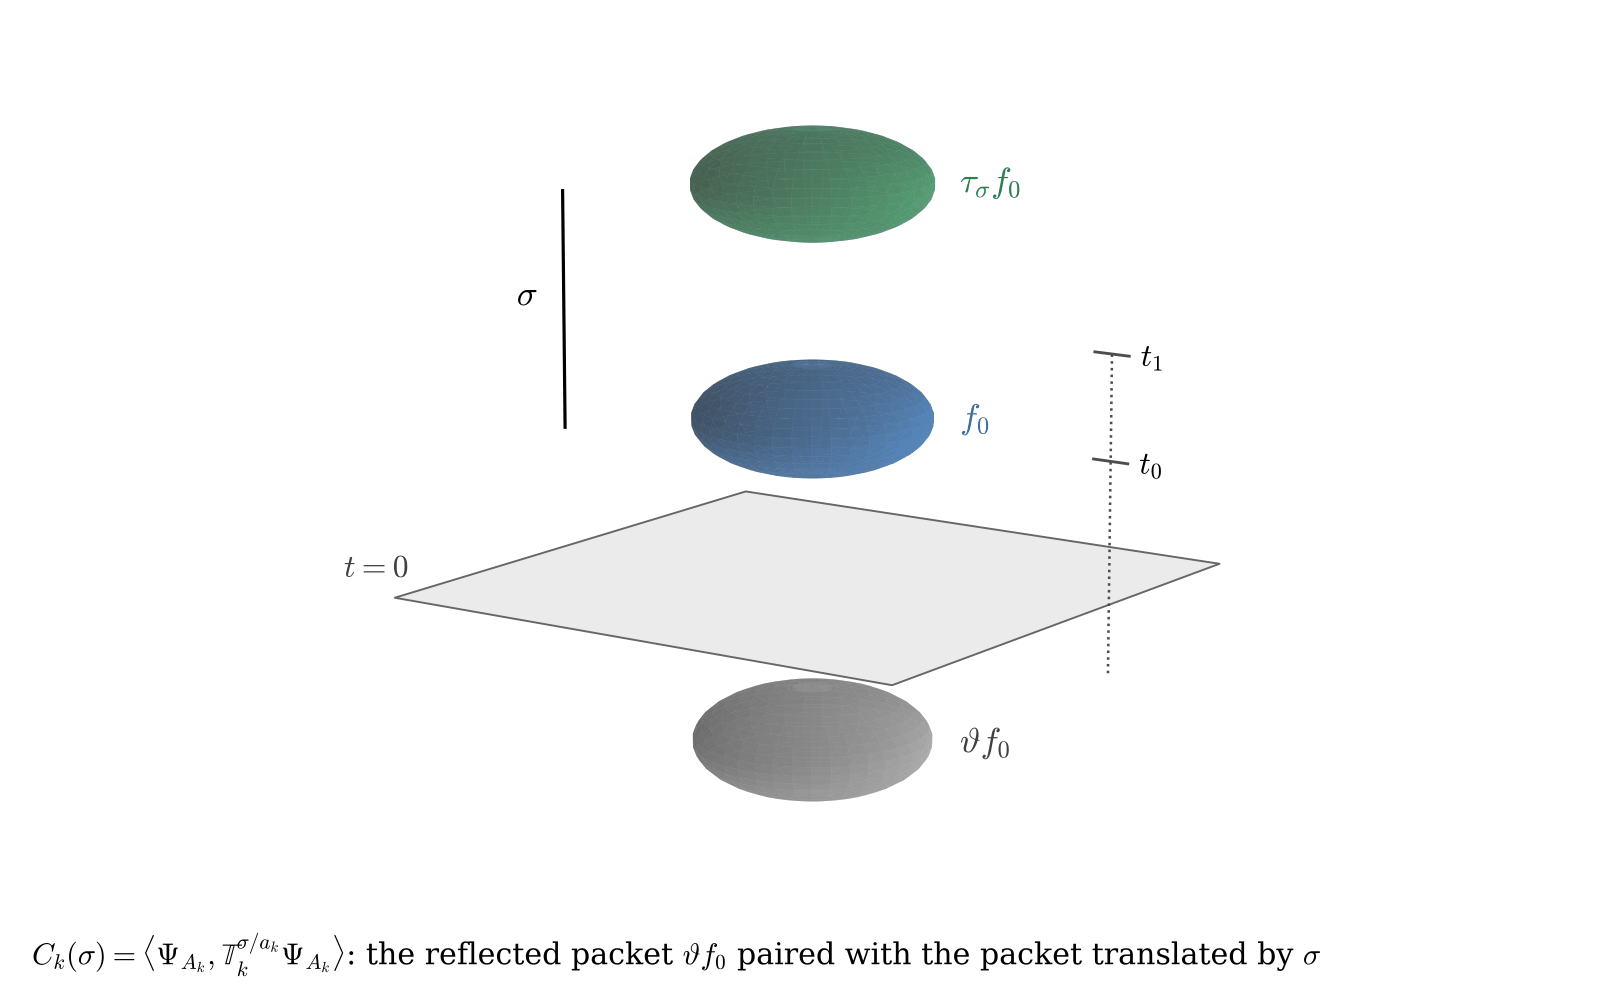
\includegraphics[width=0.82\textwidth]{figures/fig_packet.png}
\caption{The packet $f_0$ of Theorem~\ref{thm:flowlimit}, supported in the time
window $[t_0,t_1]$ above the reflection plane $t=0$, its reflection
$\vartheta f_0$ and its translate $\tau_\sigma f_0$ by $\sigma$ in time. The
correlation $C_k(\sigma)$ pairs the reflected packet with the translated one;
$C_k(0)$ is the reflected norm that renormalises the packet.}
\label{fig:packet}
\end{figure*}

\begin{theorem}\label{thm:flowlimit}
\textup{(i)} For $y,y'\in\mathcal D$ and every $k$ with $y/a_k,y'/a_k\in\Z^4$,
\[
Z_k^2\,\bigl|\omega_k\bigl(\vartheta(\bar A^y_k)A^{y'}_k\bigr)\bigr|\le1 .
\]
\textup{(ii)} Every sequence of $k$ has a subsequence along which
$K(y,y')=\lim Z_k^2\,\omega_k(\vartheta(\bar A^y_k)A^{y'}_k)$ exists for all
$y,y'\in\mathcal D$ and $\rho(\sigma)=\lim C_k(\sigma)/C_k(0)$ exists for all
dyadic $\sigma>0$. Along it there is a probability measure $\mu$ on $[0,\infty]$
with
\[
\rho(\sigma)=\int_{[0,\infty]}e^{-\sigma E}\,d\mu(E)\qquad(\sigma>0),
\]
the integrand being $0$ at $E=\infty$.

\textup{(iii)} Along such a subsequence, let $\mathcal T$ be spanned by the
translates $f_0(\cdot-y)$, $y\in\mathcal D$, and one more function $f_*\in
C_c(\R^4)$ supported in $\{t>0\}$ outside their span, and let $O_k$ be the
linear map with $O_k(f_0(\cdot-y))=Z_kA^y_k$ and $O_k(f_*)=1$. Then
$(\omega_k,O_k)$ has a continuum limit in the sense of
Definition~\ref{def:limit}, on which the dyadic spatial translations act by
unitary operators commuting with $H$.

\textup{(iv)} This limit is nontrivial if and only if $\mu([0,\infty))>0$, if and
only if $\rho(\sigma)>0$ for one dyadic $\sigma>0$, and then $\rho(\sigma)>0$
for all of them. Consequently a nontrivial limit exists along some subsequence
if and only if $\limsup_kC_k(\sigma)/C_k(0)>0$ for some dyadic $\sigma>0$.

\textup{(v)} If the hypothesis of Theorem~\ref{thm:transfer} holds, then $\mu$
is carried by $[m_*,\infty]$ and $\rho(\sigma)\le e^{-m_*\sigma}$.
\end{theorem}

\begin{proof}
By Proposition~\ref{prop:spatialflow}(ii) each $\Phi_x\circ\Phi_{s_k}$, and
hence each $A^y_k$, is a uniform limit of gauge-invariant local functions at
times $\ge1$, so the reconstruction of Appendix~\ref{app:transfer} applies to
them (its footnote). Write $\Psi_k=Z_k\Psi_{A_k}$. Since
$\ip{\Omega_k}{\Psi_{A_k}}=\omega_k(A_k)=0$ and $\|\Psi_k\|^2=Z_k^2C_k(0)=1$,
$\Psi_k$ is a unit vector orthogonal to $\Omega_k$. The relation
$\ip{\Psi_F}{\mathbb T_k^t\Psi_H}=\omega_k(\vartheta(\bar F)\tau_tH)$ for all $F$
gives $\Psi_{\tau_tH}=\mathbb T_k^t\Psi_H$. Spatial translations commute with
$\vartheta$ and with $\tau_t$ and leave $\omega_k$ invariant, so they act on the
reconstructed space by unitaries $U_k(x)$ that commute with $\mathbb T_k$.
Hence, for $y=(t,y')$,
\[
Z_k\Psi_{A^y_k}=U_k(y'/a_k)\,\mathbb T_k^{t/a_k}\Psi_k .
\]

(i) The left side of the inequality is $|\ip{Z_k\Psi_{A^y_k}}{Z_k
\Psi_{A^{y'}_k}}|\le1$, because $\|U_k\|=1$ and $0\le\mathbb T_k\le1$.

(ii) The set $\mathcal D\times\mathcal D$ is countable and the numbers are
bounded by (i), so a diagonal subsequence gives all the limits $K$; the limits
$\rho(\sigma)$ are among them, since $C_k(\sigma)/C_k(0)=
\ip{\Psi_k}{\mathbb T_k^{\sigma/a_k}\Psi_k}$ is the value of $K$ at
$y=y'=(\sigma/2,0)$. Let $\nu_k$ be the spectral measure (Lemma~\ref{lem:spectralmeasure}) of $\mathbb T_k$ at
$\Psi_k$, a probability measure on $[0,1]$, and $\mu_k$ its image under
$\lambda\mapsto-a_k^{-1}\log\lambda\in[0,\infty]$. Then
$C_k(\sigma)/C_k(0)=\int e^{-\sigma E}d\mu_k(E)$. The space $[0,\infty]$ is
compact, so a further subsequence has $\mu_k\to\mu$ weakly (Lemma~\ref{lem:helly}), and
$E\mapsto e^{-\sigma E}$ is continuous on $[0,\infty]$ for $\sigma>0$.

(iii) A finite combination $\sum_jc_jf_0(\cdot-y_j)$ with distinct $y_j$ that
vanishes has Fourier transform $\hat f_0(p)\sum_jc_je^{-ip\cdot y_j}=0$; since
$\hat f_0$ is analytic and not zero, the exponential sum vanishes on an open
set and every $c_j$ is zero. So the translates are linearly independent and
$O_k$ is well defined. On the space $V$ of finite sums $v=\sum_yc_y\delta_y$
over $\mathcal D$ put $B(v,w)=\sum\bar c_yc'_{y'}K(y,y')$. It is the limit of
$\ip{v_k}{w_k}$ with $v_k=\sum_yc_yZ_k\Psi_{A^y_k}$, hence positive
semidefinite; let $\mathcal H_0$ be the completion of $V$ modulo its null
space. For dyadic $\sigma\ge0$ and dyadic spatial $x$ define
$T(\sigma)\delta_y=\delta_{y+(\sigma,0)}$ and $U(x)\delta_y=\delta_{y+(0,x)}$.
At level $k$ these are $\mathbb T_k^{\sigma/a_k}$ and $U_k(x/a_k)$, so in the
limit $B(T(\sigma)v,w)=B(v,T(\sigma)w)$, $B(T(\sigma)v,T(\sigma)v)\le B(v,v)$,
$B(v,T(\sigma)v)\ge0$, and $U(x)$ preserves $B$. Thus $T(\sigma)$ extends to
commuting positive contractions on $\mathcal H_0$ with
$T(\sigma)T(\sigma')=T(\sigma+\sigma')$, and $U(x)$ to unitaries commuting with
them. For dyadic $\sigma>0$ the kernel of $T(\sigma)=T(\sigma/2)^2$ equals that
of $T(\sigma/2)$, so all these kernels coincide; and every $\delta_y$ with
$y=(t,y')$ equals $T(t/2)\delta_{(t/2,y')}$, a vector in the range of a
positive operator and so orthogonal to its kernel. Hence each $T(\sigma)$ is
injective on $\mathcal H_0$, and $H_0=-\log T(1)$ is a self-adjoint operator
with $H_0\ge0$ and $e^{-\sigma H_0}=T(\sigma)$ for dyadic $\sigma$, by the
uniqueness of positive roots. Put $\mathcal H=\C\Omega\oplus\mathcal H_0$,
$H=0\oplus H_0$, $\psi(f_0(\cdot-y))=\delta_y$ and $\psi(f_*)=\Omega$. The range
of $\psi$ is dense, and the identities of Definition~\ref{def:limit} hold: for
two translates they are the limits defining $K$, with $\tau_{\sigma/a_k}A^{y'}_k=
A^{y'+(\sigma,0)}_k$; and for $f_*$ they read $\omega_k(1)=1$ and
$\omega_k(\vartheta(\bar A^y_k))=\omega_k(\tau_{\sigma/a_k}A^y_k)=0$.

(iv) The limit is nontrivial exactly when $\mathcal H_0\ne0$, that is when
$\|\delta_y\|^2=K(y,y)=\rho(2t)$ is positive for some $y=(t,y')$. By (ii) and Lemma~\ref{lem:laplace}(b),
$\rho(\sigma)>0$ for one $\sigma>0$ if and only if $\mu([0,\infty))>0$, and
then $\rho(\sigma)>0$ for every $\sigma>0$. For the last statement choose a
subsequence along which $C_k(\sigma)/C_k(0)$ tends to its $\limsup$, and refine
it by (ii).

(v) Under that hypothesis the proof of Theorem~\ref{thm:transfer} gives
$\nu_k([0,e^{-\log(1/\alpha)/(2n_k)}])=1$ because $\Psi_k\perp\Omega_k$, so
$\mu_k$ is carried by $[\log(1/\alpha)/(2n_ka_k),\infty]\subset[m_*,\infty]$,
and so is the weak limit $\mu$.
\end{proof}

The measure $\mu$ is the spectral measure of the renormalised flowed field in
the limit: its part on $[0,\infty)$ is what survives as a state of the
continuum theory, and its atom at $\infty$ is the weight that the field puts on
energies that diverge in physical units. The theorem constructs the
renormalised continuum observables and their reconstruction for every tuning,
and it reduces their nontriviality to the lattice inequality
\[
\limsup_{k\to\infty}\frac{C_k(\sigma)}{C_k(0)}>0
\]
for one physical separation $\sigma$: the flowed two-point function of the
smeared packet at a fixed physical distance must not become negligible
against its reflected norm $C_k(0)$. If the lattice gap stayed above some $m>0$ in lattice units, the
ratio would be at most $e^{-m\sigma/a_k}$ and the limit would be trivial, so the
inequality is a condition on the tuning $\beta_k\to\infty$; it is not proved
here. Nor are the independence of the limit from the subsequence, Euclidean
invariance, or bounds on products of more than two renormalised fields, for
which (i) gives nothing because $Z_k$ may diverge (Theorem~\ref{thm:higher}
reduces them to tree bounds); (E) requires all of these.

The denominator $C_k(0)$ is the reflected norm of the packet smeared by
$f_0$, not a coincidence limit of point fields, and the distinction matters.
For the free massless scalar field in four dimensions with spatial momenta cut
off at $\Lambda$, the covariance at spatial separation $0$ is
$(1-(1+\Lambda t)e^{-\Lambda t})/(4\pi^2t^2)$ at time $t>0$ and
$\Lambda^2/(8\pi^2)$ at coincidence, so its ratio
$2(1-(1+\Lambda t)e^{-\Lambda t})/(\Lambda t)^2$ tends to zero as
$\Lambda\to\infty$, although the limiting field is the nontrivial Gaussian
field; for packets smeared by $f_0$ the reflected norms of that field have
finite positive limits and the ratio stays positive. The criterion of
Theorem~\ref{thm:flowlimit}(iv) is about the smeared packets $A_k$ only.

When the ratio is bounded below, renormalising at the separation $\sigma$
instead of $0$ removes the escape to infinite energy altogether, and one slab
of the transfer matrix gives a sufficient condition for the bound. Write
$\mu_k$ for the measures in the proof of Theorem~\ref{thm:flowlimit}.

\begin{proposition}\label{prop:flowshift}
\textup{(i)} Suppose $C_k(\sigma)\ge c\,C_k(0)$ for a dyadic $\sigma>0$, a
$c>0$ and every $k$ of a sequence. Let $\mu'_k$ be the spectral measure, in
energies $E=-a_k^{-1}\log\lambda$, of the unit vector
$C_k(\sigma)^{-1/2}\Psi_{A'_k}$ with $A'_k=\tau_{\sigma/2a_k}A_k$. Then
$\mu'_k$ is a probability measure on $[0,\infty)$,
\[
\mu'_k([\Lambda,\infty))\le c^{-1}e^{-\sigma\Lambda},\qquad
\int E^m\,d\mu'_k\le c^{-1}\Bigl(\frac m{e\sigma}\Bigr)^m ,
\]
and $t\mapsto C_k(\sigma+t)/C_k(\sigma)$ is Lipschitz on $[0,\infty)$ with
constant $(e\sigma c)^{-1}$. A subsequence of the $\mu'_k$ converges weakly to
a probability measure on $[0,\infty)$ with the same bounds.

\textup{(ii)} Suppose $\ip{\Psi_k}{(1-\mathbb T_k)\Psi_k}\le Ca_k$ for a
constant $C$ and every $k$ of a sequence. Then
$C_k(\sigma)/C_k(0)\ge e^{-2C\sigma}$ whenever $Ca_k\le\frac12$ and
$\sigma/a_k$ is an integer, and $\mu_k([\Lambda,\infty])\le C(a_k+\Lambda^{-1})$
for every $\Lambda>0$.
\end{proposition}

\begin{proof}
(i) We have $\Psi_{A'_k}=\mathbb T_k^{\sigma/2a_k}\Psi_{A_k}$, so the
measure $\mu'_k$ is $e^{-\sigma E}d\mu_k(E)$ divided by its mass
$C_k(\sigma)/C_k(0)\ge c$, and $e^{-\sigma E}$ vanishes at $E=\infty$. For
$E\ge\Lambda$ we have $e^{-\sigma E}\le e^{-\sigma\Lambda}$, and
$E^me^{-\sigma E}\le(m/e\sigma)^m$ for all $E\ge0$. The ratio in question is
the integral of $e^{-tE}$ against $\mu'_k$, and the inequality
$|e^{-tE}-e^{-sE}|\le|t-s|E$ with the moment bound for $m=1$ gives the
Lipschitz bound. The tail bound makes the sequence tight on
$[0,\infty)$, so Prokhorov's theorem gives the weak limit, and the bounds pass
to it because $\{E>\Lambda\}$ is open and $E^m$ is a monotone limit of bounded
continuous functions.

(ii) Let $\nu_k$ be the spectral measure of $\mathbb T_k$ at $\Psi_k$ on
$[0,1]$, a probability measure, and $n=\sigma/a_k$. By Jensen's inequality for
the convex function $\lambda^n$,
\[
\frac{C_k(\sigma)}{C_k(0)}=\int\lambda^nd\nu_k\ge\Bigl(\int\lambda\,d\nu_k
\Bigr)^n\ge(1-Ca_k)^n\ge e^{-2Ca_kn},
\]
since $\log(1-x)\ge-2x$ on $[0,\frac12]$. Moreover $Ca_k\ge\int(1-e^{-a_kE})
d\mu_k\ge(1-e^{-a_k\Lambda})\mu_k([\Lambda,\infty])$, and
$1-e^{-x}\ge x/(1+x)$.
\end{proof}

Part (ii) asks for an upper bound on a one-slab Dirichlet form, the opposite
direction to a mass gap, which bounds such forms from below. In the box of
Proposition~\ref{prop:flowpositive}, with $g$ smooth, the time smearing
supplies the factor $a_k$ up to one ratio: in the notation of its proof,
$\mathbb T_k=A$ and $\Psi_{A_k}=\sum_nw_n\mathbb T_k^nu$ with
$w_n=a_kg(a_kn)$ and $u=a_k^3F^c\psi_0$, and the identity $(1-\mathbb T_k)
\Psi_{A_k}=\sum_n(w_n-w_{n-1})\mathbb T_k^nu$ gives
$\ip{\Psi_k}{(1-\mathbb T_k)\Psi_k}\le a_k\|g'\|_{L^1}\|u\|/\|\Psi_{A_k}\|$, so
the hypothesis of (ii) holds when the vector $u$ of a single slice stays
comparable to the time-smeared packet. That comparison is not proved;
Proposition~\ref{prop:sliceratio} below bounds the ratio without it.

A one-slab bound of this kind also limits the mass that $D(n_k,\alpha)$
can supply. Let $e^{-m_k}$ be the norm of $\mathbb T_k$ on $\Omega_k^\perp$.
If a unit vector $\varphi_k\perp\Omega_k$ has $\ip{\varphi_k}{(1-\mathbb
T_k)\varphi_k}\le\kappa a_k<1$, then the spectral measure of $\mathbb T_k$
at $\varphi_k$ lives on $[0,e^{-m_k}]$, so $1-e^{-m_k}\le\kappa a_k$ and
$m_k\le-\log(1-\kappa a_k)$. If in addition $D(n_k,\alpha)$ holds with
$n_ka_k\le\ell$, Theorem~\ref{thm:onescale} gives $m_k\ge\log(1/\alpha)
/(2n_k)\ge a_k\log(1/\alpha)/(2\ell)$, and therefore
\[
\frac{\log(1/\alpha)}{2\ell}\le\frac{-\log(1-\kappa a_k)}{a_k}=\kappa+
O(a_k).
\]
So the physical mass $m_*$ of Theorem~\ref{thm:transfer} is at most the
constant $\kappa$ of any one-slab bound. The two hypotheses are compatible
because both are statements in physical units. The one-slab bound forces
$m_k\to0$, so it cannot come from an expansion whose convergence gives a
lattice gap bounded below in lattice units.


In a periodic spatial box the assumption $C_k(0)>0$ is a theorem. Let
$G=\SU(N)$ with its defining representation, and replace $\Z^4$ by
$\Z\times(\Z/L_k\Z)^3$ with $L_k\ge3$ and $\omega_k$ by the infinite-time
Wilson state of the box. The proof of Theorem~\ref{thm:flowlimit} uses only
reflection positivity and the transfer matrix once the spatial translations
are dropped, and parts (i)--(iv) hold in the box with $\mathcal D$ replaced by
its points $(t,0)$, the time translates of $f_0$ being independent by the
same Fourier argument in $t$.

\begin{proposition}\label{prop:flowpositive}
In the box, let $f_0(t,x)=g(t)h(x)$ with $g,h\ge0$, and let $\Phi=\sum_{i<j}
(N-\ReTr Q_{ij})$ be the energy of the three spatial plaquettes at the origin.
If $g(a_kn)h(a_kx)>0$ for some $n\ge1$ and some $x$, then $C_k(0)>0$.
\end{proposition}

\begin{proof}
L\"uscher proved that the transfer matrix is strictly positive~\cite{Lus77};
we recall the argument because the proof uses it in this form.

\emph{The one-link kernel.} Write $\chi$ for the character of the defining
representation and $b=\beta_W>0$. Then
\[
e^{\frac bN\operatorname{Re}\chi}=\sum_{m\ge0}\frac{(b/2N)^m}{m!}
(\chi+\bar\chi)^m ,
\]
and $(\chi+\bar\chi)^m$ is the character of $(\rho\oplus\bar\rho)^{\otimes m}$.
Every irreducible representation $\sigma$ occurs in one of these tensor
powers: their matrix coefficients span the algebra of polynomials in the
entries of $q$ and $\bar q$, which contains the constants and separates points,
so it is dense in $C(G)$ by the Stone--Weierstrass theorem, while the matrix
coefficients of a $\sigma$ that never occurred would be orthogonal to it by
Schur orthogonality. So the coefficient of every irreducible character in
$e^{\frac bN\operatorname{Re}\chi}$ is positive, and convolution with this
function acts on each isotypic part of $L^2(G)$ by a positive scalar.

\emph{The transfer matrix.} In the temporal gauge the transfer matrix of the
box acts on the gauge-invariant part of $L^2(G^{E})$, $E$ the spatial links
of one slice, as $M K M$, where $K$ is the tensor product over $E$ of the
convolutions above and $M$ is multiplication by the exponential of half the
spatial plaquette weight~\cite{Lus77,OSei78}. Both commute with gauge
transformations, $K$ is positive and injective by the first step, and $M$ is
positive and invertible, so $\ip v{MKMv}=\ip{Mv}{KMv}>0$ for $v\ne0$. Its
kernel is a continuous positive function, and $K$ is compact, so its largest eigenvalue $\lambda_0$ is
simple with an eigenfunction $\psi_0>0$, and with $A=MKM/\lambda_0$, a
function $F$ of the slice at time $n\ge0$ has $\Psi_F=A^nF\psi_0$ in the
reconstruction, $\Omega$ being $\psi_0$.

\emph{Conclusion.} Let $F=\sum_xh(a_kx)\,\Phi_x\circ\Phi_{s_k}$ and
$F^c=F-\omega_k(F)$. Then $\Psi_{A_k}=a_k^4\,p(A)F^c\psi_0$ with
$p(z)=\sum_{n\ge1}g(a_kn)z^n$, a polynomial with nonnegative coefficients,
not all zero, so $p>0$ on $(0,1]$ and $p(A)$ is injective. The function
$\sum_xh(a_kx)\Phi_x$ vanishes at the configuration with every link $1$ and is
positive at one with a single nontrivial link at a site where $h(a_kx)>0$; the
flow $\Phi_{s_k}$ is a bijection, so $F$ is not constant, and as $F$ is
continuous and $\psi_0>0$, $F^c\psi_0\ne0$. Hence $C_k(0)=\|\Psi_{A_k}\|^2>0$.
\end{proof}

The proposition removes the one assumption of Theorem~\ref{thm:flowlimit} in a
box; it says nothing about the ratio of part (iv), on which nontriviality
depends.

The ratio of Theorem~\ref{thm:flowlimit}(iv) can be compared with
correlations of a single slice field. Suppose that $f_0(t,x)=g(t)h(x)$ with
$g\ge0$ supported in $[t_0,t_1]$, $t_0<t_1$ positive and dyadic, let
\[
U_k=\sum_{x\in\Z^3}a_k^3h(a_kx)\bigl(\Phi_{(0,x)}\circ\Phi_{s_k}
-\omega_k(\Phi_{(0,x)}\circ\Phi_{s_k})\bigr)
\]
be the centred field of the slice at time $0$, smeared in space only, and put
$u_k=\Psi_{U_k}$ and
\[
D_k(r)=\ip{u_k}{\mathbb T_k^{r/a_k}u_k}
=\omega_k\bigl(\vartheta(\bar U_k)\,\tau_{r/a_k}U_k\bigr)
\]
for $r\in a_k\Z$, $r\ge0$. Let $n_0=\lceil t_0/a_k\rceil$ and
$n_1=\lfloor t_1/a_k\rfloor$.

\begin{proposition}\label{prop:sliceratio}
Assume $C_k(0)>0$, and let $\sigma\ge0$ with $\sigma/a_k\in\Z$.

\textup{(i)} $D_k(r)>0$ for every $r$, and
\[
\frac{D_k(2a_kn_1+\sigma)}{D_k(2a_kn_0)}\le\frac{C_k(\sigma)}{C_k(0)}\le
\frac{D_k(2a_kn_0+\sigma)}{D_k(2a_kn_1)} .
\]

\textup{(ii)} $\log D_k$ and $\log C_k$ are convex and nonincreasing on
$a_k\Z_{\ge0}$. If $D_k(r')\ge c\,D_k(r)$ with $r<r'$ and $c\le1$,
then $D_k(\beta)\ge c^{\max(1,(\beta-\alpha)/(r'-r))}D_k(\alpha)$ whenever
$r\le\alpha<\beta$; if $C_k(\sigma)\ge c\,C_k(0)$ with $\sigma>0$, then
$C_k(\sigma')\ge c^{\sigma'/\sigma}C_k(0)$ for $\sigma'\ge\sigma$.

\textup{(iii)} Let $k$ run through a sequence. If
$D_k(r')\ge c\,D_k(r)$ for dyadic $0<r<r'$ with $r\le2t_0$, a
$c\in(0,1]$ and every large $k$, then for every dyadic $\sigma\ge0$ and every
large $k$
\[
C_k(\sigma)\ge c^{\max(1,(2t_1-2t_0+\sigma)/(r'-r))}\,C_k(0).
\]
Conversely, if $C_k(\sigma)\ge c\,C_k(0)$ for a dyadic $\sigma>0$ and every
$k$, then $D_k(2t_0+\sigma')\ge c^{\sigma'/\sigma}D_k(2t_1)$ for every dyadic
$\sigma'\ge\sigma$ with $\sigma'>2(t_1-t_0)$ and every large $k$.
\end{proposition}

\begin{proof}
For a function $F$ of the slice at time $0$ and an integer $n\ge0$ we have
$\Psi_{\tau_nF}=\mathbb T_k^n\Psi_F$, since both have inner product
$\omega_k(\vartheta(\bar G)\tau_nF)$ with every $\Psi_G$. By time translation
invariance of $\omega_k$,
$A_k=\sum_nw_n\tau_nU_k$ with $w_n=a_kg(a_kn)\ge0$, and $w_n=0$ unless
$n_0\le n\le n_1$; so $\Psi_{A_k}=\sum_nw_n\mathbb T_k^nu_k$. Let $\nu$ be the
spectral measure of $\mathbb T_k$ at $u_k$, on $[0,1]$, and
$W(\lambda)=\sum_nw_n\lambda^n$. Then
\[
C_k(\sigma)=\int W(\lambda)^2\lambda^{\sigma/a_k}\,d\nu(\lambda),\qquad
D_k(r)=\int\lambda^{r/a_k}\,d\nu(\lambda).
\]

(i) Since $t_0>0$, $n_0\ge1$ and $W(0)=0$; so $C_k(0)>0$ forces $\nu((0,1])>0$, and then
$D_k(r)>0$. For $0\le\lambda\le1$,
$\|w\|_1\lambda^{n_1}\le W(\lambda)\le\|w\|_1\lambda^{n_0}$; inserting these
bounds in $C_k(\sigma)$ and $C_k(0)$ gives the two inequalities.

(ii) Convexity of $j\mapsto\log\int\lambda^j\,d\rho$ for a positive measure
$\rho$ on $[0,1]$ is H\"older's inequality, and the integrals decrease in $j$
because $\lambda\le1$; take $\rho=\nu$ and $\rho=W^2\nu$. If
$\beta\le r'$, monotonicity gives
$D_k(\beta)\ge D_k(r')\ge cD_k(r)\ge cD_k(\alpha)$. If $\beta>r'$, the
difference quotients of the convex function $\log D_k$ increase in both
end points, so $(\log D_k(\beta)-\log D_k(\alpha))/(\beta-\alpha)\ge
(\log D_k(r')-\log D_k(r))/(r'-r)\ge\log c/(r'-r)$. The
statement on $C_k$ is the same comparison of quotients on $[0,\sigma]$ and
$[0,\sigma']$.

(iii) For large $k$ the times $2t_0$, $2t_1$ are multiples of $a_k$, and
$2a_kn_0\ge2t_0$, $2a_kn_1\le2t_1$. Since $D_k$ is nonincreasing, (i) gives
\[
\frac{D_k(2t_1+\sigma)}{D_k(2t_0)}\le\frac{C_k(\sigma)}{C_k(0)}\le
\frac{D_k(2t_0+\sigma)}{D_k(2t_1)} .
\]
The first claim is the left inequality with (ii) for $\alpha=2t_0\ge r$ and
$\beta=2t_1+\sigma$. For the second, (ii) gives $C_k(\sigma')\ge
c^{\sigma'/\sigma}C_k(0)$, and the right inequality at $\sigma'$ gives the
claim, the two times being ordered because $\sigma'>2(t_1-t_0)$.
\end{proof}

So for the packet $g\otimes h$ the open input of
Theorem~\ref{thm:flowlimit}(iv) follows from an inequality between two
correlations of one slice field,
\[
\liminf_kD_k(r')/D_k(r)>0\quad\text{for one pair }0<r<r'\text{ with }r\le2t_0,
\]
and by (iii) a uniform bound for one packet gives one for every packet
$g'\otimes h$ with $g'$ supported in $[t_1,\infty)$. The condition $r\le2t_0$
cannot be dropped: a bound at a later pair says nothing about an earlier
packet, as $D_k(r)=(1-4^{-k})2^{-kr}+4^{-k}2^{-r}$ shows, with
$D_k(4)/D_k(3)\to\frac12$ and $D_k(2)/D_k(1)\to0$. A bound at a later pair
does apply to the packet shifted forward in time, renormalised by its own
reflected norm. The left inequality of
(i) bounds the ratio without the comparison of $u$ with the packet that was
needed after Proposition~\ref{prop:flowshift}(ii). Every bound on such ratios
proved in this paper, at strong coupling or through
Theorem~\ref{thm:transfer}, is an upper bound of the form
$e^{-m(r'-r)/a_k}$; the inequality above is the opposite one and says
that the slice field does not put its weight on energies that diverge in
physical units. Reflection positivity and positivity of the transfer matrix
do not give it, since a lattice theory with a fixed mass in lattice units has
both and its ratio tends to zero. It holds for the free field.

\begin{remark}\label{rem:freeslice}
Let $D_k$ be defined as above for the massless free lattice field on
$a_k\Z^4$ in place of $\Phi$, with $h\in C^\infty_c(\R^3)$ and the lattice heat
flow for a physical time $t_f>0$ in place of the gradient flow. With $\hat p^2=\sum_i(2a_k^{-1}\sin
(a_kp_i/2))^2$, $\cosh(a_k\omega)=1+a_k^2\hat p^2/2$ and
$\hat h_k(p)=\sum_xa_k^3h(a_kx)e^{-ia_kp\cdot x}$,
\[
D_k(r)=\int_{[-\pi/a_k,\pi/a_k]^3}|\hat h_k(p)|^2e^{-2t_f\hat p^2}
\frac{e^{-r\omega}}{2a_k^{-1}\sinh(a_k\omega)}\,\frac{d^3p}{(2\pi)^3} .
\]
On the Brillouin zone $\hat p\ge2|p|/\pi$ and $a_k^2\hat p^2/2\le6$; as
$\operatorname{arccosh}(1+y)/\sqrt{2y}$ decreases on $(0,6]$, $a_k\omega\ge
\kappa a_k\hat p$ with $\kappa=\operatorname{arccosh}7/\sqrt{12}>0.76$, and
$a_k^{-1}\sinh(a_k\omega)\ge\omega$. Since $|\hat h_k|$ is bounded
uniformly in $k$, the integrands are dominated by a multiple of
$e^{-8t_f|p|^2/\pi^2}/|p|$, which is integrable on $\R^3$, and they
converge pointwise to $|\hat h(p)|^2e^{-2t_f|p|^2}e^{-r|p|}/
(2|p|)$. By dominated convergence $D_k(r')/D_k(r)$ tends to the
corresponding positive ratio of continuum integrals; for $h=e^{-|x|^2}$,
$t_f=0.05$, $r=\frac12$ and $r'=1$ it is $0.6337$.
\end{remark}

\begin{remark}\label{rem:twodslice}
The inequality also holds along the right tuning in two-dimensional $\SU(N)$
lattice gauge theory, which is interacting and nonabelian but has no
propagating gluons. Take the lattice $a_k\Z\times a_k\Z_{L_k}$ with
$a_kL_k=\ell$ fixed, the weight $\prod_p\exp(\frac{\beta_k}N\ReTr U_p)$ with
$\beta_k=2N/(g^2a_k^2)$, and the temporal gauge. A gauge-invariant function
of the links of one slice depends only on the conjugacy class of their
holonomy $V$ around the circle; this includes every spatially flowed and
spatially smeared slice field, since the flow is gauge covariant. Let
$w_\beta$ be the probability density proportional to
$e^{\frac\beta N\ReTr U}$ with respect to Haar measure and, for an irreducible
representation $\lambda$ of dimension $d_\lambda$ and character
$\chi_\lambda$, $\hat c_\lambda(\beta)=d_\lambda^{-1}\int\chi_\lambda
w_\beta\,dU$. Between two slices put $W_x=V'_xV_x^{-1}$; the $W_x$ are
independent with density $w_{\beta_k}$, which is invariant under conjugation
and inversion, and
\[
\begin{split}
V'_1\cdots V'_{L}&=W_1\,(V_1W_2V_1^{-1})\cdots\\
&\quad\cdots(V_1\cdots V_{L-1}W_{L}(V_1\cdots V_{L-1})^{-1})\,V_1\cdots V_{L},
\end{split}
\]
so the new holonomy is $QV$ with $Q$ distributed as the $L_k$-fold
convolution of $w_{\beta_k}$, independent of $V$. By Schur's lemma (Lemma~\ref{lem:convolution}) the
transfer matrix acts on class functions by $\chi_\lambda\mapsto\hat
c_\lambda(\beta_k)^{L_k}\chi_\lambda$. The coefficients are real, since
$w_\beta$ is invariant under $U\mapsto\bar U$, nonnegative, since the
exponential of $\frac\beta{2N}(\chi_{\mathrm F}+\bar\chi_{\mathrm F})$ is a sum of
characters with nonnegative coefficients, and below $1$ for
$\lambda\ne0$. For a class function $f$ with $\int f\,dU=0$ and isotypic
components of norms $|\hat f_\lambda|$, the slice correlation is therefore
\[
D_k(r)=\sum_{\lambda\ne0}|\hat f_\lambda|^2e^{-rE_{\lambda,k}},\qquad
E_{\lambda,k}=-\frac{\ell}{a_k^2}\log\hat c_\lambda(\beta_k).
\]
Laplace's method\footnote{For a smooth function with a unique nondegenerate maximum, $\int e^{\beta\varphi}h$ has an expansion in powers of $\beta^{-1}$ whose coefficients are Gaussian moments at the maximum; Lemma~\ref{lem:wilsoncoeff} carries it out here.} at the unique maximum $U=1$ of $\ReTr U$, with
$U=e^X$, $\ReTr e^X=N+\frac12\operatorname{Tr}X^2+O(|X|^4)$,
$\operatorname{Re}\operatorname{Tr}X^3=0$, $\operatorname{Tr}\rho_\lambda(X)=0$
and $\sum_a\rho_\lambda(T_a)^2=-2C_2(\lambda)$ for an orthonormal basis of
$\mathfrak{su}(N)$ in the norm $-\operatorname{Tr}X^2$, gives $\hat
c_\lambda(\beta)=1-NC_2(\lambda)/\beta+O(\beta^{-2})$, with the Casimir
normalised by $C_2=(N^2-1)/(2N)$ on the fundamental representation (Lemma~\ref{lem:wilsoncoeff}). Hence
$E_{\lambda,k}\to g^2\ell C_2(\lambda)/2$, and since $D_k(r)\le\|f\|^2$,
\[
\liminf_k\frac{D_k(r')}{D_k(r)}\ge\frac{|\hat f_\mu|^2}{\|f\|^2}
e^{-r'g^2\ell C_2(\mu)/2}>0
\]
for every $\mu\ne0$ with $\hat f_\mu\ne0$; for $f=\ReTr V$ the ratio is
exactly $e^{-(r'-r)E_{\mathrm F,k}}\to e^{-(r'-r)g^2\ell(N^2-1)/(4N)}$. This
is the exact solution of two-dimensional lattice gauge theory, whose
continuum limit is the measure of~\cite{GKS89,Dri89,Lev03}, written as
the inequality. In two dimensions $g^2$ has the dimension of a mass squared
and there is no ultraviolet problem, so the argument has no four-dimensional
analogue. Nor does the spatial flow give the inequality by itself: it damps
the spectral weight at large spatial momentum and leaves the weight at zero
spatial momentum unchanged. For the free lattice field of
Remark~\ref{rem:freeslice} with a mass $M_k$ and the same flow, every energy
is at least $m_k=a_k^{-1}\operatorname{arccosh}(1+a_k^2M_k^2/2)$, so
$D_k(r')\le e^{-m_k(r'-r)}D_k(r)$, which tends to zero relative to $D_k(r)$
when $a_kM_k$ is fixed.
\end{remark}

\begin{figure*}[t]
\centering
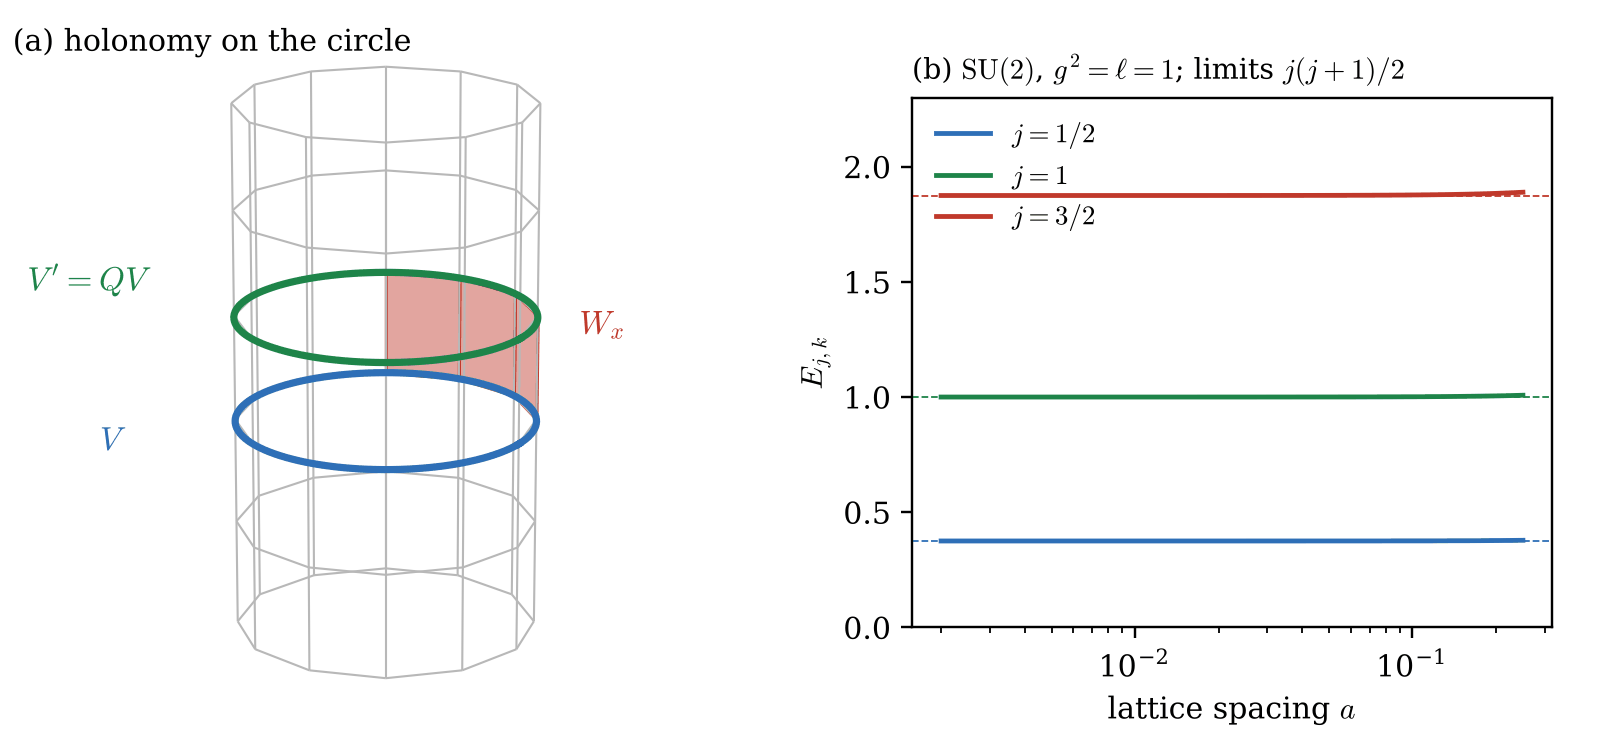
\includegraphics[width=0.9\textwidth]{figures/fig_twod.png}
\caption{Two-dimensional $\SU(N)$ (Remark~\ref{rem:twodslice}). (a) The lattice
$a_k\Z\times a_k\Z_{L_k}$ drawn as a cylinder: the holonomy $V$ of one slice,
the holonomy $V'=QV$ of the next, and the plaquette variables $W_x$ between
them. (b) The energies $E_{j,k}=-(\ell/a_k^2)\log\hat c_j(\beta_k)$ of
$\SU(2)$ for $g^2=\ell=1$, with $\hat c_j(\beta)=I_{2j+1}(\beta)/I_1(\beta)$,
against the lattice spacing; the dashed lines are the limits $j(j+1)/2$.}
\label{fig:twod}
\end{figure*}

\begin{figure*}[t]
\centering
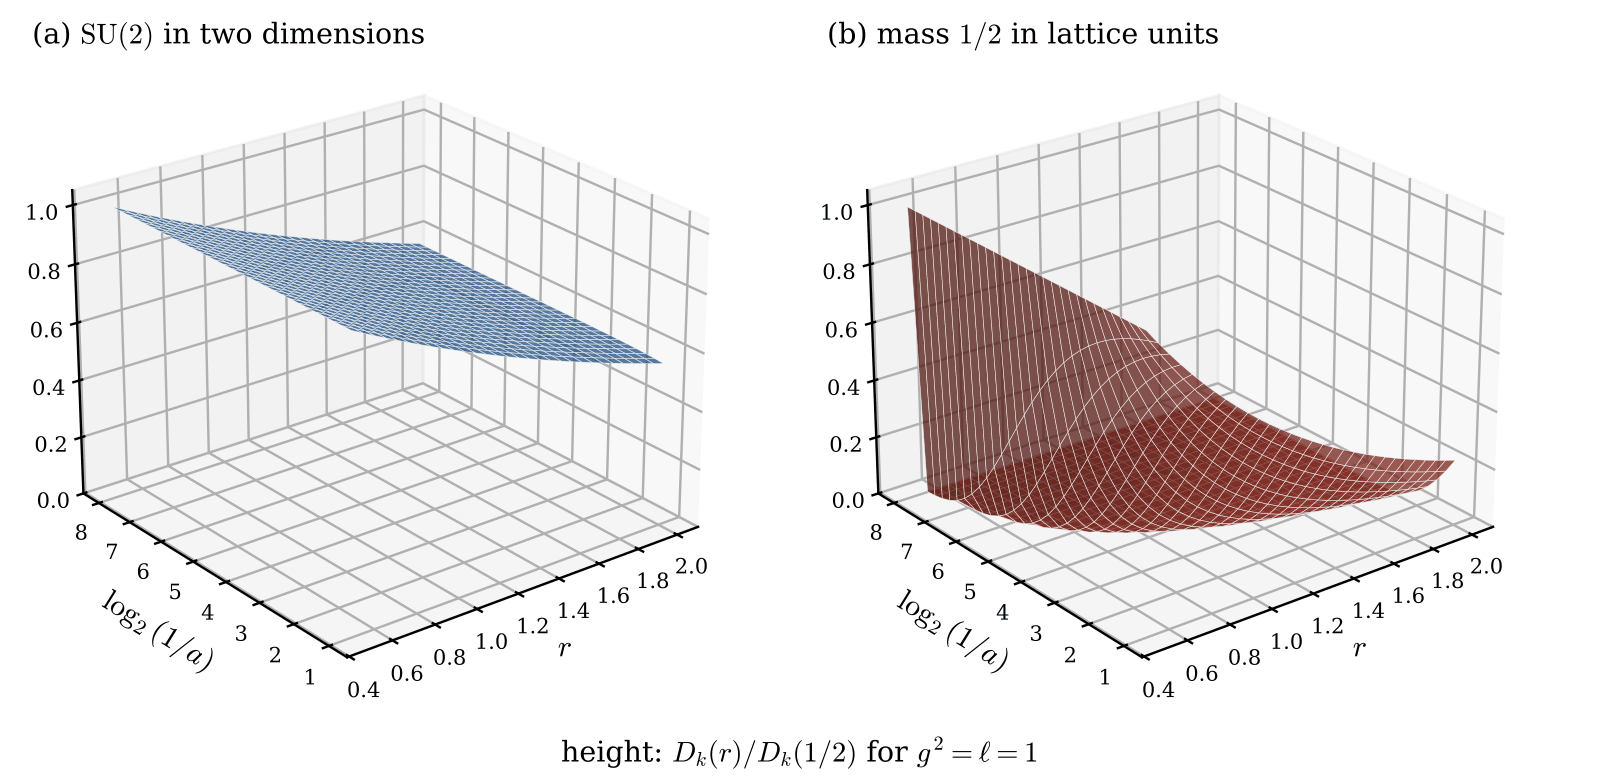
\includegraphics[width=0.9\textwidth]{figures/fig_slice.png}
\caption{The ratio $D_k(r)/D_k(\frac12)$ over the separation $r$ and the lattice
spacing $a_k$. (a) Two-dimensional $\SU(2)$ with $f=\ReTr V$ and
$g^2=\ell=1$, where the ratio is $e^{-(r-1/2)E_{1/2,k}}$ and converges as
$a_k\to0$. (b) The term $e^{-(r-1/2)m_k}$ of the lowest energy $m_k$ of a free
field with mass $\frac12$ in lattice units, which bounds the ratio from above
and tends to zero at every $r>\frac12$.}
\label{fig:slice}
\end{figure*}

A route to the slice ratio in four dimensions replaces the packet by its
conditional expectations given averages of the field over blocks of
increasing size and controls the error of each step. The free field shows in
which norm such errors can be small. In the ordinary $L^2$ norm the first
step already fails: conditioning on the averages over blocks of side two
leaves a fixed fraction of the variance of an energy packet, at every
lattice spacing.

\begin{proposition}\label{prop:blockfree}
Let $d\ge2$, let $\Lambda$ be a periodic box in $\Z^d$ with even sides, let
$\mu>0$, and let $\phi$ be the Gaussian field on $\Lambda$ with density
proportional to
$\exp\bigl(-\frac12\sum_{x,\nu}(\nabla_\nu\phi(x))^2-\frac{\mu^2}2\sum_x
\phi(x)^2\bigr)$, where $\nabla_\nu\phi(x)=\phi(x+e_\nu)-\phi(x)$. Let
$\mathcal Z$ be a set of blocks $B=2z+\{0,1\}^d$, let $\mathfrak B$ be the
$\sigma$-algebra generated by the averages of $\phi$ over the blocks in
$\mathcal Z$, let $f\ge0$ on $\Lambda$, and let
\[
F=\sum_{x\in\Lambda}f(x)\sum_{\nu=1}^d{:}(\nabla_\nu\phi(x))^2{:} ,
\]
where ${:}X^2{:}=X^2-\E X^2$. For $B=2z+\{0,1\}^d$ put $x_B=2z$,
$y_B=2z+e_1+e_2$ and
\[
\alpha_B=\frac14\sum_{w\in\{x_B,y_B\}}\Bigl(d\,f(w)+\sum_{\nu=1}^df(w-e_\nu)
\Bigr),
\]
and $\sigma^2=2/(2d+\mu^2)$.
\textup{(i)} $\E\Var(F\mid\mathfrak B)\ge2\sigma^4\sum_{B\in\mathcal Z}\alpha_B^2$.

\textup{(ii)} $\Var F\le2d^2\sum_xf(x)^2$.

\textup{(iii)} Let $g\ge0$ be a Lipschitz function on $\R^d$ with compact
support and $\int g^2>0$. For $n\ge1$ let $\Lambda_n$ contain $n\operatorname{supp}g$
in a fundamental domain, $f_n(x)=g(x/n)$, let $\mathcal Z_n$ contain every
block that meets $n\operatorname{supp}g$, and let $\mu=\mu_n\to0$. Then for
the packets $F_n$ of $f_n$,
\[
\liminf_{n\to\infty}\frac{\E\Var(F_n\mid\mathfrak B_n)}{n^d\int g^2}
\ge2^{1-d},\qquad
\limsup_{n\to\infty}\frac{\Var F_n}{n^d\int g^2}\le2d^2 ,
\]
so $\E\Var(F_n\mid\mathfrak B_n)\ge(2^{-d}d^{-2}-o(1))\Var F_n$.
\end{proposition}

\begin{proof}
(i) No two of the sites $x_B,y_B$, $B\in\mathcal Z$, are neighbours: their
coordinate sums are even, and a neighbour of a site has a coordinate sum of
the other parity. Let $\mathfrak H\supseteq\mathfrak B$ be generated by
$\mathfrak B$ and by $\phi(w)$ for every $w$ outside
$\{x_B,y_B:B\in\mathcal Z\}$. By the law of total variance,
$\Var(F\mid\mathfrak B)=\E[\Var(F\mid\mathfrak H)\mid\mathfrak B]
+\Var(\E[F\mid\mathfrak H]\mid\mathfrak B)$, so
$\E\Var(F\mid\mathfrak B)\ge\E\Var(F\mid\mathfrak H)$. In the exponent of the
density, a site $w$ enters through $(d+\frac{\mu^2}2)\phi(w)^2$ and through
$-\phi(w)\phi(w')$ for each of its $2d$ neighbours $w'$. Given $\mathfrak H$,
the block average fixes $s_B=\phi(x_B)+\phi(y_B)$, and with
$u_B=\phi(x_B)-\phi(y_B)$ we have $\phi(x_B)^2+\phi(y_B)^2=\frac12(s_B^2+
u_B^2)$. Since the free sites have only $\mathfrak H$-measurable neighbours,
the conditional density of $(u_B)_{B\in\mathcal Z}$ is proportional to
$\prod_B\exp(-\frac14(2d+\mu^2)u_B^2+c_Bu_B)$ with $\mathfrak H$-measurable
$c_B$: the $u_B$ are conditionally independent Gaussians of variance
$\sigma^2$. A term $(\nabla_\nu\phi(w))^2$ contains at most one free site,
and if it contains $x_B$, then $\phi(x_B)=\frac12(s_B+u_B)$ shows that it is
$\frac14u_B^2$ plus a term linear in $u_B$ plus an $\mathfrak
H$-measurable term; the same holds for $y_B$ with $-u_B$. The terms
containing $x_B$ are those with $w=x_B$ and those with $w=x_B-e_\nu$, $d$ of
each kind, so
\[
F=\sum_{B\in\mathcal Z}\bigl(\alpha_Bu_B^2+\beta_Bu_B\bigr)+F_0
\]
with $\mathfrak H$-measurable $\beta_B$ and $F_0$. Writing
$u_B=m_B+v_B$ with $m_B$ the conditional mean, $\alpha_Bu_B^2+\beta_Bu_B=
\alpha_Bv_B^2+(2\alpha_Bm_B+\beta_B)v_B+\text{const}$, and for a centred
Gaussian $v$ of variance $\sigma^2$, $\Var(\alpha v^2+\gamma v)=2\alpha^2
\sigma^4+\gamma^2\sigma^2$. By conditional independence,
$\Var(F\mid\mathfrak H)\ge2\sigma^4\sum_B\alpha_B^2$.

(ii) For centred jointly Gaussian $X,Y$, $\Cov({:}X^2{:},{:}Y^2{:})=2\Cov(X,Y)^2$.
With $G_{\nu\rho}(x,y)=\E[\nabla_\nu\phi(x)\nabla_\rho\phi(y)]$,
\[
\begin{split}
\Var F&=2\sum_{x,y}f(x)f(y)\sum_{\nu,\rho}G_{\nu\rho}(x,y)^2\\
&\le\sum_{x,y}\bigl(f(x)^2+f(y)^2\bigr)\sum_{\nu,\rho}G_{\nu\rho}(x,y)^2 .
\end{split}
\]
On the dual torus $\Lambda^*$, with $\hat p^2=\sum_\nu|e^{ip_\nu}-1|^2$,
\[
G_{\nu\rho}(x,y)=\frac1{|\Lambda|}\sum_{p\in\Lambda^*}
\frac{(e^{ip_\nu}-1)(e^{-ip_\rho}-1)}{\hat p^2+\mu^2}e^{ip\cdot(x-y)},
\]
and by Parseval
$\sum_yG_{\nu\rho}(x,y)^2=|\Lambda|^{-1}\sum_p|e^{ip_\nu}-1|^2
|e^{ip_\rho}-1|^2(\hat p^2+\mu^2)^{-2}\le1$, since each factor
$|e^{ip_\nu}-1|^2$ is at most $\hat p^2$. The same holds for the sum over
$x$, and (ii) follows.

(iii) If $\operatorname{Lip}g=K$, every site entering $\alpha_B$ lies within
distance $3$ of $2z$, so $|\alpha_B-d\,g(2z/n)|\le3dK/n$. Hence
$\sum_{B\in\mathcal Z_n}\alpha_B^2\ge\sum_z(d\,g(2z/n)-3dK/n)_+^2$, the sum
running over $z$ with $2z\in n\operatorname{supp}g$, and this is
$d^2(n/2)^d\int g^2\,(1+o(1))$ as a Riemann sum on the grid $(2/n)\Z^d$.
Since $\sigma^4=4/(2d+\mu_n^2)^2\to d^{-2}$, (i) gives the first bound. By
(ii) and $\sum_xg(x/n)^2=n^d\int g^2(1+o(1))$, the second follows.
\end{proof}

For $d=4$ and the energy density, $\Var F_n$ grows like $(\ell/a)^4$ at a
fixed physical size $\ell$ of the packet, and no step of conditioning on
block averages removes more than a fraction $1-2^{-d}d^{-2}+o(1)$ of it. The
reflected norm $C_k(0)=\omega_k(\vartheta(\bar A_k)A_k)$, which renormalises
the packet in Theorem~\ref{thm:flowlimit}, involves the covariance only
between the support of $\vartheta f_0$ and that of $f_0$, at a fixed
physical distance. The errors of a blocking route have therefore to be
measured in that norm; Figure~\ref{fig:blocking} shows the blocks between
the reflection plane and the packet.

\begin{figure*}[t]
\centering
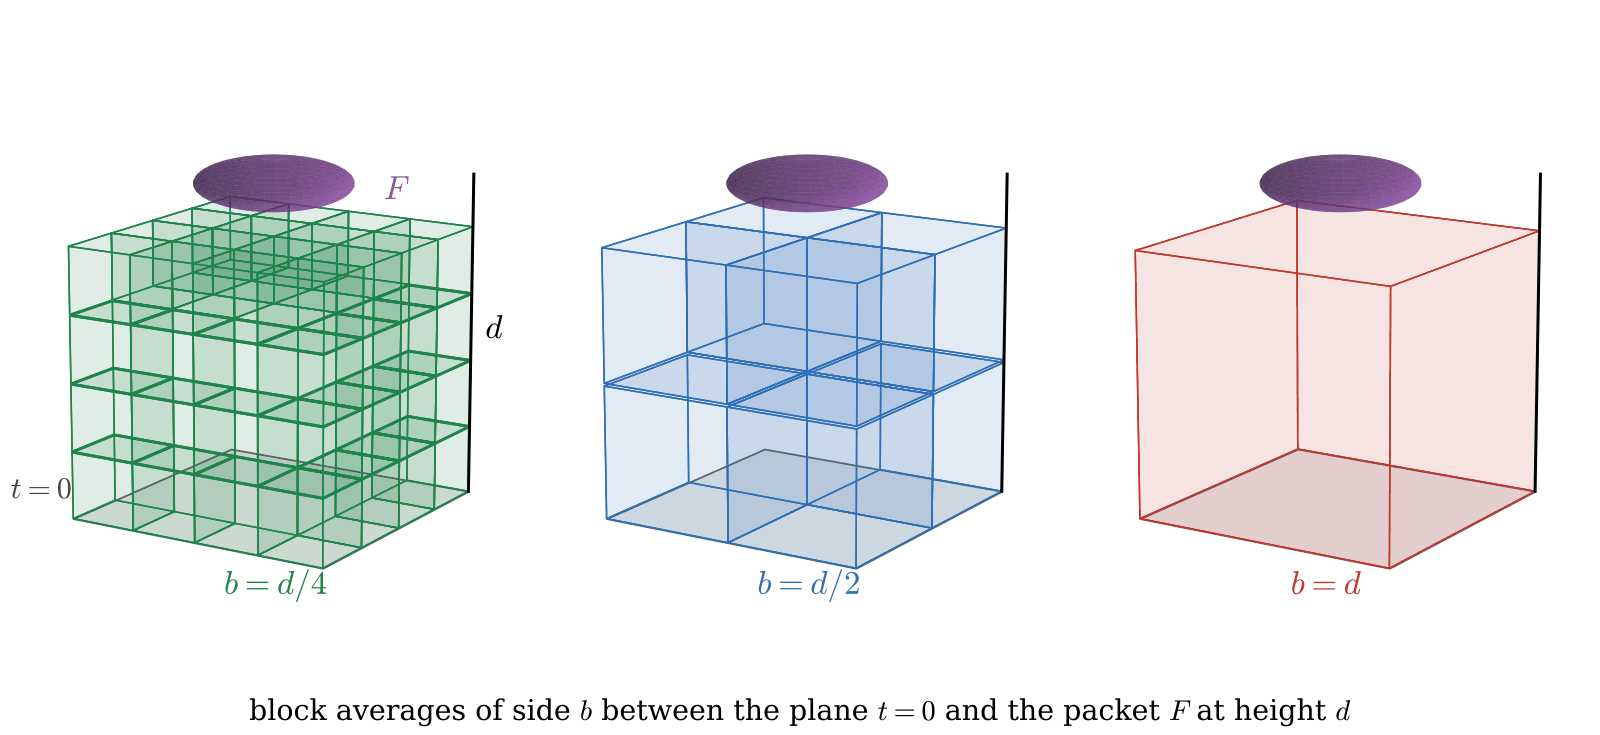
\includegraphics[width=0.9\textwidth]{figures/fig_blocking.png}
\caption{Block averages between the reflection plane $t=0$ and a packet $F$ at
physical height $d$, for blocks of side $d/4$, $d/2$ and $d$. By
Proposition~\ref{prop:blockfree} the first conditioning step already leaves
a fixed fraction of the ordinary variance of the packet, so the errors of
such steps have to be measured in the reflected norm.}
\label{fig:blocking}
\end{figure*}


\subsection{Higher correlations}\label{ssec:higher}

Theorem~\ref{thm:flowlimit} controls two renormalised fields at a time, and
part (i) of it gives nothing for more: $Z_k$ may diverge while the fields
$\Phi_x\circ\Phi_{s_k}$ stay bounded, so a bound on the norm of the
renormalised packet as an operator is not available. A reflection positive
process with a fixed gap and a two-point function independent of the
cutoff can have divergent four-point functions at separated times
(Remark~\ref{rem:markov}), so no statement about the two-point function alone
can replace the following hypothesis on the truncated correlations. In this
subsection $\Phi$ is real-valued, as the energy of the plaquettes is; for a
complex field the conjugate field has to be adjoined and (T1) imposed on all
mixed cumulants. Write $\varphi_k(x)=\Phi_x\circ\Phi_{s_k}$,
$\omega^T_k$ for the truncated correlations (joint cumulants) under
$\omega_k$, and for $f\in C_c(\R^4)$
\[
A_k(f)=\sum_{x\in\Z^4}a_k^4f(a_kx)\bigl(\varphi_k(x)-\omega_k(\varphi_k(x))\bigr),
\]
so that $A_k=A_k(f_0)$ and $\bar A_k(f)=A_k(\bar f)$. Let
$w_k:\Z^4\to[0,\infty)$ be even functions with $W_k=\sum_xw_k(x)<\infty$, let
$r_k>0$ be amplitude scales, and consider:
\begin{enumerate}[label=\textup{(T\arabic*)},leftmargin=*]
\item \emph{Tree bounds.} For every $n\ge2$ there is $K_n$, independent of $k$,
with
\[
\bigl|\omega^T_k\bigl(\varphi_k(x_1);\dots;\varphi_k(x_n)\bigr)\bigr|
\le K_nr_k^n\sum_{T}\prod_{\{i,j\}\in T}w_k(x_i-x_j)
\]
for all $x_1,\dots,x_n\in\Z^4$, the sum running over the trees $T$ on
$\{1,\dots,n\}$.
\item \emph{Saturation.} $C_k(0)\ge c\,r_k^2a_k^4W_k$ for a $c>0$ and every $k$.
\item \emph{Physical volume.} $B_*=\sup_ka_k^4W_k<\infty$.
\end{enumerate}
The amplitude $r_k$ separates the size of the field from the volume over
which it is correlated; Remark~\ref{rem:amplitude} shows why it is needed.
For a compact $Q\subset\R^4$ let $|Q|_k=a_k^4\,\#\{x\in\Z^4:a_kx\in Q\}$; for a
cube of side $L$ it is at most $(L+a_0)^4$.

\begin{lemma}\label{lem:treesum}
Under \textup{(T1)}, for $n\ge2$ and bounded $f_1,\dots,f_n$ with compact
supports, $f_1$ supported in $Q$,
\[
\begin{split}
&\bigl|\omega^T_k\bigl(A_k(f_1);\dots;A_k(f_n)\bigr)\bigr|\\
&\qquad\le K_nn^{n-2}r_k^n\,|Q|_k\,(a_k^4W_k)^{n-1}\prod_{j=1}^n\|f_j\|_\infty .
\end{split}
\]
\end{lemma}

\begin{proof}
Joint cumulants of order $n\ge2$ are multilinear and do not change when
constants are added to the variables, so the left side is at most
$a_k^{4n}\sum_{x_1,\dots,x_n}\prod_j|f_j(a_kx_j)|$ times the absolute value
of the truncated correlation, the sums being finite. Insert (T1) and fix a
tree $T$. With $x_1$ fixed, sum over the other points one at a time, each
time over a leaf of what remains of $T$ other than $1$; each such sum is at
most $W_k$. The remaining sum over $x_1$ has at most $|Q|_ka_k^{-4}$ nonzero
terms. There are $n^{n-2}$ trees.
\end{proof}

\begin{theorem}\label{thm:higher}
Assume \textup{(T1)--(T3)}.

\textup{(i)} For $n\ge2$, $f_j$ as in the lemma,
\[
\begin{split}
&\bigl|\omega^T_k\bigl(Z_kA_k(f_1);\dots;Z_kA_k(f_n)\bigr)\bigr|\\
&\qquad\le K_nn^{n-2}c^{-n/2}\,B_*^{\,n/2-1}\,|Q|_k\prod_{j=1}^n\|f_j\|_\infty ,
\end{split}
\]
and the moments $\omega_k\bigl(\prod_jZ_kA_k(f_j)\bigr)$ with all
$f_j$ supported in a cube $Q$ are bounded by $M_n(Q)\prod_j\|f_j\|_\infty$,
with $M_n(Q)$ independent of $k$.

\textup{(ii)} Every sequence of $k$ has a subsequence along which
\[
S_n(f_1,\dots,f_n)=\lim_k\omega_k\Bigl(\prod_{j=1}^nZ_kA_k(f_j)\Bigr)
\]
exists for all $n$ and all $f_j\in C_c(\R^4)$. Each $S_n$ is symmetric,
multilinear, bounded by $M_n(Q)\prod_j\|f_j\|_\infty$ on functions supported in
$Q$, hence a distribution on $(\R^4)^n$; it is invariant under all
translations of $\R^4$ if the $\omega_k$ are translation invariant, and the
kernel $K$ of Theorem~\textup{\ref{thm:flowlimit}} along the subsequence is
$K(y,y')=S_2\bigl(\overline{f_0(\cdot-y)}\circ\theta,f_0(\cdot-y')\bigr)$, with
$\theta$ as in \textup{(iii)}.

\textup{(iii)} Put $S_0=1$, $S_1=0$, and let $\theta$ be the reflection
$t\mapsto-t$ of $\R^4$. For every finite family of $c_\alpha\in\C$ and
$f_{\alpha,j}\in C_c(\R^4)$ supported in $\{t>0\}$,
\[
\sum_{\alpha,\beta}\bar c_\alpha c_\beta\,
S\Bigl(\prod_j\overline{f_{\alpha,j}}\circ\theta\cdot\prod_jf_{\beta,j}\Bigr)\ge0,
\]
where $S$ of a product of $n$ test functions means $S_n$. Hence the
Osterwalder--Schrader construction gives a Hilbert space $\mathcal H$ with
vacuum $\Omega$ and a dense set of vectors $\Psi(P)$ indexed by polynomials $P$
in the smeared fields at positive times, with
$\ip{\Psi(P)}{\Psi(P')}=S(\theta\bar P\cdot P')$; in particular the separated
higher correlations of the renormalised fields are finite. The vector
$\Psi(P_0)$ of the field smeared by $f_0$ is a unit vector orthogonal to
$\Omega$.

\textup{(iv)} Suppose the $\omega_k$ are translation invariant. Then the
time translations by $t\ge0$ define on $\mathcal H$ a strongly continuous
semigroup $e^{-tH}$ with $H\ge0$ self-adjoint, and the spatial translations a
strongly continuous unitary group commuting with $H$. Moreover there is a
dyadic $\sigma>0$ with $C_k(\sigma)\ge\frac12C_k(0)$ for all large $k$, so
the limit of Theorem~\textup{\ref{thm:flowlimit}} is nontrivial.

\textup{(v)} If $a_k^4W_k\to0$ along the subsequence, every $S_n$ is given by
Wick's rule from $S_2$: the limit is the Gaussian field with covariance $S_2$.

\textup{(vi)} If the $\omega_k$ are translation invariant and the
hypothesis of Theorem~\textup{\ref{thm:transfer}} holds, then $0$ is a simple
eigenvalue of $H$ and $\sigma(H)\subset\{0\}\cup[m_*,\infty)$ with
$m_*=\log(1/\alpha)/(2\ell)$, and $\Omega^\perp\ne0$.
\end{theorem}

\begin{proof}
(i) By (T2), $Z_k^n=C_k(0)^{-n/2}$ is at most $(c\,r_k^2a_k^4W_k)^{-n/2}$;
multiply the lemma by it, which cancels $r_k^n$, and use
$(a_k^4W_k)^{n/2-1}\le B_*^{n/2-1}$ by (T3) for $n\ge2$. A
moment is the sum over partitions of $\{1,\dots,n\}$ of the products of the
cumulants of the blocks; blocks of size one vanish because $A_k(f)$ is
centred, and each block contributes the bound just proved with
$|Q|_k\le(L+a_0)^4$ for a cube of side $L$. This gives $M_n(Q)$.

(ii) For each cube $Q_L=[-L,L]^4$, $L\in\mathbb N$, the continuous functions
supported in $Q_L$ form a separable space under the supremum norm. Choose a
countable dense set $\mathcal F$ of functions; by (i) the countably many
sequences $\omega_k(\prod Z_kA_k(f_j))$, $f_j\in\mathcal F$, are bounded, and
a diagonal subsequence makes all of them converge. By multilinearity,
\[
\begin{split}
&\Bigl|\omega_k\Bigl(\prod_jZ_kA_k(f_j)\Bigr)
-\omega_k\Bigl(\prod_jZ_kA_k(g_j)\Bigr)\Bigr|\\
&\quad\le M_n(Q)\sum_i\|f_i-g_i\|_\infty
\prod_{j\ne i}\max(\|f_j\|_\infty,\|g_j\|_\infty)
\end{split}
\]
for functions supported in $Q$, so the limits exist for all $f_j\in C_c(\R^4)$
and obey the same bound. Symmetry and multilinearity pass to the limit. A
multilinear form bounded in this way is separately continuous on
$C^\infty_c(\R^4)$, so the Schwartz kernel theorem makes it a distribution.
For dyadic $y$ and large $k$, $y/a_k\in\Z^4$ and translation invariance of
$\omega_k$ and of the flow (Proposition~\ref{prop:spatialflow}(i)) give
$\omega_k(\prod Z_kA_k(f_j(\cdot-y)))=\omega_k(\prod Z_kA_k(f_j))$. For a real
$y$ take dyadic $y_m\to y$; the functions $f_j(\cdot-y_m)$ converge uniformly
to $f_j(\cdot-y)$ with supports in one cube, so the bound above carries the
invariance to $y$. The formula for $K$ follows from $A^y_k=A_k(f_0(\cdot-y))$
and the argument of (iii) with $n=2$.

(iii) Let $\vartheta$ be the lattice reflection of
Appendix~\ref{app:transfer} and $\theta_k$ the corresponding reflection of
$a_k\Z^4$; it differs from $\theta$ by a translation of length at most $a_k$.
Since $\Phi$ is real and $\vartheta$ commutes with the flow,
$\vartheta(\bar A_k(f))=A_k(\bar f\circ\theta_k)$. Let
$P_k=\sum_\beta c_\beta\prod_jZ_kA_k(f_{\beta,j})$ and
$R_k=\sum_\alpha\bar c_\alpha\prod_jZ_kA_k(\overline{f_{\alpha,j}}\circ\theta)$,
so that $\vartheta(\bar P_k)$ is $R_k$ with $\theta$ replaced by $\theta_k$.
Reflection positivity gives $\omega_k(\vartheta(\bar P_k)P_k)\ge0$. By (i),
applied in a cube containing all the supports and their reflections, and by
multilinearity, $|\omega_k(\vartheta(\bar P_k)P_k)-\omega_k(R_kP_k)|$ is at
most a constant independent of $k$ times
$\max_{\alpha,j}\|f_{\alpha,j}\circ\theta_k-f_{\alpha,j}\circ\theta\|_\infty$,
which tends to zero by uniform continuity, while $\omega_k(R_kP_k)$ tends to
the left side of (iii) by (ii). So the limit of the nonnegative
numbers is the left side of (iii). The construction of $\mathcal H$ is the
usual quotient of the polynomials at positive times by the null space of this
form~\cite{OS73}. By the same approximation of $\theta$ by $\theta_k$,
$\|\Psi(P_0)\|^2=\lim_kZ_k^2C_k(0)=1$, and $\ip\Omega{\Psi(P_0)}=S_1(f_0)=0$.

(iv) For a polynomial $P$ at positive times let $\tau_tP$ be its time
translate by $t\ge0$, again at positive times. By translation invariance and
$\theta\circ\tau_t=\tau_{-t}\circ\theta$, $\ip{\Psi(\tau_tP)}{\Psi(P')}=
\ip{\Psi(P)}{\Psi(\tau_tP')}$, and $q_P(t)=\|\Psi(\tau_tP)\|^2=
\ip{\Psi(P)}{\Psi(\tau_{2t}P)}$. If $P$ has degree at most $d$, every
partition in (i) of the products in $q_P(t)$ has at most $d$ blocks, each
bounded by a multiple of $|Q|_k$ for a cube $Q$ of side $O(1+t)$, so
$q_P(t)\le C_P(1+t)^{4d}$. The Cauchy--Schwarz inequality gives
$q_P(t)\le q_P(0)^{1/2}q_P(2t)^{1/2}$, hence by induction
$q_P(t)\le q_P(0)^{1-2^{-m}}q_P(2^mt)^{2^{-m}}$ for every $m$, and letting
$m\to\infty$, $q_P(t)\le q_P(0)$. So $\tau_t$ maps null vectors to null
vectors and extends to a symmetric contraction $\mathsf T(t)$ of $\mathcal
H$; $\mathsf T(s)\mathsf T(t)=\mathsf T(s+t)$, and $\mathsf T(t)=\mathsf
T(t/2)^2\ge0$. By the bound of (ii) and uniform continuity of the translated
test functions, $\|\Psi(\tau_tP)-\Psi(P)\|\to0$ as $t\to0$, so the semigroup
is strongly continuous on a dense set, hence everywhere, and $\mathsf
T(t)=e^{-tH}$ with $H\ge0$ self-adjoint~\cite{OS73}. Spatial translations
preserve the form, have the opposite translations as inverses, commute with
$\tau_t$, and are strongly continuous by the same argument.

For the ratio let $f_{0,t}=f_0(\cdot-(t,0))$. For dyadic $t>0$ and large
$k$, translation invariance gives $\tau_{t/a_k}A_k=A_k(f_{0,t})$, so by
(iii)
\[
C_k(t)-C_k(0)=\omega_k\bigl(A_k(\bar f_0\circ\theta_k)\,
A_k(f_{0,t}-f_0)\bigr),
\]
a covariance of two centred fields. The case $n=2$ of (i) bounds $Z_k^2$
times it by $L_0\|f_{0,t}-f_0\|_\infty$ with
$L_0=(K_2/c)\sup_k|Q|_k\|f_0\|_\infty$, $Q$ a cube containing the supports
of $f_0\circ\theta_k$ for all $k$. By uniform continuity of $f_0$ there is a
dyadic $\sigma>0$ with $L_0\|f_{0,\sigma}-f_0\|_\infty\le\frac12$; then
$C_k(\sigma)/C_k(0)\ge\frac12$, and Theorem~\ref{thm:flowlimit}(iv) applies.

(v) For $n\ge3$ the exponent $n/2-1$ in (i) is positive, so with
$(a_k^4W_k)^{n/2-1}$ in place of $B_*^{n/2-1}$ the cumulants of order $n\ge3$ of
the renormalised fields tend to zero. The moments are the sums over partitions
of products of cumulants, so in the limit only the partitions into pairs
remain, which is Wick's rule.

(vi) As in the proof of Theorem~\ref{thm:transfer}, $\mathbb T_k$ has gap at
least $\log(1/\alpha)/(2n_k)$ on the complement of $\Omega_k$. For a
polynomial $P$ at positive times let $v_k=\Psi_{P_k}-\omega_k(P_k)\Omega_k$
with $P_k$ its lattice version. For dyadic $t$ and large $k$,
\[
\omega_k\bigl(\vartheta(\bar P_k)\tau_{t/a_k}P_k\bigr)-|\omega_k(P_k)|^2
=\ip{v_k}{\mathbb T_k^{t/a_k}v_k}\le e^{-m_*t}\|v_k\|^2 ,
\]
and both sides are finite combinations of moments, which converge by (ii)
and the approximation of $\theta$ in (iii). The limit is
$\ip v{e^{-tH}v}\le e^{-m_*t}\|v\|^2$ for $v=\Psi(P)-\ip\Omega{\Psi(P)}\Omega$.
These $v$ are dense in $\Omega^\perp$, so the inequality holds on
$\Omega^\perp$ for all $t\ge0$, and the spectral theorem gives the spectral
statement as in Theorem~\ref{thm:transfer}. By (iii), $\Psi(P_0)$ is a unit
vector in $\Omega^\perp$.
\end{proof}

Part (iv) shows that the order-two cases of (T1) and (T2) already contain
the lower bound on the ratio that Theorem~\ref{thm:flowlimit}(iv) needs; they
are not harmless combinatorial assumptions, and proving them along the
continuum tuning is at least as hard as that lower bound. Part (vi) passes the
conditional mass gap of Theorem~\ref{thm:transfer} to every polynomial in the
smeared fields. Neither part proves Euclidean invariance, independence of the
limit from the subsequence, or the reconstruction of the field operators,
for which the growth of $M_n(Q)$ in $n$ would also be needed.

\begin{remark}\label{rem:amplitude}
The amplitude scale cannot be dropped for a bounded field. Suppose
$\operatorname{Var}\varphi_k(0)\to0$, as for the energy of the flowed
plaquettes in lattice units when the flowed links approach the identity.
Reflection invariance of $\omega_k$, the Cauchy--Schwarz inequality and
stationarity give
\[
C_k(0)\le\omega_k(|A_k|^2)\le\Bigl(a_k^4\sum_x|f_0(a_kx)|\Bigr)^2
\operatorname{Var}\varphi_k(0)\to0 .
\]
With $r_k=1$, (T2) then forces $a_k^4W_k\to0$, and by part (v) the limit is
Gaussian. With $r_k^2$ of the order of $\operatorname{Var}\varphi_k(0)$ this
is no longer forced. Choosing $r_k$ does not prove (T1) or (T2).
\end{remark}

\begin{remark}\label{rem:markov}
Let $0<\epsilon<1$, $m>0$, let $\pi$ be the probability measure on
$\{-1,0,1\}$ with weights $\epsilon/2$, $1-\epsilon$, $\epsilon/2$, and let
$P_t=e^{-mt}I+(1-e^{-mt})\Pi$ on $L^2(\pi)$, where $\Pi f=\pi(f)$ is the
projection onto the constants. This is a symmetric Markov semigroup with
$P_t\ge0$ and gap $m$, so its stationary process is reflection positive. For
$X(s)=s/\sqrt\epsilon$ we have $\pi(X)=\pi(X^3)=0$, $\pi(X^2)=1$,
$\pi(X^4)=1/\epsilon$ and $P_tX=e^{-mt}X$, so the two-point function is
$e^{-mt}$ for every $\epsilon$, while for $t_1\le t_2\le t_3\le t_4$ and
$q_i=e^{-m(t_{i+1}-t_i)}$ the four-point function is
$q_3\,\pi\bigl(XP_{t_2-t_1}(XP_{t_3-t_2}X^2)\bigr)=q_1q_3(q_2/\epsilon+1-q_2)$,
with truncated part $q_1q_3(q_2/\epsilon-q_2-2q_2^2)$; both diverge as
$\epsilon\to0$. By part (i), no choice of amplitude scales makes
(T1)--(T3) hold for this family with constants independent of $\epsilon$.
\end{remark}

The hypotheses (T1)--(T3) are uniform cluster estimates for the continuum
tuning $\beta_k\to\infty$, and the next proposition shows that they are
estimates at a critical point: with the order-two cases alone the lattice
gap is at most a fixed multiple of $a_k$, and the tree majorant carries a fixed fraction
of its weight at a fixed physical distance. Let $m_k\in[0,\infty]$ be the
gap of $\mathbb T_k$ on the complement of $\Omega_k$, so that
$\|\mathbb T_kv\|\le e^{-m_k}\|v\|$ for $v\perp\Omega_k$, and let $t_0>0$ be
the least time in the support of $f_0$.

\begin{proposition}\label{prop:treecritical}
\textup{(i)} For every dyadic $\sigma>0$ and every large $k$,
$C_k(\sigma)\le e^{-m_k\sigma/a_k}C_k(0)$. If $m_k/a_k\to\infty$, every
limit of Theorem~\textup{\ref{thm:flowlimit}} is trivial; this is the case
for $\beta_k=\beta$ fixed in the range of Theorem~\textup{\ref{thm:groups}},
where $m_k\ge m_G(\beta)$.

\textup{(ii)} Suppose the $\omega_k$ are translation invariant and
\textup{(T1)} for $n=2$ and \textup{(T2)} hold. Then $m_k\le a_k\log2/\sigma$
for every large $k$, where $\sigma$ is the dyadic number of
Theorem~\textup{\ref{thm:higher}(iv)}, which depends only on $K_2/c$ and
$f_0$. If also the hypothesis of Theorem~\textup{\ref{thm:transfer}} holds,
then $m_*a_k\le m_k\le a_k\log2/\sigma$, and in particular
$m_*\le\log2/\sigma$.

\textup{(iii)} Under \textup{(T1)} for $n=2$ and \textup{(T2)}, let $Q$ be a
cube containing the support of $f_0$ and
$\gamma=c/(K_2\|f_0\|_\infty^2\sup_k|Q|_k)$. Then for every $k$
\[
\sum_{z\in\Z^4,\ |z_0|\ge R_k}w_k(z)\ge\gamma\,W_k,\qquad
R_k=\frac{2t_0}{a_k}-1 .
\]
If $w_k(z)=e^{-\mu_k|z_0|}u_k(\bar z)$ with $\bar z$ the spatial part of $z$
and $u_k\ge0$ summable on $\Z^3$, then $\mu_kR_k\le\log(2/\gamma)$, so the
physical time decay rate of the majorant is at most
$\log(2/\gamma)/(2t_0-a_k)$.
\end{proposition}

\begin{proof}
(i) In the proof of Theorem~\ref{thm:flowlimit},
$C_k(\sigma)/C_k(0)=\ip{\Psi_k}{\mathbb T_k^{\sigma/a_k}\Psi_k}$ with
$\Psi_k$ a unit vector orthogonal to $\Omega_k$. The operator $\mathbb T_k$
is self-adjoint and fixes $\Omega_k$, so it preserves the complement, and the
inequality follows. If $m_k/a_k\to\infty$ then $\rho(\sigma)=0$ for every
dyadic $\sigma>0$ along every subsequence, and the limit is trivial by
Theorem~\ref{thm:flowlimit}(iv). At fixed $\beta$ in the range of
Theorem~\ref{thm:groups} the gap is at least $m_G(\beta)>0$ in lattice units,
and $a_k\to0$; the spatial flow does not change the transfer matrix
(Proposition~\ref{prop:spatialflow}(iv)).

(ii) Theorem~\ref{thm:higher}(iv) uses (T1) and (T2) only for $n=2$, since
the exponent $n/2-1$ in part (i) vanishes there, and gives
$C_k(\sigma)\ge\frac12C_k(0)$ for large $k$. With (i),
$e^{-m_k\sigma/a_k}\ge\frac12$. Under the hypothesis of
Theorem~\ref{thm:transfer}, the proof of that theorem gives
$m_k\ge\log(1/\alpha)/(2n_k)\ge m_*a_k$.

(iii) $C_k(0)=\omega_k(A_k(\bar f_0\circ\theta_k)A_k(f_0))$, a covariance of
two centred fields, by the proof of Theorem~\ref{thm:higher}(iv). A point $x$
in the support of the first sum has $a_kx_0\le-t_0+a_k$, and a point $y$ in
the support of the second has $a_ky_0\ge t_0$, so $|x_0-y_0|\ge R_k$. By
(T1) for $n=2$,
\[
\begin{split}
C_k(0)&\le K_2r_k^2\|f_0\|_\infty^2\,a_k^8\sum_{a_ky\in Q}\
\sum_{|x_0-y_0|\ge R_k}w_k(x-y)\\
&\le K_2r_k^2\|f_0\|_\infty^2|Q|_k\,a_k^4\sum_{|z_0|\ge R_k}w_k(z),
\end{split}
\]
and (T2) bounds the left side below by $c\,r_k^2a_k^4W_k$. For the product
form let $R'=\lceil R_k\rceil$; if $R'\le0$ there is nothing to prove, and
otherwise
\[
\frac{\sum_{|j|\ge R'}e^{-\mu_k|j|}}{\sum_{j\in\Z}e^{-\mu_k|j|}}
=\frac{2e^{-\mu_kR'}}{1+e^{-\mu_k}}\le2e^{-\mu_kR_k},
\]
while the factor $\sum_{\bar z}u_k(\bar z)$ cancels. So
$2e^{-\mu_kR_k}\ge\gamma$.
\end{proof}

So reflection positivity and decay do not supply (T2): at fixed $\beta$
in the range of Theorem~\ref{thm:groups} the measures are reflection
positive with exponential clustering, and $C_k(\sigma)/C_k(0)\to0$, so no
choice of $w_k$, $r_k$ and constants satisfies the order-two cases of (T1)
and (T2) together there. For the same reason no
estimate whose constants give a lattice gap bounded below, as a convergent
strong coupling expansion does~\cite{OSei78}, can give the tree bounds along
the tuning: (T1) and (T2) hold, if at all, only along couplings where the lattice
gap closes at least as fast as $a_k$. A mass gap in physical units,
which bounds the decay of the two-point function, does not give the constants
$K_n$ either. By Theorem~\ref{thm:higher}(v) the limit can be non-Gaussian
only if $\liminf_ka_k^4W_k>0$; for the product majorants of part (iii) the
time factor of $W_k$ is $\coth(\mu_k/2)\ge2/\mu_k$, which is of order $1/a_k$
at least, so the time direction alone is compatible with this. At a fixed
physical flow time the flowed fields are smooth on the scale $\sqrt\tau$;
majorants of product form for them are not proved here.

The order-two cases of (T1) and (T2) say more about the reference vector than
part (iv) of Theorem~\ref{thm:higher} records: for a smooth $f_0$ they bound
every time difference of the packet, which makes its energy distribution tight
with finite moments and gives the ratio with an explicit rate. Recall the
spectral measures $\mu_k$ on $[0,\infty]$ of the proof of
Theorem~\ref{thm:flowlimit}, so that
$C_k(\sigma)/C_k(0)=\int e^{-\sigma E}d\mu_k(E)$.

\begin{proposition}\label{prop:treeenergy}
Suppose the $\omega_k$ are translation invariant, \textup{(T1)} holds for
$n=2$ and \textup{(T2)} holds, and $f_0$ has $m\ge1$ continuous time
derivatives. Let $Q$ be a cube containing the supports of $f_0(\cdot-(s,0))$
for $0\le s\le m a_0$, and
$B_m=(K_2/c)\sup_k|Q|_k\,\|\partial_t^mf_0\|_\infty^2$.

\textup{(i)} $\|(1-\mathbb T_k)^m\Psi_k\|^2\le B_ma_k^{2m}$ for every $k$,
where $\Psi_k=Z_k\Psi_{A_k}$.

\textup{(ii)} $\int\bigl((1-e^{-a_kE})/a_k\bigr)^{2m}d\mu_k(E)\le B_m$ and
$\mu_k([\Lambda,\infty])\le B_m(a_k+\Lambda^{-1})^{2m}$ for $\Lambda>0$. Every
weak limit $\mu$ of the $\mu_k$ satisfies $\mu(\{\infty\})=0$ and
$\int E^{2m}d\mu(E)\le B_m$. If \textup{(T1)--(T3)} hold, the unit vector
$\Psi(P_0)$ of Theorem~\textup{\ref{thm:higher}(iii)--(iv)} lies in the domain
of $H^m$, with $\|H^m\Psi(P_0)\|^2\le B_m$.

\textup{(iii)} If $a_k\sqrt{B_1}\le\frac12$, then
$C_k(\sigma)\ge e^{-2\sqrt{B_1}\sigma}C_k(0)$ for every $\sigma\in a_k\Z_{\ge0}$,
and the gap $m_k$ of Proposition~\textup{\ref{prop:treecritical}} satisfies
$m_k\le-\log(1-a_k\sqrt{B_1})\le2\sqrt{B_1}\,a_k$.
\end{proposition}

\begin{proof}
(i) Let $D_kf_0=\sum_{j=0}^m(-1)^j\binom mjf_0(\cdot-(ja_k,0))$. By
translation invariance $\mathbb T_k^j\Psi_{A_k}=\Psi_{\tau_jA_k}$ and
$\tau_jA_k=A_k(f_0(\cdot-(ja_k,0)))$, so
$(1-\mathbb T_k)^m\Psi_{A_k}=\Psi_{A_k(D_kf_0)}$, and as in the proof of
Theorem~\ref{thm:higher}(iv) its squared norm is the covariance
$\omega_k(A_k(\overline{D_kf_0}\circ\theta_k)A_k(D_kf_0))$. The function
$D_kf_0$ is supported in $Q$ and is an $m$-th difference with step $a_k$, so
$\|D_kf_0\|_\infty\le a_k^m\|\partial_t^mf_0\|_\infty$. Lemma~\ref{lem:treesum}
with $n=2$ bounds the covariance by
$K_2r_k^2|Q|_k\,a_k^4W_k\|D_kf_0\|_\infty^2$, and (T2) bounds $C_k(0)=Z_k^{-2}$
below by $c\,r_k^2a_k^4W_k$.

(ii) By the spectral theorem the left side of (i) is
$\int(1-e^{-a_kE})^{2m}d\mu_k$, the integrand being $1$ at $E=\infty$. For
$E\ge\Lambda$, $(1-e^{-a_kE})/a_k\ge(1-e^{-a_k\Lambda})/a_k\ge
\Lambda/(1+a_k\Lambda)$, because $1-e^{-x}\ge x/(1+x)$; this gives the tail
bound. The set $(\Lambda,\infty]$ is open in $[0,\infty]$, so
$\mu((\Lambda,\infty])\le\liminf_k\mu_k((\Lambda,\infty])\le B_m\Lambda^{-2m}$,
and $\mu(\{\infty\})=0$. For a continuous $\chi$ with $0\le\chi\le1$ and support
in $[0,L]$, the same inequality gives $E\le(1+a_kL)(1-e^{-a_kE})/a_k$ on that
support, so $\int\chi E^{2m}d\mu=\lim_k\int\chi E^{2m}d\mu_k\le B_m$; letting
$\chi$ increase to $1$ gives the moment bound. The vector $\Psi(P_0)$ has
$\ip{\Psi(P_0)}{e^{-\sigma H}\Psi(P_0)}=\lim_kC_k(\sigma)/C_k(0)=\int
e^{-\sigma E}d\mu$ for dyadic $\sigma>0$ along the subsequence, so its spectral
measure for $H$ is $\mu$.

(iii) By (i) with $m=1$ and the Cauchy--Schwarz inequality,
$\ip{\Psi_k}{(1-\mathbb T_k)\Psi_k}\le a_k\sqrt{B_1}$, which is the hypothesis
of Proposition~\ref{prop:flowshift}(ii) with $C=\sqrt{B_1}$. Since $\Psi_k$ is
a unit vector orthogonal to $\Omega_k$, the same quantity is at least
$1-e^{-m_k}$.
\end{proof}

Part (iii) makes Proposition~\ref{prop:treecritical}(ii) explicit: the order-two
tree and saturation bounds pin the lattice gap below $2\sqrt{B_1}\,a_k$, a
physical mass of at most $2\sqrt{B_1}$, and give the ratio of
Theorem~\ref{thm:flowlimit}(iv) at every separation. The open input of
Theorem~\ref{thm:flowlimit} is therefore implied by these two bounds for one
smooth $f_0$; nothing here proves them for the Wilson action.

\section{The open inputs}\label{sec:inputs}

This section states the two unproved inputs of Sec.~\ref{sec:bypass}, the cube
estimate and the limit, and measures the first: what can be controlled
uniformly in the coupling, and what any proof of the cube estimate has to
produce.

\subsection{The two open statements}

Theorem~\ref{thm:transfer} reduces a continuum mass gap to two statements,
neither of which is proved here or, to our knowledge, anywhere else.
\begin{enumerate}[label=\textup{(\Alph*)},leftmargin=*]
\setcounter{enumi}{3}
\item \emph{The cube estimate.} There are $\alpha<1$ and $\ell>0$ such that
$D(n,\alpha)$ holds with $na\le\ell$ along the continuum tuning
$\beta=\beta(a)\to\infty$, uniformly in $a$.
\item \emph{The limit.} The renormalised Schwinger functions converge along
$a_k=2^{-k}a_0$ to Schwinger functions that satisfy the
Osterwalder--Schrader axioms and are not those of the vacuum alone.
\end{enumerate}
(D) and (E) together give the mass gap of the continuum theory; the
remaining Clay requirements, Euclidean invariance and the local structure of
the limit~\cite{JW06}, belong to (E). (D) is a statement about a single
cube of fixed physical size and a single coupling at each spacing; (E) is the
construction problem, on which Ba{\l}aban's renormalisation group
analysis~\cite{Bal84a,Bal85a,Bal89b} gives the ultraviolet part in finite
volume.

\begin{remark}\label{rem:cubeheuristic}
The following count relates (D) to a correlation length. Suppose that the
gauge-fixed field responds to a change of one link on the boundary of a cube
through a Poisson kernel with decay length $\xi$ in lattice units. Then the
response summed over the cube is of order $\xi$, so $K_c$ is of order
$n^3\xi$ and $D(n,\alpha)$ holds once $n\gtrsim\xi/\alpha$, that is, once
$\ell\gtrsim\xi a/\alpha$, a fixed multiple of the physical correlation
length. The hypothesis is that the gauge-fixed links decorrelate on the
scale $\xi$, and it is a statement about the gauge, not about the
gauge-invariant observables: the gauge here is built on straight lines, and
in gauges of axial type the gauge-fixed variables can fluctuate on all
scales while gauge-invariant observables cluster. Propositions~\ref{prop:gauss}
and~\ref{prop:gaussforest} carry the count out exactly for Gaussian fields,
and Proposition~\ref{prop:gaussforest} shows that the quadratic
approximation of the forest gauge fluctuates in this way. Where it does,
(D) fails in this gauge and has to be posed for block-averaged variables,
where it becomes part of the renormalisation group problem.
Sec.~\ref{ssec:constrained} carries this out in the quadratic approximation.
\end{remark}

The count of Remark~\ref{rem:cubeheuristic} can be carried out exactly for a
Gaussian field, the quadratic approximation of the gauge-fixed theory at weak
coupling, and shows what (D) asks of the gauge-fixed variables.

\begin{proposition}\label{prop:gauss}
Let $d\ge1$, $b>0$, $t\ge0$, let $n\ge2$ be even and $V=[0,n)^d\cap\Z^d$.
Given $\eta\in\R^{\Z^d\setminus V}$, let $\gamma_V(\cdot\mid\eta)$ be the
Gaussian law on $\R^V$ with density proportional to
\[
\exp\Bigl(-\frac b2\Bigl[\sum_{\{x,y\}\cap V\ne\emptyset}(\phi_x-\phi_y)^2
+t\sum_{x\in V}\phi_x^2\Bigr]\Bigr),
\]
the first sum over nearest-neighbour pairs, with $\phi=\eta$ outside $V$.
Define $C_{V,j}$, the classes $c$ (residues modulo two) and $K_c$ as above,
with $d_V(\phi,\phi')=\sum_{x\in V}|\phi_x-\phi'_x|$ and $\delta(\eta_j,\eta'_j)
=|\eta_j-\eta'_j|$, and put $N_n=(n/2)^d$. Then $K_c=\alpha_n(t)N_n$ for every
class $c$, where
\[
\alpha_n(t)=1-\frac t{n^d}\,\mathbf 1^{\mathsf T}(t+L_n)^{-1}\mathbf 1
\]
and $L_n$ is the Dirichlet Laplacian of $V$. In particular:
\begin{enumerate}[label=\textup{(\roman*)},leftmargin=*]
\item for $t=0$, $K_c=N_n$ for every $n$ and every $b$, so $D(n,\alpha)$
fails for every $\alpha<1$;
\item for $t>0$, $1-\alpha_n(t)\ge(5/6)^d\,tn^2/(tn^2+10d)$; for $d=4$,
$t=m^2a^2$ and $\ell/2\le na\le\ell$ this gives $D(n,\alpha)$ with
$\alpha=1-(5/6)^4(m\ell)^2/((m\ell)^2+160)$, uniformly in $a$.
\end{enumerate}
\end{proposition}

\begin{proof}
Let $A=t+L_n$ and $G=A^{-1}$, and let $B$ be the matrix with $B_{xj}=1$ when
$x\in V$ and $j\notin V$ are neighbours. The law $\gamma_V(\cdot\mid\eta)$ has
covariance $b^{-1}G$ and mean $GB\eta$. The matrix $A$ has nonpositive
off-diagonal entries and is positive definite, so $G\ge0$ entrywise. Changing
$\eta_j$ by $\Delta$ translates the law by $\Delta\,GB_j$, where $B_j$ is the
column of $j$. The coupling by translation gives $W_1^{d_V}\le|\Delta|
\sum_x(GB_j)_x$, and the $1$-Lipschitz function $\sum_x\phi_x$ gives the
reverse inequality, so $C_{V,j}=\mathbf1^{\mathsf T}GB_j$. Since
$B\mathbf1=L_n\mathbf1$ (both count the exterior neighbours of each site),
\[
\sum_{j\notin V}C_{V,j}=\mathbf1^{\mathsf T}GL_n\mathbf1
=\mathbf1^{\mathsf T}\mathbf1-t\,\mathbf1^{\mathsf T}G\mathbf1
=n^d\alpha_n(t).
\]
The reflection $x_i\mapsto n-1-x_i$ preserves $V$ and the coefficients and,
as $n$ is even, exchanges the two residues of the coordinate $x_i$; so the
$2^d$ class sums are equal, and each is $n^d\alpha_n(t)/2^d=\alpha_n(t)N_n$.
This proves the formula and (i).

For (ii) let $v(i)=(i+1)(n-i)$ for $0\le i<n$ and $\psi(x)=\prod_iv(x_i)$.
The one-dimensional Dirichlet Laplacian maps $v$ to the constant $2$, so with
$s_1=\sum_iv(i)=n(n+1)(n+2)/6$ and $s_2=\sum_iv(i)^2=n(n+1)(n+2)(n^2+2n+2)/30$,
\[
\mathbf1^{\mathsf T}\psi=s_1^d,\qquad
\psi^{\mathsf T}A\psi=ts_2^d+2ds_1s_2^{d-1}.
\]
By the Cauchy--Schwarz inequality for the form of $A^{-1}$,
$\mathbf1^{\mathsf T}G\mathbf1\ge(\mathbf1^{\mathsf T}\psi)^2/\psi^{\mathsf T}
A\psi$, hence
\[
1-\alpha_n(t)\ge\Bigl(\frac{s_1^2}{ns_2}\Bigr)^d\frac t{t+2ds_1/s_2}
\ge\Bigl(\frac56\Bigr)^d\frac{tn^2}{tn^2+10d},
\]
since $s_1^2/(ns_2)=\frac56(n^2+3n+2)/(n^2+2n+2)\ge\frac56$ and
$2ds_1/s_2=10d/(n^2+2n+2)\le10d/n^2$. With $d=4$ and $tn^2=m^2(na)^2\ge
(m\ell)^2/4$ the last fraction is at least $(m\ell)^2/((m\ell)^2+160)$.
\end{proof}

The Gaussian field is not Yang--Mills theory, and the proposition is a
benchmark for the condition, not a statement about the Wilson measure. It
shows that the averaged cube condition is met at a fixed physical scale by a
field with a mass and fails exactly, at every size and every stiffness, for
a massless one. Small local fluctuations alone therefore give nothing: in the
massless Gaussian field on $\Z^d$, $d\ge3$, the variance of
$\phi_x-\phi_{x+e_1}$ is $1/(db)$,
which tends to zero as $b\to\infty$, and still $K_c=N_n$. A proof of (D)
along the tuning has to produce in the gauge-fixed variables the loss that
the parameter $t$ supplies here, from the Wilson action alone.

The quadratic approximation of the forest gauge itself, with the plaquette
action in place of the Laplacian, is no better than the massless field of
Proposition~\ref{prop:gauss}(i).

\begin{proposition}\label{prop:gaussforest}
Let $b>0$, let $n$ be even and $V$ the cube of Definition~\ref{def:cube}.
For real functions $\varphi$ on the links of $\Z^4$ that vanish on $F$, let
$(d\varphi)_p$ be the sum of $\varphi$ around the plaquette $p$ with the signs
of its orientation. Given $\eta\in\R^{A\setminus V}$, let
$\gamma_V(\cdot\mid\eta)$ be the law on $\R^V$ with density proportional to
\[
\exp\Bigl(-\frac b2\sum_{p\cap V\ne\emptyset}(d\varphi)_p^2\Bigr),
\]
with $\varphi=\eta$ on $A\setminus V$ and $\varphi=0$ on $F$, and define
$C_{V,j}$ and $K_c$ as above with $d_V(\varphi,\varphi')=\sum_{i\in V}
|\varphi_i-\varphi'_i|$ and $\delta(\eta_j,\eta'_j)=|\eta_j-\eta'_j|$. Then
\[
\sum_cK_c\ge|V|=48N_n ,
\]
so $K_c\ge N_n$ for some class $c$, and $D(n,\alpha)$ fails for every
$\alpha<1$, at every $n$ and every $b$.
\end{proposition}

\begin{proof}
\emph{The laws.} The quadratic form $\sum_{p\cap V\ne\emptyset}(d\varphi)_p^2$
with $\varphi=0$ outside $V$ vanishes only at $\varphi=0$: the argument of
Corollary~\ref{cor:cubefails}, written additively, gives a function $h$ on
the sites with $\varphi_{(x,\mu)}=h(x)-h(x+e_\mu)$, constant outside the box
and along the lines of $F$, hence constant. So $\gamma_V(\cdot\mid\eta)$ is a
Gaussian law whose covariance does not depend on $\eta$ and whose mean is
$\sum_j\eta_ju_j$ for some vectors $u_j\in\R^V$. Two exteriors that differ
in finitely many links give translates of one law by
$t=\sum_j(\eta'_j-\eta_j)u_j$; the coupling by translation and the
$1$-Lipschitz function $\sum_i\operatorname{sign}(t_i)\varphi_i$ show that
their distance is $\|t\|_1$. In particular $C_{V,j}=\|u_j\|_1$, and
\[
W_1^{d_V}\bigl(\gamma_V(\cdot\mid\eta),\gamma_V(\cdot\mid\eta')\bigr)\le
\sum_jC_{V,j}\,|\eta'_j-\eta_j| .
\]

\emph{Lines.} By Lemma~\ref{lem:structure}(i) the lines of $F$ are straight,
disjoint and cover the sites, and the two ends of an active link $(x,\mu)$
lie on different lines, since the line through $x$ has direction
$\sigma(x)\ne\mu$. For a line $\ell$ let $h_\ell$
be the indicator of its sites and $(dh_\ell)_{(x,\mu)}=h_\ell(x)-h_\ell(x+e_\mu)$.
Then $dh_\ell$ vanishes on $F$ and around every plaquette, so the density is
invariant under $\varphi\mapsto\varphi+dh_\ell$, and
$\gamma_V(\cdot\mid dh_\ell)$ is $\gamma_V(\cdot\mid0)$ translated by the
restriction of $dh_\ell$ to $V$. Hence
\[
\sum_{i\in V}|(dh_\ell)_i|\le\sum_{j\in A\setminus V}C_{V,j}\,|(dh_\ell)_j| .
\]
Here $|(dh_\ell)_e|=1$ when exactly one end of $e$ lies on $\ell$ and $0$
otherwise, so $\sum_\ell|(dh_\ell)_e|=2$ for every active link $e$, the sum
running over the finitely many lines that meet a link entering the
inequality. Summing over these lines gives $2|V|\le2\sum_jC_{V,j}=
2\sum_cK_c$.
\end{proof}

The proof uses only that gauge transformations constant on the lines of $F$
move the whole cube while changing few boundary links, which is the
behaviour of gauges of axial type anticipated in
Remark~\ref{rem:cubeheuristic}. The class sums themselves, computed exactly
for $n\le8$, lie between $1.57$ and $11.24$ times $N_n$ and
increase with $n$. Below the correlation length the theory is weakly
coupled, and the quadratic approximation is its leading order there. A proof
of (D) along the tuning therefore has to show that the nonperturbative
regime reduces the cube coefficients of the forest gauge below $N_n$, or
(D) has to be posed for other variables.

The lines of $F$ are not what makes the argument work. A constant field,
corrected by a periodic gauge transformation so that it vanishes on the
fixed links, costs no action and changes every exterior link by a bounded
amount, and this happens in every gauge fixed on an invariant forest.

\begin{proposition}\label{prop:gaussevery}
Let $b>0$ and let $F$ be a set of links of $\Z^4$, invariant under the
translations by $2\Z^4$, that contains no closed path and whose trees are
infinite and contain every site. Let $A$ be the set of the other links, $V$
the set of links $(x,\mu)\in A$ with $x\in[0,n)^4$, $n\ge2$ even, and define
the classes, $\gamma_V(\cdot\mid\eta)$, $C_{V,j}$ and $K_c$ as in
Proposition~\ref{prop:gaussforest} with this $F$. Then there are numbers
$a_c\ge0$, not all zero, with
\[
\sum_ca_cK_c\ge N_n\sum_ca_c ,
\]
so $K_c\ge N_n$ for some class $c$, and $D(n,\alpha)$ fails for every
$\alpha<1$, at every $n$ and every $b$.
\end{proposition}

\begin{proof}
\emph{The laws.} Let $\varphi$ vanish outside $V$ and on $F$, with
$(d\varphi)_p=0$ for every plaquette $p$ that meets $V$. The other plaquettes
contain no link of $V$, so $d\varphi=0$ on every plaquette, and
$\varphi=dh$ for a function $h$ on the sites. Since $\varphi$ vanishes
outside a box and the complement of a box is connected, $h$ is constant
there, and we take that constant to be $0$. As $\varphi$ vanishes on $F$, $h$
is constant on every tree of $F$; each tree is infinite and meets the
complement of the box, so $h=0$ and $\varphi=0$. Hence, as in the proof of
Proposition~\ref{prop:gaussforest}, $\gamma_V(\cdot\mid\eta)$ is a
nondegenerate Gaussian law with mean $\sum_j\eta_ju_j$, where only the links
$j$ that share a plaquette with $V$ contribute, and $C_{V,j}=\|u_j\|_1$.

\emph{A flat field.} For $c\in\R^4$ and a function $h$ on $\Z^4$ of period
two in each coordinate put $\psi_{(x,\mu)}=c_\mu+h(x)-h(x+e_\mu)$. Then
$d\psi=0$ on every plaquette and $\psi$ is invariant under $2\Z^4$; if
$\psi=0$, adding $\psi$ at $(x,\mu)$ and $(x+e_\mu,\mu)$ gives $2c_\mu=0$,
and then $h$ is constant. These fields form a space of dimension
$16-1+4=19$. Let $f$ be the number of orbits of $2\Z^4$ in $F$. The box
$[0,2m)^4$ has $16m^4$ sites, and the links of $F$ with both ends in it form
a forest, so there are at most $16m^4-1$ of them, while each orbit
contributes at least $(m-1)^4$; letting $m\to\infty$ gives $f\le16$. Vanishing
on $F$ is therefore at most $16$ linear conditions, and some $\psi\ne0$ of
this form vanishes on $F$. It is nonzero on some link of $A$. Put
$a_c=|\psi_j|$ for $j\in c$.

\emph{The inequality.} Let $\eta$ be the restriction of $\psi$ to
$A\setminus V$. The field equal to $\psi$ on $V$ and to $\eta$ outside gives
the quadratic form its least value $0$, so by nondegeneracy the mean of
$\gamma_V(\cdot\mid\eta)$ is the restriction of $\psi$ to $V$, and
$\psi_i=\sum_j\psi_j(u_j)_i$ for $i\in V$. Hence
\[
\sum_{i\in V}|\psi_i|\le\sum_{j\in A\setminus V}C_{V,j}|\psi_j|=\sum_ca_cK_c .
\]
A class consists of the active links with a given direction and a given
residue of the base point modulo two, so it meets $V$ in $N_n$ links, and
the left side is $N_n\sum_ca_c>0$. So $K_c\ge N_n$ for some class with
$a_c>0$.
\end{proof}

For the direction field of Table~\ref{tab:sigma} the flat fields vanishing
on $F$ form a space of dimension $7$, and for the axial field $\sigma=0$ one
of dimension $10$. The proposition is weaker than
Proposition~\ref{prop:gaussforest} for the forest gauge, which bounds the
sum over all classes, and it says nothing about two kinds of condition. A
mass gives the constant fields an action, which is why
Proposition~\ref{prop:gauss} distinguishes $t>0$ from $t=0$. The constrained
condition $D_{\rm c}$ of Theorem~\ref{thm:constrainedcube} holds the block
averages fixed, and a constant field changes them. Within the quadratic
approximation no gauge fixed on an invariant forest gives (D); the loss has
to come from the Wilson action beyond its quadratic part, or (D) has to be
posed for variables, such as the block averages, that a constant field
moves.

\begin{remark}\label{rem:routes}
Five other routes stop at (D) or (E), or earlier.
\begin{enumerate}[label=\textup{(\alph*)},leftmargin=*]
\item \emph{Disjoint blocks.} The block criterion of
Lemma~\ref{lem:blockcomparison} with a partition into cubes of side $n$
requires, for a link on a face, that its influence on the neighbouring cube
be less than one. In the count of Remark~\ref{rem:cubeheuristic} that
influence is of order $\xi$, which grows like $1/a$. Averaging over the $N_n$
translates divides it by the number of translates on whose boundary the link
lies, a factor of order $1/n$, and this is why (D) is stated for averaged
cubes.
\item \emph{Rescaling a fixed lattice gap.} Any bound uniform in lattice
units, such as those of Theorems~\ref{thm:su2}--\ref{thm:su3blocks}, gives
trivial continuum two-point functions~\cite{BB26b}; rescaling it produces
no gap.
\item \emph{Assuming the gap.} Hypothesis~R of~\cite{BB26b} assumes the gap
in physical units together with the limit. Theorem~\ref{thm:transfer}
replaces the gap part by the cube estimate (D), which concerns one box and
one coupling at each spacing.
\item \emph{Computation.} At a fixed coupling and a fixed small $n$,
$D(n,\alpha)$ is a finite set of Kantorovich bounds and could in principle be
certified as in Propositions~\ref{prop:cover} and~\ref{prop:cover2}; for
$n=2$ and $\SU(2)$ the block already has $48$ links and $144$ real variables.
(D) asks for it at infinitely many couplings with $n\to\infty$, which no
finite computation covers.
\item \emph{Axioms alone.} Proposition~\ref{prop:nogapgff} shows that
positivity, invariance and regularity do not force a gap, and
Proposition~\ref{prop:growth} shows that the growth route to rotation
invariance is closed for the action density. The infrared input therefore
has to be an estimate such as (D).
\end{enumerate}
\end{remark}

\subsection{Estimates uniform in the coupling}\label{ssec:uniform}

Some local quantities of the Wilson measure can be controlled uniformly in
$\beta_W$, the volume and the boundary condition, by integrating by parts in a
single link. Such estimates hold along every tuning, but they concern local
fields in lattice units, and the three results below show how far they are
from the open inputs: the force has bounded moments but its centred form is a
null vector of the reflected form, the plaquette has fluctuations of order
$\beta_W^{-2}$ but this is a single-site variance, and bare links over a fixed
physical distance become independent Haar variables.

Let $G=\SU(N)$, write $b=\beta_W$, so that the Wilson weight is $e^{bS}$ with
$S=\sum_pN^{-1}\ReTr Q_p$, and give $\g$ the metric $\ip TR=-\Tr(TR)$. For a link
$e$ let $S_e$ be the sum of the six plaquette terms containing $e$, $X_T$ the
derivative along $U_e\mapsto e^{uT}U_e$ at $u=0$, $\nabla_e$ and $\Delta_e$ the
gradient and Laplacian in $U_e$, $q=N^2-1$, $c_N=(N^2-1)/N$, and
\[
E_e=b|\nabla_eS_e|^2,\qquad W_e=E_e-c_NS_e=b|\nabla_eS_e|^2+\Delta_eS_e .
\]
Below, $\omega$ is a Wilson Gibbs state at $b>0$: a finite-volume measure in
which $e$ is not fixed by the boundary condition, or an infinite-volume state
whose conditional law of $U_e$ given the other links is proportional to
$e^{bS_e}dU_e$ with $dU_e$ the Haar measure.

\begin{proposition}\label{prop:force}
\textup{(i)} For every unit $T\in\g$, $t\in\R$ and $0\le\eta<N/12$,
\[
\begin{split}
\E_\omega\bigl[e^{t\sqrt b\,X_TS_e}\bigm|U_{e^c}\bigr]&\le e^{3t^2/N},\\
\E_\omega\bigl[e^{\eta E_e}\bigm|U_{e^c}\bigr]&\le(1-12\eta/N)^{-q/2},
\end{split}
\]
so $\E_\omega E_e^m\le m!\,(24/N)^m2^{q/2}$ for $m\ge1$, uniformly in $b$,
the volume and the boundary condition. Moreover $\E_\omega E_e=c_N\E_\omega
S_e$.

\textup{(ii)} For a bounded function $F$ of finitely many links,
continuously differentiable in $U_e$,
$\E_\omega[W_eF]=-\E_\omega\ip{\nabla_eS_e}{\nabla_eF}$. In particular
$\E_\omega[W_eF]=0$ if $F$ does not depend on $U_e$, and
$\E_\omega[W_eW_f]=0$ if no plaquette contains both $e$ and $f$.

\textup{(iii)} Let $\omega$ be reflection positive as in
Appendix~\textup{\ref{app:transfer}}, and let $A=\sum_eh_eW_e$ be a finite
sum over links whose endpoints have times at least $2$. Then
$\omega(\vartheta(\bar A)A)=0$, so $\Psi_A=0$: in the reconstructed Hilbert
space the packets $\sum_eh_eE_e$ and $c_N\sum_eh_eS_e$ define the same vector.
\end{proposition}

\begin{proof}
(i) Along $u\mapsto e^{uT}U_e$ a plaquette term containing $e$ is
$N^{-1}\ReTr(e^{uT}V)$ or $N^{-1}\ReTr(Ve^{-uT})$ with $V$ unitary, whose
second derivative is $N^{-1}\ReTr(T^2e^{\pm uT}V)$. Since $-T^2\ge0$ and
$\Tr(-T^2)=1$, $|\Tr(T^2M)|\le1$ for unitary $M$, so the second derivative of
$S_e$ along the curve is at most $6/N$ in absolute value. Taylor's formula with
$u=t/\sqrt b$ gives
$b\bigl(S_e(e^{tT/\sqrt b}U_e)-S_e(U_e)\bigr)\ge t\sqrt bX_TS_e(U_e)-3t^2/N$.
The conditional density is $e^{bS_e}/Z$ with respect to Haar measure, and the
left invariance of Haar measure gives
$\E_\omega[e^{b(S_e(e^{tT/\sqrt b}U_e)-S_e(U_e))}\mid U_{e^c}]=1$, which with
the Taylor bound proves the first inequality. For the second let $G_0$ be a
standard Gaussian vector in $\g$, independent of $\omega$; then
$e^{\eta|Y|^2}=\E e^{\sqrt{2\eta}\ip{G_0}Y}$ for $Y=\sqrt b\nabla_eS_e$, and the
first inequality in the direction of $G_0$ with $t=\sqrt{2\eta}|G_0|$ gives
the bound $\E e^{6\eta|G_0|^2/N}=(1-12\eta/N)^{-q/2}$. With $\eta=N/24$ and
$x^m\le m!\,\eta^{-m}e^{\eta x}$ the moment bound follows. For the mean,
$\sum_AT_A^2=-c_NI$ in an orthonormal basis gives $\Delta_eS_e=-c_NS_e$, and the
integral of the divergence of $e^{bS_e}\nabla_eS_e$ over $G$ vanishes.

(ii) The integral over $U_e$ of the divergence of $e^{bS_e}F\nabla_eS_e$
vanishes, and that divergence is $e^{bS_e}(W_eF+\ip{\nabla_eS_e}{\nabla_eF})$;
integrate the conditional identity. The function $W_f$ depends only on the
links of the plaquettes containing $f$.

(iii) Each $W_e$ in the sum depends on links with times at least $1$, so
$\vartheta(\bar A)$ depends only on links with times at most $0$, none of which
is a link $e$ of the sum. By (ii), $\omega(\vartheta(\bar A)W_e)=0$ for each $e$.
\end{proof}

\begin{proposition}\label{prop:plaqvar}
Let $G=\SU(2)$, $b\ge0$, $\omega$ a Wilson Gibbs state at $b$ and $p$ a
plaquette with a link that is not fixed by the boundary condition. Then
\[
\Var_\omega\bigl(\tfrac12\Tr Q_p\bigr)\ge\frac1{2^{19}(1+6b)^2},\quad
\E_\omega\bigl[1-\tfrac12\Tr Q_p\bigr]\ge\frac1{4b+1}.
\]
\end{proposition}

\begin{proof}
Let $e$ be the link and identify $\SU(2)$ with the unit quaternions. Given the
other links, $U_e=x$ has density proportional to $e^{rx\cdot u}$ with $|u|=1$
and $0\le r\le6b$, since the six staples have norm one, and $\frac12\Tr Q_p=x\cdot
v$ for a unit vector $v$ fixed by the conditioning. Let $X=x\cdot u$ and
$T=1-X$; the law of $T$ has density proportional to $e^{-rt}\sqrt{t(2-t)}$ on
$[0,2]$. Put $n=1+r$. Since $e^{-rt}\le e^2e^{-nt}$, the normalisation is at
most $e^2\int_0^\infty\sqrt{2t}e^{-nt}dt=e^2\sqrt{\pi/2}\,n^{-3/2}<14n^{-3/2}$.
On $I=[\frac1{4n},\frac1{2n}]$ the density is at least
$\frac12n^{-1/2}e^{-1/2}$ and on $J=[\frac1n,\frac3{2n}]$ at least
$\frac12n^{-1/2}e^{-3/2}$, so $P(T\in I)\ge\frac1{224}$ and
$P(T\in J)\ge\frac1{336}$. With an independent copy $T'$,
$\Var T=\frac12\E(T-T')^2\ge P(T\in I)P(T\in J)(2n)^{-2}>2^{-19}n^{-2}$. By
symmetry the conditional covariance of $x$ is diagonal in $u$ and
$u^\perp$, with eigenvalues $\Var X$ and $\E(1-X^2)/3$; on $I$,
$1-X^2=T(2-T)\ge\frac3{8n}$, so $\E(1-X^2)/3\ge\frac1{1792n}\ge2^{-19}n^{-2}$.
Hence the conditional variance of $x\cdot v$ is at least $2^{-19}(1+6b)^{-2}$,
and so is the variance, by the law of total variance. For the mean, integrating
$\frac d{dX}\bigl(e^{rX}(1-X^2)^{3/2}\bigr)$ over $[-1,1]$ gives
$3\E X=r\E(1-X^2)\le r(1-(\E X)^2)$, whence
$\E X\le(\sqrt{9+4r^2}-3)/(2r)\le2r/(2r+3)$ for $r>0$, and
$\E[1-x\cdot v]\ge1-\E X\ge3/(2r+3)\ge1/(4b+1)$.
\end{proof}

For the blocking statement let $G=\SU(2)$, $B\ge4$ an integer and, for a
coarse edge $(x,\mu)$, $V_{(x,\mu)}=\prod_{r=0}^{B-1}U_{(Bx+r\hat\mu,\mu)}$ the
ordered product of the fine links along it.

\begin{proposition}\label{prop:blocking}
For every Wilson Gibbs state $\omega$ of $\SU(2)$ at $b>0$ and every set $\mathcal
E$ of $K$ coarse edges,
\[
\begin{split}
\bigl\|\mathrm{Law}_\omega\bigl((V_e)_{e\in\mathcal E}\bigr)-m^{\otimes K}\bigr\|_{\mathrm{TV}}
&\le\frac K2e^{3b}\Bigl(\frac{4b}{4b+1}\Bigr)^{B-3}\\
&\le\frac K2\exp\Bigl(3b-\frac{B-3}{4b+1}\Bigr),
\end{split}
\]
where $m$ is the Haar measure. If $F$ is a function of the $V_e$ of a set of
coarse edges at positive times, $|F|\le1$, and $\epsilon$ is this bound for
those edges and their reflections, then
$0\le\omega(\vartheta(\bar F^c)F^c)\le6\epsilon$ with $F^c=F-\omega(F)$.
\end{proposition}

\begin{proof}
Select on each coarse edge the fine links with $1\le r\le B-2$. No plaquette
contains two selected links: collinear links do not share a plaquette,
parallel coarse edges are $B$ apart, and a plaquette containing a selected link
of $(x,\mu)$ has its links in direction $\nu\ne\mu$ at $\mu$-offsets $r,r+1\in
[1,B-1]$ from $Bx$, while coarse edges in direction $\nu$ lie at offsets in
$B\Z$. Given the other links, the selected ones are therefore independent, each
with density $e^{r_i\,x\cdot u_i}/Z(r_i)$, $0\le r_i\le6b$. Convolution with
such a density acts on the representation of spin $l\ge1$ by $D^{(l)}(u_i)$
times $I_{l+1}(r_i)/I_1(r_i)$, whose absolute value is at most
$I_2(r_i)/I_1(r_i)$ because $I_\nu(r)$ decreases in $\nu\ge0$, and
$I_2(r_i)/I_1(r_i)=\E X\le4b/(4b+1)$ by the proof of
Proposition~\ref{prop:plaqvar}, so it contracts the mean-zero part of $L^2$ by
that factor. The density is at most $e^{6b}$ because $Z\ge1$ by Jensen's
inequality, so its distance to $1$ in $L^2$ is at most $e^{3b}$. The
conditional law of $V_e$ is that of a product of $B-2$ such independent
variables between two fixed ones, so its total variation distance to $m$ is at
most $\frac12e^{3b}(4b/(4b+1))^{B-3}$, and the coarse edges are conditionally
independent. Total variation distance from a product is at most the sum over
the factors, and averaging over the conditioning does not increase it.
For the last statement, under $m^{\otimes K}$ the covariance vanishes because
$F$ and its reflection depend on disjoint edges; replacing $\omega$ by
$m^{\otimes K}$ changes $\omega(\vartheta(\bar F)F)$ by at most $2\epsilon$ and
$|\omega(F)|^2$ by at most $4\epsilon$.
\end{proof}

With $B=\ell/a_k$ for a fixed physical length $\ell$ and $b_k=O(\log(1/a_k))$
the bound tends to zero: the bare coarse links of a fixed coarse graph become
independent Haar variables, their reflected form has rank one, and a
renormalisation $Z_k$ that keeps the reflected norm of $Z_kF^c$ at least $c>0$
must grow at least like $(c/6\epsilon)^{1/2}$. The renormalised flowed fields
of Theorem~\ref{thm:flowlimit} are not bounded functions of bare coarse links,
and none of the three propositions bears on the slice ratio, the tree bounds or
(D).

\subsection{What the cube estimate requires}\label{ssec:cubeneeds}

This subsection proves seven facts about $D(n,\alpha)$. It holds at small
coupling for every even $n$ above an explicit size
(Proposition~\ref{prop:cubesmall}), and it survives small perturbations of
the action (Proposition~\ref{prop:cubeopen}), although gauge-invariant
perturbations still need strong coupling at the scale of the cube
(Proposition~\ref{prop:smallfield}). It forces the gauge-fixed variables of a
cube with trivial exterior to stay a fixed distance from the identity on
average (Theorem~\ref{thm:cubeneeds}, and Proposition~\ref{prop:tetra} for
$\SU(2)$), so that for every fixed $n$ it fails
once $\beta$ is large (Corollary~\ref{cor:cubefails}). And it cannot be
obtained from bounds on the conditional law of a single line of links that
are uniform in the configuration around the line
(Proposition~\ref{prop:slowline}). For the compact abelian theory with
the Villain action it fails at every size once $\beta$ is large
(Proposition~\ref{prop:coulomb}). In Sec.~\ref{ssec:constrained} the
estimate is posed for block averages, where its quadratic approximation
holds along the tuning. None of these decides (D) along the
continuum tuning, where $n$ grows while $\beta$ grows.\footnote{The four
statements answer the question of which parts of (D) can be settled with
the methods of this paper. The first places (D) in the range where the
single-link method already works, the second and third show what any proof
of (D) at weak coupling has to produce, and the fourth excludes the most
direct one-dimensional route. }

For a finite $V\subset A$ and $j\in A\setminus V$ let $b(V,j)$ be the number
of links of $V$ that share a plaquette with $j$, and write $k\sim i$ when two
active links share a plaquette.

\begin{lemma}\label{lem:cubesingle}
Suppose that $C_{ee'}\le c_0$ for all active $e,e'$, with $12c_0<1$. Then
$C_{V,j}\le c_0\,b(V,j)/(1-12c_0)$ for every finite $V\subset A$ and every
$j\in A\setminus V$.
\end{lemma}

\begin{proof}
Fix $Q,Q'$ that differ only at $j$, put $d=\delta(Q_j,Q'_j)$,
$\mu=\gamma_V(\cdot\mid Q)$ and $\nu=\gamma_V(\cdot\mid Q')$. The couplings of
$\mu$ and $\nu$ form a weakly compact set on which $\pi\mapsto\int d_V\,d\pi$
is continuous, so one of them, $\pi$, minimises it; let
$\rho_i=\int\delta(X_i,Y_i)\,d\pi$. Fix $i\in V$. Under $\mu$ the conditional
law of $X_i$ given the other links of $V$ is $\gamma^F_i(\cdot\mid X)$, and
likewise for $\nu$. Replace $(X_i,Y_i)$ by a pair drawn from an optimal
coupling of $\gamma^F_i(\cdot\mid X)$ and $\gamma^F_i(\cdot\mid Y)$, chosen
measurably~\cite[Cor.~5.22]{Vil09}, and keep the other coordinates. The new
coupling still has marginals $\mu$ and $\nu$, and changing the links in which
$X$ and $Y$ differ one at a time gives
\[
W_1\bigl(\gamma^F_i(\cdot\mid X),\gamma^F_i(\cdot\mid Y)\bigr)\le
\sum_{k\in V,\,k\ne i}C_{ik}\,\delta(X_k,Y_k)+C_{ij}\,d .
\]
Minimality of $\pi$ therefore gives $\rho_i\le c_0\sum_{k\in V,\,k\sim
i}\rho_k+c_0[i\sim j]\,d$. Sum over $i\in V$: every $\rho_k$ occurs at most
twelve times by Lemma~\ref{lem:structure}(iv), so $(1-12c_0)\sum_i\rho_i\le
c_0\,b(V,j)\,d$. Since $W_1^{d_V}(\mu,\nu)\le\sum_i\rho_i$, dividing by $d$
proves the lemma.
\end{proof}

\begin{proposition}\label{prop:cubesmall}
Let $n=2m$ and let $V$ be the cube of Definition~\ref{def:cube}. For every
class $c$,
\[
\sum_{j\in c\setminus V}b(V,j)\le10m^3-2m^2 ,
\]
with equality for three classes. Consequently, if $C_{ee'}\le c_0$ for all
$e,e'$ with $12c_0<1$, then $D(n,\alpha)$ holds for every $\alpha\in(0,1)$
with
\[
\alpha\ge\hat\alpha_n=\frac{c_0}{1-12c_0}\Bigl(\frac{20}n-\frac8{n^2}\Bigr).
\]
For $\SU(2)$ and $|\beta_W|<\frac13$ this reads $\hat\alpha_n=
\frac{|\beta_W|}{1-3|\beta_W|}\bigl(\frac5n-\frac2{n^2}\bigr)$, which is below
one for every even $n>5|\beta_W|/(1-3|\beta_W|)$.
\end{proposition}

\begin{proof}
Let $j=(y,\mu)$ lie in the class $c$, with $y\equiv r$ modulo two. A link of
$V$ that shares a plaquette with $j$ has base point $y+d$ with
$d\in\{-1,0,1\}^4$ and at most two nonzero coordinates, and the twelve
offsets $d$ depend only on $c$. For a fixed offset we count the $y\equiv r$
with $y+d\in[0,n)^4$ and $y\notin[0,n)^4$. In the coordinate $l$ there are
$m$ values of $y_l\equiv r_l$ with $y_l+d_l\in[0,n)$, and one of them lies
outside $[0,n)$ exactly when $d_l=1$ and $r_l=1$ (the value $y_l=-1$) or
$d_l=-1$ and $r_l=0$ (the value $y_l=n$). If $q$ is the number of such
coordinates, the count is $m^4-m^{4-q}(m-1)^q$, that is $0$, $m^3$ or
$2m^3-m^2$ for $q=0,1,2$. Summing over the twelve offsets, the class sum is
$a_cm^3-b_cm^2$, where $b_c$ is the number of offsets with $q=2$ and $a_c$ is
the number with $q=1$ plus twice $b_c$. Reading the offsets from
Table~\ref{tab:sigma}, the pairs $(a_c,b_c)$ over the $48$ classes are
$(2,0)$, $(7,0)$, $(7,1)$, $(9,1)$, $(9,2)$ and $(10,2)$ three times each and
$(3,0)$, $(4,0)$, $(5,0)$, $(6,0)$ and $(8,1)$ six times each. In every case
$a_c\le10$ and $8-a_c+b_c\ge0$, so
\[
\begin{split}
(10m^3-2m^2)-(a_cm^3-b_cm^2)&=m^2\bigl((10-a_c)m+b_c-2\bigr)\\
&\ge m^2(8-a_c+b_c)\ge0,
\end{split}
\]
with equality for the three classes with $(a_c,b_c)=(10,2)$. By
Lemma~\ref{lem:cubesingle}, $K_c\le c_0(10m^3-2m^2)/(1-12c_0)$, and $N_n=m^4$
gives $K_c/N_n\le\hat\alpha_n$. For $\SU(2)$ the proof of
Theorem~\ref{thm:su2} gives $c_0=|\beta|=|\beta_W|/4$.
\end{proof}

At $\beta_W=\frac3{10}$ and $n=16$, for instance, $\hat\alpha_{16}=
\frac{117}{128}$, and Theorem~\ref{thm:onescale} gives the gap
$\log\frac{128}{117}/32$, much weaker than Theorem~\ref{thm:su2}. The
proposition shows that the cube condition is not empty; it does not extend
the range, because the absorption $12c_0<1$ is the single-link condition
itself.

The cube condition is also stable under small changes of the action, which
is what a block renormalisation would need at its last scale, where the
effective action is no longer of Wilson form. Let $r\ge0$ and
$\varepsilon\ge0$, and let $(w_X)$ be real functions on $G^A$ indexed by
finite sets $X\subset A$ of diameter at most $r$, with $w_X$ depending only
on the links of $X$, such that the family is invariant under the
translations by $2\Z^4$, every active link lies in at most $M$ of the sets
$X$, every $X$ has at most $s$ links, and
\[
|w_X(Q)-w_X(Q')|\le\varepsilon\sum_{i\in X}\delta(Q_i,Q'_i)
\]
for all $Q,Q'$. Let $\gamma^W_V(\cdot\mid Q)$ be the probability measure
with density proportional to $\exp\sum_{X\cap V\ne\emptyset}w_X$ with respect
to $\gamma_V(\cdot\mid Q)$, and define $C^W_{V,j}$, $K^W_c$ and the condition
$D^W(n,\alpha)$ as in Definition~\ref{def:cube}, with $\gamma^W_V$ in place
of $\gamma_V$.

\begin{proposition}\label{prop:cubeopen}
Let $n$ be even and suppose that $D(n,\alpha)$ holds at $\beta$. Then
$D^W(n,\alpha')$ holds with
\[
\alpha'=\alpha\,e^{\Omega}(1+2\Omega)+96\,s\,\Omega,\qquad
\Omega=48\,M\,D\,N_n\,\varepsilon .
\]
In particular $\alpha'<1$ for all $\varepsilon$ below an explicit
$\varepsilon_0(n,\alpha,M,s)>0$.
\end{proposition}

\begin{proof}
The cube has $|V|=48N_n$ links, so $d_V$ has diameter $\Delta_V=48N_nD$.
For fixed exterior links put $u=\sum_{X\cap V\ne\emptyset}w_X$ as a function
on $G^V$. Each link of $V$ lies in at most $M$ sets $X$, so $u$ is
$M\varepsilon$-Lipschitz for $d_V$ and its oscillation is at most
$M\varepsilon\Delta_V=\Omega$; we normalise $u$ so that $\sup u=0$, which
does not change the tilted measures, and put $h=e^u$, so that
$e^{-\Omega}\le h\le1$ and $h$ is $M\varepsilon$-Lipschitz.

\emph{A common tilt.} Let $\mu,\nu$ be probability measures on $G^V$ and
$\mu_h=h\mu/\mu(h)$, $\nu_h=h\nu/\nu(h)$. Let $f$ be $1$-Lipschitz for $d_V$;
subtracting a constant we may take $|f|\le\Delta_V$. Then $fh$ is
$(1+\Delta_VM\varepsilon)$-Lipschitz, $|\nu(fh)|\le\Delta_V\nu(h)$,
$|\mu(h)-\nu(h)|\le M\varepsilon W_1^{d_V}(\mu,\nu)$ and $\mu(h)\ge
e^{-\Omega}$, so
\[
\begin{split}
\mu_h(f)-\nu_h(f)&=\frac{\mu(fh)-\nu(fh)}{\mu(h)}+\nu(fh)\,
\frac{\nu(h)-\mu(h)}{\mu(h)\nu(h)}\\
&\le e^{\Omega}(1+2\Omega)\,W_1^{d_V}(\mu,\nu),
\end{split}
\]
since $\Delta_VM\varepsilon=\Omega$. By Kantorovich duality
$W_1^{d_V}(\mu_h,\nu_h)\le e^{\Omega}(1+2\Omega)W_1^{d_V}(\mu,\nu)$.

\emph{Two tilts.} If $u'$ is another weight with $|u-u'|\le\eta$, the
density of $\nu_{h'}$ with respect to $\nu_h$ lies in $[e^{-2\eta},e^{2\eta}]$,
so the total variation distance of the two is at most $1-e^{-2\eta}\le
2\eta$, and $W_1^{d_V}(\nu_h,\nu_{h'})\le2\eta\Delta_V$.

\emph{The coefficients.} Let $Q,Q'$ differ only at $j\notin V$, with
$\delta=\delta(Q_j,Q'_j)$, and let $u,u'$ be the weights for the two
exteriors. They differ only through the sets $X$ that contain $j$ and meet
$V$; if there are $m_j$ of them, $|u-u'|\le m_j\varepsilon\delta$. With
$\mu=\gamma_V(\cdot\mid Q)$ and $\nu=\gamma_V(\cdot\mid Q')$, the triangle
inequality and the two steps give
\[
C^W_{V,j}\le e^{\Omega}(1+2\Omega)\,C_{V,j}+2\Delta_V\,m_j\,\varepsilon .
\]
The pairs $(X,j)$ with $j\in X\setminus V$ and $X\cap V\ne\emptyset$ number
at most $s$ times the number of sets meeting $V$, hence at most $sM|V|$. Summing
over $j\in c\setminus V$,
\[
\begin{split}
K^W_c&\le e^{\Omega}(1+2\Omega)\,\alpha N_n+2\Delta_VsM|V|\varepsilon\\
&=\bigl(\alpha e^{\Omega}(1+2\Omega)+96\,s\,\Omega\bigr)N_n .
\end{split}
\]
The family is invariant under $2\Z^4$, so the coefficients are, and this is
$D^W(n,\alpha')$.
\end{proof}

The admissible perturbation is of order $1/N_n=(2/n)^4$, so the proposition
is useful in a box of a fixed number of lattice spacings, which is how a
renormalisation argument would use it: after enough block steps that the
cube of physical size $\ell$ has become a cube of fixed side, the effective
action has to lie within $\varepsilon_0$ of an action that satisfies the
condition there. Whether the effective actions along the tuning do so is
not decided here, and that is where the problem lies: at the scale where
the blocked theory is strongly coupled enough for a condition of this kind,
the running coupling is of order one, which is outside the range of the
existing ultraviolet analysis. The proposition shows only that the
condition itself is not the obstacle.

The next theorem uses the configuration in which every link outside $V$ is
the identity. Write $\gamma^1_V=\gamma_V(\cdot\mid1)$ and
\[
\varepsilon_V(\beta)=\frac1{|V|}\sum_{i\in V}\int\delta(1,Q_i)\,
d\gamma^1_V(Q)
\]
for the mean distance of the gauge-fixed variables of the cube from the
identity. Recall that $\delta$ is bi-invariant of diameter $D$.

\begin{theorem}\label{thm:cubeneeds}
Let $n$ be even, $V$ the cube of Definition~\ref{def:cube}, and suppose that
$D(n,\alpha)$ holds at $\beta$. Then
\[
\varepsilon_V(\beta)\ge\frac{(1-\alpha)\,D}3 .
\]
\end{theorem}

\begin{proof}
\emph{A flat configuration.} By Lemma~\ref{lem:structure}(i) and the period
two of $\sigma$, the sixteen residues modulo two fall into eight pairs
$\{r,r+e_{\sigma(r)}\}$, the residues met by one line of $F$. The eight
residues $0010$, $0011$, $0100$, $0110$, $1001$, $1011$, $1100$, $1101$ form
four of these pairs. Choose $z,w\in G$ with $\delta(z,w)=D$, put $g(x)=w$ if
$x$ is congruent to one of those eight residues and $g(x)=z$ otherwise, and
let $Q^g_{(x,\mu)}=g(x)g(x+e_\mu)^{-1}$ for every link of $\Z^4$. Then $g$ is
constant on every line of $F$, so $Q^g$ equals $1$ on $F$, every plaquette
variable of $Q^g$ is $1$, and $Q^g$ has period two. By bi-invariance
$\delta(1,Q^g_{(x,\mu)})=\delta(g(x+e_\mu),g(x))$, which is $D$ when $x$ and
$x+e_\mu$ receive different values and $0$ otherwise; from
Table~\ref{tab:sigma} the first case occurs for exactly $32$ of the $48$
classes. Let $\delta_c$ be the common value of $\delta(1,Q^g_e)$ for $e$ in
the class $c$, so that $\sum_c\delta_c=32D$.

\emph{Gauge covariance.} Let $\Phi(Q)_{(x,\mu)}=g(x)Q_{(x,\mu)}g(x+e_\mu)^{-1}$
on $G^V$. The gauge transformation by $g$ maps the configuration equal to
$Q_V$ on $V$ and to $1$ elsewhere to the one equal to $\Phi(Q_V)$ on $V$ and
to $Q^g$ elsewhere; it leaves every plaquette trace unchanged and every link
of $F$ equal to $1$, and $\Phi$ preserves Haar measure. Hence
$\gamma_V(\cdot\mid Q^g)=\Phi_*\gamma^1_V$.

\emph{Upper bound.} Only the finitely many links outside $V$ that share a
plaquette with $V$ enter $\gamma_V$. Changing them one at a time from $1$ to
$Q^g$ and applying the definition of $C_{V,j}$ at each step,
\[
\begin{split}
W_1^{d_V}\bigl(\gamma^1_V,\gamma_V(\cdot\mid Q^g)\bigr)&\le\sum_{j\in
A\setminus V}C_{V,j}\,\delta(1,Q^g_j)=\sum_c\delta_cK_c\\
&\le\alpha N_n\sum_c\delta_c=32\,\alpha DN_n .
\end{split}
\]

\emph{Lower bound.} The function $f(Q)=-\sum_{i\in V}\delta(Q_i,Q^g_i)$ is
$1$-Lipschitz for $d_V$. By gauge covariance and bi-invariance, $\int
f\,d\gamma_V(\cdot\mid Q^g)=-\int\sum_i\delta(Q_i,1)\,d\gamma^1_V=-|V|
\varepsilon_V$, and by the triangle inequality $\int f\,d\gamma^1_V\le
-\sum_i\delta(1,Q^g_i)+|V|\varepsilon_V$. Every class has $N_n$ links in $V$,
so $\sum_i\delta(1,Q^g_i)=32DN_n$ and
\[
W_1^{d_V}\bigl(\gamma^1_V,\gamma_V(\cdot\mid Q^g)\bigr)\ge32DN_n-2|V|
\varepsilon_V .
\]
With $|V|=48N_n$ the two bounds give $96N_n\varepsilon_V\ge32(1-\alpha)DN_n$.
\end{proof}

\begin{corollary}\label{cor:cubefails}
For every even $n$ and every $\alpha<1$ there is $\beta_0(n,\alpha)$ such that
$D(n,\alpha)$ fails at every $\beta\ge\beta_0(n,\alpha)$. In particular, if
$D(n_k,\alpha)$ holds at couplings $\beta_k\to\infty$, then $n_k\to\infty$.
\end{corollary}

\begin{proof}
For $\beta>0$, $\gamma^1_V$ has density proportional to $e^{-N\beta S}$ with
respect to Haar measure, where $S=\sum_{p\cap V\ne\emptyset}(N-\ReTr Q^F_p)$
is continuous and nonnegative on $G^V$ and vanishes exactly when $Q^F_p=1$
for every plaquette $p$ that meets $V$. We show that this forces $Q_V=1$.
The other plaquettes have all their links equal to $1$, so every plaquette
variable is $1$; since the plaquettes of $\Z^4$ fill every closed lattice
path, there is a function $h$ on the sites with $Q_{(x,\mu)}=h(x)h(x+e_\mu)^{-1}$
on every link, and $h$ takes equal values at the two ends of every link on
which $Q=1$. Every link with base point outside $[0,n)^4$ is such a link. From
a site with a coordinate at least $n$ one can move in every positive
direction along links of this kind, and from a site with a negative
coordinate $x_\nu$ one can move in the positive directions other than $\nu$
until another coordinate reaches $n$; so $h$ is constant on the sites outside
the box. Every line of $F$ leaves the box, and $h$ is constant along it, so
$h$ is constant and $Q_V=1$.

Let $U$ be a neighbourhood of $1$ in $G^V$, $s=\min_{G^V\setminus U}S>0$, and
$U'\subset U$ a neighbourhood of $1$ on which $S<s/2$. Then
$\gamma^1_V(G^V\setminus U)\le e^{-N\beta s}/(|U'|e^{-N\beta s/2})$, which
tends to zero, so $\varepsilon_V(\beta)\to0$ as $\beta\to\infty$, and
Theorem~\ref{thm:cubeneeds} excludes $D(n,\alpha)$ once
$\varepsilon_V(\beta)<(1-\alpha)D/3$.
\end{proof}

For $\SU(2)$ the constant of Theorem~\ref{thm:cubeneeds} can be improved: a
flat configuration with four values instead of two moves every class of
active links, and the means of the gauge-fixed links are scalar.

\begin{proposition}\label{prop:tetra}
Let $G=\SU(2)$ with the chordal metric, let $n$ be even, $V$ the cube of
Definition~\ref{def:cube}, and suppose that $D(n,\alpha)$ holds at $\beta$.
Then
\[
\frac1{|V|}\sum_{i\in V}\Bigl|\int\ReTr Q_i\,d\gamma^1_V\Bigr|\le2\alpha,
\]
\[
\frac1{|V|}\sum_{i\in V}\int\delta(1,Q_i)^2\,d\gamma^1_V\ge2(1-\alpha),
\]
and $\varepsilon_V(\beta)\ge1-\alpha$.
\end{proposition}

\begin{proof}
Write $\langle\cdot,\cdot\rangle$ for the Euclidean product of quaternions;
then $\ReTr q=2\langle q,1\rangle$ and $\delta(p,q)=|p-q|$.

\emph{Four colours.} Split the sixteen residues modulo two into the sets
\[
\begin{aligned}
X_1&=\{0000,1000,0111,1111\},\\
X_2&=\{0001,0101,1010,1110\},\\
X_3&=\{0010,0011,1100,1101\},\\
X_4&=\{0100,0110,1001,1011\}.
\end{aligned}
\]
Each is the union of two of the eight pairs $\{r,r+e_{\sigma(r)}\}$, and
Table~\ref{tab:sigma} shows that $r$ and $r+e_\mu$ lie in different sets for
every residue $r$ and every $\mu\ne\sigma(r)$. (The eight residues used in the
proof of Theorem~\ref{thm:cubeneeds} form $X_3\cup X_4$.) Let
\[
\begin{split}
z_1&=(\mathbf i+\mathbf j+\mathbf k)/\sqrt3,\quad
z_2=(\mathbf i-\mathbf j-\mathbf k)/\sqrt3,\\
z_3&=(-\mathbf i+\mathbf j-\mathbf k)/\sqrt3,\quad
z_4=(-\mathbf i-\mathbf j+\mathbf k)/\sqrt3,
\end{split}
\]
unit quaternions with $\langle z_k,z_l\rangle=-\frac13$ for $k\ne l$, so that
$\delta(z_k,z_l)=d_*=(8/3)^{1/2}$. Put $g(x)=z_k$ when the residue of $x$ lies
in $X_k$, and $Q^g_{(x,\mu)}=g(x)g(x+e_\mu)^{-1}$. As in the proof of
Theorem~\ref{thm:cubeneeds}, $Q^g$ equals $1$ on $F$, every plaquette
variable of $Q^g$ is $1$, and $\gamma_V(\cdot\mid Q^g)=\Phi_*\gamma^1_V$ with
$\Phi(Q)_{(x,\mu)}=g(x)Q_{(x,\mu)}g(x+e_\mu)^{-1}$; now
$\delta(1,Q^g_e)=d_*$ for every active link $e$.

\emph{Upper bound.} Changing the exterior links one at a time,
\[
W_1^{d_V}\bigl(\gamma^1_V,\gamma_V(\cdot\mid Q^g)\bigr)\le
d_*\sum_cK_c\le48\,\alpha\,d_*N_n=\alpha\,d_*|V| .
\]

\emph{Lower bound.} Conjugating every link of $V$ by one unit quaternion
leaves the exterior $1$, the links of $F$, Haar measure and every plaquette
trace unchanged, so it preserves $\gamma^1_V$. The mean $m_i=\int Q_i\,
d\gamma^1_V$, taken in the space of quaternions, therefore commutes with
every unit quaternion, and $m_i=a_i1$ with $a_i=\frac12\int\ReTr Q_i\,
d\gamma^1_V$ real. Since $\Phi$ acts on each link by a fixed left and right
multiplication, the mean of $Q_i$ under $\gamma_V(\cdot\mid Q^g)$ is $a_iQ^g_i$.
Choose unit quaternions $w_i$ with $\langle w_i,a_iQ^g_i-a_i1\rangle=
|a_i|\,|Q^g_i-1|$. The function $f(Q)=\sum_{i\in V}\langle w_i,Q_i\rangle$ is
$1$-Lipschitz for $d_V$, and Kantorovich duality gives
\[
W_1^{d_V}\bigl(\gamma^1_V,\gamma_V(\cdot\mid Q^g)\bigr)\ge
\sum_{i\in V}|a_i|\,\delta(1,Q^g_i)=d_*\sum_{i\in V}|a_i| .
\]

\emph{Conclusion.} Comparing the two bounds, $\sum_i|a_i|\le\alpha|V|$,
which is the first inequality. Since $\delta(1,q)^2=2-2\langle q,1\rangle$,
$\int\delta(1,Q_i)^2\,d\gamma^1_V=2(1-a_i)\ge2(1-|a_i|)$, and averaging gives
the second. As $\delta\le2$, $\delta\ge\delta^2/2$, and the bound on
$\varepsilon_V$ follows.
\end{proof}

The four colours need nothing from $\SU(2)$ except four elements whose
pairwise quotients are conjugate, and every compact simple group contains
such elements. For a metric that comes from a representation the bound then
compares the cube with Haar measure.

\begin{proposition}\label{prop:fourcolours}
Let $G$ be a compact simple group, $\rho$ a nontrivial irreducible unitary
representation of $G$ of dimension $d$, and $\delta(p,q)=\kappa^{-1/2}\|\rho(p)
-\rho(q)\|_{\mathrm{HS}}$ for some $\kappa>0$. Let $n$ be even, $V$ the cube of
Definition~\ref{def:cube}, and suppose that $D(n,\alpha)$ holds at $\beta$.
Then
\[
\frac1{|V|}\sum_{i\in V}\Bigl|\int\Tr\rho(Q_i)\,d\gamma^1_V\Bigr|\le
\alpha\,d,
\]
\[
\frac1{|V|}\sum_{i\in V}\int\delta(1,Q_i)^2\,d\gamma^1_V\ge(1-\alpha)
\int_G\delta(1,q)^2\,dq ,
\]
where $dq$ is Haar measure, and $\varepsilon_V(\beta)\ge(1-\alpha)D/2$.
\end{proposition}

\begin{proof}
\emph{Four elements.} Let $\varphi\colon\SU(2)\to G$ be the homomorphism of
the $\SU(2)$ subgroup of a root, and $z_1,\dots,z_4$ the tetrahedral
quaternions of Proposition~\ref{prop:tetra}. For $k\ne l$ the quaternion
$z_kz_l^{-1}$ has real part $\langle z_k,z_l\rangle=-\frac13$; unit
quaternions with equal real parts are conjugate in $\SU(2)$, so the twelve
elements $\varphi(z_kz_l^{-1})$ are conjugate in $G$, and by bi-invariance
$\delta(\varphi(z_k),\varphi(z_l))=d_*$ for all $k\ne l$, with one number
$d_*$. If $d_*=0$, then $\varphi(z_kz_l^{-1})$ lies in $\ker\rho$, a proper
normal subgroup of the simple group $G$ and therefore central; it then
commutes with $\varphi(\SU(2))$, so it is central there, and $z_kz_l^{-1}$
lies in $\{\pm1\}\ker\varphi\subset\{\pm1\}$, which its real part $-\frac13$
excludes. So $d_*>0$.

\emph{The two bounds.} Put $g(x)=\varphi(z_k)$ when the residue of $x$ lies
in $X_k$. The proof of Proposition~\ref{prop:tetra} applies word for word:
$Q^g$ equals $1$ on $F$ and on every plaquette, $\delta(1,Q^g_e)=d_*$ on
every active link, and $W_1^{d_V}(\gamma^1_V,\gamma_V(\cdot\mid Q^g))\le
\alpha d_*|V|$. Simultaneous conjugation of the links of $V$ preserves
$\gamma^1_V$, so the mean $\int\rho(Q_i)\,d\gamma^1_V$ commutes with
$\rho(G)$, and by Schur's lemma it is $c_iI$ with $c_i=d^{-1}\int\Tr\rho(Q_i)
\,d\gamma^1_V$. Its mean under $\gamma_V(\cdot\mid Q^g)$ is $c_i\rho(Q^g_i)$.
With matrices $W_i$ of Hilbert--Schmidt norm $\kappa^{-1/2}$ chosen so that
$\operatorname{Re}\Tr(W_i^*c_i(\rho(Q^g_i)-I))=|c_i|\,\delta(1,Q^g_i)$, the
function $f(Q)=\sum_i\operatorname{Re}\Tr(W_i^*\rho(Q_i))$ is $1$-Lipschitz
for $d_V$, and Kantorovich duality gives $W_1^{d_V}\ge d_*\sum_i|c_i|$.
Hence $\sum_i|c_i|\le\alpha|V|$, the first inequality.

\emph{Comparison with Haar measure.} Since $\kappa\,\delta(1,q)^2=2d-2
\operatorname{Re}\Tr\rho(q)$ and $\int_G\Tr\rho(q)\,dq=0$ for a nontrivial
irreducible $\rho$, $\int_G\delta(1,q)^2dq=2d/\kappa$, while $\int\delta(1,
Q_i)^2d\gamma^1_V=2d(1-\operatorname{Re}c_i)/\kappa\ge2d(1-|c_i|)/\kappa$.
Averaging gives the second inequality. Finally $\kappa D^2\le4d$, because
$\|\rho(p)-\rho(q)\|_{\mathrm{HS}}\le2\sqrt d$, so $\delta\ge\delta^2/D$
gives $\varepsilon_V\ge2d(1-\alpha)/(\kappa D)\ge(1-\alpha)D/2$.
\end{proof}

For $\SU(N)$ with the Hilbert--Schmidt distance this improves the constant
$\frac13$ of Theorem~\ref{thm:cubeneeds} to $\frac12$, and for $\SU(3)$, where
$D^2=9$ and the Haar mean of $\delta^2$ is $6$, to $\frac23$: in a cube with
the identity outside, $D(n,\alpha)$ leaves the gauge-fixed links at least the
fraction $1-\alpha$ of the disorder of independent Haar-distributed links.

The size $\beta_0(n,\alpha)$ in Corollary~\ref{cor:cubefails} comes from a
compactness argument. For $\SU(2)$ it can be made explicit, and then reads as
a lower bound on the side of any cube that satisfies the condition.

\begin{proposition}\label{prop:cubesize}
Let $G=\SU(2)$ with the chordal metric, so that $D=2$, let $b=\beta_W\ge\frac19$,
let $n\ge2$ be even and put $L(b)=1+\log24+\frac32\log(9b)$. Then
\[
\frac1{|V|}\sum_{e\in V}\int\delta(1,Q_e)^2\,d\gamma^1_V\le
\frac{n^2(n+2)(2n+1)\,L(b)}b ,
\]
so $\varepsilon_V(\beta)^2$ is at most the same quantity. Consequently, if
$D(n,\alpha)$ holds at $b$, then
\[
n^4\ge\frac{2(1-\alpha)\,b}{5\,L(b)} .
\]
\end{proposition}

\begin{proof}
Put $m=n/2$. Under $\gamma^1_V$ every link outside $V$ equals $1$: the links
of $F$ always, the others by the choice of exterior. A plaquette that does
not meet $V$ therefore has plaquette variable $1$.

\emph{Links as loops.} Let $e=(x,\mu)\in V$, $y=x+e_\mu$, $\sigma=\sigma(x)$
and $\tau=\sigma(y)$. The directions $\sigma,\tau,\mu$ are distinct:
$\sigma\ne\mu$ because $e$ is active; $\tau\ne\mu$ because otherwise the line of
$F$ through $y$ would contain $x$, and the lines of $F$ are disjoint; and
$\tau\ne\sigma$ by Table~\ref{tab:sigma}, in which $\sigma(x+e_\mu)\ne\sigma(x)$
whenever $\mu\ne\sigma(x)$. Since $0\le x_\sigma<n$, one of $n-x_\sigma$ and
$x_\sigma+1$ is at most $m$; call it $s$ and let $\epsilon=\pm1$ be the sign
for which $x'=x+s\epsilon e_\sigma$ has $\sigma$-coordinate outside $[0,n)$.
Choose $t\le m$ and $\epsilon'$ in the same way for $y$ and $\tau$ (note
$y_\tau=x_\tau$). Let $R_1$ be the $s$ plaquettes of the rectangle with corners
$x$, $x'$, $x'+e_\mu$, $y$ in the plane $\{\sigma,\mu\}$, and $R_2$ the $st$
plaquettes of the rectangle with corners $y$, $x'+e_\mu$,
$x'+e_\mu+t\epsilon'e_\tau$, $y+t\epsilon'e_\tau$ in the plane $\{\sigma,\tau\}$.
The union $R(e)=R_1\cup R_2$ is a disc, and its boundary runs from $x$ along
the line of $F$ through $x$ to $x'$, then to $x'+e_\mu$, along $e_\tau$ to
$x'+e_\mu+t\epsilon'e_\tau$, along $e_\sigma$ to $y+t\epsilon'e_\tau$, back
along the line of $F$ through $y$ to $y$, and over $e$ to $x$. The links of the
first and fifth pieces lie in $F$. The links of the second and third pieces
have base points with $\sigma$-coordinate $x'_\sigma\notin[0,n)$, and those of
the fourth have base points with $\tau$-coordinate outside $[0,n)$; none of
them lies in $V$. So the holonomy of the boundary of $R(e)$ is $Q_e^{\pm1}$.
Adding the plaquettes of a disc one at a time along its boundary shows that
this holonomy is a product of conjugates of the plaquette variables
$(Q^F_p)^{\pm1}$, $p\in R(e)$, one for each plaquette. By bi-invariance and the
triangle inequality,
\[
\delta(1,Q_e)\le\sum_{p\in R(e)}\delta(1,Q^F_p),\qquad |R(e)|=s(t+1)\le
m(m+1).
\]

\emph{Multiplicity.} If a plaquette $p$ lies in $R_2(e)$, its plane is
$\{\sigma,\tau\}$, $\mu$ is one of the two other directions, and the base point
of $p$ is $y+ae_\sigma+ce_\tau$ with $-m\le a,c\le m-1$. Given $p$, there are
two ways to name the directions of its plane, two choices of $\mu$ and $(2m)^2$
of $(a,c)$, and they determine $y$, hence $e$; so $p$ lies in at most $16m^2$
of the sets $R_2(e)$. Likewise $p\in R_1(e)$ forces its plane to be
$\{\sigma,\mu\}$ and its base point to be $x+ae_\sigma$ with $-m\le a\le m-1$,
which leaves at most $4m$ links $e$. Every plaquette therefore lies in at most
$16m^2+4m=4n^2+2n$ of the discs $R(e)$.

\emph{The energy.} For the chordal metric $\delta(1,q)^2=2-\ReTr q$. Let
$S=\sum_{p\cap V\ne\emptyset}\delta(1,Q^F_p)^2$; then $\gamma^1_V$ has density
$e^{-bS/2}/Z$ with $Z=\int e^{-bS/2}$, the integral over $\SU(2)^V$ with Haar
measure. The function $t\mapsto\log\int e^{-tS}$ is convex and vanishes at
$t=0$, so its derivative at $t=b/2$, which is $-\int S\,d\gamma^1_V$, is at least
$2\log Z/b$. A plaquette that meets $V$ contains at most three links of $V$ and
the other links are $1$, so $\delta(1,Q^F_p)^2\le3\sum_{e\in p\cap V}
\delta(1,Q_e)^2$; every link lies in six plaquettes, so
$S\le18\sum_{e\in V}\delta(1,Q_e)^2$ and $Z\ge I^{|V|}$ with
$I=\int e^{-9b\,\delta(1,q)^2}dq$. The chordal distance is at most the geodesic
one, and the geodesic ball of radius $r=(9b)^{-1/2}\le1$ has measure greater
than $r^3/24$ (proof of Proposition~\ref{prop:slowline}), so $I\ge
e^{-1}(9b)^{-3/2}/24$ and
\[
\int S\,d\gamma^1_V\le\frac{2|V|\,L(b)}b .
\]

\emph{Conclusion.} The Cauchy--Schwarz inequality inside each disc squares
the loop bound:
\[
\begin{aligned}
\delta(1,Q_e)^2&\le|R(e)|\sum_{p\in R(e)}\delta(1,Q^F_p)^2\\
&\le m(m+1)\sum_{p\in R(e)}\delta(1,Q^F_p)^2 .
\end{aligned}
\]
Summing over
$e\in V$ and using the multiplicity,
\[
\sum_{e\in V}\delta(1,Q_e)^2\le m(m+1)(4n^2+2n)\,S
=\frac{n^2(n+2)(2n+1)}2\,S ,
\]
and integrating against $\gamma^1_V$ gives the first bound; the bound on
$\varepsilon_V$ follows by the Cauchy--Schwarz inequality. If $D(n,\alpha)$
holds, Proposition~\ref{prop:tetra} gives $2(1-\alpha)\le
n^2(n+2)(2n+1)L(b)/b$, and $(n+2)(2n+1)\le5n^2$ for $n\ge2$.
\end{proof}

The loops and their multiplicity use nothing of $\SU(2)$ but the
bi-invariance of $\delta$, and the energy uses only the form of the action and
the measure of small balls. The bound therefore holds for every $\SU(N)$,
with the same power of $n$.

\begin{proposition}\label{prop:cubesizeN}
Let $G=\SU(N)$, $N\ge2$, with the weight $\exp(\frac{b}N\sum_p\ReTr Q_p)$,
$b=\beta_W\ge N/9$, and the Hilbert--Schmidt distance
$\delta(p,q)=\|p-q\|_{\mathrm{HS}}$. Let $n\ge2$ be even and put
\[
L_N(b)=1+\frac{N^2-1}2\log(81\pi^2b)+N(N-1)\log\frac{12}{11} .
\]
Then
\[
\frac1{|V|}\sum_{e\in V}\int\delta(1,Q_e)^2\,d\gamma^1_V\le
\frac{N\,n^2(n+2)(2n+1)\,L_N(b)}b .
\]
Consequently, if $D(n,\alpha)$ holds at $b$, then
\[
n^4\ge\frac{2(1-\alpha)\,b}{5\,L_N(b)} .
\]
\end{proposition}

\begin{proof}
\emph{Loops.} The discs $R(e)$ of the proof of
Proposition~\ref{prop:cubesize} and the bound $4n^2+2n$ on their multiplicity
do not depend on the group, and the loop bound uses only bi-invariance and the
triangle inequality. With $S=\sum_{p\cap V\ne\emptyset}\delta(1,Q^F_p)^2$ the
same Cauchy--Schwarz step gives
$\sum_{e\in V}\delta(1,Q_e)^2\le\frac12n^2(n+2)(2n+1)\,S$.

\emph{The energy.} Since $\delta(1,q)^2=2N-2\ReTr q$, the measure $\gamma^1_V$
has density $e^{-bS/(2N)}/Z$ with respect to Haar measure. As in the proof of
Proposition~\ref{prop:cubesize}, the convexity of $t\mapsto\log\int e^{-tS}$
gives $\int S\,d\gamma^1_V\le2N\log(1/Z)/b$, and $S\le18\sum_{e\in V}
\delta(1,Q_e)^2$ gives $Z\ge I^{|V|}$ with $I=\int e^{-9b\,\delta(1,q)^2/N}dq$.

\emph{Small balls.} Give $\mathfrak{su}(N)$ the inner product
$\Tr(X^*Y)$ and $\SU(N)$ the corresponding bi-invariant metric, of volume
$v_N$. In exponential coordinates the Riemannian measure is $j(X)\,dX$, where
$dX$ is Lebesgue measure and
\[
j(X)=\Bigl|\det\frac{1-e^{-\operatorname{ad}X}}{\operatorname{ad}X}\Bigr|
=\prod_{k<l}\Bigl(\frac{\sin(\varphi_{kl}/2)}{\varphi_{kl}/2}\Bigr)^2
\]
if $X$ has eigenvalues $i\theta_1,\dots,i\theta_N$ and
$\varphi_{kl}=\theta_k-\theta_l$~\cite[Ch.~II,
Thm.~1.7]{Hel01}; in particular $j\le1$. Every $q\in\SU(N)$ is conjugate to a
diagonal matrix with entries $e^{i\psi_k}$, $-\pi\le\psi_k<\pi$; then
$\sum_k\psi_k=2\pi k_0$ with $|k_0|\le N/2$, and changing $|k_0|$ of the
$\psi_k$ by $\mp2\pi$ gives angles $\theta_k$ with sum zero and
$|\theta_k|\le3\pi$. So $q=e^X$ with $X\in\mathfrak{su}(N)$ and
$\|X\|_{\mathrm{HS}}\le3\pi\sqrt N$, and
$v_N\le\omega_{N^2-1}(3\pi\sqrt N)^{N^2-1}$, where $\omega_k$ is the volume
of the unit ball of $\R^k$. Now let $\|X\|_{\mathrm{HS}}\le r\le1$. The
eigenvalues have $|\theta_k|\le1<\pi$, so $\exp$ is injective on this ball;
$\delta(1,e^X)^2=\sum_k|e^{i\theta_k}-1|^2\le\|X\|_{\mathrm{HS}}^2$; and
$|\varphi_{kl}|/2\le(\theta_k^2+\theta_l^2)^{1/2}/\sqrt2\le2^{-1/2}$, so each
factor of $j(X)$ is at least $(1-\frac1{12})^2$ because $\sin x/x\ge1-x^2/6$.
Dividing by $v_N$, the Haar measure of $\{q:\delta(1,q)\le r\}$ is at least
\[
\Bigl(\frac{11}{12}\Bigr)^{N(N-1)}\frac{\omega_{N^2-1}r^{N^2-1}}{v_N}\ge
\Bigl(\frac{11}{12}\Bigr)^{N(N-1)}\Bigl(\frac r{3\pi\sqrt N}\Bigr)^{N^2-1}.
\]
With $r=(N/9b)^{1/2}\le1$ this gives $I\ge e^{-1}$ times the right-hand side,
and since $3\pi\sqrt N/r=9\pi\sqrt b$, $\log(1/I)\le L_N(b)$. Hence
$\int S\,d\gamma^1_V\le2N|V|L_N(b)/b$, and the first bound follows from the
loops.

\emph{Conclusion.} Proposition~\ref{prop:fourcolours} with the defining
representation and $\kappa=1$, for which the Haar mean of $\delta(1,q)^2$ is
$2N$, gives $2N(1-\alpha)\le N\,n^2(n+2)(2n+1)L_N(b)/b$ when $D(n,\alpha)$
holds, and $(n+2)(2n+1)\le5n^2$.
\end{proof}

For every $N$, a cube on which the condition holds therefore has side at
least of order $(\beta_W/\log\beta_W)^{1/4}$, with a constant that depends on
$N$ only through $L_N$, which grows like $\frac{N^2}2\log\beta_W$.

The cube condition is a statement about strong coupling at its own scale,
and this persists under the perturbations of
Proposition~\ref{prop:cubeopen} when they respect the gauge. Call $(w_X)$
\emph{gauge invariant} if $w_X(Q^h)=w_X(Q)$ for every function $h$ on the
sites that is constant on every line of $F$, where
$Q^h_{(x,\mu)}=h(x)Q_{(x,\mu)}h(x+e_\mu)^{-1}$. Such transformations keep
the links of $F$ equal to $1$, so they act on $G^A$, and the restriction to
the gauge of an action invariant under all gauge transformations is gauge
invariant in this sense. Write $\varepsilon^W_V$ for $\varepsilon_V$ with
$\gamma^W_V(\cdot\mid1)$ in place of $\gamma^1_V$.

\begin{proposition}\label{prop:smallfield}
Let $(w_X)$ be as in Proposition~\ref{prop:cubeopen} and gauge invariant,
let $n=2m$, and suppose that $D^W(n,\alpha)$ holds.
\begin{enumerate}[label=\textup{(\roman*)},leftmargin=*]
\item $\varepsilon^W_V\ge(1-\alpha)D/3$.
\item If $\eta\ge0$, $0\le\kappa\le1$, and the event that
$\delta(1,Q^F_p)\le\eta$ for every plaquette $p$ that meets $V$ has
probability at least $1-\kappa$ under $\gamma^W_V(\cdot\mid1)$, then
\[
m(m+1)\,\eta+\kappa D\ge\frac{(1-\alpha)D}3 .
\]
\end{enumerate}
\end{proposition}

\begin{proof}
(i) The proof of Theorem~\ref{thm:cubeneeds} uses the action only through
the identity $\gamma_V(\cdot\mid Q^g)=\Phi_*\gamma^1_V$ and through the
coefficients $C_{V,j}$. The function $g$ of that proof is constant on every
line of $F$, so the gauge transformation by $g$ leaves every $w_X$
unchanged, as it leaves every plaquette trace, and the same identity holds
for $\gamma^W_V$. Only finitely many links outside $V$ enter $\gamma^W_V$,
because the sets $X$ have bounded diameter, so the upper bound holds with
$C^W_{V,j}$ and $K^W_c$ in place of $C_{V,j}$ and $K_c$; the lower bound is
unchanged.

(ii) Under $\gamma^W_V(\cdot\mid1)$ every link outside $V$ equals $1$, so a
plaquette that does not meet $V$ has variable $1$. The loop bound of the
proof of Proposition~\ref{prop:cubesize}, which uses only the bi-invariance
of $\delta$, gives $\delta(1,Q_e)\le\sum_{p\in R(e)}\delta(1,Q^F_p)\le
m(m+1)\eta$ for every $e\in V$ on the event of the statement, and
$\delta(1,Q_e)\le D$ off it. Averaging over $e\in V$ and integrating,
$\varepsilon^W_V\le m(m+1)\eta+\kappa D$, and (i) completes the proof.
\end{proof}

In the small-field region of a gauge-covariant block renormalisation the
blocked plaquette variables lie within a distance $\eta$ that tends to zero
with the running coupling, and large fields have small probability
$\kappa$. If $\kappa<(1-\alpha)/3$, part (ii) allows the cube condition on
the blocked lattice only when $m(m+1)\ge x$, where
$x=((1-\alpha)/3-\kappa)D/\eta$, so the side must grow like $\eta^{-1/2}$.
On such a cube $N_n=m^4\ge x^2/4$, and since $\alpha'\ge\alpha+96s\Omega$,
Proposition~\ref{prop:cubeopen} gives $\alpha'<1$ only for
\[
\begin{split}
\varepsilon&<\frac{1-\alpha}{4608\,sMD\,N_n}\\
&\le\frac{(1-\alpha)\,\eta^2}{1152\,sMD^3\bigl((1-\alpha)/3-\kappa\bigr)^2},
\end{split}
\]
which is of order $\eta^2$. At a fixed side the condition is therefore a
statement about strong coupling, and a renormalisation argument has to carry
the blocked theory out of the small-field regime before the condition can
be checked. That passage, at a running coupling of order one, is the step
that remains open.

The next statement shows that the cube condition separates a theory with a
massless photon from the expected behaviour of $\SU(N)$: for the compact
abelian theory in its Coulomb phase it fails at every scale. Let $G=\U(1)$
with the chordal metric, $D=2$, and replace the Wilson weight by the
Villain weight
\[
\varphi_\beta(\theta)=\sum_{k\in\Z}e^{-\beta(\theta+2\pi k)^2/2},
\]
so that the measure of a box $\Lambda$ has density proportional to
$\prod_{p\in P(\Lambda)}\varphi_\beta(\theta_p)$, where $e^{i\theta_p}$ is
the plaquette variable. Define $\gamma^F$, $C_{V,j}$, $K_c$ and $D(n,\alpha)$
as before with $\varphi_\beta$ in place of the Wilson weight.

\begin{proposition}\label{prop:coulomb}
There is $\beta_0$ such that for the Villain theory at every $\beta>\beta_0$
the condition $D(n,\alpha)$ fails for every even $n\ge2$ and every
$\alpha<1$. In particular, for couplings $\beta_k\to\infty$ and any even
$n_k$, the hypothesis of Theorem~\ref{thm:transfer} fails for this theory.
\end{proposition}

\begin{proof}
Lemma~\ref{lem:gaugefix}, Proposition~\ref{prop:state}(i)--(iii) and (v),
Lemma~\ref{lem:comparison}, Corollary~\ref{cor:decay} and
Lemma~\ref{lem:dscomparison} use the Wilson weight only as a positive
continuous class function of the plaquette variable, with one exception:
the Doeblin bound in Lemma~\ref{lem:dscomparison}(a), which for the Villain
weight reads that each single-link density is at least
$(\min\varphi_\beta/\max\varphi_\beta)^6>0$ times its maximum. Suppose that
$D(n,\alpha)$ holds. As in the proof of Theorem~\ref{thm:onescale}, the limit
$\omega(O)=\lim W_\Lambda(O)$ of the measures of boxes with free boundary
conditions then exists along every sequence of boxes exhausting $\Z^4$, and
for gauge-invariant local $O,O'$ with $O$ Lipschitz in each link,
\[
|\Cov_\omega(O,O')|\le\|O'\|_\infty L_O\,
\frac{D(1+c_ne^{\lambda\rho_n})}{1-\theta}\,|S_{O'}|\,
e^{-\lambda\dist(O,O')}
\]
for every $\lambda>0$ with $\theta=\alpha e^{\lambda\rho_n}<1$, where $L_O$
is a Lipschitz constant of $O$ and $S_{O'}$ the support of $O'$.

Put $\Psi_p=\varphi_\beta'(\theta_p)/\varphi_\beta(\theta_p)$; up to the factor
$-\mathbf i$ this is the lattice field strength of Fr\"ohlich and
Spencer~\cite[Sect.~2]{FS82} for the Villain action. It is real, odd and
smooth in $\theta_p$, so it is gauge invariant, local and Lipschitz in each
of its four links, with constants that do not depend on $p$, and
$\omega(\Psi_p)=0$ by the symmetry $\theta\mapsto-\theta$. The bound above
gives $\sum_{p'}|\omega(\Psi_p\Psi_{p'})|<\infty$, the sum over the
plaquettes $p'$ parallel to $p$. The state of~\cite{FS82} is the limit of
the same free-boundary measures over boxes, which is $\omega$. Fr\"ohlich
and Spencer prove, for $\beta$ larger than some $\beta_0$, that the Fourier
transform of the two-plaquette function of the field strength is
discontinuous at zero momentum, so that this sum is
infinite~\cite[Sect.~2]{FS82}; see also~\cite{Gut80}. This contradiction
proves the first statement, and the second follows because $\beta_k>\beta_0$
for all large $k$.
\end{proof}

At large $\beta$ the plaquette variables of the abelian theory are
Gaussian to leading order, as are those of $\SU(N)$, and every property of
the action used in this paper (compactness, locality, positivity and
smoothness of the weight, reflection positivity, the forest gauge) is shared
by the two theories. A proof of (D) along the continuum tuning therefore has
to use the non-abelian structure of $G$; Proposition~\ref{prop:coulomb}
holds at every cube size, so letting the side grow with $\beta$, which
Corollary~\ref{cor:cubefails} already requires, does not remove the need.
Fr\"ohlich and Spencer indicate how their result extends to the Wilson
action without giving the details~\cite[Sect.~2]{FS82}, so the
proposition is stated for the Villain action only.

\begin{remark}\label{rem:fluxloop}
The proof loses the area of a disc, of order $n^2$, in passing from plaquettes
to links, and on loops that loss is of the right order. On the periodic
lattice $(\Z/L\Z)^4$ with $L$ even and coordinates $0\le x_j<L$, let
$\phi=4\pi/L^2$, $q(\theta)=\cos\theta+\mathbf i\sin\theta$, and put
$U_{(x,2)}=q(\phi x_1)$, $U_{(x,1)}=q(-\phi Lx_2)$ when $x_1=L-1$, and $U=1$ on
every other link. Every plaquette of the plane $\{1,2\}$ equals $q(\phi)$,
including those on the seam $x_1=L-1$ and at the corner $x_1=x_2=L-1$, where
the angle is $\phi-4\pi$; all other plaquettes equal $1$. So every plaquette
variable lies within $\phi$ of the identity, while the boundary of the square
$[0,L/2]^2$ of the plane $\{1,2\}$ has holonomy $q(\phi L^2/4)=-1$, at the
largest possible distance $D=2$, against the bound $\phi L^2/4=\pi$ given by
the disc. Every staple sum of this configuration is parallel to its link, so
it is a stationary point of the Wilson action, and gradient
flow~\cite{Lus10} does not change it. Plaquette variables within $O(n^{-2})$
of the identity therefore do not force loops of length $n$ near the identity,
and an argument of the kind above that places gauge-fixed links near the
identity needs plaquette bounds of order $o(n^{-2})$.
\end{remark}

Up to the factor $L(b)^{1/2}$ the rate $b^{-1/2}$ of
Proposition~\ref{prop:cubesize} is the right one, and the lower bound below
holds for every $n$ and every exterior.

\begin{proposition}\label{prop:epslower}
Let $G=\SU(2)$ with the chordal metric and $b=\beta_W>0$. For every Gibbs
specification of the gauge-fixed theory, every active link $e$ and every
configuration of the other links, the conditional law of $Q_e$ satisfies
\[
\int\delta(1,Q_e)\,d\mu_e\ge\frac1{9\max(6b,1)^{1/2}} .
\]
In particular $\varepsilon_V(\beta)\ge\frac19\max(6b,1)^{-1/2}$ for every
$n$; at every fixed $n$, $\varepsilon_V(\beta)$ lies between constant
multiples of $b^{-1/2}$ and $(L(b)/b)^{1/2}$.
\end{proposition}

\begin{proof}
Write $\langle\cdot,\cdot\rangle$ for the Euclidean product of quaternions,
so that $\ReTr q=2\langle q,1\rangle$. The six plaquettes that contain $e$
contribute $\exp(b\langle Q_e,W_p\rangle)$ to the conditional density, with
$|W_p|=1$; so $\mu_e$ has density $e^{\langle u,v\rangle}/Z(|v|)$ with respect
to normalised Haar measure, for some $v$ with $a=|v|\le6b$. Put
$a'=\max(a,1)$ and $\eta=a'^{-1/2}\le1$. On the geodesic ball of radius $\eta$
about $v/|v|$ the exponent is at least $a(1-\eta^2/2)\ge a-\frac12$, and that
ball has measure greater than $\eta^3/24$ (proof of
Proposition~\ref{prop:slowline}); hence $Z(a)\ge e^{a-1/2}\eta^3/24$ and the
density is at most $24e^{1/2}a'^{3/2}$ (for $a<1$ directly, since $Z\ge1$ by
Jensen's inequality). A chordal ball of radius $r$ is a geodesic ball of
radius $\theta$ with $2\sin(\theta/2)=r$, so $\theta\le\pi r/2$, and its
measure is $(\theta-\sin\theta\cos\theta)/\pi\le2\theta^3/(3\pi)\le\pi^2r^3/12$.
With $r=\frac29a'^{-1/2}$,
\[
\mu_e\bigl(\delta(1,Q_e)<r\bigr)\le24e^{1/2}a'^{3/2}\,\frac{\pi^2r^3}{12}
=2e^{1/2}\pi^2\Bigl(\frac29\Bigr)^3<\frac12 ,
\]
so the mean of $\delta(1,Q_e)$ is at least $r/2=\frac19a'^{-1/2}$. Averaging
over $e\in V$ and over the configuration gives the bound on $\varepsilon_V$.
\end{proof}

Along the continuum tuning Theorem~\ref{thm:cubeneeds} says the following.
If (D) holds, then in a cube of fixed physical size $\ell$ with the identity
outside, the forest-gauge variables stay on average at distance at least
$(1-\alpha)D/3$ from the identity, and at least $1-\alpha$ for $\SU(2)$, at
every spacing. This is not a
contradiction: $n=\ell/a$ grows like $1/a$, while asymptotic freedom makes
$\beta(a)$ grow only like $\log(1/a)$, and the corollary concerns fixed $n$.
The size bound of Proposition~\ref{prop:cubesize} is likewise met along the
tuning, since its right side grows only like $\log(1/a)$.
It turns the hypothesis of Remark~\ref{rem:cubeheuristic}, that the
gauge-fixed links decorrelate on the scale of the cube, into a necessary
condition: (D) requires the forest-gauge variables to be disordered at a
fixed physical scale. For gauge-invariant observables of a massive theory
that disorder is clustering; for the gauge-fixed variables it is not proved.

The last statement concerns the following strategy: control the
conditional law of one line of links, given everything else, uniformly in
the configuration around it, and assemble the cube from lines. Fix a site
$x$, let $s=\sigma(x)$ and $\mu\ne s$, and let $c_k=(x+ke_s,\mu)$, $k\in\Z$.
All $c_k$ are active, since $\sigma$ is constant along the line through $x$.

\begin{proposition}\label{prop:slowline}
Let $G=\SU(2)$, identified with the unit quaternions, and $b=\beta_W\ge1$.
There is a configuration of the active links outside $\{c_k\}$, independent
of $b$, for which the conditional law of $(Q_{c_k})_k$ has a ten-step
transfer operator, similar to a positive self-adjoint operator $K_b$ on
$L^2(S^3)$ with simple top eigenvalue $\Lambda_b$, whose gap satisfies
\[
0<1-\frac{\Lambda_{b,1}}{\Lambda_b}\le e^{20}\,24^{10}\,b^{15}\,e^{-b/1280},
\]
where $\Lambda_{b,1}$ is the next point of the spectrum.
\end{proposition}

\begin{proof}
\emph{The interactions.} By Lemma~\ref{lem:structure}(iii), $c_k$ lies in
two plaquettes of the plane $\{\mu,s\}$, which contain $c_{k-1}$ or
$c_{k+1}$, the link $(x+ke_s,s)$ or $(x+(k-1)e_s,s)$ of $F$, and an active
twist link of direction $s$; and in four plaquettes of the planes
$\{\mu,t\}$ and $\{\mu,\rho\}$, each containing $c_k$, one link of $F$ and
two active links not on the line. The four plaquettes at $c_k$ lie in the
hyperplane of $s$-coordinate $x_s+k$, so these plaquettes at different $k$
share no link; two plaquettes through $c_k$ share no other link; and their
links have directions other than $s$, so they are not twists. Set every
twist to $1$; then the plaquette at $x+ke_s$ in the plane $\{\mu,s\}$
contributes $b\ip{q_k}{q_{k+1}}$ to the exponent, with $q_k=Q_{c_k}$. In each
of the four other plaquettes at $c_k$ set one of its two links to $1$ and the
other to $X$; after a cyclic rotation and possibly an inversion the plaquette
variable is $q_kX^{\pm1}$ or $q_k^{-1}X^{\pm1}$, and since $\operatorname{Re}
(q\bar u)=\operatorname{Re}(\bar qu)=\ip qu$ for unit quaternions, $X$ can be
chosen so that the plaquette contributes $b\ip{q_k}u$ for any prescribed unit
vector $u$. Every other active link is set to $1$. Four unit vectors add up
to any vector of length at most $4$ (two copies each of $t\pm(1-|t|^2)^{1/2}
\nu$ with $t=v/4$ and $\nu\perp t$ a unit vector), so the conditional density
of the line is proportional to $\exp\bigl(b\sum_k\ip{q_k}{q_{k+1}}+\sum_k\ip
{h_k}{q_k}\bigr)$ for any fields $h_k$ with $|h_k|\le4b$.

\emph{The fields.} Let $a=\frac12$, $c=\frac{\sqrt3}2$, let $e_1,\dots,e_4$ be
the standard basis of $\R^4$, and let $r_k$ have period ten with
$(r_0,\dots,r_9)=a(e_1,-e_1,e_2,-e_2,e_3,-e_3,e_3,-e_2,e_2,-e_1)$. Put
$h_k=b(2r_k-r_{k-1}-r_{k+1})$, so $|h_k|\le4ab=2b$, and the configuration is
independent of $b$ because $h_k/b$ is. With $v_k=q_k-r_k$ and
$|q_k|=1$, $|r_k|=a$, summation by parts gives, over $0\le k\le9$,
\[
\begin{split}
\frac12\sum_k|v_{k+1}-v_k|^2&=\sum_k\bigl(1-\ip{q_k}{q_{k+1}}\bigr)
-\frac1b\sum_k\ip{h_k}{q_k}\\
&\quad+\frac12\sum_k|r_{k+1}-r_k|^2+B(q_0)-B(q_{10}),
\end{split}
\]
with $B(q)=\ip q{r_0-r_9}$. The boundary terms only conjugate the ten-step
transfer kernel by a multiplication operator, so up to similarity it is
\[
K_b(x,y)=\int_{(S^3)^9}\exp\Bigl(-\frac b2\sum_{k=0}^9|v_{k+1}-v_k|^2\Bigr)
dq_1\cdots dq_9,
\]
with $q_0=x$, $q_{10}=y$ and normalised Haar measure. The sequence $r_0,\dots,r_{10}$ is a
palindrome, so $K_b=B_bB_b^*$ for the five-step kernel $B_b$; $K_b$ is
compact, positive and self-adjoint with a continuous positive kernel, its top
eigenvalue $\Lambda_b$ is simple, and its eigenfunction $\psi_b>0$ is even
under the reflection $x_4\mapsto-x_4$, which commutes with $K_b$.

\emph{A barrier.} Let $E=\frac12\sum_{k=0}^9|v_{k+1}-v_k|^2$ and suppose
that $(q_0)_4\ge0\ge(q_{10})_4$ and $E\le\frac1{1280}$. Put $\Delta=
(20E)^{1/2}\le\frac18$ and $w=v_0$; by Cauchy--Schwarz $|w-v_k|\le\Delta$ for
all $k$, and $0\le w_4\le\Delta$ because the $r_k$ have no fourth coordinate.
From $|v_k+r_k|=1$, $\bigl||w+r_k|^2-1\bigr|\le\Delta(2+\Delta)=:\eta$ for
$0\le k\le5$. The pairs $r_k=\pm ae_l$ give $|w_l|\le\eta/(2a)=\eta$ for
$l=1,2,3$ and $|w|^2\ge\frac34-\eta$, so $\frac34\le3\eta^2+\Delta^2+\eta\le
3(\frac{17}{64})^2+\frac1{64}+\frac{17}{64}=\frac{2019}{4096}$, a contradiction.
Hence $K_b(x,y)\le e^{-b/1280}$ whenever $x_4\ge0\ge y_4$.

\emph{The top eigenvalue.} Let $\epsilon=b^{-1/2}$. The geodesic ball of
radius $\epsilon\le1$ in $S^3$ has normalised measure $\frac2\pi\int_0^\epsilon
\sin^2\theta\,d\theta\ge\frac{8\epsilon^3}{3\pi^3}>\frac{\epsilon^3}{24}$. If
each $q_k$ lies in the ball of radius $\epsilon$ about $r_k+ce_4$, then
$|v_k-ce_4|\le\epsilon$ and $E\le20\epsilon^2$, so the integrand is at least
$e^{-20}$. Testing $K_b$ on the normalised indicator of the ball about
$r_0+ce_4$ gives $\Lambda_b\ge e^{-20}(\epsilon^3/24)^{10}=e^{-20}24^{-10}
b^{-15}$.

\emph{The gap.} Let $\phi(x)=\operatorname{sign}(x_4)\psi_b(x)$, a unit vector
orthogonal to $\psi_b$. Then
\[
\begin{split}
\Lambda_b-\ip\phi{K_b\phi}&=4\int_{x_4>0>y_4}\psi_b(x)K_b(x,y)\psi_b(y)\,dx\,dy\\
&\le e^{-b/1280},
\end{split}
\]
because $\int_{x_4>0}\psi_b\le\frac12$ by Cauchy--Schwarz. By the
variational principle $\Lambda_{b,1}\ge\ip\phi{K_b\phi}$, and dividing by the
lower bound on $\Lambda_b$ proves the estimate; the gap is positive because
$\Lambda_b$ is simple.
\end{proof}

The exterior of Proposition~\ref{prop:slowline} is legal at every coupling,
so a bound on the conditional law of single lines that is uniform in the
exterior cannot be better than $e^{-b/1280}$ up to powers of $b$, and an
argument of this kind cannot give (D) along the tuning. A proof of (D) has to
use what such a bound discards: the joint resampling of the transverse links
inside the cube, which the averaged coefficients $C_{V,j}$ retain, or the
smallness of the probability of such exteriors under the Wilson measure.

\section{Block averages}\label{sec:blocks}

Proposition~\ref{prop:gaussforest} locates the failure of (D) in the
quadratic approximation: gauge transformations constant on the lines of $F$
move the whole cube and change few links outside it. By
Proposition~\ref{prop:gaussevery} every gauge fixed on an invariant forest
fails in the same way, through the constant fields. This section takes
up the programme of the report~\cite{Loc26} of the third author, which keeps
the cube condition but changes the gauge and conditions the cube on block
averages of the field, as in Ba{\l}aban's renormalisation
group~\cite{Bal84a,Bal85a}. The natural block averages of the line field
leave one class of lines invisible and fail at every size
(Proposition~\ref{prop:invisible}). In a gauge whose fixed links are trees
inside blocks of side two, the averages over whole blocks remove every zero
mode, the constrained quadratic form has a gap that does not depend on the
volume (Theorem~\ref{thm:blockgap}), and the constrained cube condition holds
at every coupling once the cube is large (Theorem~\ref{thm:constrainedcube}).
Integrating out one scale bounds the cube coefficients by the constrained
ones plus those of the averages (Corollary~\ref{cor:compose}), and the
averages carry the coarse quadratic form at every scale up to a factor
between $1$ and $256$, through forms that are local uniformly in the scale
(Proposition~\ref{prop:effective} and Theorems~\ref{thm:effectiveupper}
and~\ref{thm:effectivelocal}), and the constrained cube condition holds at
every scale with one cube side (Theorem~\ref{thm:constrainedscales}). For the group-valued links themselves,
the straight paths between block roots satisfy a coercivity bound for all
fields but do not compose, a continuous covariant map cannot treat the
transverse positions alike, and a cut-off of Ba{\l}aban's averaging operation
is coercive for all fields and agrees with the block averages to first
order (Sec.~\ref{ssec:pathblocks}). It composes across all scales on fields
of small curvature for every compact group (Sec.~\ref{ssec:scales}), and
under the $\SU(2)$ Wilson measure the fields that are not small form
clusters of vanishing physical size (Sec.~\ref{ssec:largefields}).

\subsection{Block-constrained cubes}\label{ssec:constrained}

In this subsection everything concerns the quadratic approximation: real
fields $\varphi$ on links, $(d\varphi)_p$ the signed sum around the plaquette
$p$, and $(dh)_{(x,\mu)}=h(x)-h(x+e_\mu)$ for a function $h$ on sites.

\begin{proposition}[\cite{Loc26}]\label{prop:invisible}
In the setting of Proposition~\ref{prop:gaussforest}, condition the cube in
addition on any family of the face averages
\[
V^{\mathrm{face}}_{y,\mu}(\varphi)=\frac18\sum_{x}\bigl(\varphi_{(x,\mu)}
+\varphi_{(x+e_\mu,\mu)}\bigr),
\]
where $x$ runs over the eight sites of the block $2y+\{0,1\}^4$ with
$x_\mu=2y_\mu$. Then $\sum_{c\in C_I}K_c\ge12N_n$ for the twelve classes
\[
\begin{split}
C_I=\{&(0111,\mu),(1111,\mu),(0111+e_\mu,\mu),(1111+e_\mu,\mu)\\
&:\mu=1,2,3\},
\end{split}
\]
written as residue of the base and direction. Hence $K_c\ge N_n$ for some
class, and the constrained condition fails for every $\alpha<1$, at every
even $n$ and every $b$.
\end{proposition}

\begin{proof}
By Table~\ref{tab:sigma}, $\sigma(0111)=\sigma(1111)=0$, so the lines of $F$
through the sites with $x_1,x_2,x_3$ odd have direction $0$; call them
invisible. Let $\ell$ be one of them and $h_\ell$ its indicator. The sum of
$dh_\ell$ along a path of length two from $x$ is $h_\ell(x)-h_\ell(x+2e_\mu)$.
For $\mu\ne0$ both end points have even $\mu$-coordinate and are off $\ell$;
for $\mu=0$ they have the same transverse coordinates and are both on $\ell$
or both off it. So $dh_\ell$ changes no face average, and the translation
argument of Proposition~\ref{prop:gaussforest} applies to the constrained
laws: $\sum_{i\in V}|(dh_\ell)_i|\le\sum_{j\notin V}C_{V,j}|(dh_\ell)_j|$. An
active link $e=(x,\mu)$ has $|(dh_\ell)_e|=1$ for at most one invisible
$\ell$, since its two ends lie on different lines and both cannot be
invisible (for $\mu\ne0$ they differ in the coordinate $\mu$, and for $\mu=0$
the link would lie in $F$). It has one such $\ell$ exactly when its base or
its end has residue $0111$ or $1111$, which by Table~\ref{tab:sigma} are the
classes of $C_I$: the six classes with base residue $0111$ or $1111$ and
direction $\mu\ne0$, and the six with base residue $r+e_\mu$, $r\in\{0111,
1111\}$, whose directions $\mu$ differ from $\sigma(r+e_\mu)$ (for instance
$\sigma(0011)=3\ne1$). Summing over the invisible lines gives $12N_n\le
\sum_{c\in C_I}K_c$.
\end{proof}

\begin{definition}\label{def:blockgauge}
The blocks are $B(y)=2y+\{0,1\}^4$, $y\in\Z^4$, and $o=x\bmod2$ is the offset
of a site. A link $(x,\mu)$ is a \emph{tree link} if $o_\mu=0$ and $o_\nu=0$
for every $\nu>\mu$, and \emph{active} otherwise; fields vanish on tree
links. For a coarse link $(y,\mu)$ the \emph{block average} is
\[
V_{y,\mu}(\varphi)=\frac1{16}\sum_{x\in B(y)}\bigl(\varphi_{(x,\mu)}+
\varphi_{(x+e_\mu,\mu)}\bigr),
\]
the mean of $\varphi$ summed along the sixteen paths of length two in the
direction $\mu$ that start in $B(y)$.
\end{definition}

\begin{lemma}\label{lem:blocktree}
\begin{enumerate}[label=\textup{(\roman*)},leftmargin=*]
\item The fifteen tree links of a block form a spanning tree of its sixteen
sites. Each block carries $49$ active links: the $17$ active links inside
it, with $o_\mu=0$, and the $32$ links with $o_\mu=1$, which join $B(y)$ to
$B(y+e_\mu)$.
\item If $dh$ vanishes on the tree links, $h$ is constant on every block,
and $V_{y,\mu}(\varphi+dh)=V_{y,\mu}(\varphi)+h_{B(y)}-h_{B(y+e_\mu)}$.
\item With $S^\mu_y=\sum_{x\in B(y),\,o_\mu=0}\varphi_{(x,\mu)}$,
\[
V_{y,\mu}(\varphi)=\frac18\sum_{x\in B(y),\,o_\mu=1}\varphi_{(x,\mu)}
+\frac1{16}\bigl(S^\mu_y+S^\mu_{y+e_\mu}\bigr).
\]
\end{enumerate}
\end{lemma}

\begin{proof}
(i) A tree link of direction $\mu$ has $o_\mu=0$ and stays in its block;
there are $2^\mu$ of them for each $\mu$, fifteen in all. From any site,
the tree links of direction $3$ lead to $o_3=0$, then those of direction $2$
to $o_2=0$, and so on to the corner, so the tree links connect the sixteen
sites, and fifteen edges connecting sixteen vertices form a tree. Of the
$64$ links with base in the block, the $32$ with $o_\mu=0$ stay inside it.
(ii) $h$ is constant along the edges of a spanning tree. The path of length
two from $x\in B(y)$ ends at $x+2e_\mu\in B(y+e_\mu)$, and the sum of $dh$
along it is $h(x)-h(x+2e_\mu)$. (iii) The path from $x$ consists of
$(x,\mu)$ and $(x+e_\mu,\mu)$; a link with $o_\mu=1$ is the second link of
one path and the first of another, and the links of $S^\mu_{y+e_\mu}$ are the
second links of the paths that start with $o_\mu=1$.
\end{proof}

By (ii) the residual gauge freedom is the coarse gauge group, which acts on
the block averages as on the links of the coarse lattice. Let $W$ be a set
of blocks and let $\Phi_W$ be the space of finitely supported real $\varphi$
on the active links with base in $\bigcup W$, with $V_{y,\mu}(\varphi)=0$ for
every $y\in W$ and every $\mu$. Write $Q(\varphi)=\sum_p(d\varphi)_p^2$ over
all plaquettes, $\varphi$ being zero off its support.

\begin{theorem}\label{thm:blockgap}
For every set of blocks $W$ and every $\varphi\in\Phi_W$,
\[
\sum_e\varphi_e^2\le52\,Q(\varphi).
\]
\end{theorem}

\begin{proof}
\emph{Inside a block.} Let $e=(x,\mu)$ be an active link with $o_\mu=0$, and
let $\nu_1>\dots>\nu_k$ be the directions above $\mu$ in which $o$ equals one;
$1\le k\le3$. Put $x_0=x$ and $x_i=x_{i-1}-e_{\nu_i}$. The plaquette $p_i$ at
$x_i$ in the plane $\{\mu,\nu_i\}$ has the links $(x_i,\mu)$, $(x_{i-1},\mu)$
and the tree links $(x_i,\nu_i)$, $(x_i+e_\mu,\nu_i)$, whose offsets vanish in
$\nu_i$ and above it; and $(x_k,\mu)$ is a tree link. Hence $\varphi_e=\pm
(d\varphi)_{p_1}\pm\dots\pm(d\varphi)_{p_k}$ and $\varphi_e^2\le k\sum_i
(d\varphi)_{p_i}^2$. The plaquette at $x'$ in the plane $\{\mu,\nu\}$ is used
only by the links $(x'+e_\nu+\sum_{\rho\in R}e_\rho,\mu)$ with $R\subset\{\nu+1,
\dots,3\}$, each with $k=c+1+|R|$, where $c$ is the number of ones of the
offset of $x'$ strictly between $\mu$ and $\nu$. Its total weight
$2^{3-\nu}(c+1)+(3-\nu)2^{2-\nu}$ is at most $8$, the value at $\mu=0$,
$\nu=1$. So the sum $I$ of $\varphi_e^2$ over the active links inside the
blocks is at most $8Q_{\rm in}$, where $Q_{\rm in}$ is the sum over the
plaquettes inside a block.

\emph{Between blocks.} Fix $y\in W$ and $\mu$, and label the eight links
$(x,\mu)$, $x\in B(y)$, $o_\mu=1$, by the transverse offset $a\in\{0,1\}^3$.
If $a$ and $a'$ differ in the coordinate $\nu$, with $o_\nu=0$ at $a$, the
plaquette at $x$ in the plane $\{\mu,\nu\}$ contains these two links,
$(x,\nu)$ in $B(y)$ and $(x+e_\mu,\nu)$ in $B(y+e_\mu)$, the last two inside
their blocks. So $\varphi_a-\varphi_{a'}=\pm(d\varphi)_p\pm\psi\pm\psi'$ with
$\psi,\psi'$ inside blocks, and these twelve face plaquettes correspond to the
twelve edges of the cube $\{0,1\}^3$. By Lemma~\ref{lem:blocktree}(iii) and
$V_{y,\mu}(\varphi)=0$, the mean of the $\varphi_a$ is $m=-(S^\mu_y+
S^\mu_{y+e_\mu})/16$, so $8m^2\le\frac12$ times the sum of the squares of the
sixteen links of $S^\mu_y$ and $S^\mu_{y+e_\mu}$. The Laplacian of the graph
$\{0,1\}^3$ has smallest nonzero eigenvalue $2$, so
\[
\begin{split}
\sum_a\varphi_a^2&=8m^2+\sum_a(\varphi_a-m)^2\\
&\le8m^2+\frac32\sum_{\rm edges}\bigl((d\varphi)_p^2+\psi^2+\psi'^2\bigr).
\end{split}
\]
Summed over $y\in W$ and $\mu$, a link $(z,\nu)$ inside a block occurs as
$\psi$ or $\psi'$ once for each $\mu\ne\nu$ (as $\psi$ if $o_\mu=1$, as
$\psi'$ of the face of the block below if $o_\mu=0$) and in two of the sums
$S^\nu$, so it receives weight at most $3\cdot\frac32+2\cdot\frac12=
\frac{11}2$. The face plaquettes are distinct and lie in no block, so the
links between blocks contribute at most $\frac32Q_{\rm face}+\frac{11}2I$,
and
\[
\sum_e\varphi_e^2\le\frac{13}2I+\frac32Q_{\rm face}\le52\,Q_{\rm in}+
\frac32Q_{\rm face}\le52\,Q(\varphi).\qedhere
\]
\end{proof}

The constant $52$ is not sharp. A certificate of one of us (T.~Romanov)
lowers it to within one part in a thousand of the bulk value.

\begin{proposition}\label{prop:blockgapsharp}
For every set of blocks $W$ and every $\varphi\in\Phi_W$,
\[
\sum_e\varphi_e^2\le\frac{5000}{537}\,Q(\varphi)=9.31098\ldots\,Q(\varphi).
\]
The same holds on every periodic lattice of even side.
\end{proposition}

\begin{proof}
Let $c=\frac{537}{5000}$, and let $S(y)=B(y)\cup B(y+e_0)\cup\dots\cup
B(y+e_3)$, whose active links number $5\cdot49=245$. The certificate consists
of $196$ rational numbers $l_{\mu,b}$, $\mu=0,\dots,3$, indexed by the
$49$ active links $b$ of a block, and a rational symmetric matrix $G$ of
size $245$ on the active links of $S(0)$. With
$L_{y,\mu}(\varphi)=\sum_bl_{\mu,b}\varphi_{(y,b)}$, where $(y,b)$ is the
link $b$ of $B(y)$, and $G_y$ the translate of $G$ to $S(y)$, these satisfy
the identity of quadratic forms in finitely supported $\varphi$
\begin{equation}\label{eq:blockgapcert}
Q(\varphi)-c\sum_e\varphi_e^2-\sum_{y,\mu}V_{y,\mu}(\varphi)L_{y,\mu}
(\varphi)=\sum_yG_y(\varphi|_{S(y)}),
\end{equation}
and $G$ is positive definite. Both sides of~\eqref{eq:blockgapcert} are
invariant under translations by $2\Z^4$, so the identity amounts to finitely
many equalities of coefficients, one for each pair of active links of
$B(0)$ and of a block near it. Now take $\varphi\in\Phi_W$. If $y\in W$
then $V_{y,\mu}(\varphi)=0$; if $y\notin W$ then $\varphi$ vanishes on the
links with base in $B(y)$, so $L_{y,\mu}(\varphi)=0$. Every term of the
middle sum vanishes, and $Q(\varphi)-c\sum_e\varphi_e^2\ge0$. On a periodic
lattice of even side, both sides of~\eqref{eq:blockgapcert} are the
periodisations of the same forms, so the identity and the argument
hold there.
\end{proof}

The certificate was found by semidefinite programming and rounded to
rationals: the $l_{\mu,b}$ have denominators dividing $2^{24}$ and the
entries of $G$ the denominator $2^{30}\cdot5^5$. The coefficient identity
of~\eqref{eq:blockgapcert} and the positivity of all $245$ leading principal
minors of the integer matrix $2^{30}5^5G$ are checked in exact arithmetic. The check
is done by the program of T.~Romanov and independently by our program in
the archive, which rebuilds the four forms from
Definition~\ref{def:blockgauge} alone. With $W$ the set of all blocks the
best constant is the inverse of the Bloch value $0.1074878$ quoted below,
that is $9.3034$, so $\frac{5000}{537}$ is within $0.09$ per cent of it;
the semidefinite optimum for this window and this class of multipliers is
$c^*=0.107488$. These floating-point values are not used. The theorems below are stated with $52$, which
is proved by hand. Where they use only Theorem~\ref{thm:blockgap}, they hold
with $52$ replaced by $\frac{5000}{537}$.

With $W$ all blocks the bound extends to $\ell^2$, so the block-constrained
quadratic form on $\Z^4$ has a spectral gap at least $\frac1{52}$; it removes
in particular the four flat connections that are zero modes of the
unconstrained form. In the Bloch decomposition the exact gap is
$0.10748776948684\dots$, attained at the momentum $(0,\pi,\pi,\pi)$, a
floating-point value computed in~\cite{Loc26} and reproduced in the archive;
the theorem does not use it. The cube conditions now take the following
form. Let $n$ be even, $V$ the active links with base in $[0,n)^4$, $W$ its
blocks, and for an exterior $\eta$ and values $v=(v_{y,\mu})_{y\in W}$ let
$\gamma^{\rm c}_V(\cdot\mid\eta,v)$ be the law on $\R^V$ with density
proportional to $\exp(-\frac b2\sum_{p\cap V\ne\emptyset}(d\varphi)_p^2)$ on
the affine set $\{V_{y,\mu}(\varphi)=v_{y,\mu}\}$, with $\varphi=\eta$ off $V$.
Define $C^{\rm c}_{V,j}$, $K^{\rm c}_c$ and $D_{\rm c}(n,\alpha)$ as $C_{V,j}$,
$K_c$ and $D(n,\alpha)$, with $v$ held fixed and the $49$ classes of active
links modulo two.

\begin{lemma}\label{lem:saddle}
Let $H\ge0$ be symmetric on $\R^m$ with $\|H\|\le h$, let $B:\R^m\to\R^k$ with
$BB^\top\ge\beta>0$ and $\langle x,Hx\rangle\ge a|x|^2$ on $\ker B$, and
$s>0$. Then $K=\bigl(\begin{smallmatrix}H&sB^\top\\sB&0\end{smallmatrix}
\bigr)$ is invertible, and the solution of $K(x,y)=(f,g)$ has
$|x|\le(|f|+h|x_1|)/a+|x_1|$ with $|x_1|\le|g|/(s\sqrt\beta)$, and $|y|\le
(|f|+h|x|)/(s\sqrt\beta)$.
\end{lemma}

\begin{proof}
Put $x_1=B^\top(BB^\top)^{-1}g/s$, so $sBx_1=g$ and $|x_1|\le|g|/(s\sqrt
\beta)$. On $\ker B$ the compression of $H$ is at least $a$, so there is a
unique $x_0\in\ker B$ with $Hx_0-f+Hx_1\perp\ker B$, and $a|x_0|\le|f|+h
|x_1|$. Then $f-H(x_0+x_1)$ lies in $(\ker B)^\perp=\operatorname{ran}B^\top$,
and $y=(BB^\top)^{-1}B(f-Hx)/s$ solves $sB^\top y=f-Hx$. For $f=g=0$ the
construction gives zero, so $K$ is injective.
\end{proof}

\begin{lemma}[Combes--Thomas~\cite{CT73}]\label{lem:combes}
Let $K$ be an invertible symmetric matrix indexed by a finite set $X$, with
$\|K^{-1}\|\le M_0$ and $\sum_b|K_{ab}|\le S$ for every $a$, and let
$d:X\to\R$ satisfy $|d(a)-d(b)|\le1$ whenever $K_{ab}\ne0$. If $(e^\lambda-1)
SM_0\le\frac12$, then $\|e^{\lambda d}K^{-1}e^{-\lambda d}\|\le2M_0$.
\end{lemma}

\begin{proof}
$e^{\lambda d}Ke^{-\lambda d}=K+E$ with $|E_{ab}|\le(e^\lambda-1)|K_{ab}|$,
so $\|E\|\le(e^\lambda-1)S$ by the Schur test, $\|K^{-1}E\|\le\frac12$, and
$(K+E)^{-1}=(1+K^{-1}E)^{-1}K^{-1}$ has norm at most $2M_0$.
\end{proof}

\begin{theorem}\label{thm:constrainedcube}
For every $b>0$, every even $n$ and every exterior link $j$:
\begin{enumerate}[label=\textup{(\roman*)},leftmargin=*]
\item $\gamma^{\rm c}_V(\cdot\mid\eta,v)$ is a Gaussian law whose covariance
depends on neither $\eta$ nor $v$ and whose mean is affine in $(\eta,v)$, and
$C^{\rm c}_{V,j}=\|u_j\|_1$, where $u_j\in\R^V$ is the change of the mean when
$\eta_j$ increases by one; $u_j$ does not depend on $b$;
\item $\sum_{e\in V}e^{2\lambda_0d(e)}u_j(e)^2\le3500^2$ and $\|u_j\|_1\le
10^{14}$, where $\lambda_0=2.4\cdot10^{-5}$ and $d(e)$ is the $\ell^\infty$
distance between the midpoints of $e$ and $j$;
\item $D_{\rm c}(n,\alpha)$ holds for every $\alpha\in(0,1)$ and every even
$n\ge2\cdot10^{15}/\alpha$, at every $b>0$.
\end{enumerate}
\end{theorem}

\begin{proof}
(i) Let $H$ be the matrix of $\sum_{p\cap V\ne\emptyset}(d\varphi)_p^2$ on
$\R^V$ and $B$ that of the averages $V_{y,\mu}$, $y\in W$, restricted to
$V$. By Theorem~\ref{thm:blockgap} with this $W$, $H\ge\frac1{52}$ on $\ker
B$, so the density is that of a non-degenerate Gaussian on the affine set,
its covariance is $b^{-1}$ times the inverse of $H$ on $\ker B$, and its mean
$m$ minimises the quadratic form on the affine set. The mean is affine in
$(\eta,v)$, and two exteriors that differ at $j$ give translates by $u_j$,
which minimises $Q(u+\delta_j)$ subject to $B u=g$, $g$ being minus the
coefficients of $j$ in the averages. The translation argument of
Proposition~\ref{prop:gaussforest} gives $C^{\rm c}_{V,j}=\|u_j\|_1$.

(ii) The pair $(u_j,y)$, with $y$ the Lagrange multipliers, solves
$K(u_j,y)=(f,sg)$ with $K$ as in Lemma~\ref{lem:saddle}, $s=96$ and $f=
-\sum_{p\ni j}(d\delta_j)_p\,d_p|_V$, where $d_p|_V$ is the row of the
plaquette $p$ restricted to $V$. Each link lies in six plaquettes of four
links, so the row sums of $|H|$ are at most $24$ and $h\le24$; $|f|\le
6\sqrt3$; and $|g|\le\frac1{16}$, since an exterior link enters at most one
average of $W$, with weight $\frac1{16}$. By Lemma~\ref{lem:blocktree}(iii)
each average has squared norm at least $8\cdot\frac1{64}=\frac18$, two
averages share links only if they are $(y,\mu)$ and $(y\pm e_\mu,\mu)$, and
then their inner product is at most $8\cdot\frac1{256}=\frac1{32}$; so $BB^\top
\ge\frac1{16}$ by Gershgorin's theorem. With $a=\frac1{52}$,
Lemma~\ref{lem:saddle} gives $\|K^{-1}\|\le M_0=105$. The rows of $K$ have
absolute sums at most $S=\max(24+\frac{96}8,96\cdot2)=192$, because an
average has eight coefficients $\frac18$ and sixteen of $\frac1{16}$ and a
link enters averages with total weight at most $\frac18$. Index the rows of
$B$ by the centre $2y+\frac12(1,1,1,1)+e_\mu$ of the two blocks of the
average and put $d$ equal to the $\ell^\infty$ distance to the midpoint of
$j$. Links of one plaquette, and an average and its links, are within
distance one, so Lemma~\ref{lem:combes} applies with $\lambda=\log(1+
1/40320)>\lambda_0$, and
\[
\sum_ee^{2\lambda d(e)}u_j(e)^2\le\bigl(2M_0e^\lambda(|f|+s|g|)\bigr)^2
\le3500^2,
\]
since $f$ and $g$ live at distance at most one from $j$. At most
$4(64k^3+16k)$ links have their base at $\ell^\infty$ distance $k\ge1$ from
the base of $j$, and their midpoints are at distance at least $k-1$, so
Cauchy--Schwarz gives
\[
\|u_j\|_1^2\le3500^2\cdot4e^{2\lambda}\Bigl(1+\sum_{k\ge1}(64k^3+16k)
e^{-2\lambda k}\Bigr)\le(10^{14})^2 .
\]

(iii) $C^{\rm c}_{V_x,j}=0$ unless $j$ shares a plaquette with $V_x$ or
enters an average of $V_x$, which forces the base $z$ of $j$ into
$x+[-1,n+1]^4$, while $z\notin x+[0,n)^4$ when $j\notin V_x$. For each
coordinate at most $\frac n2+2$ even $x_i$ satisfy the first condition and
exactly $\frac n2$ the second, so
\[
K^{\rm c}_c\le\Bigl(\Bigl(\frac n2+2\Bigr)^4-\Bigl(\frac n2\Bigr)^4\Bigr)
10^{14}\le\frac{17}n\,10^{14}N_n
\]
for $n\ge10^4$, which is at most $\alpha N_n$ when $n\ge2\cdot10^{15}/\alpha$.
\end{proof}

The constants are crude. The computations of~\cite{Loc26} give $C^{\rm
c}_{V,j}\le12.48$ at $n=4$, and an exact face expansion $K^{\rm c}_c/N_n=
a_c/n+O(n^{-2})$ with $\max_ca_c=61.18$, so that $D_{\rm c}(n,0.95)$ first
holds at $n=64$; they are floating-point values, reproduced in the archive
for $n\le4$, and the theorem does not use them. The coefficients are large
because the constrained responses obey no maximum principle: an exterior
link changes the curvature of up to six plaquettes, and keeping the
curvature small moves a dozen links inside the cube with alternating signs.
Re-weighting the classes does not help much: if $\sum_{j\in c\setminus V}
\sum_{c'}w_{c'}C^{c'}_{V,j}\le\alpha N_nw_c$ for positive weights $w$, where
$C^{c'}_{V,j}$ is the part of $\|u_j\|_1$ on the links of the class $c'$,
then $\alpha N_n$ is at least the spectral radius of the non-negative matrix
of these sums, hence at least $\min_cK^{\rm c}_c$, by the Collatz--Wielandt
inequality~\cite{Loc26}.

The block averages can be integrated out one scale at a time. For a field
$v$ on the coarse links put $Q_1(v)=\sum_P(dv)_P^2$ over the plaquettes $P$
of the coarse lattice, and write $V(\varphi)=(V_{y,\mu}(\varphi))_{y,\mu}$.
The averages of averages are formed in the same way on the coarse lattice,
and $V^{(k)}$, $Q_k$ denote the $k$-fold averages and the plaquette form of
the lattice of spacing $2^k$.

\begin{proposition}\label{prop:effective}
Let $\varphi$ be a finitely supported field on $\Z^4$ that vanishes on the
tree links.
\begin{enumerate}[label=\textup{(\roman*)},leftmargin=*]
\item For the coarse plaquette $P$ at $y$ in the plane $\{\mu,\nu\}$,
$16\,(dV(\varphi))_P$ is the sum over $x\in B(y)$ of the curvatures of the
squares of side two spanned by $x$, $x+2e_\mu$, $x+2e_\nu$, and every
plaquette of $\Z^4$ lies in exactly four of these squares. Hence $Q_1(V(
\varphi))\le Q(\varphi)$, and $Q_k(V^{(k)}(\varphi))\le Q(\varphi)$ for
every $k\ge1$.
\item For every finitely supported $v$ on the coarse links, the field
$\varphi^*(v)$ equal to $v_{y,\mu}$ on the eight links $(x,\mu)$, $x\in B(y)$,
$o_\mu=1$, and to zero on the other links, vanishes on the tree links, has
$V(\varphi^*(v))=v$ and $Q(\varphi^*(v))=4\,Q_1(v)$.
\item The effective form $S_1(v)=\inf\{Q(\varphi):V(\varphi)=v\}$ satisfies
$Q_1\le S_1\le4\,Q_1$, and $S_k(w)=\inf\{Q(\varphi):V^{(k)}(\varphi)=w\}
\ge Q_k(w)$ for every $k$, the infima over finitely supported fields that
vanish on the tree links.
\item For every $k$, every set $W$ of blocks of the lattice of spacing
$2^k$ and every $w$ in the space $\Phi_W$ of that lattice, $\sum_ew_e^2\le
52\,S_k(w)$.
\end{enumerate}
\end{proposition}

\begin{proof}
(i) The path of length two from $x\in B(y)$ in the direction $\mu$ ends at
$x+2e_\mu\in B(y+e_\mu)$, at the same offset, and so on around the square;
so the four averages of $(dV)_P$ pair the sixteen paths into sixteen closed
squares, and the sum of $\varphi$ around a square is the sum of the
curvatures of its four plaquettes. A plaquette at $z$ in the plane
$\{\mu,\nu\}$ lies in the square from $x$ exactly when $z-x\in\{0,1\}e_\mu+
\{0,1\}e_\nu$, which gives four points $x$, each in one block. By
Cauchy--Schwarz, $(dV)_P^2\le\frac1{16}\sum_x\ell_x^2\le\frac14\sum_x\sum_{p
\subset\square_x}(d\varphi)_p^2$, where $\ell_x$ is the curvature of the
square from $x$; summing over $P$ gives $Q_1(V(\varphi))\le Q(\varphi)$. The
argument uses neither the tree links nor the spacing, so it applies on every
lattice, and induction gives the bound for $V^{(k)}$.

(ii) The tree links have $o_\mu=0$. By Lemma~\ref{lem:blocktree}(iii) the
average of $\varphi^*$ is $\frac18\cdot8v_{y,\mu}$. A plaquette inside a block
has only links with $o_\mu=0$ in its direction $\mu$, and so vanishes. A
plaquette at $x$ in the plane $\{\mu,\nu\}$ with $o_\mu=1$, $o_\nu=0$ has the
two links $(x,\mu)$, $(x+e_\nu,\mu)$ of the same block, both equal to
$v_{y,\mu}$, and two links with offset zero in the direction $\nu$; its
curvature vanishes, and so does that of the plaquettes with $o_\mu=0$,
$o_\nu=1$. If $o_\mu=o_\nu=1$, its four links carry $v_{y,\mu}$,
$v_{y+e_\mu,\nu}$, $v_{y+e_\nu,\mu}$, $v_{y,\nu}$, so its curvature is
$(dv)_P$, and there are four such plaquettes for each $P$.

(iii) The lower bound is (i) and the upper bound is (ii); for $S_k$ apply
(i) to the $k$-fold averages.

(iv) Theorem~\ref{thm:blockgap} holds on every lattice, so $\sum_ew_e^2\le
52\,Q_k(w)\le52\,S_k(w)$ by (iii).
\end{proof}

In the Bloch decomposition the eigenvalues of $S_1$ relative to $Q_1$ fill
$[1,4]$: they tend to one as the momentum tends to zero and equal four at
$(\pi,\pi,0,0)$, a floating-point computation reproduced in the archive. So
at this order the averages carry the coarse quadratic form with no loss at
long wavelengths; the coupling does not run here, and its running is the
order-$g^2$ effect of Remark~\ref{rem:constrainedopen}(c). Part (iv) is a
gap for the averages at every scale, with the constant of
Theorem~\ref{thm:blockgap}; it does not give the localisation of
Theorem~\ref{thm:constrainedcube}(ii) for $S_k$, since $S_k$ is not a
nearest-neighbour form.

The effective forms are equivalent to the coarse plaquette forms uniformly
in the scale. Write $L=2^k$ and $B_k(y)=Ly+\{0,\dots,L-1\}^4$.

\begin{lemma}\label{lem:straightpaths}
\begin{enumerate}[label=\textup{(\roman*)},leftmargin=*]
\item For every $k\ge1$, every coarse link $(y,\mu)$ and every field
$\varphi$,
\[
V^{(k)}_{y,\mu}(\varphi)=\frac1{L^4}\sum_{x\in B_k(y)}\sum_{t=0}^{L-1}
\varphi_{(x+te_\mu,\mu)} .
\]
\item For a function $h$ on sites, $V^{(k)}_{y,\mu}(dh)=\bar h(y)-\bar
h(y+e_\mu)$, where $\bar h(y)$ is the mean of $h$ over $B_k(y)$.
\item $S_k(w)$ equals the infimum of $Q(\varphi)$ over all finitely
supported fields with $V^{(k)}(\varphi)=w$, whether or not they vanish on
the tree links.
\end{enumerate}
\end{lemma}

\begin{proof}
(i) For $k=1$ this is the definition. If it holds for $k$, then
$V^{(k)}_{y',\mu}+V^{(k)}_{y'+e_\mu,\mu}$ is $L^{-4}$ times the sum over
$x\in B_k(y')$ of the sums of $\varphi$ along the straight paths of length
$2L$ from $x$, because $B_k(y'+e_\mu)=B_k(y')+Le_\mu$. The blocks $B_k(y')$,
$y'\in2y+\{0,1\}^4$, tile $B_{k+1}(y)$, and averaging over $y'$ with weight
$\frac1{16}$ gives (i) for $k+1$. (ii) The sum of $dh$ along the path of
length $L$ from $x$ is $h(x)-h(x+Le_\mu)$; average over $x\in B_k(y)$.
(iii) Let $\varphi$ be finitely supported. On each block $B(y')$ of side
two the tree links form a spanning tree (Lemma~\ref{lem:blocktree}(i)), so
there is $h_0$ on $B(y')$ with $(dh_0)_e=-\varphi_e$ on its tree links,
unique up to a constant, which we take to be zero where $\varphi$ vanishes
on the tree links of $B(y')$. Each $B_k(y)$ is a union of blocks of side
two, since $k\ge1$; adding a constant to $h_0$ on one of them makes the mean
over $B_k(y)$ vanish, and this changes $h_0$ on finitely many blocks. The
resulting $h$ is finitely supported, $\varphi+dh$ vanishes on the tree
links, $Q(\varphi+dh)=Q(\varphi)$, and $V^{(k)}(dh)=0$ by (ii).
\end{proof}

The extension uses the lowest-order Whitney forms of the coarse cubical
complex whose vertices are the centres
\[
c_z=Lz+\tfrac{L-1}2(1,1,1,1),\qquad z\in\Z^4,
\]
of the blocks $B_k(z)$, rather than the coarse sites. Let $\lambda(t)=\max
(0,1-|t|)$, let $\chi^\mu_z$ be the indicator of $\{\xi\in\R^4:c_{z,\mu}\le
\xi_\mu<c_{z,\mu}+L\}$, and $\lambda^\nu_z(\xi)=\lambda((\xi_\nu-c_{z,\nu})
/L)$. For a square-summable field $u$ on the coarse links put
\[
\begin{split}
\omega_\mu(\xi)&=\frac1L\sum_zu_{(z,\mu)}\,\chi^\mu_z(\xi)\prod_{\nu\ne\mu}
\lambda^\nu_z(\xi),\\
(\Pi u)_{(x,\mu)}&=\int_0^1\omega_\mu(x+te_\mu)\,dt .
\end{split}
\]
Fig.~\ref{fig:whitney} shows the construction along one direction.

\begin{figure*}[t]
\centering
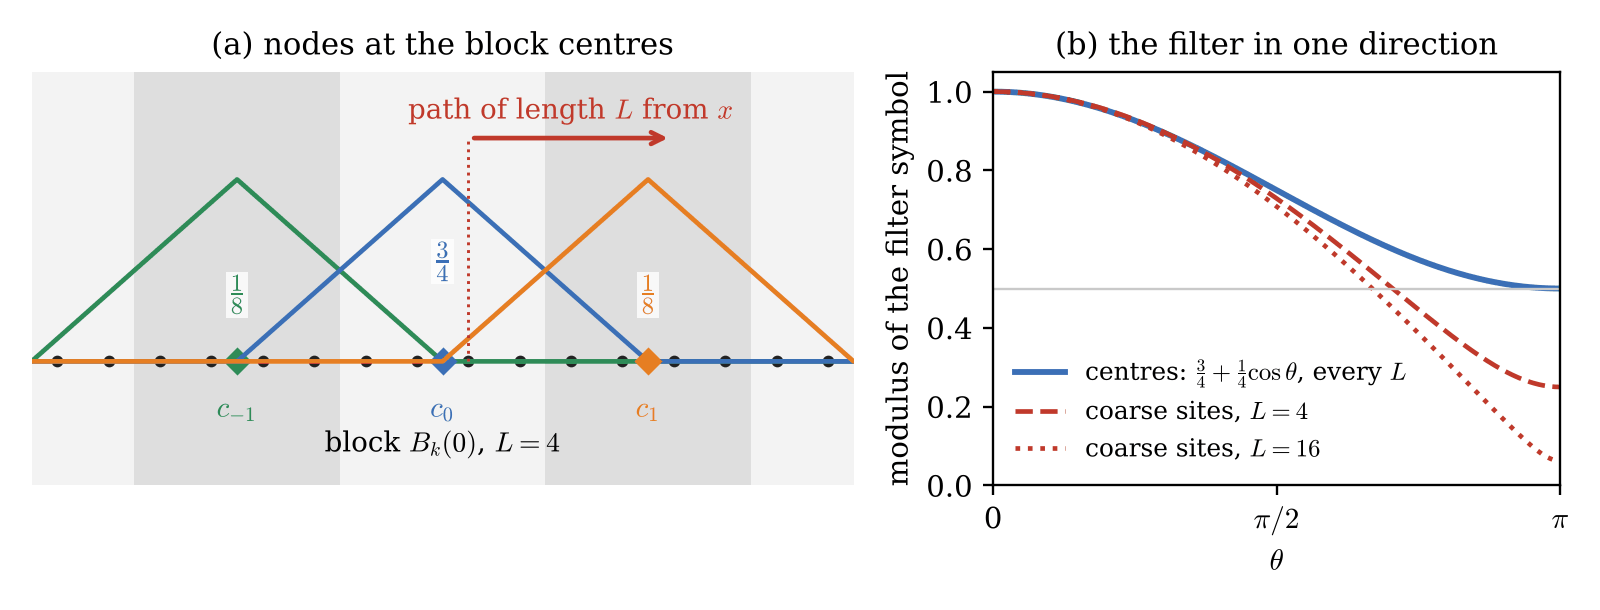
\includegraphics[width=0.95\textwidth]{figures/fig_whitney.png}
\caption{The extension of Theorem~\ref{thm:effectiveupper} along one
direction. (a)~A block of side $L=4$: the nodes are the block centres $c_z$,
the hat functions $\lambda_z$ interpolate between them, and the straight
path of length $L$ from a site $x$ meets the segments of three centres;
averaged over the block, their weights are $\frac18$, $\frac34$, $\frac18$
at every scale. (b)~The symbol of this filter stays at least $\frac12$,
while the filter obtained with the coarse sites as nodes has symbol of
modulus $1/L$ at $\theta=\pi$.}\label{fig:whitney}
\end{figure*}

\begin{lemma}\label{lem:whitney}
Let $k\ge1$, $u$ a square-summable field on the coarse links, and let $T$
act on each component of $u$ by $T=\tau_1\tau_2\tau_3\tau_4$, where
$(\tau_\nu f)(z)=\frac34f(z)+\frac18\bigl(f(z-e_\nu)+f(z+e_\nu)\bigr)$.
\begin{enumerate}[label=\textup{(\roman*)},leftmargin=*]
\item For the plaquette $p$ at $x$ in the plane $\{\mu,\nu\}$,
\[
\begin{split}
(d\Pi u)_p&=\int_0^1\!\!\int_0^1\Omega_{\mu\nu}(x+se_\mu+te_\nu)\,ds\,dt,\\
\Omega_{\mu\nu}&=\frac1{L^2}\sum_z(du)_{z,\mu\nu}\,\chi^\mu_z\chi^\nu_z
\!\!\prod_{\rho\ne\mu,\nu}\!\!\lambda^\rho_z ,
\end{split}
\]
where $(du)_{z,\mu\nu}$ is the curvature of $u$ at the coarse plaquette at
$z$ in the plane $\{\mu,\nu\}$. In particular $\Pi(db)$ is a gradient.
\item $Q(\Pi u)\le Q_k(u)$.
\item $V^{(k)}(\Pi u)=Tu$.
\end{enumerate}
\end{lemma}

\begin{proof}
(i) The function $\omega_\mu$ is continuous and piecewise linear in every
coordinate $\xi_\nu$, $\nu\ne\mu$, and $\omega_\nu$ in $\xi_\mu$. Hence
\[
\begin{split}
(d\Pi u)_p={}&\int_0^1\bigl(\omega_\mu(x+te_\mu)-\omega_\mu(x+e_\nu+te_\mu)
\bigr)dt\\
&+\int_0^1\bigl(\omega_\nu(x+e_\mu+te_\nu)-\omega_\nu(x+te_\nu)\bigr)dt
\end{split}
\]
is the integral over the unit square of $\partial_\mu\omega_\nu-\partial_\nu
\omega_\mu$, which exists almost everywhere. Since $\partial_\mu\lambda^\mu_z
=\frac1L(\chi^\mu_{z-e_\mu}-\chi^\mu_z)$ and $\chi^\nu_z$ and
$\lambda^\rho_z$, $\rho\ne\mu$, do not change when $z$ is shifted by
$e_\mu$, a shift of the summation index gives
\[
\partial_\mu\omega_\nu=\frac1{L^2}\sum_z\bigl(u_{(z+e_\mu,\nu)}-u_{(z,\nu)}
\bigr)\chi^\mu_z\chi^\nu_z\prod_{\rho\ne\mu,\nu}\lambda^\rho_z ,
\]
and the same with $\mu,\nu$ exchanged. The difference is $\Omega_{\mu\nu}$,
with $(du)_{z,\mu\nu}=u_{(z,\mu)}+u_{(z+e_\mu,\nu)}-u_{(z+e_\nu,\mu)}-
u_{(z,\nu)}$, the sign convention of the fine plaquettes. If $u=db$ then
$\Omega=0$, every curvature of $\Pi u$ vanishes, and $\Pi u$ is a gradient.

(ii) By Cauchy--Schwarz, $(d\Pi u)_p^2$ is at most the integral of
$\Omega_{\mu\nu}^2$ over the unit square of $p$. At a point $\xi$ exactly
one pair $(z_\mu,z_\nu)$ has $\chi^\mu_z\chi^\nu_z=1$, and the hat
functions form a partition of unity, $\sum_{z_\rho,z_\sigma}\lambda^\rho_z
\lambda^\sigma_z=1$ for $\{\rho,\sigma\}$ the other two directions; so
$\Omega_{\mu\nu}^2\le L^{-4}\sum_{z_\rho,z_\sigma}\lambda^\rho_z\lambda^
\sigma_z(du)^2_{z,\mu\nu}$. Summing over the plaquettes of the plane
$\{\mu,\nu\}$ integrates over $\xi_\mu,\xi_\nu$, which gives the factor
$L^2$ for each pair $(z_\mu,z_\nu)$, and sums over the integers $x_\rho,
x_\sigma$. Since $c_{z,\rho}-x_\rho$ lies in $\Z+\frac12$, $\sum_{x_\rho\in
\Z}\lambda^\rho_z=2\sum_{j=0}^{L-1}\bigl(1-\frac{j+1/2}L\bigr)=L$, and the
same for $\sigma$. So the plaquettes of the plane $\{\mu,\nu\}$ contribute
at most $L^{-4}\cdot L^2\cdot L^2\sum_z(du)^2_{z,\mu\nu}$.

(iii) By Lemma~\ref{lem:straightpaths}(i), $V^{(k)}_{y,\mu}(\Pi u)$ is the
mean over $x=Ly+s$, $s\in\{0,\dots,L-1\}^4$, of $\int_0^L\omega_\mu(x+te_\mu)
\,dt$. The term of $u_{(z,\mu)}$ in it is a product of a factor of the
coordinate $\mu$ and one of each $\nu\ne\mu$, and the mean over $s$ is the
product of the means over the single coordinates. Put $\delta=s_\mu-
\frac{L-1}2$. The interval $[x_\mu,x_\mu+L)$ meets $[c_{z,\mu},c_{z,\mu}+L)$
in length $L-|\delta|$ if $z_\mu=y_\mu$, in $\max(0,-\delta)$ if $z_\mu=
y_\mu-1$, in $\max(0,\delta)$ if $z_\mu=y_\mu+1$, and not otherwise. As $L$
is even, $\sum_s|\delta|=2\sum_{j=0}^{L/2-1}(j+\frac12)=\frac{L^2}4$, so the
means of these lengths divided by $L$ are $\frac34$, $\frac18$, $\frac18$.
For $\nu\ne\mu$ put $\delta=s_\nu-\frac{L-1}2$; then $\lambda^\nu_z(x)$ is
$1-|\delta|/L$ if $z_\nu=y_\nu$, $\max(0,\mp\delta)/L$ if $z_\nu=y_\nu\mp1$,
and zero otherwise, with the same means. The product of the four means is
the coefficient of $u_{(z,\mu)}$ in $(Tu)_{(y,\mu)}$.
\end{proof}

\begin{theorem}\label{thm:effectiveupper}
For every $k\ge1$ and every finitely supported field $w$ on the links of the
lattice of spacing $2^k$,
\[
Q_k(w)\le S_k(w)\le256\,Q_k(w).
\]
\end{theorem}

\begin{proof}
The lower bound is Proposition~\ref{prop:effective}(iii). The operator $T$
of Lemma~\ref{lem:whitney} is a convolution, the same on every component, so
it commutes with $d$; its symbol is $\prod_\nu(\frac34+\frac14\cos\theta_\nu)
\ge\frac1{16}$, so it is invertible on square-summable fields with
$\|T^{-1}\|\le16$. Let $u=T^{-1}w$. By Lemma~\ref{lem:whitney},
$V^{(k)}(\Pi u)=w$ and
\[
Q(\Pi u)\le Q_k(u)=\|T^{-1}dw\|^2\le256\,Q_k(w).
\]
It remains to replace $\Pi u$ by a finitely supported field. Let $u_R$ be
$u$ on the coarse links with base in $[-R,R]^4$ and zero elsewhere, and
$e_R=w-Tu_R=T(u-u_R)$, which is finitely supported and tends to zero.
Let $\psi_R$ equal $e_R(y,\mu)$ on the links $(x,\mu)$ with $x\in B_k(y)$
and $x_\mu\equiv L-1$ modulo $L$, and zero elsewhere. Each straight path of
length $L$ from a site of $B_k(y)$ in the direction $\mu$ contains exactly
one such link of $B_k(y)$, so $V^{(k)}(\psi_R)=e_R$ by
Lemma~\ref{lem:straightpaths}(i), and $Q(\psi_R)\le24\|\psi_R\|^2=24L^3
\|e_R\|^2$, since a link lies in six plaquettes of four links. The field
$\Pi u_R+\psi_R$ is finitely supported, its $k$-fold averages are $w$, and
$Q(\Pi u_R+\psi_R)^{1/2}\le Q_k(u_R)^{1/2}+(24L^3)^{1/2}\|e_R\|$, which
tends to $Q_k(u)^{1/2}$. Lemma~\ref{lem:straightpaths}(iii) gives
$S_k(w)\le Q_k(u)\le256\,Q_k(w)$.
\end{proof}

So at every scale the averages carry the coarse plaquette form up to a
factor at most $256$, independent of $k$. The construction inverts the
averages by a fixed convolution: the filter $(\frac18,\frac34,\frac18)$ does
not depend on the scale because the nodes are the block centres, and its
symbol is at least $\frac12$. With the coarse sites as nodes the
corresponding filter is $\frac{L+1}{2L}\delta_0+\frac{L-1}{2L}\delta_1$,
whose symbol has modulus $1/L$ at $\theta=\pi$ (Fig.~\ref{fig:whitney}(b)). In floating
point, on a grid of $12^4$ momenta, the largest ratio of $S_k$ to $Q_k$ on
curvatures is $3.9$, $7.8$ and $10.2$ for $k=1,2,3$, and the kernel of $S_k$
decreases by the factors $0.17$, $0.23$ and $0.25$ per coarse spacing; these
values are reproduced in the archive.
The theorem gives no decay. The decay comes from an exact formula for $S_k$
in Fourier variables: in a Feynman gauge for the fine field the effective
form is diagonal in the six planes, and the pole of the fine propagator at
zero momentum cancels between numerator and denominator.

For $t\in\C$ put $D_L(t)=\frac1L\sum_{j=0}^{L-1}e^{ijt}$, and for
$\vartheta\in\C^4$ put $\Psi(\vartheta)=\prod_\nu D_L(\vartheta_\nu)$,
$E_\mu(\vartheta)=e^{i\vartheta_\mu}-1$ and $\varepsilon(\vartheta)=
\sum_\nu(2-2\cos\vartheta_\nu)$. For an entire function $f$ let
$f^\sharp(\vartheta)=\overline{f(\bar\vartheta)}$, so that $ff^\sharp=|f|^2$
on real arguments. For $\theta\in\C^4$ and $n\in\{0,\dots,L-1\}^4$ let
$\theta^{(n)}=(\theta+2\pi n)/L$; every function below is $2\pi$-periodic in
each coordinate of $\theta^{(n)}$, and we take the real parts of these
coordinates in $[-\pi,\pi]$. Write $\Psi_n=(\Psi\Psi^\sharp)(\theta^{(n)})$,
$D_{n,\sigma}=(D_LD_L^\sharp)(\theta^{(n)}_\sigma)$, and put
\begin{gather*}
A_\sigma=\Psi_0D_{0,\sigma},\qquad\hat\varepsilon=L^2\varepsilon(
\theta^{(0)}),\qquad\tilde a_\sigma=A_\sigma+\hat\varepsilon r_\sigma,\\
r_\sigma=\sum_{n\ne0}\frac{\Psi_nD_{n,\sigma}}{L^2\varepsilon(\theta^{(n)})},
\end{gather*}
\begin{equation}\label{eq:Yk}
\begin{split}
Y={}&\Psi_0^3\prod_\tau D_{0,\tau}\\
&+\sum_\sigma E_\sigma E^\sharp_\sigma\sum_{\emptyset\ne J\subset\{1,2,3,4\}
\setminus\{\sigma\}}\hat\varepsilon^{|J|-1}\prod_{\tau\in J}r_\tau
\prod_{\tau\notin J\cup\{\sigma\}}A_\tau ,
\end{split}
\end{equation}
all functions of $\theta$, and for a plane $P=\{\lambda,\rho\}$
\[
K_P=\frac{\prod_{\sigma\notin P}\tilde a_\sigma}{Y}.
\]
For $L=1$ these are $\tilde a_\sigma=Y=K_P=1$. For a coarse field $w$ let
$\hat w(\theta)=\sum_ye^{-i\theta\cdot y}w_y$, and let $F_P=(dw)_P$ be its
curvature in the plane $P$, a function of the coarse sites.

\begin{lemma}\label{lem:planes}
Let $\gamma_1,\dots,\gamma_4>0$, $\Gamma=\mathrm{diag}(\gamma_\mu)$ and
$0\ne E\in\C^4$, and for $P=\{\lambda,\rho\}$, $\lambda<\rho$, let $c_P$ be
the row vector with $c_Pv=E_\lambda v_\rho-E_\rho v_\lambda$. Then
\[
\Gamma-\frac{\Gamma EE^*\Gamma}{E^*\Gamma E}
=\frac1{E^*\Gamma E}\sum_P\gamma_\lambda\gamma_\rho\,c_P^*c_P .
\]
\end{lemma}

\begin{proof}
Both sides are Hermitian. The diagonal entry $(\mu,\mu)$ of the right side
is $\sum_{\lambda\ne\mu}\gamma_\mu\gamma_\lambda|E_\lambda|^2/E^*\Gamma E$,
which is $\gamma_\mu-\gamma_\mu^2|E_\mu|^2/E^*\Gamma E$; the entry
$(\mu,\nu)$, $\mu\ne\nu$, comes only from $P=\{\mu,\nu\}$, where
$c_P$ has $-E_\nu$ in place $\mu$ and $E_\mu$ in place $\nu$, and equals
$-\gamma_\mu\gamma_\nu\bar E_\mu E_\nu/E^*\Gamma E$.
\end{proof}

\begin{theorem}\label{thm:effectivelocal}
Let $k\ge1$ and $L=2^k$.
\begin{enumerate}[label=\textup{(\roman*)},leftmargin=*]
\item The functions $K_P$ are real-analytic, even, $2\pi$-periodic and
positive on $\R^4$, $K_P(0)=1$, and for every finitely supported field $w$
on the coarse links
\[
S_k(w)=\sum_P\int_{[-\pi,\pi]^4}K_P(\theta)\,|\hat F_P(\theta)|^2\,
\frac{d\theta}{(2\pi)^4}.
\]
\item There are $\eta>0$ and $C<\infty$, independent of $k$, such that
every $K_P$ extends analytically to $\{|\mathrm{Im}\,\theta_\nu|\le\eta\}$ and
is bounded there by $C$.
\item Hence $S_k(w)=\sum_P\sum_{y,y'}\mathcal K_P(y-y')F_P(y)F_P(y')$ with
real kernels $\mathcal K_P(y)=(2\pi)^{-4}\int K_P(\theta)e^{i\theta\cdot y}\,
d\theta$ that satisfy $|\mathcal K_P(y)|\le Ce^{-\eta|y|_1}$ for every $k$.
\end{enumerate}
\end{theorem}

\begin{proof}
\emph{Step 1: the form in Fourier variables.} Let $c_\mu(q)=L\Psi(q)
D_L(q_\mu)$. Lemma~\ref{lem:straightpaths}(i) and the Poisson summation
formula give, for every square-summable field $\varphi$,
\[
\widehat{V^{(k)}(\varphi)}_\mu(\theta)=L^{-4}\sum_nc_\mu(\theta^{(n)})\,
\hat\varphi_\mu(\theta^{(n)}),
\]
with $\hat\varphi(q)=\sum_xe^{-iq\cdot x}\varphi_x$. Write $x_n=\hat\varphi(
\theta^{(n)})\in\C^4$ and $e_n=(e^{i\theta^{(n)}_\mu}-1)_\mu$, so that
$|e_n|^2=\varepsilon(\theta^{(n)})=:\varepsilon_n$. By the Lagrange identity
the plaquette form at the momentum $\theta^{(n)}$ is $\varepsilon_n|x_n|^2-
|e_n^*x_n|^2$, and the Plancherel formula gives
\[
Q(\varphi)=\int_{[-\pi,\pi]^4}L^{-4}\sum_n\bigl(\varepsilon_n|x_n|^2-
|e_n^*x_n|^2\bigr)\frac{d\theta}{(2\pi)^4}.
\]
Since $LD_L(t)(e^{it}-1)=e^{iLt}-1$ and $e^{iL\theta^{(n)}_\mu}=
e^{i\theta_\mu}$, the averages map the gauge direction at every alias to the
coarse gauge direction: $c_\mu(\theta^{(n)})(e_n)_\mu=\Psi(\theta^{(n)})
E_\mu(\theta)$. For $|t|\le\pi/L$ we have $|D_L(t)|=|\sin(Lt/2)|/
(L|\sin(t/2)|)\ge2/\pi$, so $\Psi(\theta^{(0)})\ne0$ for real $\theta$.

\emph{Step 2: the minimum at one momentum.} Fix real $\theta\notin2\pi
\Z^4$; then $E=E(\theta)\ne0$ and every $\varepsilon_n>0$. Let $z\in\C^4$.
Minimising $L^{-4}\sum_n\varepsilon_n|y_n|^2$ under $L^{-4}\sum_nc_\mu(
\theta^{(n)})(y_n)_\mu=z_\mu$ separates in $\mu$, and the Cauchy--Schwarz
inequality gives the minimum $\sum_\mu|z_\mu|^2/a_\mu$, attained at
$(y_n)_\mu=z_\mu\overline{c_\mu(\theta^{(n)})}/(\varepsilon_na_\mu)$,
where
\[
a_\mu=L^{-4}\sum_n\frac{|c_\mu(\theta^{(n)})|^2}{\varepsilon_n}
=\frac{\tilde a_\mu}{\hat\varepsilon}.
\]
If $x$ satisfies the constraint with right side $\hat w(\theta)$, write $x_n=
x_n^T+\beta_ne_n$ with $e_n^*x_n^T=0$. Then $L^{-4}\sum_n(\varepsilon_n
|x_n|^2-|e_n^*x_n|^2)=L^{-4}\sum_n\varepsilon_n|x^T_n|^2$, and by Step 1 the
vectors $x^T_n$ satisfy the constraint with right side $\hat w(\theta)+tE$
for some $t\in\C$. Hence the plaquette form at $\theta$ is at least
\[
\min_{t\in\C}\sum_\mu\frac{|\hat w_\mu+tE_\mu|^2}{a_\mu}
=\hat w^*\Bigl(\Gamma-\frac{\Gamma EE^*\Gamma}{E^*\Gamma E}\Bigr)\hat w
\]
with $\Gamma=\mathrm{diag}(a_\mu^{-1})$. Conversely, take $t$ optimal, $y$ optimal for $z=\hat w+tE$, and replace
$y_0$ by $y_0-\beta e_0$ with $\beta=L^4t/\Psi(\theta^{(0)})$: the constraint
becomes $\hat w(\theta)$ and the plaquette form does not increase, since
$e_0$ is a gauge direction. By Lemma~\ref{lem:planes} the minimum is
\[
\sum_P\frac{\gamma_\lambda\gamma_\rho}{E^*\Gamma E}|c_P\hat w|^2,\qquad
\frac{\gamma_\lambda\gamma_\rho}{E^*\Gamma E}=\frac{\prod_{\sigma\notin P}
a_\sigma}{\sum_\sigma|E_\sigma|^2\prod_{\tau\ne\sigma}a_\tau}.
\]
We multiply numerator and denominator by $\hat\varepsilon^3$ and expand
$\tilde a_\tau=A_\tau+\hat\varepsilon r_\tau$. The terms without $r$ add up
to $\Psi_0^3\prod_\tau D_{0,\tau}\sum_\sigma|E_\sigma|^2/D_{0,\sigma}$,
and $|E_\sigma|^2=L^2D_{0,\sigma}|e^{i\theta^{(0)}_\sigma}-1|^2$ by the
identity of Step 1, so they equal $\hat\varepsilon\,\Psi_0^3\prod_\tau
D_{0,\tau}$; every other term carries a factor $\hat\varepsilon$. So the
denominator is $\hat\varepsilon Y$, the numerator $\hat\varepsilon\prod_{
\sigma\notin P}\tilde a_\sigma$, and the quotient is $K_P(\theta)$. Since
$|c_P\hat w|=|\hat F_P|$, the minimum at $\theta$ is $\sum_PK_P(\theta)|\hat F_P(
\theta)|^2$.

\emph{Step 3: integration.} Integrating the lower bound over $\theta$ gives
$Q(\varphi)\ge\sum_P\int K_P|\hat F_P|^2$ for every square-summable
$\varphi$ with $V^{(k)}(\varphi)=w$. The minimisers of Step 2 are bounded by
a constant times $|\hat w(\theta)|$: for $n\ne0$ because $\varepsilon_n\ge
4/L^2$ and $a_\mu\ge A_\mu/\hat\varepsilon$; for $n=0$ because
$|c_\mu(\theta^{(0)})|/(\varepsilon_0a_\mu)\le L^3/A_\mu$; and $|t||E|\le
|\hat w|(\max\gamma/\min\gamma)^{1/2}$ by the Cauchy--Schwarz inequality for
the inner product $\Gamma$, while $|e_0|\le|\theta|/L\le\frac\pi2|E|/L$.
Here $A_\mu\ge(2/\pi)^{10}$, and $\gamma_\mu/\gamma_\nu=\tilde a_\nu/
\tilde a_\mu$ is bounded because the $\tilde a$ are continuous and at least
$A$. So the minimisers define a square-summable field $\varphi^*$ with
$V^{(k)}(\varphi^*)=w$ and $Q(\varphi^*)=\sum_P\int K_P|\hat F_P|^2$.
Since $V^{(k)}$ and $Q$ are bounded on square-summable fields, truncating
$\varphi^*$ and correcting with $\psi_R$ as in the proof of
Theorem~\ref{thm:effectiveupper} gives finitely supported fields with the
same averages and plaquette forms tending to $Q(\varphi^*)$, and
Lemma~\ref{lem:straightpaths}(iii) gives (i) for $S_k$. The functions are
even since $|D_L|^2$ and $\varepsilon$ are, and positive since $\tilde
a_\sigma\ge A_\sigma>0$ and $Y\ge\Psi_0^3\prod_\tau D_{0,\tau}\ge
(2/\pi)^{32}$ on $\R^4$, all other terms of~\eqref{eq:Yk} being non-negative
there. At $\theta=0$, $\Psi_0=D_{0,\tau}=1$ and $\hat\varepsilon=0$, so
$K_P(0)=1$.

\emph{Step 4: the strip.} Let $|\mathrm{Im}\,\theta_\nu|\le\frac12$, and for
$n$ let $s=L\theta^{(n)}$, so $|\mathrm{Re}\,s_\nu|\le\pi L$ and
$|\mathrm{Im}\,s_\nu|\le\frac12$. For $q=x+iy$ with $|x|\le\pi$,
$|e^{iq}-1|^2=(e^{-y}-1)^2+2e^{-y}(1-\cos x)\ge e^{-|y|}\frac4{\pi^2}x^2$,
so
\[
|D_L(q)|\le\min\Bigl(e^{1/2},\frac{c_1}{|\mathrm{Re}\,Lq|}\Bigr)
\]
for $|\mathrm{Im}\,q|\le1/(2L)$, where $c_1=(e^{1/2}+1)e^{1/4}\frac\pi2<5.35$, and the same holds for $D_L^\sharp$. Also
$\mathrm{Re}(2-2\cos q)\ge(2-2\cos x)-2(\cosh y-1)$, so
$\mathrm{Re}\,L^2\varepsilon(\theta^{(n)})\ge\frac4{\pi^2}|\mathrm{Re}\,
s|^2-1.2$. For $n\ne0$ some $|\mathrm{Re}\,s_\nu|\ge\pi$, and then
$|L^2\varepsilon(\theta^{(n)})|\ge0.28\,|\mathrm{Re}\,s|^2$. Writing
$s=\theta+2\pi m$ with $m\in\Z^4\setminus\{0\}$, $|\mathrm{Re}\,s_\nu|\ge
\pi|m_\nu|$, and
\[
|r_\sigma|\le\frac{c_1^{10}}{0.28\,\pi^2}\sum_{m}\prod_\nu
f(m_\nu)=\frac{c_1^{10}}{0.28\,\pi^2}\Bigl(\frac43\Bigr)^4
<2.2\cdot10^7,
\]
with $f(0)=1$ and $f(j)=1/(\pi j)^2$. The $r_\sigma$ are finite sums of
functions analytic on the strip, since no $\varepsilon(\theta^{(n)})$,
$n\ne0$, vanishes there. Further $|A_\sigma|\le e^5$, $|\hat\varepsilon|
\le4(\pi^2+\frac14)e^{1/2}<70$ and $|E_\sigma E_\sigma^\sharp|\le
(e^{1/2}+1)^2<7.1$, so on the strip $|Y|\le M=10^{28}$ and $|\tilde
a_\sigma|\le1.6\cdot10^9$, uniformly in $k$. By the Cauchy estimate on
discs of radius $\frac14$ in each variable, $|\partial_\nu Y|\le4M$ where
$|\mathrm{Im}\,\theta|\le\frac14$, so $|Y(\theta)-Y(\mathrm{Re}\,\theta)|\le
16\eta M\le\frac12(2/\pi)^{32}$ for $|\mathrm{Im}\,\theta_\nu|\le\eta=
10^{-36}$. There $|Y|\ge\frac12(2/\pi)^{32}$, $K_P=\prod_{\sigma\notin P}
\tilde a_\sigma/Y$ is analytic, and $|K_P|\le C=10^{26}$, which is (ii).
Moving the contour of each $\theta_\nu$ to $\mathrm{Im}\,\theta_\nu=
\pm\eta$, according to the sign of $y_\nu$, gives (iii); the kernels are
real because $K_P$ is real and even.
\end{proof}

The proof makes $\eta$ explicit but very small. In floating point the
kernels decrease much faster: $\max|\mathcal K_P(y)|$ over $|y|_1=d$ falls
by factors $0.17$, $0.24$ and $0.26$ per unit of $d$ for $k=1,2,3$, the largest value of
$K_P$ on $\R^4$ is $4.4$, $8.7$ and $11.3$, and its smallest value is $1$, attained at
$\theta=0$ (Fig.~\ref{fig:locality}); these computations are reproduced in
the archive. Each $K_P$ is a Riemann sum in $n$ of a function of
$\theta+2\pi n$, so the kernels have a limit as $k\to\infty$; the theorem
does not use it. Uniform decay of the propagators of the averaging
operations of lattice gauge theories is the subject of Ba{\l}aban's
work~\cite{Bal84a}; here the hard constraint and the Feynman gauge make the
effective form itself explicit. Together with Theorem~\ref{thm:effectiveupper},
the effective forms of the quadratic approximation are equivalent to the
coarse plaquette forms and local, with constants independent of the scale.

\begin{figure*}[t]
\centering
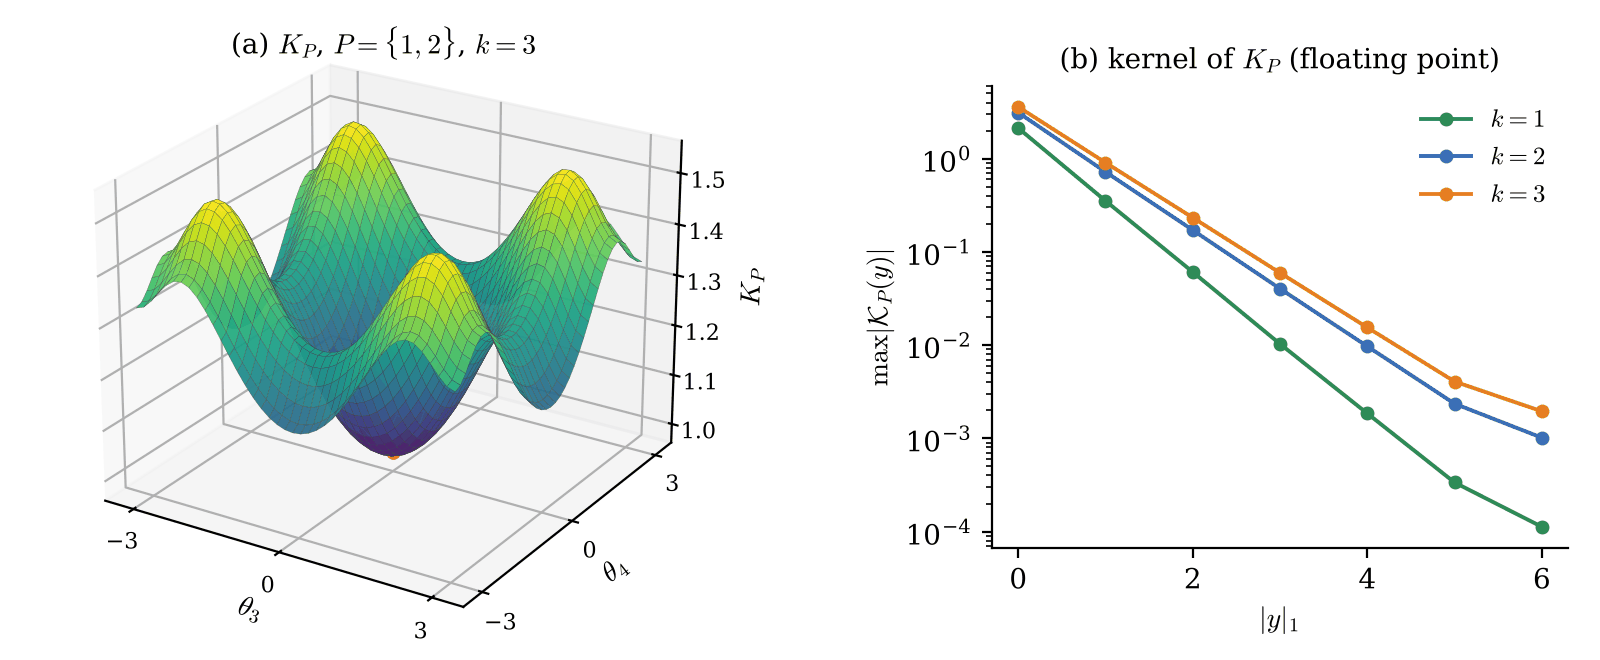
\includegraphics[width=0.95\textwidth]{figures/fig_locality.png}
\caption{The effective forms of Theorem~\ref{thm:effectivelocal}.
(a)~The multiplier $K_P$ for the plane $P=\{1,2\}$ at $k=3$, as a function of
$(\theta_3,\theta_4)$ with $\theta_1=\theta_2=0$; it equals $1$ at $\theta=0$
and stays bounded. (b)~The largest value of the kernel $|\mathcal K_P(y)|$
on $|y|_1=d$ for $k=1,2,3$, in logarithmic scale: the decay per coarse
spacing hardly changes with $k$.}\label{fig:locality}
\end{figure*}

\begin{lemma}\label{lem:mixture}
Let $(X,d_X)$ and $(Y,d_Y)$ be Polish spaces, $\rho,\rho'$ Borel probability
measures on $Y$, and $\kappa,\kappa'$ probability kernels from $Y$ to $X$,
all with finite first moments. If $W_1(\kappa(\cdot\mid v),\kappa'(\cdot\mid
v))\le\varepsilon$ and $W_1(\kappa'(\cdot\mid v),\kappa'(\cdot\mid v'))\le
d_Y(v,v')$ for all $v,v'$, then the mixtures $\pi=\int\kappa(\cdot\mid v)\,
\rho(dv)$ and $\pi'=\int\kappa'(\cdot\mid v)\,\rho'(dv)$ satisfy
\[
W_1(\pi,\pi')\le\varepsilon+W_1^{d_Y}(\rho,\rho').
\]
\end{lemma}

\begin{proof}
Let $F$ be $1$-Lipschitz on $X$ and $\kappa F(v)=\int F\,d\kappa(\cdot\mid
v)$. Then $\int F\,d\pi-\int F\,d\pi'=\int(\kappa F-\kappa'F)\,d\rho+\bigl(
\int\kappa'F\,d\rho-\int\kappa'F\,d\rho'\bigr)$. The first term is at most
$\varepsilon$. The function $\kappa'F$ is $1$-Lipschitz for $d_Y$, so the
second is at most $W_1^{d_Y}(\rho,\rho')$. The Kantorovich--Rubinstein
duality gives the claim.
\end{proof}

A law $\gamma$ on $\R^V$ \emph{decomposes along the averages} if
$\gamma(\cdot\mid\eta)=\int\gamma^{\rm c}_V(\cdot\mid\eta,v)\,\rho_V(dv\mid
\eta)$, with $\rho_V(\cdot\mid\eta)$ the law of $(V_{y,\mu})_{y\in W}$. Every
law with density proportional to $\exp(-\frac b2\sum_{p\cap V\ne\emptyset}
(d\varphi)_p^2)\,g(V(\varphi))$, on a set cut out by conditions on the
averages, decomposes in this way, because Lebesgue measure disintegrates
along the fibres of a surjective linear map into multiples of Lebesgue
measure on the fibres. Here $g$ can carry any action of the averages, in
particular a coarse gauge fixing and a coarse effective action, which is
the form a law takes after the fine scale has been integrated out.

\begin{corollary}\label{cor:compose}
Let $r_w\in\R^V$ minimise $\sum_{p\cap V\ne\emptyset}(d\varphi)_p^2$, with
zero exterior, subject to $V_{y',\mu'}(r_w)=\delta_{w,(y',\mu')}$ for all
$(y',\mu')$, $y'\in W$; put $L_w=\|r_w\|_1$ and $d_L(v,v')=\sum_wL_w
|v_w-v'_w|$. For every law that decomposes along the averages,
\[
C_{V,j}\le C^{\rm c}_{V,j}+C^\rho_{V,j},\qquad C^\rho_{V,j}=\sup\frac{W_1^{
d_L}(\rho_V(\cdot\mid\eta),\rho_V(\cdot\mid\eta'))}{|\eta_j-\eta'_j|},
\]
the supremum over exteriors that differ only at $j$, and $L_w\le4\cdot
10^{14}$. Hence $K_c\le K^{\rm c}_c+K^\rho_c$ with $K^\rho_c=\sum_{j\in
c\setminus V}C^\rho_{V,j}$, and if $K^\rho_c\le\frac\alpha2N_n$ for every
class and $n\ge4\cdot10^{15}/\alpha$, then $D(n,\alpha)$ holds for the law, with the $49$ classes of active links.
\end{corollary}

\begin{proof}
Apply Lemma~\ref{lem:mixture} with $\kappa=\gamma^{\rm c}_V(\cdot\mid\eta,
\cdot)$, $\kappa'=\gamma^{\rm c}_V(\cdot\mid\eta',\cdot)$, $\rho=\rho_V(\cdot
\mid\eta)$, $\rho'=\rho_V(\cdot\mid\eta')$. The first condition holds with
$\varepsilon=C^{\rm c}_{V,j}|\eta_j-\eta'_j|$. By
Theorem~\ref{thm:constrainedcube}(i) the laws $\gamma^{\rm c}_V(\cdot\mid
\eta',v)$ and $\gamma^{\rm c}_V(\cdot\mid\eta',v')$ are translates by
$\sum_w(v'_w-v_w)r_w$, so their distance is at most $d_L(v,v')$. For the
bound on $L_w$, the pair $(r_w,y)$ solves $K(r_w,y)=(0,s\,e_w)$ with $K$ as
in the proof of Theorem~\ref{thm:constrainedcube}. Measure $d$ from the
centre of the row $w$; Lemma~\ref{lem:combes} gives $\sum_ee^{2\lambda d(e)}
r_w(e)^2\le(2M_0s)^2=20160^2$. With $z_0=2y+e_\mu$ for $w=(y,\mu)$, a link
whose base is at distance $k$ from $z_0$ has its midpoint at distance at
least $k-1$ from the centre, and the count in that proof gives $L_w^2\le
20160^2\cdot4e^{2\lambda}\bigl(1+\sum_{k\ge1}(64k^3+16k)e^{-2\lambda k}\bigr)
\le(4\cdot10^{14})^2$. Summing over the translates as in
Definition~\ref{def:cube} gives $K_c\le K^{\rm c}_c+K^\rho_c$, and
Theorem~\ref{thm:constrainedcube}(iii) with $\alpha/2$ in place of $\alpha$
gives $K^{\rm c}_c\le\frac\alpha2N_n$.
\end{proof}

The responses are much smaller than the bound: in floating point,
$\max_wL_w$ is $23.8$, $44.1$ and $50.9$ for the block $(m,m,m,m)$,
$m=\lfloor n/4\rfloor$, of the cubes $n=4$, $6$, $8$. Since
Theorem~\ref{thm:constrainedcube} controls the first term at every coupling,
the corollary reduces $D(n,\alpha)$ for a law that decomposes along the
averages to the cube condition $K^\rho_c$ for its averages, a problem of the
same form one scale up, in the metric $d_L$. Iterating it needs
Theorem~\ref{thm:constrainedcube} and the corollary with $S_k$ in place of
the plaquette form, which Theorem~\ref{thm:constrainedscales} below gives
with constants independent of $k$, and ends in
a cube condition for the coarsest averages, which is where a gap has to come
from: the quadratic approximation describes a massless field and has none.
The corollary is one step of the composition of
Remark~\ref{rem:constrainedopen}(a), not its conclusion.

On the lattice of spacing $2^k$ the blocks, the tree links, the active links
and the averages are those of Definition~\ref{def:blockgauge}, and after $k$
steps the averages of the quadratic approximation carry the form $S_k$. Let
$(S_{ab})$ be its matrix, $S_k(w)=\sum_{a,b}S_{ab}w_aw_b$ for finitely
supported $w$, and $d(a,b)$ the $\ell^\infty$ distance between the midpoints
of the links $a$ and $b$. Each link lies in six plaquettes of four links, and
the midpoints of the links of the plaquettes at $y$ and $y'$ are at distance
at most $|y-y'|_1+1$, so Theorem~\ref{thm:effectivelocal}(iii) gives, for
every non-decreasing $\phi\ge0$,
\begin{equation}\label{eq:Srows}
\sum_b|S_{ab}|\,\phi(d(a,b))\le24C\sum_{z\in\Z^4}e^{-\eta|z|_1}\phi(|z|_1+1),
\end{equation}
with $C$ and $\eta$ of that theorem. In particular $\sum_bS_{ab}\eta_b$
converges for every bounded field $\eta$. For $n$, $V$, $W$ as before, a
bounded exterior $\eta$ and values $v$, let $\gamma^{{\rm c},k}_V(\cdot\mid
\eta,v)$ be the law on $\R^V$ with density proportional to
\[
\exp\Bigl(-\frac b2\Bigl(\sum_{a,b\in V}S_{ab}w_aw_b+2\sum_{a\in V,\,b\notin
V}S_{ab}w_a\eta_b\Bigr)\Bigr)
\]
on the affine set $\{V_{y,\mu}(w)=v_{y,\mu},\ y\in W\}$, the conditional law
of the Gaussian with the form $bS_k$ given the exterior and the averages.
Define $C^{{\rm c},k}_{V,j}$, $K^{{\rm c},k}_c$, $D^k_{\rm c}(n,\alpha)$,
$r^{(k)}_w$ and $L^{(k)}_w$ as in Theorem~\ref{thm:constrainedcube} and
Corollary~\ref{cor:compose}, with $S_k$ in place of the plaquette form; for
$k=0$ they are the former ones.

\begin{lemma}\label{lem:combeslong}
Let $K$ be an invertible symmetric matrix indexed by a finite set $X$, with
$\|K^{-1}\|\le M_0$, and let $d:X\to\R$ and $\lambda>0$. If $\sum_b|K_{ab}|
(e^{\lambda|d(a)-d(b)|}-1)\le\frac1{2M_0}$ for every $a$, then $\|e^{\lambda
d}K^{-1}e^{-\lambda d}\|\le2M_0$.
\end{lemma}

\begin{proof}
$e^{\lambda d}Ke^{-\lambda d}=K+E$ with $|E_{ab}|\le|K_{ab}|(e^{\lambda|d(a)-
d(b)|}-1)$, a symmetric bound, so $\|E\|\le\frac1{2M_0}$ by the Schur test,
and the proof of Lemma~\ref{lem:combes} applies.
\end{proof}

\begin{theorem}\label{thm:constrainedscales}
Let $\lambda_1=10^{-215}$. For every $k\ge1$, every $b>0$, every even $n$
and every exterior link $j$:
\begin{enumerate}[label=\textup{(\roman*)},leftmargin=*]
\item $\gamma^{{\rm c},k}_V(\cdot\mid\eta,v)$ is a Gaussian law whose
covariance depends on neither $\eta$ nor $v$ and whose mean is affine in
$(\eta,v)$, and $C^{{\rm c},k}_{V,j}=\|u_j\|_1$, where $u_j\in\R^V$
minimises $S_k(u+\delta_j)$ subject to $Bu=g$, with $B$ and $g$ as in
Theorem~\ref{thm:constrainedcube};
\item $\sum_{e\in V}e^{2\lambda_1d(e)}u_j(e)^2\le10^{350}$ and $\|u_j\|_1\le
10^{607}e^{-\lambda_1r_j/2}$, where $d(e)=d(e,j)$ and $r_j=\min_{e\in V}d(e)$;
and $L^{(k)}_w\le10^{438}$ for every $w$;
\item $D^k_{\rm c}(n,\alpha)$ holds for every $\alpha\in(0,1)$ and every even
$n\ge10^{827}/\alpha$;
\item Corollary~\ref{cor:compose} holds on the lattice of spacing $2^k$,
with $S_k$ in place of the plaquette form, $L^{(k)}_w\le10^{438}$ and
$n\ge2\cdot10^{827}/\alpha$.
\end{enumerate}
None of these constants depends on $k$ or on $b$.
\end{theorem}

\begin{proof}
(i) Let $H=(S_{ab})_{a,b\in V}$. A vector $w\in\ker B$, extended by zero, lies
in the space $\Phi_W$ of the lattice of spacing $2^k$, so
Proposition~\ref{prop:effective}(iv) gives $\langle w,Hw\rangle=S_k(w)\ge
\frac1{52}|w|^2$ on $\ker B$. The proof of
Theorem~\ref{thm:constrainedcube}(i) applies, the exterior entering through
the linear term $\sum_{b\notin V}S_{ab}\eta_b$; changing $\eta_j$ by one
translates the mean by the minimiser of $\langle u,Hu\rangle+2\sum_{a\in V}
u_aS_{aj}=S_k(u+\delta_j)-S_k(\delta_j)$ subject to $Bu=g$.

(ii) The pair $(u_j,y)$ solves $K(u_j,y)=(f,sg)$ with $K$ built from $H$ and
$B$ as in Lemma~\ref{lem:saddle} and $f=-(S_{aj})_{a\in V}$. Since $Q_k(w)\le
24|w|^2$, Theorem~\ref{thm:effectiveupper} gives $\|H\|\le h=6144$; take
$s=4h=24576$. The bounds of Lemma~\ref{lem:saddle} for $(h,s)$ are at most
those for $(24,96)$, because $|x_1|$ and $|f|/s$ decrease while $h|x_1|$ and
$h/s$ do not change, so $\|K^{-1}\|\le M_0=105$ as in the proof of
Theorem~\ref{thm:constrainedcube}. Index the rows of $B$ by centres as there.
For $\phi(r)=e^{\lambda r}-1\le\lambda re^{\lambda r}$ and $\lambda\le\eta/2$,
\eqref{eq:Srows} bounds the row sums of Lemma~\ref{lem:combeslong} over $H$ by
\begin{multline*}
24C\lambda e^\lambda\sum_z(|z|_1+1)e^{-\eta|z|_1/2}\\
\le24C\lambda e^\lambda\Bigl(1+16\cdot24\,e^{\eta/2}\Bigl(\frac2\eta
\Bigr)^5\Bigr),
\end{multline*}
since at most $8r^3$ points have $|z|_1=r\ge1$ and $\sum_{r\ge1}r^pe^{-xr}\le
e^xp!/x^{p+1}$. The entries of $sB^\top$ add at most $\frac s8(e^\lambda-1)$
and a row of $sB$ gives $2s(e^\lambda-1)$. At $\lambda=\lambda_1$ the sums
are below $3\cdot10^{-4}<\frac1{2M_0}$, so
Lemma~\ref{lem:combeslong} gives $\|e^{\lambda_1d}K^{-1}e^{-\lambda_1d}\|\le
210$. By~\eqref{eq:Srows}, $\|e^{\lambda_1d}f\|\le24Ce^{\lambda_1}\sum_z
e^{-(\eta-\lambda_1)|z|_1}=24Ce^{\lambda_1}\coth^4\frac{\eta-\lambda_1}2<
4\cdot10^{172}$, and $\|e^{\lambda_1d}sg\|\le e^{\lambda_1}s/16$, which gives the
first bound. The links with base at $\ell^\infty$ distance $m$ from the base
of $j$ number at most $4(64m^3+16m)$, with midpoints at distance at least
$m-1$, so
\[
Z(x)=\sum_ee^{-xd(e)}\le4e^x\Bigl(1+\frac{384e^x}{x^4}+\frac{16e^x}{x^2}
\Bigr),
\]
and $Z(\lambda_1)<10^{864}$.
As $d\ge r_j$ on $V$, the Cauchy--Schwarz inequality gives $\|u_j\|_1^2\le
10^{350}e^{-\lambda_1r_j}Z(\lambda_1)$. Finally $(r^{(k)}_w,y)$ solves
$K(r^{(k)}_w,y)=(0,se_w)$; measuring $d$ from the centre of the row $w$,
we get $\sum_ee^{2\lambda_1d(e)}r^{(k)}_w(e)^2\le(210s)^2$ and $L^{(k)}_w\le210s\,
Z(2\lambda_1)^{1/2}<10^{438}$.

(iii) The exterior links of a class have their bases at $\ell^\infty$ distance
$m\ge1$ from $[0,n-1]^4$; at most $4((n+2m)^4-(n+2m-2)^4)\le128(n^3+8m^3)$
of them have distance $m$, and for them $r_j\ge m-1$. With
$q=\lambda_1/2$, (ii) gives
\[
K^{{\rm c},k}_c\le10^{607}\cdot128\,e^{2q}\Bigl(\frac{n^3}q+\frac{48}{q^4}
\Bigr),
\]
which is at most $\alpha N_n=\alpha(n/2)^4$ when $n\ge10^{827}/\alpha$.

(iv) The proof of Corollary~\ref{cor:compose} uses the plaquette form only
through Theorem~\ref{thm:constrainedcube}, the translation property of (i)
and the bound on $L_w$, which (i)--(iii) provide.
\end{proof}

The constants are poor because the strip of Theorem~\ref{thm:effectivelocal}
has width $10^{-36}$; they are checked in exact arithmetic in the archive.
What the theorem adds is that none of them depends on the scale: the
constrained cube condition holds with one cube side at every scale, and the
weights $L^{(k)}_w$ of the metrics $d_L$ are bounded uniformly. It does not
compose the scales. The cube condition $K^\rho_c$ that
Corollary~\ref{cor:compose} leaves at scale $k$ concerns the law of the
averages given the fine exterior, in the metric $d_L$, and it has to be turned
into the cube condition of the law one scale up; that step and the cube
condition for the coarsest averages are open, and in the quadratic
approximation the coarsest averages carry a massless Gaussian, so a gap has
to come from beyond it.

\begin{remark}\label{rem:constrainedopen}
Theorem~\ref{thm:constrainedcube} is the weak-coupling half of the
constrained route at leading order, and Theorem~\ref{thm:transfer} cannot
use it as it stands. Four steps remain, each an open problem.
\begin{enumerate}[label=\textup{(\alph*)},leftmargin=*]
\item \emph{Composition.} $D_{\rm c}$ holds the block averages fixed. A gap
in physical units needs a theorem that combines the constrained conditions
at all scales with a cube condition for the coarsest averages, in the place
of Theorem~\ref{thm:transfer}. Corollary~\ref{cor:compose} is one step of
it, Proposition~\ref{prop:effective}(iv) gives the gap at every scale, and
Theorem~\ref{thm:effectiveupper} the equivalence of $S_k$ and $Q_k$
uniformly in $k$, Theorem~\ref{thm:effectivelocal} the locality of $S_k$
uniformly in $k$, and Theorem~\ref{thm:constrainedscales} the constrained
cube condition and the bounds on the weights $L_w$ at every scale with
constants independent of $k$. Turning the cube condition for the averages
into that of the law one scale up, and a cube condition for the coarsest
averages, are open.
\item \emph{Beyond the quadratic approximation.} For the Wilson measure the
block averages are products of group elements along paths, their level sets
are curved, and the Bakry--\'Emery tensor of Sec.~\ref{sec:curvature} is
negative at large fields; Theorem~\ref{thm:blockgap} controls only the small
fields, and the large fields have to be split off as in Ba{\l}aban's
analysis~\cite{Bal89b}. For the straight paths between block roots the
group-valued estimate holds for all fields (Theorem~\ref{thm:pathcoercive}),
but that map does not compose across scales
(Proposition~\ref{prop:thinpath}), and for every compact connected group no continuous covariant
map treats the transverse positions of a block alike
(Proposition~\ref{prop:nomean}). The cut-off average of
Theorem~\ref{thm:cutoff} is coercive for all fields and agrees with the
averages to first order, with constants for one step; on torus-valued
fields of small curvature it composes (Theorem~\ref{thm:torusscales}), and
for every compact group it composes on fields whose curvature is small at
every scale with a small sum (Theorem~\ref{thm:smallscales}); under the Wilson measure
the remaining large fields form microscopic clusters
(Corollary~\ref{cor:defectclusters}), but the conditional estimate needed
near them is open. Away from them, on the fibres of the cut-off average,
the Hessian of the action along the fibre is at least $\lambda(\frac1{26}-
c_G\kappa)$ at every background with plaquettes at most $\kappa$
(Theorem~\ref{thm:smallfibre}), and on a convex chart of the fibre the
constrained law satisfies a Brascamp--Lieb inequality for large $\lambda$
(Theorem~\ref{thm:fibrechart}), and on a product chart its covariances
decay exponentially (Theorem~\ref{thm:chartdecay}); the remaining
small-field steps are listed in Remark~\ref{rem:chartdecayopen}.
\item \emph{Second order.} Let $b_0=11N/(48\pi^2)$ for $\SU(N)$, $t=2b_0\log2$,
and let $g_m^{-2}=g_*^{-2}+tm$ be the one-loop coupling $m$ steps above a
matching scale. Comparison with integrals gives $\sum_{m\le M}g_m^2=
t^{-1}\log M+O(1)$ and $\sum_mg_m^4\le\pi^2/(6t^2)$~\cite{Loc26}. A loss $1+cg_m^2$ per step therefore
compounds to a power of $M$, and a step from one scale to the next has to be
exact at order $g^2$, with that term absorbed into the running coupling and
the normalisation of the field, and remainders of order $g^4$.
\item \emph{Crossover and existence.} The passage from weak coupling to the
strong-coupling range of Sec.~\ref{sec:su2}--\ref{sec:su3blocks} and the
existence of the limit, (E), are untouched.
\end{enumerate}
The renormalisation group needed for (a) and (b) is the ultraviolet half of
(E), so the constrained route places both residues on one construction.
\end{remark}

\subsection{Path blocks for the group-valued links}\label{ssec:pathblocks}

Remark~\ref{rem:constrainedopen}(b) asks for estimates on the actual
group-valued links. They can be proved for a coarser block map, the
straight path between block roots, and this map exhibits the second half of
the difficulty: it does not compose across scales. A topological argument
shows why no continuous map that treats the transverse positions alike can
take its place.

Let $G\subset\U(r)$ be a compact matrix group, $\delta(A,B)=\lVert A-B
\rVert_{\rm HS}$, which is invariant under left and right multiplication,
and work on the periodic lattice of side $2L$ with the block tree of
Definition~\ref{def:blockgauge}, all fifteen tree links of each block equal
to $I$. Write $\mathcal B$ for the number of blocks. The \emph{path map} is
\[
V^{\rm p}_{y,\mu}(U)=U_{2y+e_\mu,\mu},
\]
the product along the straight path from $2y$ to $2y+2e_\mu$, whose first
link is a tree link; it transforms as a link under the gauge
transformations at the block roots. Fixing $V^{\rm p}=v$ fixes four of the
$49$ active links of each block, so the fibre is $G^{45\mathcal B}$, and
the Wilson law in the tree gauge restricts to it with product Haar measure
as reference, since the tree gauge has unit Jacobian. The
\emph{reconstruction} $R(v)$ puts $R_{2y+o,\mu}=v_{y,\mu}$ if $o_\mu=1$ and
$R_{2y+o,\mu}=I$ otherwise. For $U$ in the fibre of $v$ put
\[
D_v(U)^2=\sum_e\delta(U_e,R_e(v))^2,\qquad Q(U)=\sum_p\delta(U_p,I)^2,
\]
the first sum having zero terms on the tree and path links, and let
$Q_1(v)=\sum_P\delta(v_P,I)^2$ on the coarse lattice.

\begin{lemma}\label{lem:anchorcube}
For vectors $z_a$ of a real Hilbert space indexed by $a\in\{0,1\}^3$, with
$z_0=0$,
\[
\sum_a\lVert z_a\rVert^2\le\frac{3+\sqrt7}2\sum_{\{a,a'\}}\lVert z_a-
z_{a'}\rVert^2\le3\sum_{\{a,a'\}}\lVert z_a-z_{a'}\rVert^2,
\]
the sums on the right over the twelve edges of the cube.
\end{lemma}

\begin{proof}
It suffices to treat real numbers. The right side is $\ip z{L_0z}$, where
$L_0$ is the Laplacian of the cube with the vertex $0$ deleted, and the
claim is that its least eigenvalue is $3-\sqrt7$. The permutations of the
coordinates commute with $L_0$. On the functions $f_k$ of the level $k=
|a|$, $L_0$ acts by $f_1\mapsto3f_1-2f_2$, $f_2\mapsto3f_2-2f_1-f_3$,
$f_3\mapsto3f_3-3f_2$, whose characteristic polynomial in $t=3-\lambda$ is
$t^3-7t$; the eigenvalues are $3$ and $3\pm\sqrt7$. On the functions of
levels one and two whose sum over each level vanishes, indexed by the
coordinate that is one at level one and zero at level two, $L_0$ acts by
the matrix $\bigl(\begin{smallmatrix}3&1\\1&3\end{smallmatrix}\bigr)$, with
eigenvalues $2$ and $4$; at level three these functions vanish. The two
spaces have dimensions $3$ and $4$ and span $\R^7$. Finally $1/(3-\sqrt7)=
(3+\sqrt7)/2<3$.\footnote{The constant $(3+\sqrt7)/2$ is attained by a
function of the level $|a|$ alone, so it is the best constant in the
lemma.}
\end{proof}

\begin{theorem}\label{thm:pathcoercive}
For every $G\subset\U(r)$, every $L\ge1$, every $v$ and every $U$ in the
fibre of $v$,
\[
D_v(U)^2\le224\,Q(U).
\]
\end{theorem}

\begin{proof}
Let $I_0$ be the sum of $\delta(U_e,I)^2$ over the active links inside the
blocks and $J_0$ the sum of $\delta(U_e,v_{y,\mu})^2$ over the links that
leave $B(y)$ in the direction $\mu$, so $D_v^2=I_0+J_0$. For an active link
inside a block, the chain of plaquettes in the proof of
Theorem~\ref{thm:blockgap} applies to group elements: each plaquette of the
chain has its two transverse links on the tree, so the holonomy is the
product of two consecutive links of the chain, and invariance of $\delta$
with the triangle inequality gives $\delta(U_e,I)^2\le k\sum_i\delta(U_{p_i}
,I)^2$ with $k\le3$. The loads are those of that proof, so $I_0\le8Q_{\rm
in}$. Fix $y,\mu$ and label the eight links leaving $B(y)$ by the
transverse offset $a\in\{0,1\}^3$; the link $a=0$ is the path link and
equals $v_{y,\mu}$. For a transverse edge $\{a,a'\}$ the face plaquette
has holonomy $U_a\psi'U_{a'}^{-1}\psi^{-1}$ with $\psi,\psi'$ links inside
the two blocks, so $\delta(U_a,U_{a'})\le\delta(U_p,I)+\delta(\psi,I)+
\delta(\psi',I)$. Lemma~\ref{lem:anchorcube} with $z_a=U_a-v_{y,\mu}$ in
the real Hilbert--Schmidt space and Cauchy--Schwarz bound the eight terms by
$9$ times the sum of the three squares over the twelve edges. Each face
plaquette occurs once, and each link inside a block occurs once for each of
the three directions other than its own, as in the proof of
Theorem~\ref{thm:blockgap}. Hence $J_0\le9Q_{\rm face}+27I_0$ and
$D_v^2\le28I_0+9Q_{\rm face}\le224\,Q$.
\end{proof}

The bound holds for all fields, with no small-field condition and no
logarithmic chart; Theorem~\ref{thm:blockgap} is its linearisation for the
averages, with the better constant $52$.

\begin{proposition}\label{prop:pathenergy}
$Q_1(V^{\rm p}(U))\le4Q(U)$, $Q(R(v))=4Q_1(v)$ and $Q(U)\le8Q_1(v)+
48D_v(U)^2$ for $U$ in the fibre of $v$; if $Q_1(v)=0$, then $Q(U)\le
24D_v(U)^2$.
\end{proposition}

\begin{proof}
The holonomy of a coarse plaquette is that of the square of side two at
$2y$, a product of four conjugated fine plaquette holonomies, so
$\delta(v_P,I)\le\sum_{p\subset P}\delta(U_p,I)$; these squares tile each
coordinate plane, which gives the first bound. In $R(v)$ only the
plaquettes with offset one in both directions carry holonomy, equal to that
of the coarse plaquette, four for each $P$. For any plaquette,
telescoping gives $\delta(U_p,R_p)\le\sum_{e\in p}\delta(U_e,R_e)$, so
$\delta(U_p,I)^2\le2\delta(R_p,I)^2+8\sum_{e\in p}\delta(U_e,R_e)^2$, and
each link lies in six plaquettes. If $Q_1(v)=0$, every $R_p$ is $I$ and the
factor $2$ is not needed.
\end{proof}

Let $m=45\mathcal B$, let the action be $\lambda Q$ with $\lambda\ge0$
(for $\SU(N)$, $\lambda=\beta/(2N)$ up to a constant), and put
\[
z_G(t)=\int_Ge^{-t\delta(g,I)^2}dg,\qquad Z_\lambda(v)=\int_{G^m}
e^{-\lambda Q(U)}dU,
\]
with normalised Haar measures, the integral over the fibre of $v$.

\begin{theorem}\label{thm:pathZ}
For every $v$,
\[
e^{-8\lambda Q_1(v)}z_G(48\lambda)^m\le Z_\lambda(v)\le e^{-\lambda
Q_1(v)/8}z_G(\lambda/448)^m,
\]
and if $Q_1(v)=0$, then $z_G(24\lambda)^m\le Z_\lambda(v)\le z_G(\lambda/
224)^m$. Let $A_\lambda=z_G(\lambda/448)/z_G(24\lambda)$. Under the
conditional law at such a $v$,
\[
\E\,e^{\lambda D_v^2/448}\le A_\lambda^m,\qquad \E\,\delta(U_e,I)^2\le
\frac{20160}\lambda\log A_\lambda
\]
for each link $e$ when $v\equiv I$, and $A_\lambda\to10752^{q/2}$ as
$\lambda\to\infty$ if $G$ has dimension $q\ge1$.
\end{theorem}

\begin{proof}
By Theorem~\ref{thm:pathcoercive} and Proposition~\ref{prop:pathenergy},
$Q\ge\frac12(D_v^2/224+Q_1/4)$ and $Q\le8Q_1+48D_v^2$. Each term of
$D_v^2$ involves one free link, and right multiplication by $R_e(v)^{-1}$
preserves Haar measure, so $\int e^{-tD_v^2}dU=z_G(t)^m$; this gives the
two bounds, and the flat case is the same with $Q\le24D_v^2$. Next,
$-\lambda Q+\lambda D_v^2/448\le-\lambda D_v^2/448$, and integration with
the lower bound gives the exponential moment; Jensen's inequality gives
$\E D_v^2\le(448m/\lambda)\log A_\lambda$. When $v\equiv I$ the law is
invariant under translation by blocks, so the $\mathcal B$ links of each
of the $45$ classes have equal expectations, and $448\cdot45=20160$.
Finally, in exponential coordinates $\delta(e^X,I)^2=\lVert X\rVert^2+
O(\lVert X\rVert^4)$ and the Haar density is smooth and positive at $0$,
while $\delta(\cdot,I)$ is bounded below away from $I$; so $z_G(t)\sim c_G
t^{-q/2}$, and the ratio at $\lambda/448$ and $24\lambda$ tends to
$(24\cdot448)^{q/2}$.
\end{proof}

So the fluctuations of the free links around a flat path field are of
order $\lambda^{-1/2}$ uniformly in the volume, for the group variables
themselves. The path map cannot be iterated, however, and this is where it
differs from the averages. Write $V^{{\rm p},k}$ for the $k$-fold path map,
the straight path of length $s=2^k$, and $Q_k$ for the plaquette energy of
the lattice of spacing $s$.

\begin{proposition}\label{prop:thinpath}
On the periodic lattice of side $3s$, $s=2^k$, there are $\SU(2)$ fields in
the tree gauge with
\[
\frac{Q(U)}{Q_k(V^{{\rm p},k}(U))}=s\sin^2\frac\pi{2s}\le\frac{\pi^2}{4s}.
\]
For the averages, by contrast, $Q_k(V^{(k)}(\varphi))\le Q(\varphi)$ for
every $k$ in the quadratic approximation
(Proposition~\ref{prop:effective}(i)).
\end{proposition}

\begin{proof}
Let $T=\operatorname{diag}(i\pi/2,-i\pi/2)$. Put the $s/2$ links in the
direction $0$ at $(j,0,0,0)$, $j$ odd, $j<s$, equal to $e^{2T/s}$ and all
other links equal to $I$. These links have offset one in the direction $0$,
so the tree gauge holds, and the links at even $j$ are tree links. The
path from $0$ to $se_0$ carries $e^T$ and every other path carries $I$, so
one coarse link is $e^T$, and it lies in six coarse plaquettes, each with
$\delta^2=\lVert e^T-I\rVert_{\rm HS}^2=4$: $Q_k=24$. No fine plaquette
contains two of the changed links, since the two links of a plaquette in
the direction $0$ differ in a transverse coordinate, so there are $3s$
nonzero fine plaquettes, each with $\delta^2=8\sin^2(\pi/2s)$, and
$Q=24s\sin^2(\pi/2s)$. Gauge covariance of the path map makes the ratio
gauge invariant.
\end{proof}

A field concentrated on one thin path carries a coarse curvature of order
one at a fine cost of order $1/s$. In the averages it is one transverse
position among $s^3$ and enters with the weight $s^{-3}$, which is why the
averages compose and the paths do not. The two properties needed for
Remark~\ref{rem:constrainedopen}(a) and (b) are therefore held by two
different maps: the paths give a global estimate for the group-valued links
on fibres that do not compose, and the averages compose on linear fibres
that exist only in the quadratic approximation.

A block map with both properties cannot treat the transverse positions
alike and be continuous, for any compact connected gauge group. Let $s=2^k$
and let $V$ be a map of the links with both ends in $B(y)\cup B(y+e_\mu)$,
blocks of side $s$, to $G$. Call it \emph{covariant} if
$V(U^h)=h_1V(U)h_2^{-1}$ for every gauge transformation $h$ equal to $h_1$ on
$B(y)$ and to $h_2$ on $B(y+e_\mu)$, and \emph{normalised} if $V(I)=I$. The
path map and its iterates are covariant, normalised and continuous. Let $T$
be the set of the $s^3$ links in the direction $\mu$ from $B(y)$ to
$B(y+e_\mu)$, and for $u\in G^T$ let $U(u)$ carry $u_t$ on the link $t\in T$
and $I$ on every other link (Fig.~\ref{fig:pathblocks}). Let $S\subset G$ be a
maximal torus, of dimension $\ell$; a basis of the kernel of its exponential
map identifies $S$ with $(\R/2\pi\Z)^\ell$ and its first homology with
$\Z^\ell$.

\begin{proposition}\label{prop:nomean}
Let $G\subset\U(r)$ be a compact connected Lie group of positive dimension,
let $V$ be covariant and normalised, and let $F(u)=V(U(u))$ be continuous on
$G^T$. Then $F$ maps $S^T$ into $S$, and the integer matrices $W_t$ by which
the maps $u_t\mapsto F(u)$, $u_t\in S$, $u_{t'}=I$ for $t'\ne t$, act on
$H_1(S)=\Z^\ell$ satisfy
\[
\sum_{t\in T}W_t=I_\ell .
\]
Hence some $W_t\ne0$, so that the map $u_t\mapsto V(U(u))$ on fields equal
to $I$ off the link $t$ is not homotopic to a constant on $S$, and, if
$|T|\ge2$, no transitive group of permutations of $T$ leaves $F$ invariant.
For $G=\SU(2)$, $\ell=1$, the $W_t$ are integers adding up to one, and some
field equal to $I$ off one link of $T$ has $V=-I$.
\end{proposition}

\begin{proof}
The gauge transformation equal to $g$ on $B(y)\cup B(y+e_\mu)$ maps $U(u)$ to
$U(gug^{-1})$, since the links equal to $I$ stay $I$, and the one equal to
$g$ on $B(y)$ and to $I$ on $B(y+e_\mu)$ maps it to $U(gu)$. So
$F(gug^{-1})=gF(u)g^{-1}$ and $F(gu)=gF(u)$, and with $F(I)=I$ the second
gives $F(g,\dots,g)=g$. If every $u_t$ lies in $S$, every $g\in S$ fixes $u$
under conjugation, so $F(u)$ commutes with $S$; in a compact connected Lie
group a maximal torus is its own centraliser~\cite{Hel01}, so $F(u)\in S$.
Therefore $F$ restricts to a continuous map $f:S^T\to S$. The first homology
of $S^T$ is $\bigoplus_{t\in T}\Z^\ell$, the $t$-th summand coming from the
inclusion of the $t$-th factor with the identity elsewhere, so $f$ acts on it
by $(x_t)_t\mapsto\sum_tW_tx_t$. The diagonal map $S\to S^T$ acts by
$x\mapsto(x,\dots,x)$, and $f$ composed with it is the identity of $S$
because $F(g,\dots,g)=g$. Hence $\sum_tW_t=I_\ell$. If all $W_t$ vanished the
sum would vanish, and a map of tori that is homotopic to a constant acts by
zero on homology. A transitive permutation group preserving $F$ would make all
$W_t$ equal to one matrix $W$, and $|T|\,W=I_\ell$ has no integer solution
for $|T|\ge2$. For $\SU(2)$, $S$ is a circle through $-I$, and a loop of
nonzero degree in a circle is onto.
\end{proof}

For the path map, $W_t$ is the identity at the position of the path and zero
elsewhere. Averages of the path holonomies weigh the positions alike, so by
the proposition they have no continuous covariant extension to all of
$G^T$, for $\SU(N)$ and for every compact simple group. Ba{\l}aban's averages
are defined only on fields whose plaquettes are small, and the large fields
are split off~\cite{Bal84a,Bal89b}. A block map with both properties for all
fields is therefore discontinuous or, like the path map, not invariant under
the transverse symmetries of the block. Theorem~\ref{thm:cutoff} below gives
a continuous one whose departure from the symmetry is confined to large
fields.\footnote{That spheres and tori carry no continuous symmetric mean goes
back to Aumann~\cite{Aum44} and Eckmann~\cite{Eck54}; the proof above is
their homology argument in gauge-covariant form, with the links of the slice
$T$ as the arguments of the mean and a maximal torus in place of the
circle.}

\begin{figure*}[t]
\centering
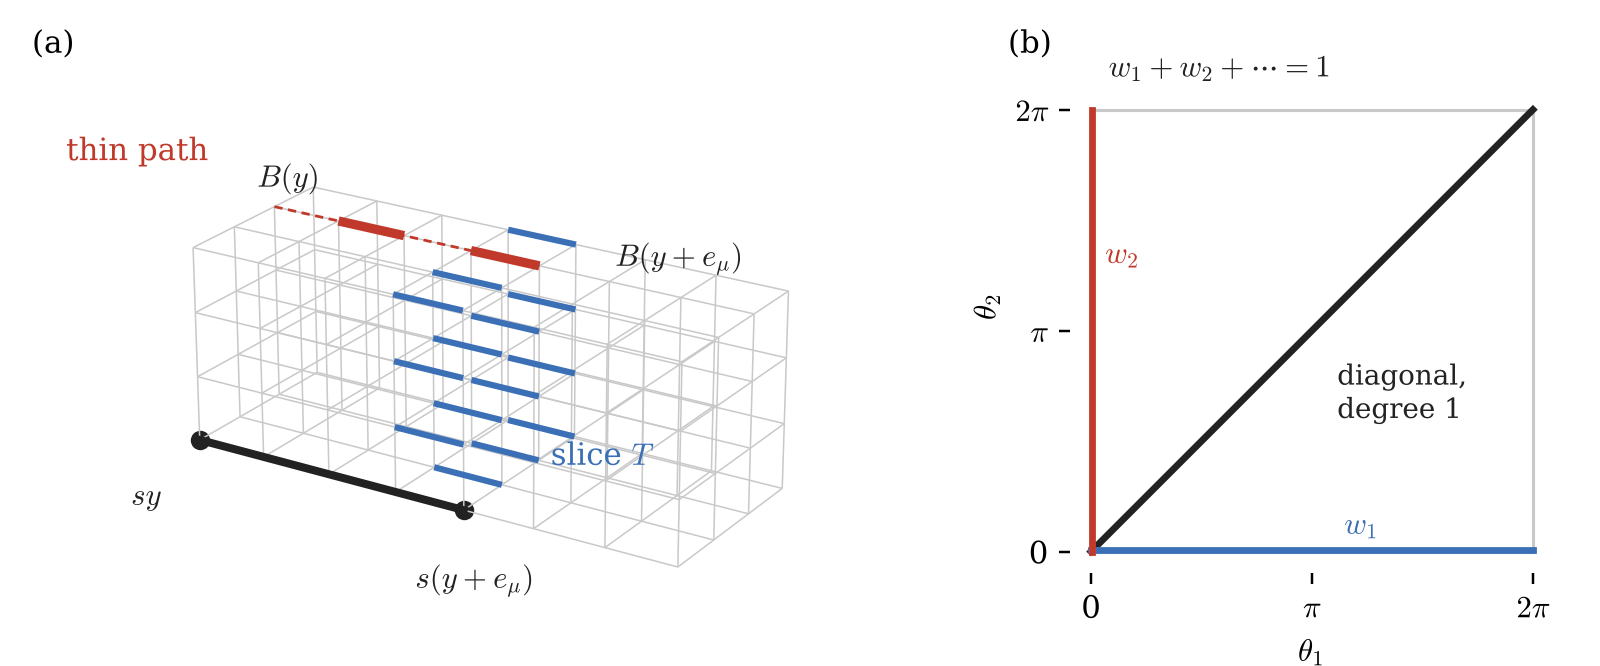
\includegraphics[width=0.9\textwidth]{figures/fig_pathblocks.png}
\caption{(a) Two adjacent blocks $B(y)$, $B(y+e_\mu)$ of side $s=4$, drawn
in three of the four dimensions. The black segment is the straight path
between the roots, the coarse link of the path map. The blue links form the
slice $T$ of Proposition~\ref{prop:nomean}. The red links carry the field of
Proposition~\ref{prop:thinpath}: a path whose holonomy is that of a coarse
link of order one, at a fine energy of order $1/s$. (b) For $\SU(2)$, two coordinates of
the torus $(\R/2\pi\Z)^T$ of slice fields with values in a maximal torus.
The diagonal is pure gauge and is sent to a loop of degree one, so the
degrees $W_t$ of the coordinate loops add up to one.}
\label{fig:pathblocks}
\end{figure*}

The proposition leaves room for a map that treats the positions alike to
first order and breaks the symmetry only where the field is large. For a
coarse link $(y,\mu)$ and $x\in B(y)$ put
\[
P_x=U_{x,\mu}U_{x+e_\mu,\mu},
\]
the product along the straight path of length two from $x$ to $x+2e_\mu$.
In the tree gauge it is the parallel transport from $2y$ to $2y+2e_\mu$
through $x$ and $x+2e_\mu$, it transforms as a link under the gauge
transformations at the block roots, and $P_{2y}=V^{\rm p}_{y,\mu}$, since
the first link of that path is a tree link. Let $\mathfrak g$ be the Lie
algebra of $G$, $\lVert X\rVert$ the Hilbert--Schmidt norm and $\log$ the
principal logarithm of unitary matrices without the eigenvalue $-1$.

\begin{lemma}\label{lem:logbound}
If $g$ is unitary and $\delta(g,I)\le1$, then $\lVert\log g\rVert\le\frac\pi
3\,\delta(g,I)$. If $X$ is skew-Hermitian, then $\delta(e^X,I)\le\lVert
X\rVert$.
\end{lemma}

\begin{proof}
Let $e^{i\theta_j}$, $|\theta_j|\le\pi$, be the eigenvalues of $g$. Then
$\delta(g,I)^2=\sum_j4\sin^2(\theta_j/2)$ and $\lVert\log g\rVert^2=\sum_j
\theta_j^2$. Each term of the first sum is at most $1$, so $|\theta_j|\le
\pi/3$, and $\theta/(2\sin(\theta/2))$ increases on $(0,\pi)$ and equals
$\pi/3$ at $\theta=\pi/3$. The second statement is $|e^{i\theta}-1|\le
|\theta|$ for the eigenvalues of $X$.
\end{proof}

Let $\rho_G\in(0,1]$ be such that $\log g\in\mathfrak g$ for every $g\in G$
with $\delta(g,I)\le\rho_G$.\footnote{The exponential map of $G$ is a
diffeomorphism from a ball of $\mathfrak g$ of operator-norm radius less than
$\pi$ onto a neighbourhood $N$ of $I$ in $G$, on which it inverts the
principal logarithm, and $N$ contains $\{g\in G:\delta(g,I)\le\rho\}$ for
small $\rho>0$. For $\U(r)$ one may take $\rho_G=1$. For $\SU(N)$ one may
take $\rho_G=\min\{1,5/\sqrt N\}$: by Lemma~\ref{lem:logbound} the trace of
$\log g$ has modulus at most $\sqrt N\,\pi\rho_G/3<2\pi$, and it lies in
$2\pi i\Z$. Some restriction is needed: on the circle $\{\operatorname{diag}
(z,z^7)\}\subset\U(2)$ the point $z=e^{2\pi i/7}$ has $\delta(g,I)<1$ but
$\log g\notin\mathfrak g$.} Let $\phi(t)=\min\{1,\max\{0,2-2t\}\}$, which
equals $1$ on $[0,\frac12]$ and $0$ on $[1,\infty)$, put
\[
\chi_{y,\mu}(U)=\phi\Bigl(\rho_G^{-1}\max_{x\in B(y)}\delta(P_x,P_{2y})
\Bigr),
\]
and define the \emph{cut-off average}
\begin{equation}\label{eq:cutoff}
V^\sharp_{y,\mu}(U)=P_{2y}\exp\Bigl(\frac{\chi_{y,\mu}(U)}{16}\sum_{x\in
B(y)}\log\bigl(P_{2y}^{-1}P_x\bigr)\Bigr),
\end{equation}
the exponential factor being $I$ when $\chi_{y,\mu}(U)=0$
(Fig.~\ref{fig:cutoff}). When every path is close to the straight one it is
the average of the sixteen paths taken in the chart at $P_{2y}$; when some
path is far from it, it is the path map.

\begin{figure*}[t]
\centering
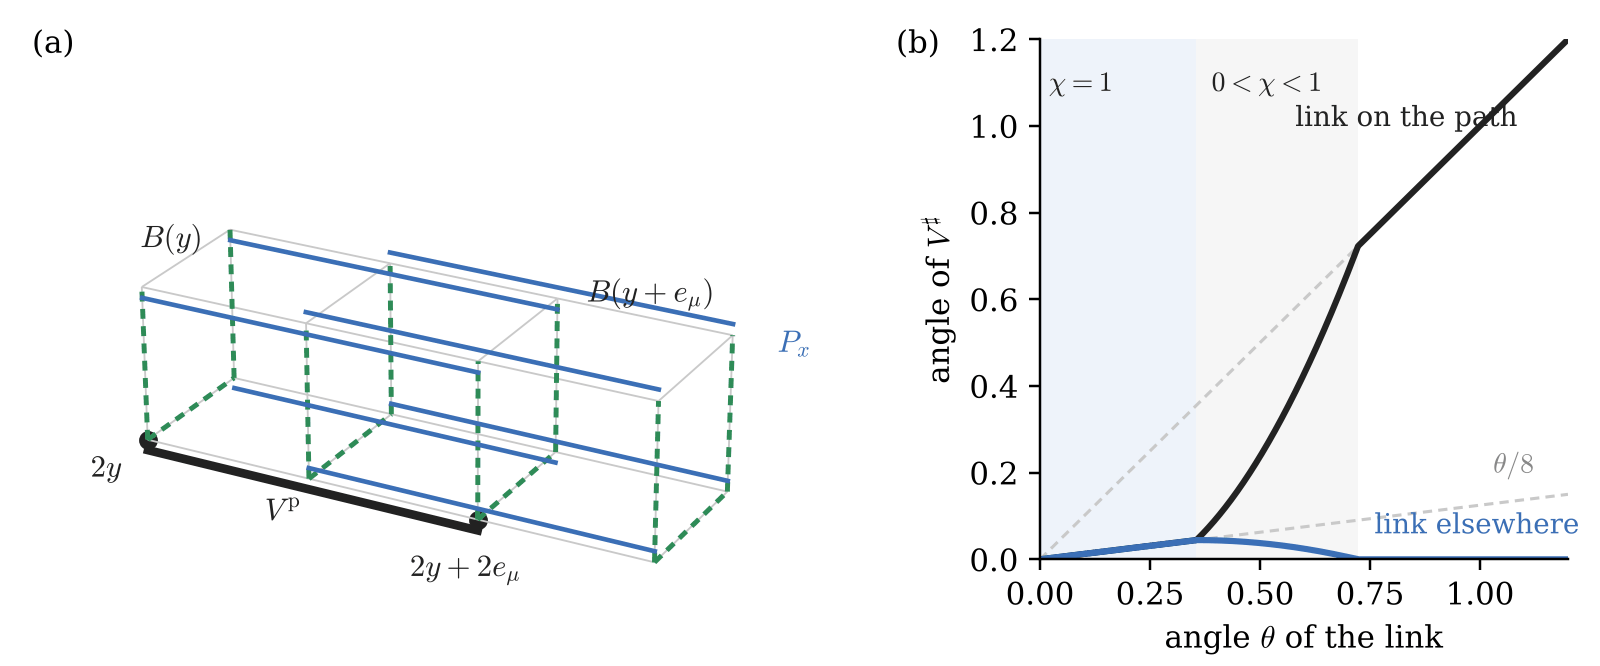
\includegraphics[width=0.9\textwidth]{figures/fig_cutoff.png}
\caption{(a) A block $B(y)$ of side two and the next block in the direction
$\mu$, drawn in three of the four dimensions. Green dashed: the tree links,
equal to $I$. Blue: the paths $P_x$ of length two from the sites of $B(y)$,
each joining $2y$ to $2y+2e_\mu$ through the trees; black: the straight path
$P_{2y}$, the coarse link of the path map. The cut-off average is the mean of
the sixteen paths in the chart at $P_{2y}$ while every path is close to it.
(b) For $\SU(2)$ and one link $e^{\theta X}$, $X=\operatorname{diag}(i,-i)$,
the angle of $V^\sharp$ when the link lies on the straight path (black) or at
another transverse position (blue), with $\rho_G=1$. Both equal $\theta/8$,
the block average, while $\chi=1$; past the cut-off they are the path map,
$\theta$ and $0$, so the slice windings are $1$ and $0$.}
\label{fig:cutoff}
\end{figure*}

\begin{theorem}\label{thm:cutoff}
For every compact $G\subset\U(r)$ the cut-off average is continuous,
covariant and normalised, and the following hold, with $c=\pi/3$.
\begin{enumerate}[label=\textup{(\roman*)},leftmargin=*]
\item If $\delta(P_x,P_{2y})\le\rho_G/2$ for every $x\in B(y)$, then
$V^\sharp_{y,\mu}(U)=P_{2y}\exp\bigl(\frac1{16}\sum_x\log(P_{2y}^{-1}P_x)
\bigr)$. For $\varphi$ with values in $\mathfrak g$, vanishing on the tree
links,
\[
V^\sharp_{y,\mu}(e^{t\varphi})=I+t\,V_{y,\mu}(\varphi)+O(t^2),
\]
with $V_{y,\mu}$ the block average of Definition~\ref{def:blockgauge}.
\item For every field $U$ in the tree gauge,
\begin{align*}
\sum_{y,\mu}\sum_{x\in B(y)}\delta(P_x,P_{2y})^2&\le896\,Q(U),\\
\sum_{y,\mu}\delta\bigl(V^\sharp_{y,\mu}(U),V^{\rm p}_{y,\mu}(U)\bigr)^2
&\le56c^2\,Q(U),\\
\sum_e\delta\bigl(U_e,R_e(V^\sharp(U))\bigr)^2&\le(448+896c^2)\,Q(U),\\
Q_1\bigl(V^\sharp(U)\bigr)&\le(8+2688c^2)\,Q(U),
\end{align*}
and $448+896c^2<1431$, $8+2688c^2<2956$.
\item In the setting of Proposition~\ref{prop:nomean} with $s=2$, $W_t$ is
the identity at the position of the straight path and $0$ at the seven
others.
\item If $U$ equals $I$ except on one link from $B(y)$ to $B(y+e_\mu)$,
where it equals $g$ with $\delta(g,I)\le\rho_G/2$, then $V^\sharp_{y,\mu}(U)=
\exp(\frac18\log g)$, at each of the eight transverse positions of the link;
the path map gives $g$ at one position and $I$ at the seven others.
\end{enumerate}
\end{theorem}

\begin{proof}
Write $P=P_{2y}$, $v_x=P^{-1}P_x$ and $m=\max_x\delta(v_x,I)=\max_x\delta(P_x
,P)$. Where $m<\rho_G$, every $\log v_x$ lies in $\mathfrak g$, depends
continuously on $U$ by Lemma~\ref{lem:logbound}, which keeps the eigenvalues
of $v_x$ away from $-1$, and the exponent of~\eqref{eq:cutoff} lies in
$\mathfrak g$, so $V^\sharp\in G$. Where $m\ge\rho_G$, $V^\sharp=P$. As $m$
increases to $\rho_G$ the exponent has norm at most $\chi c\rho_G\to0$, so
$V^\sharp$ is continuous. Let $h$ be a gauge transformation equal to $h_1$
on $B(y)$ and to $h_2$ on $B(y+e_\mu)$. The middle point $x+e_\mu$ of each
path lies in one of the two blocks, so $P_x\mapsto h_1P_xh_2^{-1}$ and
$v_x\mapsto h_2v_xh_2^{-1}$; $\delta$ is invariant and $\log$ is equivariant
under unitary conjugation, so $\chi$ is unchanged and $V^\sharp\mapsto h_1
V^\sharp h_2^{-1}$. At $U=I$ every $v_x$ is $I$, so $V^\sharp(I)=I$.

(i) The first statement is $\chi=1$. If $U=e^{t\varphi}$ with $\varphi=0$ on
the tree, then $P=I+t\varphi_{2y+e_\mu,\mu}+O(t^2)$ and
$\log v_x=t(\varphi_{x,\mu}+\varphi_{x+e_\mu,\mu}-\varphi_{2y+e_\mu,\mu})+
O(t^2)$, and for small $t$ the condition of the first statement holds. The
mean over the sixteen $x$ is $t(V_{y,\mu}(\varphi)-\varphi_{2y+e_\mu,\mu})
+O(t^2)$, since $\varphi_{2y,\mu}=0$, and multiplying by $P$ gives the
claim.

(ii) In the tree gauge $P=v_{y,\mu}:=V^{\rm p}_{y,\mu}(U)$. If $o_\mu=0$,
then $U_{x+e_\mu,\mu}$ is the link leaving $B(y)$ at the transverse offset of
$x$, and invariance of $\delta$ with the triangle inequality gives
$\delta(P_x,P)\le\delta(U_{x,\mu},I)+\delta(U_{x+e_\mu,\mu},v_{y,\mu})$; if
$o_\mu=1$, the roles of the two links are exchanged. Each link leaving a
block in the direction $\mu$ occurs for two sites $x$ of that block, and
each link in the direction $\mu$ with $o_\mu=0$ occurs once for the block
containing it and once for the block before it. With $(a+b)^2\le2a^2+2b^2$
and the notation of the proof of Theorem~\ref{thm:pathcoercive}, the sum is
at most $2(2I_0+2J_0)=4D_v^2\le896Q$. Next, if $\chi>0$,
Lemma~\ref{lem:logbound} and the Cauchy--Schwarz inequality give
\begin{align*}
\delta(V^\sharp,P)&\le\Bigl\lVert\frac\chi{16}\sum_x\log v_x\Bigr\rVert\le
\frac c{16}\sum_x\delta(v_x,I)\\
&\le\frac c4\Bigl(\sum_x\delta(P_x,P)^2\Bigr)^{1/2},
\end{align*}
and the second bound follows from the first, $896c^2/16=56c^2$. The
reconstruction $R(V^\sharp)$ agrees with $R(v)$ on the links with $o_\mu=0$,
and on the eight links with $o_\mu=1$ of each block and direction
$\delta(U_e,V^\sharp)^2\le2\delta(U_e,v)^2+2\delta(V^\sharp,v)^2$; so the
third sum is at most $2D_v^2+16\cdot56c^2Q\le(448+896c^2)Q$. Finally, write
$V^\sharp=vM$. Removing the four factors $M$ from the holonomy of a coarse
plaquette one at a time changes $\delta(\cdot,I)$ by at most $\delta(M,I)$
each time, so $\delta(V^\sharp_P,I)^2\le2\delta(v_P,I)^2+8\sum_{\ell\in P}
\delta(M_\ell,I)^2$. Each coarse link lies in six coarse plaquettes, so
$Q_1(V^\sharp)\le2Q_1(v)+48\cdot56c^2Q$, and $Q_1(v)\le4Q$ by
Proposition~\ref{prop:pathenergy}. The numerical bounds use $c^2<1.0967$.

(iii) For $s=2$ the slice $T$ consists of the eight links leaving $B(y)$,
and the links inside the blocks are $I$, so $P_x=u_{a}$ for the transverse
offset $a$ of $x$, two sites for each $a$. Let $t$ be a position other than
the straight path and $u_{t'}=I$ for $t'\ne t$. Then $P=I$, two of the
$v_x$ equal $u_t$ and the others $I$, so $F(u)=\exp(\frac18\chi\log u_t)$
with $\chi=\phi(\delta(u_t,I)/\rho_G)$. On $S$ the maps
$u_t\mapsto\exp(\frac\lambda8\chi\log u_t)$, $0\le\lambda\le1$, are
continuous by the argument above and take values in $S$, since $\log u_t$
commutes with $S$ and the centraliser of a maximal torus in $\mathfrak g$ is
its Lie algebra; they join $F$ to the constant $I$, so
$W_t=0$. By Proposition~\ref{prop:nomean} the $W_t$ add up to the identity,
which is therefore the matrix at the straight path.

(iv) At the straight path, $P_x=g$ for the two sites with transverse offset
$0$ and $P_x=I$ for the others, so $V^\sharp=g\exp(-\frac{14}{16}\log g)=
\exp(\frac18\log g)$; at another position, $P=I$ and two of the $P_x$ equal
$g$, so $V^\sharp=\exp(\frac2{16}\log g)$.
\end{proof}

The small-field part of~\eqref{eq:cutoff} is Ba{\l}aban's averaging
operation~\cite{Bal85a}; the cut-off extends it to all fields with the
bounds of (ii). The theorem shows how far Proposition~\ref{prop:nomean}
reaches. The cut-off average is continuous, covariant and coercive for
every field, and it agrees with the block averages to first order. Its slice
windings are those of the path map, as the proposition demands of any such
map, but the departure from the transverse symmetry happens only where some
path differs from the straight one by more than $\rho_G/2$. Below that the
field of a single link enters with the weight $\frac18$ of the averages,
whichever position it occupies.

What the theorem does not give is composition. The constants of (ii) are
those of one step, and iterating them gives a factor that grows
exponentially in the number of steps; on its large-field branch the map is
the path map, for which Proposition~\ref{prop:thinpath} rules out any bound
uniform in that number. Whether the $k$-fold cut-off average obeys
$Q_k(V^{\sharp,k}(U))\le C\,Q(U)$ and the corresponding coercivity bound
with $C$ independent of $k$ is open for general fields; it is the form in
which Remark~\ref{rem:constrainedopen}(b) remains. Section~\ref{ssec:scales}
proves it, with $C=1.001$, for fields with values in a maximal torus whose
curvature stays small at every scale, and with $C=e^{12060\sigma}$ for fields
of any compact group whose curvatures at the successive scales are small with
sum $\sigma$.

\subsection{Composition across scales}\label{ssec:scales}

This subsection proves that the cut-off average composes across all scales
on fields with values in a maximal torus whose curvature stays small, which
includes the thin paths that defeat the path map, and then that it
composes for every compact group on fields whose curvature is small, with
a summable loss over the scales.

\begin{figure*}[t]
\centering
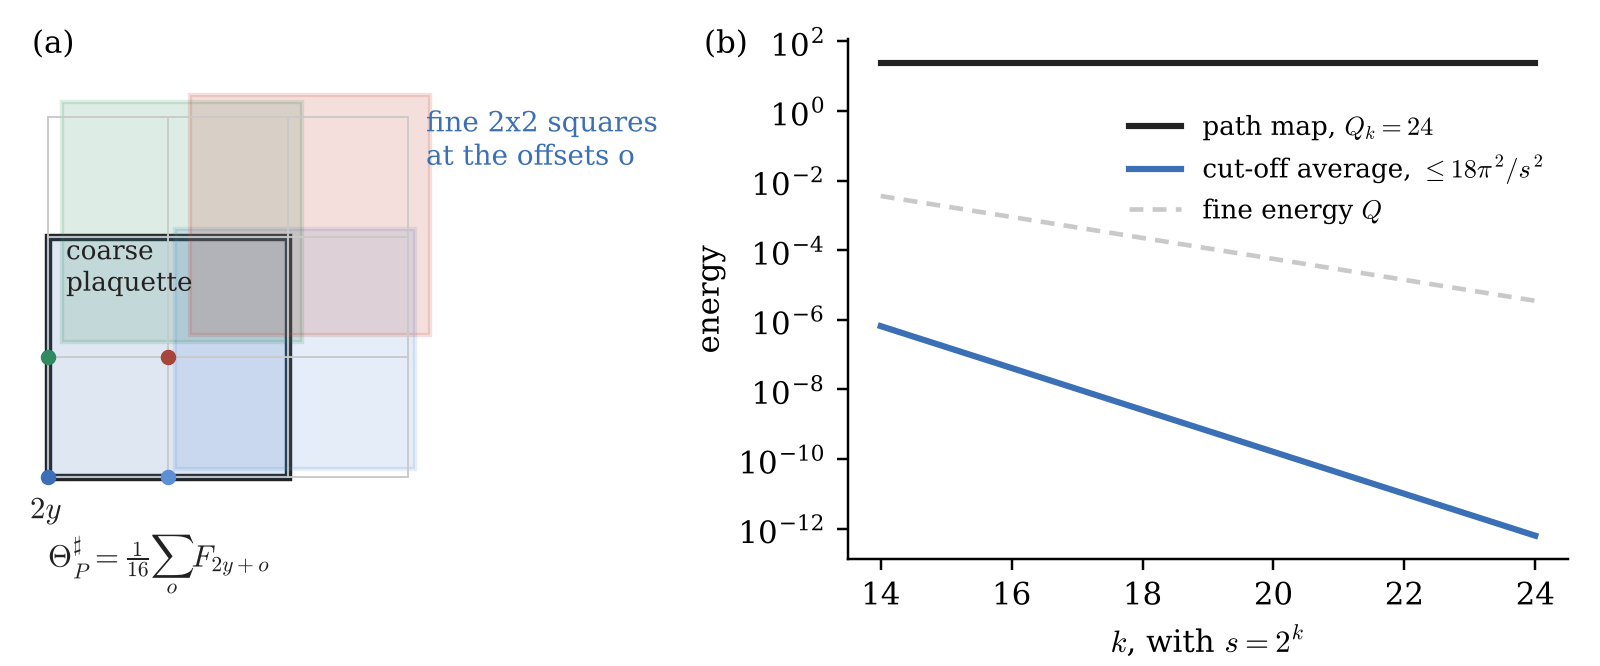
\includegraphics[width=0.9\textwidth]{figures/fig_scales.png}
\caption{(a) In the torus, the coarse plaquette of the cut-off average is
the mean of the fluxes $F_{2y+o}$ of the sixteen fine squares of side two
at the offsets $o$ (four of them drawn), whatever the gauge of the coarse
links (Lemma~\ref{lem:torusstep}). (b) For the thin-path fields of
Proposition~\ref{prop:thinpath}, the coarse energy after $k$ steps: $24$
for the path map, at most $18\pi^2/s^2$ for the cut-off average
(Corollary~\ref{cor:thinscales}); the fine energy is about $6\pi^2/s$.}
\label{fig:scales}
\end{figure*}

Let $S$ be a maximal torus of $G\subset\U(r)$ and $\mathfrak s$ its Lie
algebra. The exponential maps $\mathfrak s$ onto $S$, and its kernel
$\Lambda$ consists of diagonalisable matrices with eigenvalues in $2\pi i\Z$,
so every nonzero element of $\Lambda$ has norm at least $2\pi$. For an
$S$-valued field with $\delta(U_p,I)\le\rho_G$ on every plaquette put
$\Theta_p=\log U_p$; it lies in $\mathfrak g$, commutes with $S$, and so
lies in $\mathfrak s$. For a fine site $x$ and a coordinate plane $\{\mu,\nu
\}$ let $\square_x$ be the square of side two at $x$ in that plane and
$F_x=\sum_{p\subset\square_x}\Theta_p$, the sum of its four plaquettes,
oriented as the square. Put
\[
\eta_G=\rho_G/12.
\]
The $k$-fold cut-off average is defined by putting the coarse field back
into the tree gauge, by an $S$-valued gauge transformation, before each
step. The tree gauge fixes such a transformation up to one that is constant
on blocks, under which $V^\sharp$ is covariant, so the coarse plaquette
holonomies $U^{(j)}_P$ of the $j$-th iterate $U^{(j)}$ are well defined; we
write $\Theta^{(j)}_P=\log U^{(j)}_P$ when $\delta(U^{(j)}_P,I)\le\rho_G$.

\begin{lemma}\label{lem:torusstep}
Let $U$ be an $S$-valued field in the tree gauge with $\lVert\Theta_p\rVert
\le\eta_G$ for every plaquette. Then $\chi_{y,\mu}(U)=1$ for every coarse
link, and the coarse plaquette $P$ at $y$ in the plane $\{\mu,\nu\}$ has
\[
V^\sharp(U)_P=\exp\bar F_P,\qquad\bar F_P=\frac1{16}\sum_{o\in\{0,1\}^4}
F_{2y+o},
\]
with $\lVert\bar F_P\rVert\le4\max_p\lVert\Theta_p\rVert$, so that $\log
V^\sharp(U)_P=\bar F_P$.
\end{lemma}

\begin{proof}
Let $\eta=\max_p\lVert\Theta_p\rVert$. Fix $(y,\mu)$ and $x=2y+o$. The tree
path $\tau$ from $2y$ to $x$ sets the coordinates of $o$ one at a time in
increasing order, so it has at most four edges, at most three of them
transverse to $\mu$. In the tree gauge its links are $I$, so
$P_{2y}^{-1}P_x$ is the holonomy of the loop $\tau$, then the straight path
from $x$ to $x+2e_\mu$, then $\tau+2e_\mu$ backwards, then the straight path
from $2y+2e_\mu$ back to $2y$. This loop is the boundary of the surface
swept by the transverse edges of $\tau$ along two steps in the direction
$\mu$: at most six distinct plaquettes, each with coefficient $\pm1$. The
group is abelian, so $P_{2y}^{-1}P_x=\exp d_x$ with $d_x$ the signed sum of
their $\Theta_p$, and $\lVert d_x\rVert\le6\eta\le\rho_G/2$. By
Lemma~\ref{lem:logbound}, $\delta(P_x,P_{2y})\le\rho_G/2$, so $\chi=1$, and
since the eigenvalues of $d_x$ have modulus at most $\frac12$,
$\log(P_{2y}^{-1}P_x)=d_x$. Hence $V^\sharp_{y,\mu}=\exp(X_{y,\mu}+\bar
d_{y,\mu})$, where $X_{y,\mu}\in\mathfrak s$ is any logarithm of $P_{2y}$
and $\bar d_{y,\mu}$ is the mean of the $d_x$.

Let the sides of $P$ be the coarse links $\ell$ with signs $\epsilon_\ell$,
and write $d_{o,\ell}$ for the $d_x$ of the side $\ell$ at the offset $o$.
For each $o$ the four straight paths of length two at the offset $o$ of the
four sides bound the square $\square_{2y+o}$, so
\[
Y_o=\sum_\ell\epsilon_\ell\bigl(X_\ell+d_{o,\ell}\bigr)-F_{2y+o}\in
\Lambda .
\]
Since $d_{0,\ell}=0$, $\lVert Y_o-Y_0\rVert\le4\cdot6\eta+8\eta=32\eta\le
\frac83<2\pi$, so $Y_o=Y_0$ for every $o$. Averaging over $o$ gives
$\sum_\ell\epsilon_\ell(X_\ell+\bar d_\ell)=\bar F_P+Y_0$, and $\exp Y_0=I$.
Finally $\lVert\bar F_P\rVert\le\max_o\lVert F_{2y+o}\rVert\le4\eta<\pi/3$,
so $\bar F_P$ is the principal logarithm.
\end{proof}

\begin{theorem}\label{thm:torusscales}
Let $U$ be an $S$-valued field in the tree gauge on the periodic lattice of
side divisible by $2^k$, with $\delta(U_p,I)\le\rho_G$ on every plaquette,
and put $\eta_0=\max_p\lVert\Theta_p\rVert$, $A=\sum_p\lVert\Theta_p\rVert$.
Suppose that
\begin{equation}\label{eq:torushyp}
\max_P\lVert\Theta^{(j)}_P\rVert\le\eta_G\quad\text{for }0\le j<k,
\end{equation}
which holds in particular if $\eta_0A\le\eta_G^2$. Then the cut-off is
inactive at every step, $\Theta^{(j+1)}=\bar F(\Theta^{(j)})$, and for
$j<k$
\begin{gather*}
\sum_P\lVert\Theta^{(j+1)}_P\rVert^2\le\sum_P\lVert\Theta^{(j)}_P\rVert^2,
\qquad\sum_P\lVert\Theta^{(j+1)}_P\rVert\le\frac14\sum_P\lVert
\Theta^{(j)}_P\rVert,\\
\max_P\lVert\Theta^{(j+1)}_P\rVert\le4\max_P\lVert\Theta^{(j)}_P\rVert.
\end{gather*}
Consequently
\begin{align*}
Q_k\bigl(V^{\sharp,k}(U)\bigr)&\le\sum_p\lVert\Theta_p\rVert^2\le1.001\,
Q(U),\\
Q_k\bigl(V^{\sharp,k}(U)\bigr)&\le16^{-k}A^2 .
\end{align*}
\end{theorem}

\begin{proof}
The first assertions follow from Lemma~\ref{lem:torusstep} by induction,
the $S$-valued gauge fixing between steps leaving the plaquette holonomies
unchanged. The coarse plaquettes $P$ in a plane together with the offsets
$o$ are in bijection with the fine squares $\square_x$ in that plane,
$x=2y+o$, and a fine plaquette lies in four such squares. With $\lVert\bar
F_P\rVert^2\le\frac1{16}\sum_o\lVert F_{2y+o}\rVert^2$ and $\lVert F_x
\rVert^2\le4\sum_{p\subset\square_x}\lVert\Theta_p\rVert^2$ this gives
$\sum_P\lVert\bar F_P\rVert^2\le\frac1{16}\cdot4\cdot4\sum_p\lVert\Theta_p
\rVert^2$; the same count without Cauchy--Schwarz gives the factor
$\frac14$ in the second inequality, and the third is $\lVert F_x\rVert\le
4\eta$.

For the sufficient condition, let $\eta_j$ and $A_j$ be the maximum and the
sum of $\lVert\Theta^{(j)}_P\rVert$. While~\eqref{eq:torushyp} holds up to
$j-1$, the inequalities give $\eta_j\le4^j\eta_0$ and $\eta_j\le A_j\le
4^{-j}A$. The product of the two bounds is $\eta_0A\le\eta_G^2$, so the
smaller one is at most $\eta_G$, and~\eqref{eq:torushyp} holds at $j$.

Finally $\delta(\exp\Theta,I)\le\lVert\Theta\rVert$
(Lemma~\ref{lem:logbound}), so $Q_k(V^{\sharp,k}(U))\le\sum_P\lVert
\Theta^{(k)}_P\rVert^2$, which is at most both $\sum_p\lVert\Theta_p
\rVert^2$ and $\eta_kA_k\le A_k^2\le16^{-k}A^2$. The eigenvalues of each
$\Theta_p$ are $i\theta$ with $|\theta|\le\eta_0\le\eta_G\le\frac1{12}$, since
$\eta_0^2\le\eta_0A$ in the sufficient condition and $\eta_0\le\eta_G$ is
the case $j=0$ of~\eqref{eq:torushyp}; and $\theta^2\le1.001\cdot4\sin^2(
\theta/2)$ there, which gives $\sum_p\lVert\Theta_p\rVert^2\le1.001\,Q(U)$.
\end{proof}

\begin{corollary}\label{cor:thinscales}
For $G=\SU(2)$ and the fields of Proposition~\ref{prop:thinpath} with
$s=2^k\ge2^{14}$,
\begin{align*}
Q_k\bigl(V^{\sharp,k}(U)\bigr)&\le\frac{18\pi^2}{s^2}\le\frac4s\,Q(U),\\
Q_k\bigl(V^{{\rm p},k}(U)\bigr)&=24\ge\frac{4s}{\pi^2}\,Q(U).
\end{align*}
\end{corollary}

\begin{proof}
Here $\rho_G=1$ and $S$ is the diagonal torus. The $3s$ nonzero plaquettes
have $\Theta_p=\pm2T/s$, of norm $\sqrt2\pi/s$, so $\eta_0A=6\pi^2/s\le
\frac1{144}$ when $s\ge864\pi^2$, which holds for $s\ge2^{14}$, and $A^2=
18\pi^2$. Proposition~\ref{prop:thinpath} gives $Q(U)=24s\sin^2(\pi/2s)$,
which lies between $(6\pi^2/s)(1-\pi^2/(12s^2))$ and $6\pi^2/s$.
\end{proof}

So on torus-valued fields of small curvature the cut-off average behaves
like the linear averages: the curvature is averaged over the sixteen
offsets at every step, the energy never increases, and a thin path is
spread out and contracted instead of being carried to the coarse lattice
(Fig.~\ref{fig:scales}).

For general fields the paths do not commute, and the logarithms carry
commutators from the second order on. The next two lemmas bound these
commutators by the square of the local curvature. The same composition
then holds for every compact group, with a loss of at most $1+O(\eta_j)$ at
scale $j$.

\begin{lemma}\label{lem:bch}
Let $Z_1,\dots,Z_n\in\mathfrak g$ with $r=\sum_i\lVert Z_i\rVert\le\min\{
\frac14,\rho_G\}$, and let $g=e^{Z_1}\cdots e^{Z_n}$. Then $\delta(g,I)\le
r$, $\log g\in\mathfrak g$, and
\[
\Bigl\lVert\log g-\sum_iZ_i\Bigr\rVert\le1.6\,r^2 .
\]
\end{lemma}

\begin{proof}
The distance $\delta$ is invariant under multiplication by unitary
matrices on either side, so $\delta(g,I)\le\sum_i\delta(e^{Z_i},I)\le r$ by
Lemma~\ref{lem:logbound}, and $\log g\in\mathfrak g$ by the choice of
$\rho_G$. Expanding the exponentials, $g-I-\sum_iZ_i$ is a sum of products
of at least two factors. Since the Hilbert--Schmidt norm is
submultiplicative, its norm is at most $e^r-1-r\le\frac12r^2e^r\le0.643\,
r^2$, and $M=g-I$ has $\lVert M\rVert\le e^r-1\le1.137\,r\le0.285$. The
operator norm of $M$ is smaller than $1$. The principal logarithm is
holomorphic on the disc $|z-1|<1$, which contains the spectrum of $g$,
so it is given there by its power series, $\log g=\sum_{k\ge1}(-1)^{k+1}
M^k/k$. Hence
\[
\lVert\log g-M\rVert\le\frac{\lVert M\rVert^2}{2(1-\lVert M\rVert)}\le
0.905\,r^2 ,
\]
and the two bounds add up to less than $1.6\,r^2$.
\end{proof}

Let $U$ be a $G$-valued field in the tree gauge with $\delta(U_p,I)\le
\rho_G$, and put $\Theta_p=\log U_p$. A change of base point conjugates
$\Theta_p$ and does not change its norm. Let $P$ be a coarse plaquette at $y$
in the plane $\{\mu,\nu\}$. Its sides are $\ell_1=(y,\mu)$, $\ell_2=(y+
e_\mu,\nu)$, $\ell_3=(y+e_\nu,\mu)$ and $\ell_4=(y,\nu)$, with initial
points $y_i$. For an offset $o\in\{0,1\}^4$ let $P_{i,o}$ be the path
product of $\ell_i$ through $2y_i+o$, and put
\[
K_{P,o}=P_{1,o}P_{2,o}P_{3,o}^{-1}P_{4,o}^{-1},\qquad\bar F_P=\frac1{16}
\sum_o\log K_{P,o}.
\]
The tree segments between consecutive sides cancel. Hence $K_{P,o}$ is the
holonomy of the square $\square_{2y+o}$, carried to $2y$ along the tree.
In a torus, $\log K_{P,o}=F_{2y+o}$, and $\bar F_P$ is the mean of
Lemma~\ref{lem:torusstep}. Let $\sigma_{P,o}$ be the sum of $\lVert
\Theta_p\rVert$ over the four plaquettes of $\square_{2y+o}$.

\begin{lemma}\label{lem:smallstep}
Let $U$ be a $G$-valued field in the tree gauge with $\delta(U_p,I)\le
\rho_G$ and $\lVert\Theta_p\rVert\le\eta\le\rho_G/1000$ for every
plaquette. Then $\chi_{y,\mu}(U)=1$ for every coarse link. Every coarse
plaquette has $\delta(V^\sharp(U)_P,I)\le0.03\,\rho_G$ and
\begin{equation}\label{eq:smallstep}
\begin{aligned}
\bigl\lVert\log V^\sharp(U)_P-\bar F_P\bigr\rVert&\le3.2\,r_P^2,\\
\lVert\bar F_P\rVert&\le\frac{1+6.4\eta}{16}\sum_o\sigma_{P,o},
\end{aligned}
\end{equation}
with $r_P\le28.26\,\eta$ defined in the proof. Let $E$, $A$ be the sum of
$\lVert\Theta_p\rVert^2$ and of $\lVert\Theta_p\rVert$, and let $E'$, $A'$,
$\eta'$ be the sum of squares, the sum and the maximum of $\lVert\log
V^\sharp(U)_P\rVert$. Then
\begin{gather*}
\sqrt{E'}\le(1+6030\eta)\sqrt E,\qquad A'\le(1+9147\eta)\frac A4,\\
\eta'\le4(1+647\eta)\,\eta .
\end{gather*}
\end{lemma}

\begin{proof}
\emph{Paths.} Fix a coarse link $(y,\mu)$ and $x=2y+o$. As in the proof of
Lemma~\ref{lem:torusstep}, $P_{2y}^{-1}P_x$ is the holonomy of a loop
bounding a surface of at most six plaquettes, swept by the transverse edges
of the tree path. Build the surface one plaquette at a time. This writes
the holonomy as a product of at most six factors $hU_p^{\pm1}h^{-1}=
\exp(\pm h\Theta_ph^{-1})$. Let $\sigma_{(y,\mu),o}\le6\eta$ be the sum of
their $\lVert\Theta_p\rVert$. By Lemma~\ref{lem:bch}, $\delta(P_x,P_{2y})
\le6\eta\le\rho_G/2$, so $\chi=1$. The logarithm $D_{(y,\mu),o}=\log(
P_{2y}^{-1}P_x)$ lies in $\mathfrak g$, with
\[
\lVert D_{(y,\mu),o}\rVert\le(1+9.6\eta)\,\sigma_{(y,\mu),o}.
\]
In the same way $K_{P,o}$ is a product of four such factors, so
$\lVert\log K_{P,o}\rVert\le(1+6.4\eta)\sigma_{P,o}$. Averaging over $o$
gives the second inequality of~\eqref{eq:smallstep}.

\emph{The plaquette.} Write $D_{i,o}$ for $D_{\ell_i,o}$. Then $P_{i,o}=
P_{i,0}e^{D_{i,o}}$ and $D_{i,0}=0$, and $V^\sharp_{\ell_i}=P_{i,0}
e^{m_i}$ with $m_i=\frac1{16}\sum_oD_{i,o}$. The paths and $V^\sharp$
transform as links under gauge transformations constant on blocks. These
transformations preserve the tree gauge and conjugate $D_{i,o}$, $m_i$,
$K_{P,o}$ and $V^\sharp_P$ by fixed elements. Choose one with $P_{1,0}=
P_{2,0}=P_{3,0}=I$. Then $P_{4,0}=K_{P,0}^{-1}$, and with $c=\log
K_{P,0}$,
\begin{align*}
V^\sharp_P&=e^{m_1}e^{m_2}e^{-m_3}e^{-m_4}e^{c},\\
K_{P,o}&=e^{D_{1,o}}e^{D_{2,o}}e^{-D_{3,o}}e^{-D_{4,o}}e^{c}.
\end{align*}
Put $r_P=\sum_i\max_o\lVert D_{i,o}\rVert+\lVert c\rVert$. Since
$\lVert m_i\rVert\le\max_o\lVert D_{i,o}\rVert$, the five exponents in
each product have norms adding up to at most $r_P$, and
\[
r_P\le24(1+9.6\eta)\eta+4(1+6.4\eta)\eta\le28.26\,\eta .
\]
Lemma~\ref{lem:bch} gives $\delta(V^\sharp_P,I)\le r_P\le0.03\,\rho_G$ and
\begin{align*}
\log V^\sharp_P&=m_1+m_2-m_3-m_4+c+R,\\
\log K_{P,o}&=D_{1,o}+D_{2,o}-D_{3,o}-D_{4,o}+c+R_o,
\end{align*}
with $\lVert R\rVert,\lVert R_o\rVert\le1.6\,r_P^2$. Average the second
line over $o$ and subtract it from the first; since $m_i$ is the mean of
the $D_{i,o}$, this is the first inequality of~\eqref{eq:smallstep}.

\emph{Sums.} Each fine plaquette lies in four squares $\square_x$, and the
pairs $(P,o)$ are in bijection with these squares. The second inequality
of~\eqref{eq:smallstep} and Cauchy--Schwarz therefore give $\sum_P\lVert
\bar F_P\rVert^2\le(1+6.4\eta)^2E$; without Cauchy--Schwarz they give
$\sum_P\lVert\bar F_P\rVert\le(1+6.4\eta)A/4$. For the remainders, let
$\mathcal U_\ell$ be the set of plaquettes of the surfaces of the side
$\ell=(y,\mu)$ for all sixteen offsets. These lie in planes $\{\mu,\alpha
\}$, $\alpha\ne\mu$, at $\mu$-positions $2y_\mu$, $2y_\mu+1$, $2y_\mu+2$,
and there are at most $36$ of them. A plaquette lies in $\mathcal U_\ell$
for at most four coarse links. With $m'_\ell=\sum_{p\in\mathcal U_\ell}
\lVert\Theta_p\rVert$,
\[
r_P\le1.0096\Bigl(\sum_{\ell\subset P}m'_\ell+\sigma_{P,0}\Bigr).
\]
A coarse link is a side of six coarse plaquettes, and a plaquette lies in
$\square_{2y}$ for at most one coarse plaquette. Therefore
\begin{align*}
\sum_Pr_P&\le1.0096\,(6\cdot4A+A)\le25.24\,A,\\
\sum_Pr_P^2&\le1.0096^2\cdot5\,(6\cdot36\cdot4\,E+4E)\le4424\,E.
\end{align*}
Hence, with $r_P\le28.26\,\eta$,
\begin{align*}
\sum_P3.2\,r_P^2&\le3.2\cdot28.26\cdot25.24\,\eta A\le2283\,\eta A,\\
\Bigl(\sum_P\bigl(3.2\,r_P^2\bigr)^2\Bigr)^{1/2}&\le3.2\cdot28.26\,
\eta\,(4424\,E)^{1/2}\le6015\,\eta\sqrt E .
\end{align*}
The triangle inequality, for the Euclidean norm over
$P$ in the first case, gives $\sqrt{E'}\le(1+6.4\eta+6015\eta)\sqrt E$ and
$A'\le(1+6.4\eta)A/4+2283\,\eta A$. For the maximum, $\eta'\le(1+6.4\eta)
4\eta+3.2\,(28.26\,\eta)^2\le4(1+647\eta)\eta$.
\end{proof}

For a $G$-valued field, the $k$-fold cut-off average is defined as before,
with $G$-valued gauge transformations. The tree gauge fixes them up to
transformations constant on blocks, under which $V^\sharp$ is covariant.
These transformations conjugate the plaquette holonomies and leave the
norms $\lVert\Theta^{(j)}_P\rVert$ unchanged.

\begin{theorem}\label{thm:smallscales}
Let $G\subset\U(r)$ be compact and let $U$ be a $G$-valued field on the
periodic lattice of side divisible by $2^k$, with $\delta(U_p,I)\le\rho_G$
on every plaquette. Let $\eta_j$, $A_j$, $E_j$ be the maximum, the sum and
the sum of squares of $\lVert\Theta^{(j)}_P\rVert$ over the plaquettes of
the $j$-th iterate.
\begin{enumerate}[label=\textup{(\roman*)},leftmargin=*]
\item If $\eta_j\le\rho_G/1000$ for $0\le j<k$, the cut-off is inactive at
every step. With $\sigma=\sum_{j<k}\eta_j$,
\begin{gather*}
E_k\le e^{12060\sigma}E_0,\qquad A_k\le e^{9147\sigma}4^{-k}A_0,\\
\eta_k\le e^{647\sigma}4^k\eta_0 .
\end{gather*}
\item If $\eta_0A_0\le2\cdot10^{-10}\rho_G^2$, then (i) applies for every
$k$ with $\sigma\le7.25\sqrt{\eta_0A_0}$, and
\begin{align*}
Q_k\bigl(V^{\sharp,k}(U)\bigr)&\le e^{8.8\cdot10^4\sqrt{\eta_0A_0}}E_0
\le1.0001\,e^{8.8\cdot10^4\sqrt{\eta_0A_0}}\,Q(U),\\
Q_k\bigl(V^{\sharp,k}(U)\bigr)&\le e^2\,16^{-k}A_0^2 .
\end{align*}
\end{enumerate}
\end{theorem}

\begin{proof}
(i) Apply Lemma~\ref{lem:smallstep} at each step to the field in the tree
gauge; the gauge fixing does not change the norms. The lemma gives
$\delta(U^{(j+1)}_P,I)\le\rho_G$, so $\Theta^{(j+1)}$ is defined, and with
$1+t\le e^t$ the three inequalities of the lemma multiply over the steps.

(ii) Suppose that for $i<j$ we have $\eta_i\le\rho_G/1000$ and $\sum_{i<j}
\eta_i\le7.25\sqrt{\eta_0A_0}\le1/9747$. Then (i) gives $A_j\le e\,4^{-j}
A_0$ and $\eta_j\le e\,4^j\eta_0$, and $\eta_j\le A_j$. So $\eta_j\le e\min
\{4^j\eta_0,4^{-j}A_0\}\le e\sqrt{\eta_0A_0}\le\rho_G/1000$. Let $i_*$ be the
last index with $4^{i_*}\eta_0\le4^{-i_*}A_0$. The terms of $\min\{4^i\eta_0,
4^{-i}A_0\}$ increase by the factor $4$ up to $i_*$ and decrease by the
factor $4$ after it. The terms at $i_*$ and $i_*+1$ are at most $\sqrt{
\eta_0A_0}$, so the sum over all $i$ is at most $\frac83\sqrt{\eta_0A_0}$,
and $\sum_{i\le j}\eta_i\le\frac{8e}3\sqrt{\eta_0A_0}\le7.25\sqrt{\eta_0
A_0}$. This completes the induction. Then $E_k\le e^{12060\cdot7.25\sqrt{
\eta_0A_0}}E_0$. By Lemma~\ref{lem:logbound}, $Q_k(V^{\sharp,k}(U))\le E_k$,
and $E_k\le\eta_kA_k\le A_k^2\le e^2\,16^{-k}A_0^2$. Finally the eigenvalues
$i\theta$ of each $\Theta_p$ have $|\theta|\le\eta_0\le\sqrt{\eta_0A_0}<
10^{-4}$, and $\theta^2\le1.0001\cdot4\sin^2(\theta/2)$ there.
\end{proof}

For a torus Theorem~\ref{thm:torusscales} is sharper, and its hypothesis is
weaker; the content of Theorem~\ref{thm:smallscales} is the non-abelian
case. Neither theorem gives the
supremum over boundary conditions in (D). Theorem~\ref{thm:cutoff} has the
constants of one step. Theorems~\ref{thm:torusscales}
and~\ref{thm:smallscales} need the curvature to be small at every scale:
in Theorem~\ref{thm:smallscales} the losses $e^{6030\eta_j}$ must have a
bounded product, and a field whose curvature is smooth on a scale $\ell$
grows by a factor four per step until the coarse spacing reaches $\ell$.
The large fields, where the cut-off is active, and the Wilson measure
itself are outside both; Sec.~\ref{ssec:largefields} shows where the large
fields lie under that measure.



\subsection{Small fields on the fibres of the cut-off average}\label{ssec:smallfibres}

Theorem~\ref{thm:blockgap} is a gap on the linear fibres of the block
averages. For group-valued links the fibres of the cut-off average are
curved, and Remark~\ref{rem:constrainedopen}(b) asks whether the gap
survives on them. It does at every background whose plaquettes are small,
however far its links are from $I$, with a loss linear in the curvature.

Let $G\subset\U(r)$ be compact, work on the periodic lattice of side $2L$ in
the tree gauge of Definition~\ref{def:blockgauge}, and let $W$ be a set of
blocks. Write $A_W$ for the active links with base in $\bigcup W$ and $W^+$
for the blocks at $\ell^\infty$ distance at most one from $W$. Fix $U$ and
let $F$ be the set of fields that agree with $U$ off $A_W$ and have the same
cut-off averages $V^\sharp_{y,\mu}$ as $U$ for every $y\in W$ and every
$\mu$. The group $G^{A_W}$ carries the bi-invariant metric with $|\xi|^2=
T(\xi)=\sum_e\lVert\xi_e\rVert^2$, $\xi_e\in\g$, and its geodesics through
$U$ are the curves $U_e\exp(t\xi_e)$; write $\operatorname{Ad}(g)X=gXg^{-1}$.
For a plaquette $p$ at $x$ in the plane $\{\mu,\nu\}$ with links $e_1=(x,
\mu)$, $e_2=(x+e_\mu,\nu)$, $e_3=(x+e_\nu,\mu)$, $e_4=(x,\nu)$ and $U_p=U_1U_2
U_3^{-1}U_4^{-1}$, the \emph{covariant curvature}
\[
D_p(\xi)=\operatorname{Ad}(U_1)\xi_1+\operatorname{Ad}(U_1U_2)(\xi_2-\xi_3)
-\operatorname{Ad}(U_1U_2U_3^{-1})\xi_4
\]
is the derivative of $U_p(t)U_p^{-1}$ along these curves. Reversing the
orientation replaces it by $-\operatorname{Ad}(U_p^{-1})D_p(\xi)$, of the
same norm, so $Q_U(\xi)=\sum_p\lVert D_p(\xi)\rVert^2$ does not depend on
the orientations. At $U\equiv I$, $D_p(\xi)=(d\xi)_p$ and $Q_I$ is the form
$Q$ of Theorem~\ref{thm:blockgap}. For $y\in W$ and a direction $\mu$ let
$v=U_{2y+e_\mu,\mu}$ be the path link, let $\tilde\xi$ equal
$\operatorname{Ad}(v^{-1})\xi_e$ on the links of $B(y)$ and $\xi_e$ on the
other links, and let $N_{y,\mu}(\xi)^2$ be the sum of $\lVert\xi_e
\rVert^2$ over the $24$ links that enter $V_{y,\mu}$.

\begin{lemma}\label{lem:smallframes}
Suppose that $\delta(U_p,I)\le\kappa\le10^{-8}\rho_G$ for every plaquette
with a vertex in a block of $W^+$, and let $y\in W$.
\begin{enumerate}[label=\textup{(\roman*)},leftmargin=*]
\item Every active link $e$ inside a block of $W^+$ has $\delta(U_e,I)\le
3\kappa$, and every link $e$ that leaves $B(y)$ in the direction $\mu$ has
$\delta(U_e,v)\le21\kappa$.
\item For a plaquette inside a block of $W^+$, $\lVert D_p(\xi)-(d\xi)_p
\rVert\le18\kappa\sum_{e\in p}\lVert\xi_e\rVert$.
\item Let $x\in B(y)$ with $x_\mu$ odd and $x_\nu$ even, and let $p$ be the
plaquette at $x$ in the plane $\{\mu,\nu\}$, oriented as above, so that
$e_1,e_3$ leave $B(y)$, $e_2$ lies in $B(y+e_\mu)$ and $e_4$ in $B(y)$. Then
\[
\begin{split}
&\bigl\lVert\operatorname{Ad}(v^{-1})D_p(\xi)-\bigl(\xi_1+\xi_2-\xi_3-
\operatorname{Ad}(v^{-1})\xi_4\bigr)\bigr\rVert\\
&\qquad\le48\kappa\sum_{e\in p}\lVert\xi_e\rVert.
\end{split}
\]
\item Near $U$ the cut-off average is
\[
V^\sharp_{y,\mu}=v\exp\Bigl(\frac1{16}\sum_x\log(v^{-1}P_x)\Bigr),
\]
and its derivative satisfies
\[
\begin{split}
&\Bigl\lVert V^\sharp_{y,\mu}(U)^{-1}\frac d{dt}V^\sharp_{y,\mu}\bigl(Ue^{t
\xi}\bigr)\Big|_{t=0}-V_{y,\mu}(\tilde\xi)\Bigr\rVert\\
&\qquad\le260\,\kappa\,N_{y,\mu}(\xi).
\end{split}
\]
\end{enumerate}
\end{lemma}

\begin{proof}
We use $\lVert\operatorname{Ad}(g)X-X\rVert\le2\delta(g,I)\lVert X\rVert$,
which holds since $gXg^{-1}-X=((g-I)X-X(g-I))g^{-1}$, and $\delta(gh,I)\le
\delta(g,I)+\delta(h,I)$.

(i) The chains of plaquettes in the proof of Theorem~\ref{thm:blockgap}
have their transverse links on the tree, so $\delta(U_e,I)\le\sum_{i\le k}
\delta(U_{p_i},I)\le3\kappa$. For the links leaving $B(y)$, the face
plaquettes give $\delta(U_a,U_{a'})\le\kappa+3\kappa+3\kappa$ for adjacent
transverse offsets, as in the proof of Theorem~\ref{thm:pathcoercive}, and
every offset is joined to the straight path, which carries $v$, by at most
three such steps.

(ii) The links of $p$ and the products $U_1U_2$, $U_1U_2U_3^{-1}$ are within
$3\kappa$, $6\kappa$ and $9\kappa$ of $I$ by (i).

(iii) By (i), $\delta(v^{-1}U_1,I)\le21\kappa$ and $\delta(v^{-1}U_1U_2,I)
\le24\kappa$, and $v^{-1}U_1U_2U_3^{-1}=v^{-1}U_pU_4$ with $\delta(U_pU_4,I)
\le4\kappa$.

(iv) Write $P_x=U_{x,\mu}U_{x+e_\mu,\mu}$, $w_x=v^{-1}P_x$, $X_x=\log w_x$
and $M=\frac1{16}\sum_xX_x$; the path $P_{2y}$ is $v$, its first link being
on the tree. One of the two links of $P_x$ leaves $B(y)$ and the other lies
in $B(y)$ or $B(y+e_\mu)$, so $\delta(P_x,v)\le24\kappa<\rho_G/2$ by (i);
hence $\chi_{y,\mu}=1$ near $U$, and $\lVert X_x\rVert,\lVert M\rVert\le
8\pi\kappa$ by Lemma~\ref{lem:logbound}. Since $\lVert[X,Y]\rVert\le2
\lVert X\rVert\,\lVert Y\rVert$, the operators $\operatorname{ad}_{X_x}$
and $\operatorname{ad}_M$ have norm at most $a=16\pi\kappa\le50.3\kappa$.
Along $Ue^{t\xi}$ put $\alpha=\xi_{2y+e_\mu,\mu}$ and $\beta_x=
\operatorname{Ad}(U_{x+e_\mu,\mu}^{-1})\xi_{x,\mu}+\xi_{x+e_\mu,\mu}$, the
right logarithmic derivatives of $v$ and $P_x$. Then $w_x^{-1}\dot w_x=
\beta_x-\operatorname{Ad}(w_x^{-1})\alpha$, and the formula for the
derivative of the exponential map gives $\dot X_x=\Phi(\operatorname{ad}
_{X_x})(\beta_x-\operatorname{Ad}(w_x^{-1})\alpha)$ and
\[
(V^\sharp)^{-1}\dot V^\sharp=\operatorname{Ad}(e^{-M})\alpha+\Psi(
\operatorname{ad}_M)\dot M,
\]
with $\Phi(z)=z/(1-e^{-z})$ and $\Psi(z)=(1-e^{-z})/z$. The operators
$\operatorname{ad}_X$ are skew-adjoint, and from the power series,
$|\Phi(z)-1|\le|z|/2+0.09|z|^2\le|z|$ and $|\Psi(z)-1|\le|z|$ for $|z|\le
1$, the Bernoulli numbers giving $\sum_{k\ge1}|B_{2k}|/(2k)!<0.09$.
By Lemma~\ref{lem:blocktree}(iii), $V_{y,\mu}(\tilde\xi)=\frac1{16}\sum_x
(\tilde\xi_{x,\mu}+\tilde\xi_{x+e_\mu,\mu})=\alpha+\frac1{16}\sum_x(\beta_x
-\alpha)-\frac1{16}\sum_x\epsilon_x$, where $\epsilon_x=\operatorname{Ad}(
U_{x+e_\mu,\mu}^{-1})\xi_{x,\mu}-\tilde\xi_{x,\mu}$. If $x_\mu$ is even,
$U_{x+e_\mu,\mu}$ leaves $B(y)$ and $\tilde\xi_{x,\mu}=\operatorname{Ad}(v^{-
1})\xi_{x,\mu}$; otherwise $U_{x+e_\mu,\mu}$ lies in $B(y+e_\mu)$ and
$\tilde\xi_{x,\mu}=\xi_{x,\mu}$; so $\lVert\epsilon_x\rVert\le42\kappa\lVert
\xi_{x,\mu}\rVert$ by (i). With $m_\beta$ and $m_\xi$ the means of $\lVert
\beta_x\rVert$ and $\lVert\xi_{x,\mu}\rVert$, the four differences
$\operatorname{Ad}(e^{-M})\alpha-\alpha$, $(\Psi(\operatorname{ad}_M)-1)
\dot M$, $\dot M-\frac1{16}\sum_x(\beta_x-\alpha)$ and $\frac1{16}\sum_x
\epsilon_x$ have norms at most $51\kappa\lVert\alpha\rVert$, $51.6\kappa(
m_\beta+\lVert\alpha\rVert)$, $51\kappa m_\beta+99\kappa\lVert\alpha\rVert$
and $42\kappa m_\xi$, using $\lVert\operatorname{Ad}(w_x^{-1})-1\rVert\le
48\kappa$. The links leaving $B(y)$ occur twice among the $\xi_{x,\mu}$,
$\xi_{x+e_\mu,\mu}$ and the other sixteen links once, so the Cauchy--Schwarz
inequality gives $m_\beta\le\frac{\sqrt{48}}{16}N_{y,\mu}\le0.434N_{y,\mu}$
and $m_\xi\le\frac14N_{y,\mu}$, and the sum is at most $(202+103\cdot0.434
+42/4)\kappa N_{y,\mu}\le260\kappa N_{y,\mu}$.
\end{proof}

\begin{theorem}\label{thm:smallfibre}
Under the hypothesis of Lemma~\ref{lem:smallframes}:
\begin{enumerate}[label=\textup{(\roman*)},leftmargin=*]
\item for every $\xi\in\g^{A_W}$ tangent to $F$ at $U$, that is with
$\frac d{dt}V^\sharp_{y,\mu}(Ue^{t\xi})|_{t=0}=0$ for all $y\in W$ and all
$\mu$,
\[
T(\xi)\le52\bigl(1+1.4\cdot10^6\kappa\bigr)\,Q_U(\xi);
\]
\item for every $\xi\in\g^{A_W}$,
\[
\frac{d^2}{dt^2}Q\bigl(Ue^{t\xi}\bigr)\Big|_{t=0}\ge2Q_U(\xi)-84\kappa\,
T(\xi),
\]
so on the tangent space of $F$ the Hessian of $Q$ is at least $(\frac1{26}-
5.4\cdot10^4\kappa)T(\xi)$; for $\SU(2)$ the Hessian of the Wilson action
$\beta\sum_p(1-\frac12\ReTr U_p)=\frac\beta4Q$ on the linearised
constrained directions is at least $\frac\beta2(\frac1{52}-2.7\cdot10^4
\kappa)T(\xi)$;
\item near $U$, $F$ is a smooth submanifold of $G^{A_W}$ of codimension
$4|W|\dim G$, and the Hessian of $Q|_F$ for the induced metric satisfies
$\Hess_FQ(\xi,\xi)\ge(\frac1{26}-c_G\kappa)T(\xi)$, where $c_G$ depends only
on $G$.
\end{enumerate}
\end{theorem}

\begin{proof}
(i) We follow the proof of Theorem~\ref{thm:blockgap}, using
$(a+b)^2\le(1+\kappa)a^2+(1+\kappa^{-1})b^2$ for each error term.
\emph{Inside a block.} For the chain $p_1,\dots,p_k$ of an active link
$e=(x_0,\mu)$, $\xi_e=\sum_i\pm(d\xi)_{p_i}$ with tree links on the
transverse sides, and Lemma~\ref{lem:smallframes}(ii) gives
\[
\lVert\xi_e\rVert\le\sum_i\lVert D_{p_i}\rVert+36\kappa\sum_{j<k}\lVert
\xi_{x_j,\mu}\rVert .
\]
Hence $\lVert\xi_e\rVert^2$ is at most $(1+\kappa)k\sum_i\lVert D_{p_i}
\rVert^2$ plus $3888\kappa(1+\kappa)\sum_{j<k}\lVert\xi_{x_j,\mu}\rVert^2$.
A link
$(x',\mu)$ is a point $x_j$ of the chains of at most eight links, which
differ from $x'$ by a set of directions above $\mu$, so
\[
I\le8(1+\kappa)Q_{\rm in}+31104\kappa(1+\kappa)I .
\]
\emph{Between blocks.} Fix $y\in W$ and $\mu$, and work in the frame of
Lemma~\ref{lem:smallframes}(iii),(iv); the norms do not depend on it. For a
transverse edge $\{a,a'\}$, part (iii) gives $\lVert\xi_a-\xi_{a'}\rVert\le
\lVert D_p\rVert+\lVert\xi_\psi\rVert+\lVert\xi_{\psi'}\rVert+48\kappa(
\lVert\xi_a\rVert+\lVert\xi_{a'}\rVert+\lVert\xi_\psi\rVert+\lVert
\xi_{\psi'}\rVert)$, so the square is at most $3(1+\kappa)(\lVert D_p
\rVert^2+\lVert\xi_\psi\rVert^2+\lVert\xi_{\psi'}\rVert^2)$ plus $9216\kappa
(1+\kappa)$ times the sum of the four squares. Since $\xi$ is tangent, part
(iv) gives $\lVert V_{y,\mu}(\tilde\xi)\rVert\le260\kappa N_{y,\mu}$, and
by Lemma~\ref{lem:blocktree}(iii) the mean $m$ of the $\xi_a$ is
$V_{y,\mu}(\tilde\xi)$ minus a sixteenth of the sum of the sixteen
framed links of $S^\mu_y$ and $S^\mu_{y+e_\mu}$; so $8\lVert m\rVert^2\le
(1+\kappa)\frac12\sum_{16}\lVert\xi_e\rVert^2+540800\kappa(1+\kappa)
N_{y,\mu}^2$. With the Laplacian of the cube as before,
\[
\begin{split}
\sum_a\lVert\xi_a\rVert^2\le{}&(1+\kappa)\Bigl(\frac12\sum_{16}\lVert\xi_e
\rVert^2+\frac32\sum_{\rm edges}\Sigma_p\Bigr)\\
&+\kappa(1+\kappa)\Bigl(540800N_{y,\mu}^2\\
&+4608\bigl(3\sum_a\lVert\xi_a\rVert^2+\sum_\Psi\lVert\xi_e\rVert^2\bigr)
\Bigr),
\end{split}
\]
where $\Sigma_p=\lVert D_p\rVert^2+\lVert\xi_\psi\rVert^2+\lVert
\xi_{\psi'}\rVert^2$ and $\Psi$ is the set of the $24$ links $\psi,\psi'$. A link lies in at most two of the
sets of $N_{y,\mu}$ and in at most three of the sets $\Psi$, so summing over
$y\in W$ and $\mu$ as in the proof of Theorem~\ref{thm:blockgap}, with
$J=T-I$,
\[
\begin{split}
J\le{}&(1+\kappa)\Bigl(\frac{11}2I+\frac32Q_{\rm face}\Bigr)\\
&+1.1\cdot10^6\kappa(1+\kappa)T .
\end{split}
\]
Adding $I$ and inserting the bound for $I$ gives $T\le52(1+\kappa)^2
Q_U(\xi)+1.31\cdot10^6\kappa(1+\kappa)^2T$, and the claim follows for
$\kappa\le10^{-8}$.

(ii) Write $D_p(\xi)=B_1+B_2+B_3+B_4$ with
\[
\begin{split}
&B_1=\operatorname{Ad}(U_1)\xi_1,\quad B_2=\operatorname{Ad}(U_1U_2)\xi_2,\\
&B_3=-\operatorname{Ad}(U_1U_2)\xi_3,\quad B_4=-\operatorname{Ad}(U_1U_2
U_3^{-1})\xi_4 .
\end{split}
\]
Then $U_p(t)=e^{tB_1}e^{tB_2}e^{tB_3}e^{tB_4}U_p$, so
$\ddot U_p=(D_p^2+C_p)U_p$ with $D_p=\sum_iB_i$ and $C_p=\sum_{i<j}[B_i,
B_j]$. Since $\delta(U_p,I)^2=2r-2\ReTr U_p$, $\Tr C_p=0$ and $-\Tr D_p^2=
\lVert D_p\rVert^2$,
\[
\begin{split}
\frac{d^2}{dt^2}\delta(U_p,I)^2={}&2\lVert D_p\rVert^2-2\ReTr\bigl(D_p^2
(U_p-I)\bigr)\\
&-2\ReTr\bigl(C_p(U_p-I)\bigr),
\end{split}
\]
and $\lVert C_p\rVert\le\sum_{i<j}2\lVert B_i\rVert\lVert B_j\rVert\le3
\sum_{e\in p}\lVert\xi_e\rVert^2$. So the second derivative is at least
$2(1-\kappa)\lVert D_p\rVert^2-6\kappa\sum_{e\in p}\lVert\xi_e\rVert^2$
when $\delta(U_p,I)\le\kappa$. Every plaquette that contains a link of $A_W$
has a vertex in a block of $W^+$, each link lies in six plaquettes, and
$Q_U(\xi)\le24T(\xi)$; this gives the bound, and with (i)
$\frac2{52(1+1.4\cdot10^6\kappa)}-84\kappa\ge\frac1{26}-5.4\cdot10^4
\kappa$.

(iii) Let $C_{y,\mu}(U')=\log(V^\sharp_{y,\mu}(U)^{-1}V^\sharp_{y,\mu}(U'))$
near $U$, so that $F$ is $C^{-1}(0)$ there, and let $\mathcal G=DC\,DC^*$
at $U$, a block matrix indexed by the pairs $k=(y,\mu)$. By
Lemma~\ref{lem:smallframes}(iv), $DC_k=\tilde B_k+R_k$, where $\tilde B_k
\xi=V_{y,\mu}(\tilde\xi)$ and $\lVert R_k\rVert\le260\kappa$ as maps from
the $24$ links. Each $\operatorname{Ad}(v^{-1})$ is an isometry, so $\tilde
B_k\tilde B_k^*$ is the sum of the squared coefficients of $V_{y,\mu}$ on
$A_W$, at least $\frac18$, $\lVert\tilde B_k\rVert\le\sqrt{3/16}\le0.434$,
and $\lVert\tilde B_k\tilde B_l^*\rVert\le\frac1{32}$ for the two
neighbours $l=(y\pm e_\mu,\mu)$, the other blocks being zero. So the
diagonal blocks of $\mathcal G$ are at least $\frac18-227\kappa$, the two
off-diagonal blocks of a row have norm at most $\frac1{32}+227\kappa$, and
$\mathcal G\ge\frac1{16}-700\kappa$. Hence $DC$ is onto and $F$ is a
submanifold near $U$; and the Neumann series gives $\lVert\mathcal G^{-1}
\rVert\le17$ in the norm $\max_k\lVert z_k\rVert$. Let $\gamma$ be a
geodesic of $F$ with $\gamma(0)=U$, $\dot\gamma(0)=\xi$, written as $U
e^{X(t)}$ link by link. The curves $Ue^{tX}$ are the geodesics of
$G^{A_W}$, so $\eta=\ddot X(0)$ is the second fundamental form at $(\xi,
\xi)$; it is normal to $F$, and differentiating $C(\gamma(t))=0$ twice
gives $\eta=-DC^*\mathcal G^{-1}h$, where $h_k$ is the second derivative of
$C_k(Ue^{t\xi})$ at $t=0$. Then
\[
\Hess_FQ(\xi,\xi)=\frac{d^2}{dt^2}Q\bigl(Ue^{t\xi}\bigr)\Big|_{t=0}+dQ(\eta),
\]
and $dQ(\eta)=-\langle\mathcal G^{-1}DC\,\nabla Q,h\rangle$.
As in (ii), $dQ(\xi)=-2\sum_p\ReTr(D_p(U_p-I))$, so $\lVert\nabla_eQ\rVert
\le12\kappa$, $\lVert(DC\nabla Q)_k\rVert\le(0.434+260\kappa)\,12\kappa\sqrt{24}\le
26\kappa$ and $\lVert(\mathcal G^{-1}DC\nabla Q)_k\rVert\le442\kappa$. The
map $C_k(Ue^{X})$ depends only on the $24$ links of $V_{y,\mu}$ and is
real-analytic in $(U,X)$ on a neighbourhood of the compact set where
$\delta(P_x,P_{2y})\le\rho_G/4$ for every $x$, so $\lVert h_k\rVert\le c_2
N_{y,\mu}(\xi)^2$ with $c_2$ depending only on $G$. Summing,
$|dQ(\eta)|\le884c_2\kappa T(\xi)$, and (ii) gives the claim with $c_G=5.4
\cdot10^4+884c_2$.
\end{proof}

So on the fibres of the cut-off average the action is uniformly convex along
every geodesic of the fibre on which all plaquettes stay below $\kappa$, with
modulus $\lambda(\frac1{26}-c_G\kappa)$, and the background enters only
through its curvature. The constants are crude: on the periodic lattice of
side four, for $\SU(2)$ fields equal to block gauge transforms of fields
with $\kappa$ up to $0.08$ and $W$ all sixteen blocks, the least value of
$Q_U/T$ on the tangent space stays within $0.4\%$ of the gap $0.1075$ of the
quadratic approximation, and with $\kappa$ up to $0.24$ the frame errors of
Lemma~\ref{lem:smallframes} stay below $1.3\kappa$, a floating-point
computation reproduced in the archive.

\begin{remark}\label{rem:smallfibreopen}
Theorem~\ref{thm:smallfibre} is the curvature input of the small-field half
of Remark~\ref{rem:constrainedopen}(b); three steps remain open.
\begin{enumerate}[label=\textup{(\alph*)},leftmargin=*]
\item With respect to the Riemannian volume of $F$, the constrained law
has the density $e^{-\lambda Q}$ times the coarea factor $\det(DC\,DC^*)^{-1/2}$, and its Bakry--\'Emery tensor also contains the Ricci curvature of
$F$. These terms do not depend on $\lambda$, but they have not been
estimated here.
\item The set of points of $F$ at which every plaquette is at most $\kappa$
is not known to be geodesically convex in $F$, so the theorem gives neither
a Brascamp--Lieb inequality on it nor a Helffer--Sj\"ostrand representation
of the constrained influences, and the decay through Lemma~\ref{lem:combes}
is not reached.
\item The mass of the constrained law outside that set is bounded by
Theorem~\ref{thm:pathZ} only for the fibres of the path map.
\end{enumerate}
The hypothesis $\kappa\le10^{-8}\rho_G$ concerns every plaquette near
$W$; under the $\SU(2)$ Wilson measure the plaquettes that are not small
form the clusters of Sec.~\ref{ssec:largefields}, and near them the
theorem does not apply.
\end{remark}

The first two steps can be taken on a chart of $F$ whose domain is convex.
Write $T_U\subset\g^{A_W}$ for the tangent space of $F$ at $U$, $N_U$ for its
orthogonal complement, $\lVert X\rVert_\infty=\max_e\lVert X_e\rVert$ and
$K_s=\{\eta\in T_U:\lVert\eta\rVert_\infty\le s\}$, a convex set. The
\emph{constrained law} is the conditional law of $e^{-\lambda Q}\prod_{e\in
A_W}dU_e$, the other links being those of $U$, given the averages $V^\sharp
_{y,\mu}$, $y\in W$, in the version given by the coarea formula.

\begin{theorem}\label{thm:fibrechart}
Assume the hypothesis of Lemma~\ref{lem:smallframes}. There are constants
$c_3\ge1$ and $c_6$ depending only on $G$ such that, if $0<s\le1/(6000c_3)$
and $\kappa+6s\le10^{-8}\rho_G$:
\begin{enumerate}[label=\textup{(\roman*)},leftmargin=*]
\item there is a smooth map $h:K_s\to N_U$ with $\lVert h(\eta)
\rVert_\infty\le s/2$ and $\Phi(\eta)=Ue^{\eta+h(\eta)}\in F$; $\Phi$ is an
embedding, its image contains every $Ue^X\in F$ with $\lVert X\rVert_\infty
\le s/40$, and every point of $\Phi(K_s)$ satisfies the hypothesis of
Lemma~\ref{lem:smallframes} with $\kappa+6s$ in place of $\kappa$;
\item for $\eta$ in the interior of $K_s$ and $\zeta\in T_U$,
\[
\frac{d^2}{dt^2}Q\bigl(\Phi(\eta+t\zeta)\bigr)\Big|_{t=0}\ge\Bigl(\frac1{26}-
4\cdot10^5c_3(\kappa+s)\Bigr)T(\zeta);
\]
\item on $\Phi(K_s)$ the constrained law has, in the coordinate $\eta$, a
density proportional to $e^{-\lambda Q(\Phi(\eta))-\psi(\eta)}$ with respect to
Lebesgue measure on $T_U$, where $\psi$ is smooth, does not depend on
$\lambda$, and $\lvert\frac{d^2}{dt^2}\psi(\eta+t\zeta)\rvert\le c_6
T(\zeta)$ on the interior of $K_s$;
\item if moreover $4\cdot10^5c_3(\kappa+s)\le\frac1{195}$ and $\lambda\ge60
c_6$, the constrained law conditioned on $\Phi(K_{s/2})$, written as a law
$\mu$ on $K_{s/2}$, satisfies
\[
\operatorname{Var}_\mu(f)\le\frac{60}\lambda\int\lvert\nabla f\rvert^2\,d\mu
\]
for every smooth $f$ on $T_U$.
\end{enumerate}
The constants do not depend on $L$, $W$, $U$ or $\lambda$.
\end{theorem}

For $\SU(2)$ and the Wilson action, $\lambda=\beta/4$, so (iv) is a
Brascamp--Lieb inequality with constant $240/\beta$ on a chart of the fibre
around every background with small plaquettes, for $\beta\ge240c_6$.

\begin{proof}
\emph{Local constants.} For $k=(y,\mu)$ let $c_k(X)=C_{y,\mu}(Ue^X)$, which
depends only on the $24$ links of $V_{y,\mu}$, and let $j(X_e)=\det\Psi(
\operatorname{ad}_{X_e})$, the density of Haar measure in the coordinate
$U_ee^{X_e}$, with $\Psi$ as in Lemma~\ref{lem:smallframes}. Both are
real-analytic on a neighbourhood of the compact set of backgrounds with
$\delta(P_x,P_{2y})\le\rho_G/8$ for every $x$ and of $X$ with $\lVert X
\rVert_\infty\le\rho_G/32$, and $j>0$ there. So there is $c_3\ge1$
depending only on $G$ such that there the $m$-th derivative of $c_k$ in $X$
is at most $c_3\prod_{i\le m}N_{y,\mu}(Y^i)$ on $Y^1,\dots,Y^m$ for $m=1,2,
3$, and the first two derivatives of $\log j$ are at most $c_3$ in norm. By
Lemma~\ref{lem:smallframes}(i) the background $U$ lies in this set.

Let $B=Dc(0)$, a map from $\g^{A_W}$ to $\g^K$, $K$ the set of pairs $k$,
so that $T_U=\ker B$ and $N_U=B^*\g^K$, and $\mathcal G=BB^*$. By the
proof of Theorem~\ref{thm:smallfibre}(iii), $\mathcal G\ge\frac1{17}$ and
$\lVert\mathcal G^{-1}\rVert\le17$ in the norms $\max_k\lVert z_k\rVert$
and, $\mathcal G$ being symmetric, $\sum_k\lVert z_k\rVert$; each $B_k$
has norm at most $0.44$ on the $24$ links of $V_{y,\mu}$, and every link
lies in at most two of these sets. Hence $\lVert B\rVert\le0.63$, $\lVert
BX\rVert_\infty\le2.2\lVert X\rVert_\infty$, $\lVert B^*z\rVert_\infty\le
0.88\max_k\lVert z_k\rVert$ and $\lVert B^*z\rVert_1\le10.6\sum_k\lVert
z_k\rVert$, where $\lVert X\rVert_1=\sum_e\lVert X_e\rVert$.

(i) Write $c(X)=BX+R(X)$. For $\lVert X\rVert_\infty,\lVert\hat X\rVert
_\infty\le2s$, Taylor's formula gives $\lVert R_k(X)\rVert\le\frac{c_3}2
N_{y,\mu}(X)^2\le12c_3\lVert X\rVert_\infty^2$ and $\lVert R_k(X)-R_k(\hat
X)\rVert\le48c_3s\lVert X-\hat X\rVert_\infty$. For $\eta\in K_s$ the
equation $c(\eta+B^*z)=0$ reads $z=\Theta(z)=-\mathcal G^{-1}R(\eta+B^*z)$,
and on $\max_k\lVert z_k\rVert\le s$ the map $\Theta$ has values of norm at
most $17\cdot12c_3\cdot4s^2=816c_3s^2\le s$ and Lipschitz constant at most
$17\cdot48\cdot0.88\,c_3s\le720c_3s\le\frac12$. So it has a unique fixed
point $z(\eta)$, smooth in $\eta$ by the implicit function theorem, and
$h=B^*z$ has $\lVert h\rVert_\infty\le0.88\cdot816c_3s^2\le s/2$. Since
$h(\eta)\perp T_U$, $\eta$ is the orthogonal projection of $\eta+h(\eta)$,
so $\Phi$ is injective; its differential $1+Dh$ is injective, and $\dim T
_U=\dim F$. If $Ue^X\in F$ with $\lVert X\rVert_\infty\le s/40$, then $X=
\eta+B^*z$ with $z=\mathcal G^{-1}BX$, $\max_k\lVert z_k\rVert\le17\cdot2.2
\,s/40<s$ and $\lVert\eta\rVert_\infty\le\lVert X\rVert_\infty+0.88\max_k
\lVert z_k\rVert<s$, and $z$ is a fixed point of $\Theta$, so $Ue^X=\Phi(
\eta)$. Finally $\lVert\eta+h\rVert_\infty\le\frac32s$, and by
bi-invariance $\delta(U'_p,U_p)\le\sum_{e\in p}\delta(e^{X_e},I)\le6s$ for
$U'=Ue^X$; the links off $A_W$ are unchanged, so $U'$ is in the tree gauge
and $F$ is its fibre.

(ii) Let $X(t)=\eta+t\zeta+h(\eta+t\zeta)$, $\gamma(t)=Ue^{X(t)}$, and let
$A=Dc(X)$. Differentiating $c(X(t))=0$ gives $X'=\zeta-B^*(AB^*)^{-1}A\zeta$
and $X''=-B^*(AB^*)^{-1}D^2c(X)[X',X']$. As above $\lVert(A-B)Y\rVert\le
c_3N_{y,\mu}(X)N_{y,\mu}(Y)\le7.4c_3s\,N_{y,\mu}(Y)$ in each component, so
$\lVert A-B\rVert\le10.5c_3s$ and $\sum_k\lVert((A-B)Y)_k\rVert\le14.8c_3s
\lVert Y\rVert_1$. Since $A\zeta=(A-B)\zeta$ and $AB^*=\mathcal G+(A-B)B^*$,
the Neumann series gives $\lVert(AB^*)^{-1}\rVert\le34$ in the Euclidean
norm and in the norm $\sum_k\lVert z_k\rVert$, the latter because $17
\cdot14.8\cdot10.6\,c_3s\le\frac12$; hence $\lVert Dh\rVert\le0.63\cdot34
\cdot10.5c_3s\le\frac16$, $T(X')\le1.03T(\zeta)$, the two parts of $X'$
being orthogonal, and $\lVert X''\rVert_1\le10.6\cdot34\cdot2c_3\cdot1.03
T(\zeta)\le744c_3T(\zeta)$.

Let $w=\gamma^{-1}\gamma'=\Psi(\operatorname{ad}_X)X'$, link by link. Then
$\gamma(t+\tau)=\gamma(t)\exp(\tau w+\frac{\tau^2}2\dot w+O(\tau^3))$, so
\[
\frac{d^2}{dt^2}Q(\gamma)=\frac{d^2}{d\sigma^2}Q\bigl(\gamma e^{\sigma w}
\bigr)\Big|_{\sigma=0}+dQ(\dot w).
\]
The vector $w$ is tangent to $F$ at $\gamma(t)$, which satisfies the
hypothesis with $\kappa'=\kappa+6s$, so by Theorem~\ref{thm:smallfibre}(i),
(ii) at $\gamma(t)$ the first term is at least $(\frac1{26}-5.4\cdot10^4
\kappa')T(w)$. From the series of $\Psi$ and $\lVert\operatorname{ad}_X
\rVert\le2\lVert X\rVert$, $\lVert w_e-X'_e\rVert\le2\lVert X_e\rVert\,
\lVert X'_e\rVert\le3s\lVert X'_e\rVert$, so $T(w)\ge(1-6s)T(\zeta)$; and
$\dot w=D\Psi(\operatorname{ad}_X)[\operatorname{ad}_{X'}]X'+\Psi(
\operatorname{ad}_X)X''$, where the term of first order in
$\operatorname{ad}$ vanishes because $\operatorname{ad}_{X'}X'=0$, so $\lVert
\dot w_e\rVert\le3s\lVert X'_e\rVert^2+(1+3s)\lVert X''_e\rVert$ and $\lVert
\dot w\rVert_1\le750c_3T(\zeta)$. With $\lVert\nabla_eQ\rVert\le12\kappa'$,
\[
\frac{d^2}{dt^2}Q(\gamma)\ge\Bigl(\frac1{26}-\frac s4-(5.4\cdot10^4+9000
c_3)\kappa'\Bigr)T(\zeta),
\]
and $6(5.4\cdot10^4+9000c_3)+1\le4\cdot10^5c_3$.

(iii) In the coordinate $X$, Haar measure is $\prod_ej(X_e)\,dX$, and the
coarea formula for $c$ writes $dX$ as the integral over the values of $c$
of the area measure of its level sets divided by $\det(AA^*)^{1/2}$. On the
level set $F$ the graph $X=\eta+h(\eta)$ has area element $\det(1+Dh^*Dh)
^{1/2}\,d\eta$. So the density is $e^{-\lambda Q(\Phi)-\psi}$ with
\[
\begin{split}
\psi(\eta)={}&-\sum_e\log j(X_e)+\tfrac12\log\det(AA^*)\\
&-\tfrac12\log\det(1+Dh^*Dh).
\end{split}
\]
Along $\eta+t\zeta$, the first sum has second derivative at most $c_3(T(X')
+\lVert X''\rVert_1)\le745c_3^2T(\zeta)$. Next, $A'=D^2c(X)[X',\cdot\,]$ and
$A''=D^3c(X)[X',X',\cdot\,]+D^2c(X)[X'',\cdot\,]$; their components are maps
of rank at most $\dim G$ on the $24$ links of $V_{y,\mu}$, of norms at most
$c_3N_{y,\mu}(X')$ and $c_3(N_{y,\mu}(X')^2+N_{y,\mu}(X''))$. Hence the
Hilbert--Schmidt norm satisfies $\lVert A'\rVert_2^2\le2.1\dim G\,c_3^2T(
\zeta)$, and the trace norm $\lVert A''\rVert_1\le\dim G\,c_3(2.1T(\zeta)+2
\lVert X''\rVert_1)$. Since $AA^*\ge(17^{-1/2}-10.5c_3s)^2\ge\frac1{25}$ and
$\lVert A\rVert\le1$,
\[
\Bigl\lvert\frac{d^2}{dt^2}\log\det(AA^*)\Bigr\rvert\le25\bigl(2\lVert A''
\rVert_1+2\lVert A'\rVert_2^2\bigr)+2500\lVert A'\rVert_2^2,
\]
by the identity
\[
\frac{d^2}{dt^2}\log\det M=\Tr(M^{-1}M'')-\Tr\bigl((M^{-1}M')^2\bigr)
\]
and the bounds $\lvert\Tr(XY)\rvert\le\lVert X\rVert\,\lVert Y\rVert_1$ and
$\lVert XY\rVert_1\le\lVert X\rVert_2\lVert Y\rVert_2$. Finally $Dh=-\Pi$ on $T_U$ with $\Pi=B^*(
AB^*)^{-1}A$; $\Pi'$ is a sum of two terms that contain $A'$ once, and
$\Pi''$ of terms that contain $A''$ once or $A'$ twice, so $\lVert\Pi'\rVert
_2\le481\lVert A'\rVert_2$ and $\lVert\Pi''\rVert_1\le c(\lVert A''\rVert
_1+\lVert A'\rVert_2^2)$ with $c$ absolute, and the same identity with $M=1+
Dh^*Dh\ge1$ and $\lVert Dh\rVert\le\frac16$ bounds the last term. Each bound
is a multiple of $T(\zeta)$ by a constant that depends only on $c_3$ and
$\dim G$; this is $c_6$.

(iv) Let $H=\lambda Q\circ\Phi+\psi$ on the interior of $K_s$. By (ii) and
(iii), $\Hess H\ge\lambda(\frac1{26}-\frac1{195})-c_6=\frac\lambda{30}-c_6
\ge m=\frac\lambda{60}$, so for $a,\eta\in K_{s/2}$, $H(\eta)\ge H(a)+\nabla
H(a)\cdot(\eta-a)+\frac m2\lvert\eta-a\rvert^2$, the segment lying in the
convex set $K_{s/2}$. The supremum $\tilde H$ over $a\in K_{s/2}$ of the
right-hand sides is finite, equals $H$ on $K_{s/2}$, and $\tilde H-\frac m2
\lvert\eta\rvert^2$ is convex. With $d$ the distance to $K_{s/2}$, a convex
function, the functions $\tilde H+nd$ are $m$-convex on $T_U$, and so are
their mollifications, which are smooth; for these the Bakry--\'Emery
criterion~\cite{BGL14} gives the Poincar\'e inequality with constant $1/m$.
Letting the mollification and then $n\to\infty$, by dominated convergence
($\tilde H$ grows quadratically and $d=0$ exactly on $K_{s/2}$), the
inequality passes to $e^{-H}\mathbf 1_{K_{s/2}}$, which is $\mu$ up to
normalisation by (iii).
\end{proof}

\begin{remark}\label{rem:fibrechartopen}
Theorem~\ref{thm:fibrechart} removes the coarea factor and the curvature of
$F$ for $\lambda\ge60c_6$ and replaces the small-field set by the convex
chart domain $K_{s/2}$. What it does not give:
\begin{enumerate}[label=\textup{(\alph*)},leftmargin=*]
\item the mass of the constrained law outside $\Phi(K_{s/2})$, which is
Remark~\ref{rem:smallfibreopen}(c);
\item decay: (iv) is a variance bound for the law on the chart, not a decay
of its covariances between distant links. That needs a
Helffer--Sj\"ostrand representation on the convex set $K_{s/2}$, which has
a boundary, and the locality of $\Hess H$, which through $Dh$ contains
$\mathcal G^{-1}$, exponentially decaying by Lemma~\ref{lem:combes} but not
of finite range; Theorem~\ref{thm:chartdecay} below reaches it on
a chart whose domain is a product;
\item numbers: $c_3$ and $c_6$ come from compactness and are not computed,
so the threshold $\lambda\ge60c_6$ is not explicit, and $\kappa$ and $s$
are at the scale $10^{-8}\rho_G$.
\end{enumerate}
On the periodic lattice of side four, for $\SU(2)$ backgrounds as in the
check of Theorem~\ref{thm:smallfibre}, two to sixteen blocks and $s$ up to
$0.03$, the chart Hessian of $Q$ is at least $0.21$
and $\lvert\psi''\rvert/T$ stays below one, a floating-point computation
reproduced in the archive.
\end{remark}

The obstacle in Remark~\ref{rem:fibrechartopen}(b) is the shape of
$K_{s/2}$, which is not a product in any coordinates adapted to the links. A
slightly different chart domain is. For $k=(y,\mu)$ let $d_k=(2y+e_\mu,\mu)$
be the path link of $V_{y,\mu}$. It has $o_\mu=1$, so it is active and lies
in $A_W$; it enters $V_{y,\mu}$ with weight $\frac18$ by
Lemma~\ref{lem:blocktree}(iii); and it enters no other average, since the
links with $o_\mu=1$ that enter $V_{y',\mu}$ have their base in $B(y')$. Let
$L'=A_W\setminus\{d_k\}$ and, for $r>0$,
\[
\Omega_r=\{\eta\in T_U:\lVert\eta_e\rVert\le r\text{ for every }e\in L'\}.
\]
Give every link the position of its midpoint and every pair $k$ that of
$d_k$, and let $d(a,b)$ be the $\ell^\infty$ distance between the positions
on the periodic lattice. The links that enter $V_{y,\mu}$ have midpoints
within distance $1$ of that of $d_k$. Let $\nabla'$ be the gradient in the
coordinates $(\eta_e)_{e\in L'}$, and, for a block matrix $M=(M_{ab})$
whose indices are links or pairs and whose blocks are maps between copies
of $\g$, and for $\beta\ge0$, let
\[
\lVert M\rVert_\beta=\max\Bigl(\sup_a\sum_be^{\beta d(a,b)}\lVert M_{ab}
\rVert,\ \sup_b\sum_ae^{\beta d(a,b)}\lVert M_{ab}\rVert\Bigr).
\]
At most two indices share a position, so the sum
\[
N(\beta)=\sup_a\sum_be^{-\beta d(a,b)}
\]
is finite for $\beta>0$ and depends only on $\beta$.

\begin{lemma}\label{lem:kernels}
\begin{enumerate}[label=\textup{(\roman*)},leftmargin=*]
\item The operator norm satisfies $\lVert M\rVert\le\lVert M\rVert_\beta$,
and $\lVert M_1M_2\rVert_\beta\le\lVert M_1\rVert_\beta\lVert M_2
\rVert_\beta$ and $\lVert M^*\rVert_\beta=\lVert M\rVert_\beta$.
\item If $|\varphi(a)-\varphi(b)|\le d(a,b)$ for all $a,b$ and $0\le\alpha
\le\beta$, then $\lVert e^{\alpha\varphi}Me^{-\alpha\varphi}-M\rVert\le
\frac\alpha\beta\lVert M\rVert_\beta$.
\item If $M$ is invertible, $\lVert M^{-1}\rVert\le M_0$ and $\lVert M\rVert
_\beta\le M_1$, then $\lVert M^{-1}\rVert_\gamma\le2M_0N(\gamma)$ with
$\gamma=\beta/(4M_0M_1)$.
\end{enumerate}
\end{lemma}

\begin{proof}
(i) is the Schur test and the triangle inequality for $d$. (ii) The blocks
of the difference are $(e^{\alpha(\varphi(a)-\varphi(b))}-1)M_{ab}$, and
$|e^{\alpha(\varphi(a)-\varphi(b))}-1|\le e^{\alpha d(a,b)}-1\le\frac
\alpha\beta e^{\beta d(a,b)}$ by convexity of $\alpha\mapsto e^{\alpha d}$;
apply (i) with $\beta=0$. (iii) Let $\alpha=2\gamma\le\beta$, since $M_0M_1
\ge\lVert M^{-1}\rVert\lVert M\rVert\ge1$. By (ii), $e^{\alpha\varphi}M
e^{-\alpha\varphi}=M+E$ with $\lVert M^{-1}E\rVert\le\frac12$, so
$\lVert e^{\alpha\varphi}M^{-1}e^{-\alpha\varphi}\rVert\le2M_0$ as in
Lemma~\ref{lem:combes}. With $\varphi=d(\cdot,b)$ the block $(a,b)$ gives
$e^{2\gamma d(a,b)}\lVert(M^{-1})_{ab}\rVert\le2M_0$ for all $a,b$, and
summing $e^{\gamma d(a,b)}\lVert(M^{-1})_{ab}\rVert\le2M_0e^{-\gamma
d(a,b)}$ over $b$ or over $a$ gives the claim.
\end{proof}

\begin{theorem}\label{thm:chartdecay}
Assume the hypotheses of Theorem~\ref{thm:fibrechart}\textup{(iv)}, with
$c_6\ge1$, as we may, and let $r=s/32$.
\begin{enumerate}[label=\textup{(\roman*)},leftmargin=*]
\item The coordinates $(\eta_e)_{e\in L'}$ identify $T_U$ with $\g^{L'}$,
Lebesgue measure on $T_U$ being a constant multiple of that on $\g^{L'}$;
$\Omega_{r'}$ is a product of balls in them, and $K_{r'}\subset\Omega_{r'}
\subset K_{15.1r'}$ for every $r'>0$.
\item There are $\alpha_G>0$ and $c_9$ depending only on $G$ with the
following property. Let $\mu$ be the constrained law conditioned on
$\Phi(\Omega_r)$, written as a law on $\Omega_r$. For every $\varphi:L'\to
\R$ with $|\varphi(e)-\varphi(e')|\le d(e,e')$, every $0\le\alpha\le
\alpha_G$ and all smooth $F,G$ on $T_U$,
\[
\lvert\operatorname{Cov}_\mu(F,G)\rvert\le\frac{120}\lambda\,\bigl\lVert
e^{-\alpha\varphi}\nabla'F\bigr\rVert_{L^2(\mu)}\bigl\lVert e^{\alpha
\varphi}\nabla'G\bigr\rVert_{L^2(\mu)}.
\]
\item If $X_1,X_2\subset A_W$, $\tilde F,\tilde G$ are smooth functions of
the links in $X_1$ and in $X_2$ whose left-invariant gradients have norm at
most $1$ in each link, $F=\tilde F\circ\Phi$ and $G=\tilde G\circ\Phi$, then
\[
\lvert\operatorname{Cov}_\mu(F,G)\rvert\le\frac{c_9}\lambda\,\lvert X_1
\rvert\,\lvert X_2\rvert\,e^{-\alpha_Gd(X_1,X_2)}.
\]
\end{enumerate}
The constants do not depend on $L$, $W$, $U$, $\lambda$, $s$ or $\kappa$.
\end{theorem}

So the covariances of local observables of the field under the
constrained law, conditioned on the chart, decay exponentially at a rate
that depends only on $G$, with amplitude $O(1/\lambda)$; for $\SU(2)$ and
the Wilson action the amplitude is $O(1/\beta)$.

\begin{proof}
All constants called $C$ depend only on $G$.

\emph{The section.} By Lemma~\ref{lem:smallframes}(iv), $B_k=\tilde B_k+R_k$
with $\lVert R_k\rVert\le260\kappa$, and the block of $\tilde B_k$ at $d_k$
is $\frac18$ times an isometry of $\g$, so $\lVert B_{k,d_k}^{-1}\rVert\le
(\frac18-260\kappa)^{-1}\le8.01$. For $\xi\in\g^{L'}$ let $(S\xi)_e=\xi_e$
for $e\in L'$ and $(S\xi)_{d_k}=-B_{k,d_k}^{-1}\sum_{e\ne d_k}B_{k,e}\xi_e$.
Since $d_k$ enters only $V_k$, $BS=0$; $S$ is injective, and $\dim T_U=
\lvert L'\rvert\dim G$ because $F$ has codimension $4\lvert W\rvert\dim G$,
so $S$ is an isomorphism onto $T_U$ whose inverse is the restriction to
$L'$. The other coefficients of $\tilde B_k$ add up to $\frac78+1=\frac{15}8$,
so $\lVert(S\xi)_{d_k}\rVert\le8.01(\frac{15}8+\sqrt{24}\cdot260\kappa)\max
_e\lVert\xi_e\rVert\le15.1\max_e\lVert\xi_e\rVert$. This proves (i), and
$S$ has blocks of norm at most $1.1$ that vanish beyond distance $1$. Write
$\mathrm{Box}_{r'}$ for the product of balls $S^{-1}\Omega_{r'}$. Since
$15.1\cdot2r<s$, the estimates of Theorem~\ref{thm:fibrechart} hold on
$S(\mathrm{Box}_{2r})$.

\emph{The density.} Put $X(\xi)=S\xi+h(S\xi)$, $A=Dc(X)$, $P=1-B^*(AB^*)
^{-1}A$ and $\bar P=PS$. In the proof of Theorem~\ref{thm:fibrechart}(ii)
the derivative of $X$ along $\zeta\in T_U$ is $P\zeta$, and $P\zeta=\zeta
+Dh\,\zeta$ with $Dh\,\zeta\perp T_U$; so $\partial_\xi X=\bar P$, $\bar P^*
\bar P=S^*(1+Dh^*Dh)S\ge S^*S\ge1$, and $\det\bar P^*\bar P=\det(S^*S)\det
(1+Dh^*Dh)$. By Theorem~\ref{thm:fibrechart}(iii) the law $\mu$ has, in the
coordinate $\xi$, the density $e^{-\bar H}\mathbf 1_{\mathrm{Box}_r}$ up to
normalisation, with
\[
\begin{split}
\bar H(\xi)={}&\lambda Q\bigl(Ue^{X}\bigr)-\sum_e\log j(X_e)\\
&+\tfrac12\log\det(AA^*)-\tfrac12\log\det(\bar P^*\bar P),
\end{split}
\]
and $\operatorname{Hess}\bar H\ge m=\frac\lambda{60}$ on
$\mathrm{Box}_{2r}$, because $\lvert S\zeta\rvert\ge\lvert\zeta\rvert$.

\emph{Locality of the Hessian.} We show that $\lVert\operatorname{Hess}\bar
H(\xi)\rVert_\beta\le c_8\lambda$ on $\mathrm{Box}_{2r}$ for some $\beta>0$
and $c_8\ge1$ depending only on $G$, the Hessian being the block matrix of
second derivatives in the coordinates $\xi_e$. The maps $B$, $A$, $S$, the
second derivative of $Q(Ue^X)$ in $X$ and that of $\sum_e\log j(X_e)$ have
blocks bounded by $C$ (the last two by compactness, as $c_3$) that vanish
beyond distance $2$, so their norms $\lVert\cdot\rVert_1$ are at most $C$.
By the proof of Theorem~\ref{thm:fibrechart}, $\lVert(AB^*)^{-1}\rVert\le34$
and $\lVert(AA^*)^{-1}\rVert\le25$, and $\lVert(\bar P^*\bar P)^{-1}\rVert
\le1$. Applying Lemma~\ref{lem:kernels}(iii) to $AB^*$ and $AA^*$, then (i)
to $P$, $\bar P$ and $\bar P^*\bar P$, then (iii) to $\bar P^*\bar P$, gives
$\beta_0\in(0,1]$ such that $(AB^*)^{-1}$, $(AA^*)^{-1}$, $P$, $\bar P$,
$\bar P^*\bar P$ and $(\bar P^*\bar P)^{-1}$ have norm $\lVert\cdot\rVert
_{\beta_0}$ at most $C$ on $\mathrm{Box}_{2r}$. Let $\gamma=\beta_0/2$, and for
links $e,e'$ and $v,v'\in\g$ write $v,v'$ also for the vectors of
$\g^{L'}$ supported at $e$, $e'$. Call a block matrix $M$, depending
linearly on $v$, \emph{concentrated at $e$} if $\lVert M_{ab}\rVert\le C
\lvert v\rvert e^{-\gamma(d(a,e)+d(b,e))}$, and, depending bilinearly on
$(v,v')$, \emph{concentrated at $(e,e')$} if $\lVert M_{ab}\rVert\le C
\lvert v\rvert\lvert v'\rvert e^{-\gamma(d(a,e)+d(a,e')+d(b,e)+d(b,e'))}$;
a vector is concentrated if it is so as a column. If $\lVert Y\rVert_{\beta
_0}\le C$, then $YM$ and $MY$ are concentrated where $M$ is, because
$e^{-\gamma(d(c,e)+d(c,e'))}\le e^{\beta_0d(a,c)}e^{-\gamma(d(a,e)+d(a,
e'))}$. For
$M$ concentrated at $e$ and $M'$ at $e'$, using $d(a,e)+d(a,e')\ge d(e,e')$
in both indices,
\[
\lvert\Tr(MM')\rvert\le C\lvert v\rvert\lvert v'\rvert N(\gamma/2)^2
e^{-\gamma d(e,e')},
\]
and if $M$ is concentrated at $(e,e')$, then
\[
\lvert\Tr M\rvert\le C\lvert v\rvert\lvert v'\rvert N(\gamma)e^{-\gamma
d(e,e')}.
\]

Now $x_v=\partial_vX=\bar Pv$ has $\lVert(x_v)_a\rVert\le Ce^{-\beta_0
d(a,e)}\lvert v\rvert$, so it is concentrated at $e$. The vector
$D^2c(X)[x_v,x_{v'}]$ has components at most $c_3N_k(x_v)N_k(x_{v'})\le
C\lvert v\rvert\lvert v'\rvert e^{-\beta_0(d(k,e)+d(k,e'))}$, so $x_{vv'}=
\partial_v\partial_{v'}X=-B^*(AB^*)^{-1}D^2c(X)[x_v,x_{v'}]$ is concentrated
at $(e,e')$. In the same way $A_v=\partial_vA=D^2c(X)[x_v,\cdot\,]$ is
concentrated at $e$, $A_{vv'}=D^3c(X)[x_v,x_{v'},\cdot\,]+D^2c(X)[x_{vv'},
\cdot\,]$ is concentrated at $(e,e')$, $\partial_vP=-B^*(AB^*)^{-1}A_vP$ is
concentrated at $e$, and $\partial_v\partial_{v'}P$ is a sum of products of
operators bounded in $\lVert\cdot\rVert_{\beta_0}$ with either one factor
concentrated at $(e,e')$ or one factor concentrated at $e$ and one at $e'$.
The same holds for the derivatives of $\mathcal G_1=AA^*$ and $\mathcal G_2
=\bar P^*\bar P$. Then
\[
\begin{split}
\partial_v\partial_{v'}\bar H={}&\lambda\bigl(D^2Q[x_v,x_{v'}]+DQ[x_{vv'}]
\bigr)-\sum_e\partial_v\partial_{v'}\log j(X_e)\\
&+\sum_{i=1,2}\pm\tfrac12\bigl(\Tr(\mathcal G_i^{-1}\partial_v\partial
_{v'}\mathcal G_i)\\
&\qquad-\Tr(\mathcal G_i^{-1}\partial_v\mathcal G_i\,\mathcal G_i^{-1}
\partial_{v'}\mathcal G_i)\bigr),
\end{split}
\]
where $D^2Q$ and $DQ$ are the derivatives of $Q(Ue^X)$ in $X$. By the
bounds above every term is at most
\[
C(\lambda+1)\lvert v\rvert\lvert v'\rvert e^{-\gamma d(e,e')/2};
\]
for instance
\[
\lvert D^2Q[x_v,x_{v'}]\rvert\le C\sum_ae^{-\beta_0(d(a,e)+d(a,e')-2)}
\lvert v\rvert\lvert v'\rvert.
\]
Hence, using $\lambda\ge60c_6\ge60$, every block of the Hessian of $\bar H$
satisfies
\[
\lVert(\operatorname{Hess}\bar H)_{ee'}\rVert\le C\lambda e^{-\beta_0
d(e,e')/4},
\]
and $\lVert\operatorname{Hess}\bar H\rVert_\beta\le c_8\lambda$ with $\beta
=\beta_0/8$.

\emph{Approximation.} Let $\rho$ be smooth on $[0,\infty)$ with $0\le\rho'
\le1$, $\rho(t)=t$ for $t\le\frac32r$, $\rho\le\frac74r$ and $\rho$
constant on $[2r,\infty)$, and let
$\tau(\xi)_e=\rho(\lVert\xi_e\rVert)\xi_e/\lVert\xi_e\rVert$, which maps
$\g^{L'}$ into $\mathrm{Box}_{7r/4}$. Let $v$ be smooth and convex on
$[0,\infty)$, zero on $[0,r]$, with $0<v''\le1$ on $(r,\infty)$ and
$v''=1$ on $[\frac54r,\infty)$, and $V(\xi)=\sum_ev(\lVert\xi_e\rVert)$.
For $t\ge\frac32r$, $v''(t)=1$ and $v'(t)/t\ge1-\frac54r/t\ge\frac16$, so
$\operatorname{Hess}V\ge\frac16$ in the links with $\lVert\xi_e\rVert\ge
\frac32r$. Let $H_n=\bar H\circ\tau+nV$. Then
\[
\operatorname{Hess}H_n=D\tau^*\bigl(\operatorname{Hess}\bar H\circ\tau
\bigr)D\tau+\Delta_n,
\]
where $D\tau$ and $\Delta_n$ are block diagonal, $D\tau$ is the identity in
the links with $\lVert\xi_e\rVert\le\frac32r$, $\lVert D\tau\rVert\le1$, and
$\Delta_n\ge n\frac16-C_1$ in the other links, $C_1$ bounding $\nabla\bar H$
times the second derivative of $\tau$. So $\operatorname{Hess}H_n\ge m$ on
$\g^{L'}$ for $n\ge6(m+C_1)$, and all derivatives of $H_n$ of order at least
two are bounded. For $\varphi$ as in (ii) and $\alpha\le\alpha_G=\beta/(120
c_8)$, the block-scalar matrix $e^{\alpha\varphi}$ commutes with $D\tau$
and $\Delta_n$, so by Lemma~\ref{lem:kernels}(ii)
\[
\bigl\lVert e^{\alpha\varphi}\operatorname{Hess}H_ne^{-\alpha\varphi}-
\operatorname{Hess}H_n\bigr\rVert\le\frac\alpha\beta c_8\lambda\le\frac m2 .
\]

\emph{Weighted Helffer--Sj\"ostrand.} Let $\mu_n$ have density proportional
to $e^{-H_n}$ on $\g^{L'}$ and $\mathcal L_n=-\Delta+\nabla H_n\cdot\nabla$
on $L^2(\mu_n)$. For $H_n$ smooth with $\operatorname{Hess}H_n\ge m>0$ and
bounded derivatives of order at least two, and $F,G$ smooth with bounded
derivatives, the Helffer--Sj\"ostrand representation~\cite{HS94} reads
$\operatorname{Cov}_{\mu_n}(F,G)=\langle\nabla F,\mathcal A^{-1}\nabla G
\rangle_{L^2(\mu_n)}$ with $\mathcal A=\mathcal L_n\otimes1+\operatorname{Hess}
H_n$ acting on $L^2(\mu_n;\g^{L'})$. With $w=e^{\alpha\varphi}$, constant in
$\xi$, $\mathcal A_w=w\mathcal Aw^{-1}=\mathcal L_n\otimes1+w\operatorname
{Hess}H_nw^{-1}$, and $\operatorname{Re}\langle u,\mathcal A_wu\rangle\ge
\frac m2\lVert u\rVert^2$ because $\mathcal L_n\ge0$; the adjoint satisfies
the same bound, so $\lVert\mathcal A_w^{-1}\rVert\le\frac2m=\frac{120}
\lambda$. Since $\mathcal A^{-1}=w^{-1}\mathcal A_w^{-1}w$,
\[
\begin{split}
\lvert\operatorname{Cov}_{\mu_n}(F,G)\rvert&=\bigl\lvert\langle w^{-1}\nabla
F,\mathcal A_w^{-1}w\nabla G\rangle\bigr\rvert\\
&\le\frac{120}\lambda\lVert w^{-1}\nabla F\rVert_{L^2(\mu_n)}\lVert w\nabla
G\rVert_{L^2(\mu_n)}.
\end{split}
\]
As $n\to\infty$, $e^{-H_n}$ decreases to $e^{-\bar H}\mathbf 1_{\mathrm{Box}
_r}$ off the boundary of $\mathrm{Box}_r$, since $\tau$ is the identity
there and $V>0$ off it, so $\mu_n\to\mu$ in total variation. For $F,G$
smooth on $T_U$, apply the bound to $(F\circ S)\chi$ and $(G\circ S)\chi$
with $\chi$ smooth, compactly supported and equal to $1$ near $\mathrm{Box}
_r$, and let $n\to\infty$; this proves (ii).

(iii) The left-invariant derivative of $U_ae^{X_a}$ along $\delta X_a$ is
$\Psi(\operatorname{ad}_{X_a})\delta X_a$, of norm at most $2\lVert\delta
X_a\rVert$, so $\lVert\partial_{\xi_f}F\rVert\le2\sum_{a\in X_1}\lVert\bar
P_{af}\rVert$, and similarly for $G$. Take $\varphi=d(\cdot,X_2)$ and $\alpha
=\alpha_G\le\beta_0$. Then $e^{-\alpha d(f,X_2)}\le e^{\beta_0d(a,f)}e^{-
\alpha d(a,X_2)}$, so $\lvert e^{-\alpha\varphi}\nabla'F\rvert\le2\lvert
X_1\rvert\lVert\bar P\rVert_{\beta_0}e^{-\alpha d(X_1,X_2)}$, and $e^{\alpha
d(f,X_2)}\le e^{\beta_0d(b,f)}$ for $b\in X_2$ gives $\lvert e^{\alpha
\varphi}\nabla'G\rvert\le2\lvert X_2\rvert\lVert\bar P\rVert_{\beta_0}$.
Insert these in (ii); with $C$ a bound for $\lVert\bar P\rVert_{\beta_0}$
on $\mathrm{Box}_{2r}$, $c_9=480C^2$.
\end{proof}

\begin{remark}\label{rem:chartdecayopen}
Theorem~\ref{thm:chartdecay} is the decay that
Remark~\ref{rem:fibrechartopen}(b) asks for, on the chart $\Phi(\Omega_r)$
with $r=s/32$, which contains $\Phi(K_{s/32})$ and so every $Ue^X\in F$
with $\lVert X\rVert_\infty\le s/1280$. What remains open for the small
fields:
\begin{enumerate}[label=\textup{(\alph*)},leftmargin=*]
\item the mass of the constrained law outside $\Phi(\Omega_r)$,
Remark~\ref{rem:fibrechartopen}(a);
\item numbers: $\alpha_G$, $c_8$ and $c_9$ come, through $c_3$, from
compactness, and the rate is not computed;
\item the passage from the decay of the constrained law on one fibre, at
a fixed background, to the constrained cube condition of
Remark~\ref{rem:constrainedopen}(a), whose supremum runs over boundary
conditions that include large fields.
\end{enumerate}
On the periodic lattice of side twelve, for $\SU(2)$ backgrounds as in the
check of Theorem~\ref{thm:smallfibre} and $W$ a row of five blocks, the
section $S$ has row sums at most $14$, the blocks of $\bar P$ beyond the
range of $S$ decay by a factor about $0.4$ per unit of distance, and the
blocks of the chart Hessian of $Q$ fall from $15$ at distance zero to
$10^{-8}$ at distance nine, a floating-point computation reproduced in the
archive.
\end{remark}

\subsection{Large fields under the Wilson measure}\label{ssec:largefields}

Theorem~\ref{thm:smallscales} needs every plaquette to be small. This
subsection shows that, under the $\SU(2)$ Wilson measure, the plaquettes
that are not small form clusters of microscopic size, and that the cut-off
average departs from the average only next to them. It also shows that
such plaquettes are present along the one-loop tuning, so the composition
has to pass through them.

Let $\Lambda_L=(\Z/L\Z)^4$ with $L=2^m\ge4$, and let $\mu_L$ be the $\SU(2)$
Wilson measure on $\Lambda_L$, with density proportional to $e^{-\beta_W
S(U)}$ with respect to product Haar measure, where
\[
S(U)=\sum_ps_p,\qquad s_p=1-\tfrac12\Tr U_p=\tfrac14\,\delta(U_p,I)^2 .
\]
This is the Wilson measure of Sec.~\ref{sec:state} on the torus, without
gauge fixing; it has $4L^4$ links and $6L^4$ plaquettes. For $0<\rho\le1$ call a
plaquette \emph{bad} if $\delta(U_p,I)>\rho$. The closed unit cube $\mathcal
C_x=x+[0,1]^4$ contains $24$ plaquettes. Let $B_x$ be the event that one of
them is bad. A plaquette lies in exactly four unit cubes, one for each
choice of the two transverse coordinates of the cube's corner.

\begin{lemma}\label{lem:wilsonZ}
Let $Z_L$ be the normalising constant of $\mu_L$ and $C_0=\frac12+\frac23
\log(24\pi^3)$. For $\beta_W\ge1$,
\[
-\log Z_L\le6L^4(\log\beta_W+C_0),\qquad
\E_{\mu_L}S\le6L^4\,\frac{\log\beta_W+C_0}{\beta_W}.
\]
\end{lemma}

\begin{proof}
Write $U=\cos\theta\,I+\sin\theta\,J$ with $0\le\theta\le\pi$ and $J^2=-I$.
The angle $\theta$ of $g^{-1}h$ is a bi-invariant distance, and under Haar
measure $\theta$ has density $\frac2\pi\sin^2\theta$. Put $r=(4\sqrt{
\beta_W})^{-1}$. If every link has angle at most $r$, every plaquette has
angle at most $4r\le1$ and $s_p\le(4r)^2/2=1/(2\beta_W)$, so $S\le3L^4$.
Each link angle is at most $r$ with probability
\[
\frac2\pi\int_0^r\sin^2t\,dt\ge\frac{8r^3}{3\pi^3}=\frac1{24\pi^3
\beta_W^{3/2}},
\]
by $\sin t\ge2t/\pi$. Hence $Z_L\ge e^{-3L^4}(24\pi^3\beta_W^{3/2})^{-4L^4}$,
which is the first bound. The function $F(b)=-\log Z_L$ at the coupling $b$
is concave with $F(0)=0$ and $F'(b)=\E S$, so $bF'(b)\le F(b)$, which is
the second.
\end{proof}

\begin{theorem}\label{thm:defects}
For $\beta_W\ge1$, $0<\rho\le1$ and every set $A$ of unit cubes,
\begin{gather*}
\mu_L\Bigl(\,\bigcap_{x\in A}B_x\Bigr)\le q^{|A|},\\
q=q_\rho(\beta_W)=\min\bigl\{1,\exp\bigl(6(\log\beta_W+C_0)-\beta_W
\rho^2/16\bigr)\bigr\}.
\end{gather*}
\end{theorem}

\begin{proof}
The measure $\mu_L$ is reflection positive in every hyperplane through
sites~\cite{OSei78}: the plaquettes are either in the hyperplane or on one
side of it, so conditionally on the links in the hyperplane the weight
factors into two mirror images, and reflection preserves Haar measure and
$\Tr U_p$. On a torus of side $2^m$ this gives the chessboard estimate for
functions of the links of closed unit cubes~\cite{FILS78}, \cite[Section
5.3]{Bis09}:
\[
\mu_L\Bigl(\,\bigcap_{x\in A}B_x\Bigr)\le\mu_L\Bigl(\,\bigcap_{x\in
\Lambda_L}B_x\Bigr)^{|A|/L^4},
\]
since the reflection of $B_x$ into another cube is the event $B_y$ of that
cube. If every cube is bad, there are at least $L^4/4$ bad plaquettes, so
$S\ge\rho^2L^4/16$ and the event has unnormalised weight at most
$e^{-\beta_W\rho^2L^4/16}$. Dividing by $Z_L$ and using
Lemma~\ref{lem:wilsonZ} gives the bound.
\end{proof}

\begin{corollary}\label{cor:defectclusters}
Join two unit cubes when their corners are at $\ell^\infty$ distance one on
the torus. For an integer $r\ge1$,
\[
\mu_L\{\text{some connected set of $r$ bad cubes}\}\le L^4(6400\,q)^r .
\]
Hence, on a torus of fixed physical side $La$, if $a\to0$ along $L=2^m$ and
$\beta_W(a)\to\infty$, the physical diameters of all connected clusters of
bad cubes tend to $0$ in probability, for every fixed $\rho$.
\end{corollary}

\begin{proof}
A connected set of $r$ cubes containing a given cube is recovered from a
walk of length $2(r-1)$ around a spanning tree, and each cube has $80$
neighbours, so there are at most $80^{2(r-1)}\le6400^r$ such sets. Apply
Theorem~\ref{thm:defects} and sum over the $L^4$ roots. A cluster of
physical diameter at least $R$ contains a connected set of $\lceil R/a
\rceil$ cubes, and once $6400\,q\le\frac12$ the bound is at most $(La/a)^4
2^{-R/a}\to0$.
\end{proof}

The bad cubes control where the cut-off average differs from the average.
For a coarse link $(y,\mu)$ let $\mathcal Z_{y,\mu}$ be the $24$ unit cubes
with corners $2y+te_\mu+w$, $t\in\{0,1,2\}$, $w\in\{0,1\}^4$, $w_\mu=0$ (Fig.~\ref{fig:largefields}).

\begin{figure*}[t]
\centering
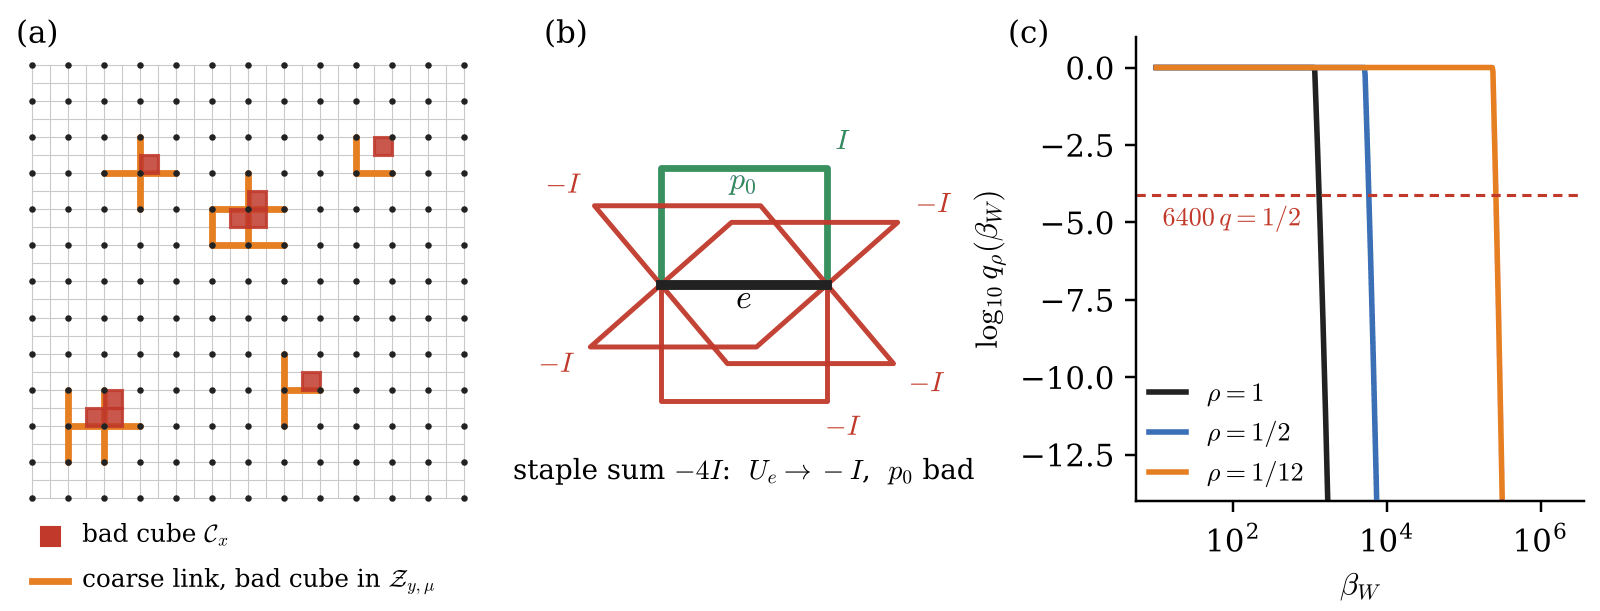
\includegraphics[width=0.95\textwidth]{figures/fig_largefields.png}
\caption{Large fields under the $\SU(2)$ Wilson measure. (a)~A plane section of
the lattice: bad unit cubes (red) form clusters, and the cut-off average can
differ from the path average only on coarse links (orange) whose $24$ cubes
$\mathcal Z_{y,\mu}$ meet a bad cube (Corollary~\ref{cor:activelinks}).
(b)~The frustrated exterior of a link $e$: the staple of $p_0$ is $I$ and the
other five staples are $-I$, so $U_e$ is driven to $-I$ and $p_0$ is bad.
(c)~The weight $q_\rho(\beta_W)$ of Theorem~\ref{thm:defects} for three values
of $\rho$; below the dashed line the cluster bound of
Corollary~\ref{cor:defectclusters} is summable.}
\label{fig:largefields}
\end{figure*}

\begin{corollary}\label{cor:activelinks}
Let $\rho=\frac1{12}$. If no cube of $\mathcal Z_{y,\mu}$ is bad, then
$\chi_{y,\mu}(U)=1$ in the tree gauge, and $V^\sharp_{y,\mu}$ is the average
of the sixteen paths in the chart at $P_{2y}$. A bad cube lies in
$\mathcal Z_{y,\mu}$ for at most eight coarse links, so the expected
fraction of coarse links with $\chi<1$ is at most $4.5\cdot10^5\,(\log
\beta_W+C_0)/\beta_W$. Along the limits of Corollary~\ref{cor:defectclusters},
with probability tending to one these links lie within physical distance
$2a$ of clusters of bad cubes of physical diameter less than any fixed
$R>0$.
\end{corollary}

\begin{proof}
As in the proof of Lemma~\ref{lem:smallstep}, $P_{2y}^{-1}P_x$ is a
product of at most six conjugates of plaquette holonomies or their
inverses. These plaquettes lie in planes $\{\mu,\alpha\}$ with corners
$2y+te_\mu+w$ as above, and a plaquette lies in the unit cube at its
corner. So $\delta(P_x,P_{2y})\le6\rho=\frac12$, and $\chi=1$. A cube with
corner $z$ lies in $\mathcal Z_{y,\mu}$ only if $z_\mu-2y_\mu\in\{0,1,2\}$
and $z_\alpha-2y_\alpha\in\{0,1\}$ for $\alpha\ne\mu$, which leaves at
most two coarse links in each direction. There are $L^4/4$ coarse links,
the number of bad cubes is at most four times the number of bad
plaquettes, and a bad plaquette has $s_p>\rho^2/4$, so by
Lemma~\ref{lem:wilsonZ} the expected fraction is at most $4\cdot8\cdot4
\cdot24\cdot144\,(\log\beta_W+C_0)/\beta_W$. The last assertion is
Corollary~\ref{cor:defectclusters}.
\end{proof}

Small plaquettes everywhere, which Theorem~\ref{thm:smallscales} assumes,
are nevertheless improbable along the one-loop tuning. For $\SU(2)$,
$\beta_W=4g^{-2}$, and the one-loop coupling of
Remark~\ref{rem:constrainedopen}(c) at spacing $a=1/L$ gives $\beta_W=8b_0
\log L+O(1)=\frac{11}{3\pi^2}\log L+O(1)$.

\begin{proposition}\label{prop:manydefects}
Let $0<\rho\le1$, $v_*=\frac2\pi\int_{\arccos(3/4)}^{\pi/3}\sin^2t\,dt$ and
$p=v_*e^{-3\beta_W}$. Conditionally on all other links, a plaquette through
a link $e$ is bad with probability at least $p$. Hence
\[
\mu_L\{\text{no plaquette is bad}\}\le e^{-\lfloor L/3\rfloor^4p},
\]
which tends to $0$ when $\beta_W\le B\log L+O(1)$ with $B<4/3$, in
particular along the one-loop tuning.
\end{proposition}

\begin{proof}
Identify $\SU(2)$ with the unit quaternions. Conditionally on the other
links, $U_e$ has density proportional to $e^{\kappa\,h\cdot u}$ with
$0\le\kappa\le6\beta_W$ and $|h|=1$, the six staples contributing at most
$\beta_W$ each. The plaquette holonomy is $U_e$ or its inverse multiplied
by a fixed element, so it has a density of the same form. Writing the
density as a superposition of indicators of caps centred at $h$, the
probability of a cap about $I$ is largest when $h=I$, and for $h=I$ it
increases with $\kappa$, because its derivative is the covariance of an
increasing function of $\Tr U$ with $\frac12\Tr U$. So the probability of
being bad is at least that of the angle exceeding $\arccos(1-\rho^2/4)\le
\arccos(3/4)$ under the density proportional to $e^{6\beta_W\cos t}\sin^2t$,
which is at least $p$: bound the numerator from below on $[\arccos(3/4),
\pi/3]$, where $\cos t\ge\frac12$, and the denominator by $e^{6\beta_W}
\pi/2$.

Let $M=\lfloor L/3\rfloor$. Choose the links in direction $0$ at the sites
$3z$, $z\in\{0,\dots,M-1\}^4$, and their plaquettes in the plane $\{0,1
\}$. No chosen plaquette contains another chosen link. Removing one chosen
link at a time therefore bounds the probability that all chosen plaquettes
are good by $(1-p)^{M^4}$. With $\beta_W=B\log L+O(1)$ the exponent is of order
$L^{4-3B}$.
\end{proof}

The composition of Theorem~\ref{thm:smallscales} is local, so it continues
across the scales away from the defects, and the defects spread by at most
three spacings of the current scale at each step. For a coarse plaquette $P$
at $y$ let $\mathcal B_P$ be the fine box $2y+[0,4]^4$.

\begin{lemma}\label{lem:localstep}
Let $U$ be a $G$-valued field in the tree gauge and $P$ a coarse plaquette.
If every plaquette $p$ in $\mathcal B_P$ has $\delta(U_p,I)\le\rho_G$ and
$\lVert\Theta_p\rVert\le\eta\le\rho_G/1000$, then $\chi=1$ on the four sides
of $P$, $\delta(V^\sharp(U)_P,I)\le0.03\,\rho_G$, the inequalities
\eqref{eq:smallstep} hold for $P$, and $\lVert\log V^\sharp(U)_P\rVert\le
4(1+647\eta)\eta$.
\end{lemma}

\begin{proof}
For the plaquette $P$ the proof of Lemma~\ref{lem:smallstep} uses only the
plaquettes of the surfaces $\mathcal U_\ell$ of the four sides $\ell$ of $P$
and those of the sixteen squares $\square_{2y+o}$. A plaquette of $\mathcal
U_\ell$, $\ell=(y_i,\mu_i)$, has its corner $x$ at $x_{\mu_i}-2(y_i)_{\mu_i}
\in\{0,1,2\}$ and $x_\alpha-2(y_i)_\alpha\in\{0,1\}$ for $\alpha\ne\mu_i$,
with $y_i\in\{y,y+e_\mu,y+e_\nu\}$; a plaquette of $\square_{2y+o}$ has
$x-2y\in\{0,1,2\}^4$. So $x-2y\in\{0,1,2,3\}^4$ in every case, and the
plaquette lies in $\mathcal B_P$. The bounds on $\chi$, on $\delta(V^\sharp_P,
I)$, the inequalities~\eqref{eq:smallstep} and the bound $\lVert\bar F_P
\rVert+3.2\,r_P^2\le4(1+647\eta)\eta$ in that proof use only the norms of
these plaquettes.
\end{proof}

Let $a$ be the fine spacing and $a_j=2^ja$. Given $\eta_0>0$ put $\eta_{j+1}=
4(1+647\eta_j)\eta_j$. Let $\mathfrak B_0$ be the set of fine plaquettes with
$\delta(U_p,I)>\rho_G$ or $\lVert\Theta_p\rVert>\eta_0$, and let $\mathfrak
B_{j+1}$ be the set of plaquettes $P$ of the lattice of spacing $a_{j+1}$
whose box $\mathcal B_P$ contains a plaquette of $\mathfrak B_j$. Let
$E^\circ_j$ and $A^\circ_j$ be the sum of squares and the sum of $\lVert
\Theta^{(j)}_P\rVert$ over the plaquettes $P\notin\mathfrak B_j$ of the
$j$-th iterate.

\begin{theorem}\label{thm:defectscales}
Let $G\subset\U(r)$ be compact and $U$ a $G$-valued field on the periodic
lattice of side divisible by $2^k$, and suppose that $\eta_j\le\rho_G/1000$
for $j<k$.
\begin{enumerate}[label=\textup{(\roman*)},leftmargin=*]
\item For $j\le k$, every plaquette $P\notin\mathfrak B_j$ of the $j$-th
iterate has $\delta(U^{(j)}_P,I)\le\rho_G$ and $\lVert\Theta^{(j)}_P\rVert
\le\eta_j$. For $j<k$ the cut-off is inactive on the sides of every
plaquette outside $\mathfrak B_{j+1}$, and~\eqref{eq:smallstep} holds
there.
\item Every point of a plaquette of $\mathfrak B_j$ lies within $\ell^\infty$
distance $3(a_j-a)$ of a plaquette of $\mathfrak B_0$.
\item With $\sigma=\sum_{j<k}\eta_j$,
\[
E^\circ_k\le e^{12060\sigma}E^\circ_0,\qquad A^\circ_k\le e^{9147
\sigma}4^{-k}A^\circ_0 .
\]
\item If $4^k\eta_0\le10^{-4}\rho_G$, the hypothesis holds, $\eta_j\le1.023
\cdot4^j\eta_0$ for $j\le k$, $\sigma\le0.35\cdot4^k\eta_0$, and
$E^\circ_k\le1.53\,E^\circ_0$.
\end{enumerate}
\end{theorem}

\begin{proof}
(i) By induction on $j$. If $P\notin\mathfrak B_{j+1}$, no plaquette of
$\mathcal B_P$ lies in $\mathfrak B_j$, so by the induction hypothesis all of
them have $\delta\le\rho_G$ and norm at most $\eta_j\le\rho_G/1000$.
Lemma~\ref{lem:localstep}, applied to the $j$-th iterate in the tree gauge,
gives $\delta(U^{(j+1)}_P,I)\le0.03\,\rho_G$ and $\lVert\Theta^{(j+1)}_P
\rVert\le\eta_{j+1}$; the gauge fixing between steps does not change these
norms.

(ii) Let $P$ at $y$ lie in $\mathfrak B_{j+1}$, and let $p\in\mathfrak B_j$
lie in $\mathcal B_P$, with corner $x$, $x-2y\in\{0,1,2,3\}^4$. In units of
$a_j$ every coordinate of a point of $P$ lies in $[2y_c,2y_c+2]$, and $p$
contains a point whose coordinates are $x_c$ or lie in $[x_c,x_c+1]$; so the
two are at distance at most $3$ in each coordinate. Hence every point of a
plaquette of $\mathfrak B_{j+1}$ is within $3a_j$ of a plaquette of
$\mathfrak B_j$, and $\sum_{i<j}3a_i=3(a_j-a)$.

(iii) Repeat the part \emph{Sums} of the proof of Lemma~\ref{lem:smallstep}
with the plaquettes $P\notin\mathfrak B_{j+1}$ only. Their squares
$\square_{2y+o}$ and surfaces $\mathcal U_\ell$ consist of plaquettes outside
$\mathfrak B_j$, so the same counts give $\sqrt{E^\circ_{j+1}}\le(1+6030
\eta_j)\sqrt{E^\circ_j}$ and $A^\circ_{j+1}\le(1+9147\eta_j)A^\circ_j/4$,
and $1+t\le e^t$.

(iv) The recursion gives $\eta_j\le e^{647\sigma_j}4^j\eta_0$ with $\sigma_j=
\sum_{i<j}\eta_i$. Suppose $\sigma_j\le0.35\cdot4^j\eta_0$, which holds at
$j=0$. Then $\sigma_j\le3.5\cdot10^{-5}$, $e^{647\sigma_j}\le1.023$,
$\eta_j\le1.023\cdot4^j\eta_0\le1.023\cdot10^{-4}\rho_G$, and $\sigma_{j+1}
\le1.373\cdot4^j\eta_0\le0.35\cdot4^{j+1}\eta_0$. Finally $e^{12060\cdot
3.5\cdot10^{-5}}\le1.53$.
\end{proof}

Under the Wilson measure the defects of Theorem~\ref{thm:defectscales} are
the bad plaquettes of Theorem~\ref{thm:defects}. For $\SU(2)$, $\rho_G=1$;
a plaquette with $\delta(U_p,I)=2\sqrt2\sin(\theta/2)\le\rho\le\frac1{10}$
has $\lVert\Theta_p\rVert=\sqrt2\,\theta\le1.01\,\delta(U_p,I)$, so with
$\eta_0=1.01\rho$ every plaquette of $\mathfrak B_0$ is bad, and lies in a
bad cube.

\begin{corollary}\label{cor:defectscales}
Let $G=\SU(2)$, $C_1=C_0+\frac16\log12800$, and for $\beta_W\ge1$ let
$\rho(\beta_W)$ be given by $\rho^2=96(\log\beta_W+C_1)/\beta_W$, so that
$6400\,q_\rho(\beta_W)=\frac12$. Let $k_*$ be the largest integer with
$4^{k_*}\cdot1.01\rho\le10^{-4}$. If $1.01\rho\le10^{-4}$, then $k_*\ge0$,
\[
a_{k_*}\ge1.5\cdot10^{-3}\Bigl(\frac{\beta_W}{\log\beta_W+C_1}\Bigr)^{1/4}a,
\]
and with $\mu_L$-probability at least $1-L^42^{-r}$ every connected cluster
of bad cubes has fewer than $r$ cubes, while for every $j\le k_*$ the
defects of the $j$-th iterate lie within $\ell^\infty$ distance $3a_j$ of
these clusters and the iterate satisfies Theorem~\ref{thm:defectscales}(i),
(iii) with $E^\circ_{k_*}\le1.53\,E^\circ_0$. Along the limits of
Corollary~\ref{cor:defectclusters} with $a\,\rho(\beta_W)^{-1/2}\to0$, which
holds along the one-loop tuning, the defects of all iterates up to the
spacing $a_{k_*}$ lie, with probability tending to one, within clusters of
physical size tending to $0$.
\end{corollary}

\begin{proof}
With this $\rho$, $q_\rho(\beta_W)=\exp(-\log12800)$, and
Corollary~\ref{cor:defectclusters} gives the probability of a connected set
of $r$ bad cubes at most $L^4(6400q)^r=L^42^{-r}$. By maximality, $4^{k_*+1}
\cdot1.01\rho>10^{-4}$, so $2^{k_*}>\frac12\cdot10^{-2}(1.01\rho)^{-1/2}$,
and $\rho^{-1/2}=96^{-1/4}(\beta_W/(\log\beta_W+C_1))^{1/4}$ with $96^{1/4}
<3.14$. The rest is Theorem~\ref{thm:defectscales} with $\eta_0=1.01\rho$,
whose hypothesis holds by part (iv), and $\mathfrak B_0$ contained in the bad
cubes; the bound $\lVert\Theta_p\rVert\le1.01\,\delta(U_p,I)$ applies since
$\rho\le\frac1{10}$. For the limits take $r=\lceil8\log_2L\rceil$, so that
$L^42^{-r}\le L^{-4}$ and $ra\to0$ for a torus of fixed physical side $La$.
The defects then lie in sets of physical diameter at most $ra+6a_{k_*}$, and
$a_{k_*}\le10^{-2}(1.01\rho)^{-1/2}a\to0$.
\end{proof}

The scale $a_{k_*}$ is of the order $(\beta_W/\log\beta_W)^{1/4}a$, the
order of the cube side that the condition (D) needs by
Proposition~\ref{prop:cubesizeN}. So the cut-off average carries the field
through the defects of the Wilson measure, without spreading them, up to
the scale at which (D) can first hold, but not beyond: past $a_{k_*}$ the
bound $\eta_j\le1.023\cdot4^j\eta_0$ no longer keeps the curvature small.
Along the one-loop tuning $\beta_W$ grows like $\log L$, so $k_*$ grows like
$\frac14\log_2\log L$, a vanishing fraction of the $\log_2L$ scales.

The joint bound of Theorem~\ref{thm:defects} is not a conditional one,
and (D) needs a supremum over boundary conditions. The two differ
genuinely. Fix a link $e$ and a plaquette $p_0$ through it. Put all
links on the six staples of $e$ at $I$, except the middle links of the
five staples other than that of $p_0$, which are $-I$. Then the
conditional density of $U_e$ is proportional to $e^{-2\beta_W\Tr U_e}$,
and $p_0$, whose holonomy is $U_e^{\pm1}$, is bad with conditional
probability tending to $1$ as $\beta_W\to\infty$, for every $\rho<2
\sqrt2$. Nearby exteriors behave the same way. So the clusters of
Corollary~\ref{cor:defectclusters} are small in probability, but the
boundary response of a cube to a frustrated exterior is not small, and the
composition beyond the scale $a_{k_*}$ of Corollary~\ref{cor:defectscales}
and the conditional estimate in (D) remain open.

For exteriors that are calm on the boundary of a box and lie in a maximal
torus, the conditional estimate does hold. Let $R=[0,l]^4$, $l\ge2$, be a
box of $\Lambda_L$ with $l<L$. Its boundary $\partial R$ is a cubical
$3$-sphere. Call a link or plaquette of $R$ a \emph{boundary} link or
plaquette if it lies in $\partial R$, and \emph{inner} otherwise. A
plaquette that contains an inner link lies in $R$, so conditionally on all
other links the inner links have the law
\[
\nu_\eta(dU)=Z_\eta^{-1}\exp\Bigl(-\beta_W\sum_{p\in P^\circ}s_p\Bigr)
\prod_edU_e ,
\]
the product over the inner links, where $P^\circ$ is the set of inner
plaquettes. It depends on the exterior $\eta$ only through the boundary
links. Let $T\subset\SU(2)$ be the diagonal torus of the elements
$\exp(tJ)$, $J=\mathrm{diag}(i,-i)$, and for $u\in\SU(2)$ let $\angle u\in
[0,\pi]$ be its angle, so that $\delta(u,I)=2\sqrt2\sin(\angle u/2)$.

\begin{lemma}\label{lem:boxextension}
Let $0\le\rho_s<\pi/3$. Suppose the boundary links of $R$ lie in $T$ and
$\angle U_p\le\rho_s$ for every boundary plaquette. Then the inner links
can be chosen in $T$ so that $\angle U_p\le C\rho_s$ for every plaquette of
$R$, where
\[
C=\sqrt3\,(24\cdot13118+9)<5.46\cdot10^5 .
\]
\end{lemma}

\begin{proof}
Write a $T$-valued field as $U_e=\exp(a_eJ)$ with $a_e\in\R/2\pi\Z$. For a
plaquette $p$ let $(da)_p$ be the signed sum of $a$ over its four links, so
that $U_p=\exp((da)_pJ)$. For a boundary plaquette let $\theta_p\in(-\pi,
\pi]$ be the representative of $(da)_p$; then $|\theta_p|=\angle U_p\le
\rho_s$.

\emph{Closedness.} The signed angles of the six plaquettes of a unit
$3$-cube of $\partial R$ add up to $0$ modulo $2\pi$, since each link occurs
twice with opposite signs. Their representatives add up to a number of
modulus at most $6\rho_s<2\pi$, hence to $0$. So $\theta$ is a closed real
$2$-cochain on $\partial R$.

\emph{Lift.} We construct a real $1$-cochain $\alpha$ on the boundary links
with $d\alpha=\theta$ and $|\alpha_e|\le13118\,l\rho_s$. The boundary is the
union of the eight facets $F_i^0=\{x\in R:x_i=0\}$ and $F_i^l=\{x\in R:x_i=
l\}$, each a cube $[0,l]^3$. Take them in the order $F_1^l$, $F_2^l$,
$F_2^0$, $F_3^l$, $F_3^0$, $F_4^l$, $F_4^0$, $F_1^0$, and let $\Gamma_k$ be
the union of the intersections of the $k$-th facet with the earlier ones.
In the cube of the $k$-th facet, $\Gamma_k$ is empty for $k=1$, one face for
$k=2,3$, three faces, two of them opposite, for $k=4,5$, five faces for
$k=6,7$ and all six for $k=8$. So $\Gamma_k$ is contractible or a
$2$-sphere, and its first cellular cohomology vanishes.

On a facet with coordinates $t_1,t_2,t_3$, the axial gauge gives
$\alpha^0$ with $d\alpha^0=\theta$ on the facet. Put $\alpha^0=0$ on the
links in direction $t_3$. Determine $\alpha^0$ on the links in direction
$t_2$ from the plaquettes in the planes $\{t_2,t_3\}$, starting from $0$ at
$t_3=0$. On the links in direction $t_1$ at $t_3=0$, determine it from the
plaquettes in the plane $\{t_1,t_2\}$, starting from $0$ at $t_2=0$, and
then from the plaquettes in the planes $\{t_1,t_3\}$. The plaquettes in the
planes $\{t_1,t_2\}$ with $t_3>0$ then satisfy $d\alpha^0=\theta$ by
closedness, by induction on $t_3$. Each value is a signed sum of at most
$l$, respectively $2l$, angles, so $|\alpha^0|\le2l\rho_s$.

For $k=1$ put $\alpha=\alpha^0$, so $M_1=\max|\alpha|\le2l\rho_s$. For
$k\ge2$, $\alpha$ is already defined on the links of $\Gamma_k$, with
$|\alpha|\le M_{k-1}$, and $\omega=\alpha-\alpha^0$ is closed there.
Hence $\omega=d\lambda$ for a function $\lambda$ on the vertices of
$\Gamma_k$, and $|\lambda(x)-\lambda(y)|\le\lVert\omega\rVert_\infty
d_\Gamma(x,y)$, where $d_\Gamma$ is the path metric of $\Gamma_k$.

We claim $d_\Gamma\le3d_1$, where $d_1$ is the $\ell^1$ metric of the
facet. If $x$ and $y$ lie in one face of $\Gamma_k$, that face contains an
$\ell^1$ geodesic between them. If they lie in adjacent faces $\{t_i=s\}$
and $\{t_j=s'\}$, the path through the point with $t_i=s$, $t_j=s'$ and
third coordinate that of $x$ has length $d_1(x,y)$. If they lie in opposite
faces $\{t_i=0\}$ and $\{t_i=l\}$, then $d_1(x,y)\ge l$. In that case
$\Gamma_k$ contains a face adjacent to both, and the path from $x$ to that
face, across it and on to $y$ has length at most $d_1(x,y)+2l\le3d_1(x,y)$.

So $\lambda$ is $3\lVert\omega\rVert_\infty$-Lipschitz for $d_1$ on
$\Gamma_k$. The function
\[
\tilde\lambda(x)=\min_y\bigl(\lambda(y)+3\lVert\omega\rVert_\infty d_1(x,y)
\bigr)
\]
extends it to the vertices of the facet with the same constant~\cite{McS34}.
Put $\alpha=\alpha^0+d\tilde\lambda$ on the links of the facet. It agrees
with the earlier values on $\Gamma_k$, satisfies $d\alpha=\theta$ on the
facet, and has
\[
|\alpha|\le2l\rho_s+3(M_{k-1}+2l\rho_s).
\]
So $M_k\le3M_{k-1}+8l\rho_s$, which gives $M_8\le13118\,l\rho_s$.

\emph{Extension.} Let $c$ be the centre of $R$, $R_0=l/2$, $r(x)=|x-c|_\infty$
and $\varphi(x)=c+R_0(x-c)/r(x)$, the radial projection of $R\setminus\{c\}$
onto $\partial R$. Let $\hat\alpha$ and $\hat\theta=d\hat\alpha$ be the
lowest-order Whitney forms of $\alpha$ and $\theta$ on the unit cubes of
$\partial R$~\cite{Whi57}. On a unit cube with coordinates $t_1,t_2,t_3$,
$\hat\alpha=\sum_ia_i\,dt_i$, where $a_i$ is the multilinear interpolation of
the values of $\alpha$ on the four links in direction $t_i$; similarly
$\hat\theta=\sum_{i<j}\theta_{ij}\,dt_i\wedge dt_j$. These forms have
continuous tangential components across the faces of the unit cubes, satisfy
$\int_e\hat\alpha=\alpha_e$ for every boundary link, and for tangent
vectors
\[
|\hat\alpha(u)|\le\sqrt3\,M_8|u|,\qquad|\hat\theta(u,w)|\le\sqrt3\,\rho_s
|u||w| .
\]
Put $\tilde B=(r/R_0)^2\varphi^*\hat\alpha$ on $R\setminus\{c\}$. Since
$|\nabla r|=1$ almost everywhere and $|x-c|\le2r$, we have $|d\varphi(v)|\le
3R_0|v|/r$. Then
\[
d\tilde B=d\bigl(r^2/R_0^2\bigr)\wedge\varphi^*\hat\alpha+(r/R_0)^2
\varphi^*\hat\theta
\]
gives
\[
|d\tilde B(v,w)|\le\bigl(12\sqrt3\,M_8/R_0+9\sqrt3\,\rho_s\bigr)|v||w|\le
C\rho_s|v||w| ,
\]
and $|\tilde B|\le3\sqrt3\,M_8r/R_0$ is bounded.

The set $R\setminus\{c\}$ is the union of the cones from $c$ over the unit
cubes of $\partial R$. These cones are convex polytopes cut out by
hyperplanes through $c$. On each of them $\tilde B$ is smooth, and its
tangential components are continuous across them since $\varphi$ is
continuous. Put $B_e=\int_e\tilde B$ for every link $e$ of $R$. Apply
Stokes' theorem on each piece of a plaquette: the boundary terms on the
interior cuts cancel, and the point $c$ contributes nothing since $\tilde B$
is bounded. This gives $(dB)_p=\int_pd\tilde B$, so $|(dB)_p|\le C\rho_s$.
On $\partial R$, $r=R_0$ and $\varphi$ is the identity on tangent vectors,
so $B=\alpha$ on the boundary links.

\emph{Gauge.} The cochain $a-\alpha$ on the boundary links has
$(d(a-\alpha))_p\equiv\theta_p-\theta_p=0$ modulo $2\pi$ on every boundary
plaquette. So it is a flat $\U(1)$-field on the $2$-skeleton of $\partial
R$, which is simply connected, and $a-\alpha\equiv d\mu$ modulo $2\pi$ for a
function $\mu$ on the boundary vertices. Extend $\mu$ by $0$ to the inner
vertices and put $U_e=\exp((B_e+(d\mu)_e)J)$ on the inner links. On the
boundary links $B+d\mu\equiv a$, and every plaquette of $R$ has angle at
most $|(dB)_p|\le C\rho_s$.
\end{proof}

For a general $\SU(2)$-valued boundary field the curvature is not a closed
cochain, and the lift in the proof of Lemma~\ref{lem:boxextension} is not
available. A lift by gluing local gauges still works when $l^2\rho_s$ is
small. Identify $\mathfrak{su}(2)$ with the imaginary quaternions and write
$|X|$ for the operator norm, which is the Euclidean norm, so that
$|[X,Y]|\le2|X||Y|$, $\lVert e^X-I\rVert\le|X|$ and $\angle e^X=|X|$ for
$|X|\le\pi$. With $d(g,h)=\angle(g^{-1}h)$, the map $X\mapsto e^X$ is
$1$-Lipschitz, since its differential has singular values $1$ and
$\sin|X|/|X|$, and the principal logarithm is $2$-Lipschitz on $\{\angle
h\le\frac12\}$, a geodesically convex ball on which the inverse
differential has singular values at most $\frac12/\sin\frac12<2$. Put
\[
C_1=2,\qquad C_k=11\,C_{k-1}+24\quad(2\le k\le8),
\]
so that $C_8=85\,743\,550$, and
\[
K=42\,C_8+20,\qquad \varepsilon_0=\frac1{100\,C_8^2}.
\]

\begin{lemma}\label{lem:nonabelianfilling}
Let the boundary links $\eta$ of $R$ take values in $\SU(2)$, with
$\angle\eta_p\le\rho_s$ for every boundary plaquette and $l^2\rho_s\le
\varepsilon_0$. Then the inner links can be chosen so that $\angle U_p\le
K\rho_s$ for every plaquette of $R$.
\end{lemma}

\begin{proof}
For a vertex gauge $g$ write $\eta^g_{xy}=g_x\eta_{xy}g_y^{-1}$. A product
of conjugates of $m$ elements of angle at most $\rho_s$ has angle at most
$m\rho_s$, since $d$ is bi-invariant.

\emph{One facet.} On a facet with coordinates $t_1,t_2,t_3$ let $P_x$ be
the path from the corner to $x$ that moves first in direction $t_1$, then
$t_2$, then $t_3$, and put $g^0_x=\eta(P_x)$, the ordered product of the links along
$P_x$. Then $\eta^{g^0}_{xy}$ is the holonomy of the loop $P_x\,(xy)\,
P_y^{-1}$. For a link in
direction $t_3$ this loop retraces itself. For a link in direction $t_2$ at
height $t_3=c$ it bounds $c$ plaquettes of the planes $\{t_2,t_3\}$, and
for a link in direction $t_1$ at $(t_2,t_3)=(b,c)$ it bounds $b$
plaquettes of a plane $\{t_1,t_2\}$ and $c$ of a plane $\{t_1,t_3\}$. So
the holonomy is a product of conjugates of at most $2l$ plaquette
holonomies, and every link of the facet has $\angle\eta^{g^0}_e\le
2l\rho_s$.

\emph{Gluing.} Take the facets in the order of the proof of
Lemma~\ref{lem:boxextension}, with the same sets $\Gamma_k$; there
$d_\Gamma\le3d_1$. Two vertices of $\Gamma_k$ joined by a link of the
facet lie in a common face of $\Gamma_k$, since $l\ge2$, so that link
lies in $\Gamma_k$. We construct a gauge $g$ on the boundary vertices with
$\angle\eta^g_e\le M_k=C_kl\rho_s$ on the links of the first $k$ facets.
For $k=1$ take $g=g^0$. For $k\ge2$, let $g^0$ be the gauge of the $k$-th
facet and $t_x=g_x(g^0_x)^{-1}$ for $x\in\Gamma_k$. For a link $xy$ of
$\Gamma_k$, $\eta^g_{xy}=t_x\eta^{g^0}_{xy}t_y^{-1}$, so
\[
d(t_x,t_y)=\angle\bigl(t_x^{-1}t_y\bigr)\le\angle\eta^g_{xy}+\angle
\eta^{g^0}_{xy}\le M_{k-1}+2l\rho_s ,
\]
and $t$ is $3(M_{k-1}+2l\rho_s)$-Lipschitz for $d_1$ on $\Gamma_k$. Fix
$x_0\in\Gamma_k$ and put $h_x=t_{x_0}^{-1}t_x$. The facet has $d_1$-diameter
$3l$, so
\[
\angle h_x\le9l(M_{k-1}+2l\rho_s)=9(C_{k-1}+2)\,l^2\rho_s\le9(C_8+2)
\varepsilon_0<\tfrac12 ,
\]
and $a_x=\log h_x$ is $L$-Lipschitz for $d_1$, with
$L=6(M_{k-1}+2l\rho_s)$. Extend each of the three real coordinates of $a$
to the vertices of the facet by the formula of McShane~\cite{McS34}, as in
the proof of Lemma~\ref{lem:boxextension}; the extension $\tilde a$ is
$\sqrt3L$-Lipschitz. Put $g_x=t_{x_0}e^{\tilde a_x}g^0_x$ on the facet; on
$\Gamma_k$ this is the old value. For a link $xy$ of the facet,
$\eta^g_{xy}=\tilde t_x\eta^{g^0}_{xy}\tilde t_y^{-1}$ with $\tilde t_x=
t_{x_0}e^{\tilde a_x}$, so
\[
\begin{split}
\angle\eta^g_{xy}&\le d(\tilde t_x,\tilde t_y)+2l\rho_s\le\sqrt3L+2l\rho_s\\
&=6\sqrt3\,M_{k-1}+(12\sqrt3+2)\,l\rho_s\le M_k .
\end{split}
\]
After the eighth facet, $\angle\eta^g_e\le M=C_8l\rho_s$ on every boundary
link.

\emph{Potential.} Since $M\le C_8\varepsilon_0/l<\frac12$, the logarithms
$A_e=\log\eta^g_e$ are defined, with $|A_e|\le M$ and $A_{-e}=-A_e$. Let
$(dA)_p$ be the signed sum of $A$ over the four links of a boundary
plaquette. For $X_1,\dots,X_q\in\mathfrak{su}(2)$,
\[
\Bigl\lVert e^{X_1}\cdots e^{X_q}-I-\sum_iX_i\Bigr\rVert\le\tfrac12\Bigl(
\sum_i|X_i|\Bigr)^2 ,
\]
by induction on $q$ from $e^Xe^Y-I-X-Y=(e^X-I-X)+(e^Y-I-Y)+(e^X-I)(e^Y-I)$
and $\lVert e^X-I-X\rVert\le|X|^2/2$. Applied to the four links of $p$, and
since $\lVert\eta^g_p-I\rVert=2\sin(\angle\eta_p/2)\le\rho_s$, this gives
\[
|(dA)_p|\le\sigma=\rho_s+8M^2 .
\]
Let $\hat A$ be the lowest-order Whitney form of $A$ on the unit cubes of
$\partial R$, as in the proof of Lemma~\ref{lem:boxextension}, now with
values in $\mathfrak{su}(2)$. Its coefficients are interpolations of values
of $A$, and those of $d\hat A$ are interpolations of values of $dA$, so
\[
|\hat A(u)|\le\sqrt3\,M|u|,\qquad|d\hat A(u,w)|\le\sqrt3\,\sigma|u||w| .
\]
With $r$, $R_0$ and $\varphi$ as there, put $\tilde B=(r/R_0)^2\varphi^*
\hat A$ on $R\setminus\{c\}$ and $\tilde B(c)=0$. The same computation
gives
\[
|\tilde B(v)|\le3\sqrt3\,M\frac r{R_0}|v|,\qquad|d\tilde B(v,w)|\le\kappa_1
|v||w|,
\]
where $\kappa_1=12\sqrt3\,M/R_0+9\sqrt3\,\sigma$.
On each cone from $c$ over a unit cube of $\partial R$, $\tilde B$ is
smooth away from $c$, and its tangential components are continuous across
the cones.

\emph{Transport.} For a link $e$ of $R$, parametrised by $s\in[0,1]$, let
$V_e=T(1)$, where $T'=T\,\tilde B(\dot e)$ and $T(0)=I$; the coefficient is
bounded and piecewise smooth, and $V$ composes along paths in the order of
the links. For a closed path $\gamma$ of length $\ell$,
\[
T(1)-I-\int_\gamma\tilde B=\int_0^1(T-I)\,\tilde B(\dot\gamma)\,ds,
\]
and $\lVert T(s)-I\rVert\le\int_0^s|\tilde B(\dot\gamma)|$,
so the holonomy $V_\gamma$ satisfies $\lVert V_\gamma-I\rVert\le|\int_\gamma
\tilde B|+\frac12(\int_\gamma|\tilde B|)^2$. Let $p$ be a plaquette of $R$
and divide it into $N^2$ squares $q$ of side $h=1/N$. Its holonomy is a
product of conjugates of the holonomies of the boundaries of the squares,
since every inner edge of the subdivision is traversed once in each
direction. For each square, Stokes' theorem on the finitely many convex
polygons in which the cones cut $q$ gives $\int_{\partial q}\tilde B=
\int_qd\tilde B$: the integrals over the interior cuts cancel because the
tangential components agree, and if $c\in q$ a disc of radius $\delta$
around $c$ contributes $O(\delta^2)$, since $|\tilde B|\le3\sqrt3\,Mr/R_0$.
Hence
\[
\lVert V_{\partial q}-I\rVert\le\kappa_1h^2+\tfrac12\bigl(4h\cdot3\sqrt3\,M
\bigr)^2=\kappa h^2,
\]
with $\kappa=\kappa_1+216M^2$.
Since $2\arcsin(x/2)\le x(1+x^2)$ for $0\le x\le1$, summing over the
squares gives $\angle V_p\le\kappa(1+\kappa^2N^{-4})$, and letting
$N\to\infty$, $\angle V_p\le\kappa$. Now $M/R_0=2C_8\rho_s$ and
$M^2=C_8^2l^2\rho_s^2\le\rho_s/100$, so
\[
\begin{split}
\kappa&\le\bigl(24\sqrt3\,C_8+9\sqrt3\bigr)\rho_s+\bigl(72\sqrt3+216\bigr)M^2\\
&<(42\,C_8+20)\,\rho_s=K\rho_s .
\end{split}
\]

\emph{Boundary values.} On $\partial R$, $r=R_0$ and $\varphi$ is the
identity on tangent vectors, and along a boundary link $e$ the tangential
coefficient of $\hat A$ is the constant $A_e$. So $V_e=e^{A_e}=\eta^g_e$.
Extend $g$ by $I$ to the inner vertices and put $U_{xy}=g_x^{-1}V_{xy}g_y$.
Then $U=\eta$ on the boundary links, and $U_p$ is conjugate to $V_p$, so
$\angle U_p\le K\rho_s$ for every plaquette of $R$.
\end{proof}

The boundary fields of Lemma~\ref{lem:nonabelianfilling} with strict
inequalities form an open set of positive Haar measure that contains the
identity field; unlike those of Lemma~\ref{lem:boxextension}, they are not
a null set. The constants are far from optimal.

For $0<\varepsilon\le1$ let $E_\varepsilon$ be the event that at least
$\varepsilon l^4$ of the $l^4$ unit cubes $x+[0,1]^4$, $x\in\{0,\dots,
l-1\}^4$, of $R$ contain a bad plaquette.

\begin{proposition}\label{prop:conddensity}
Let $\beta_W\ge1$ and $0<\rho\le1$. Suppose that no boundary plaquette of
$R$ is bad under $\eta$, and that the inner links can be chosen so that
every inner plaquette has angle at most $\kappa$. Then
\[
\begin{split}
-\log\nu_\eta(E_\varepsilon)\ge{}&\frac{\beta_W\rho^2\varepsilon}{16}\,l^4\\
&-6(l+1)^4\bigl(\log\beta_W+C_0+\tfrac12+\beta_W\kappa^2\bigr),
\end{split}
\]
with $C_0$ as in Lemma~\ref{lem:wilsonZ}. In particular, if the boundary
links lie in $T$ with angle at most $\rho_s<\pi/3$ on every boundary
plaquette and $\rho\ge\sqrt2\,\rho_s$, the bound holds with $\kappa=C\rho_s$
and the constant $C$ of Lemma~\ref{lem:boxextension}. If the boundary
links lie in $\SU(2)$ with angle at most $\rho_s$ on every boundary
plaquette, $l^2\rho_s\le\varepsilon_0$ and $\rho\ge\sqrt2\,\rho_s$, it
holds with $\kappa=K\rho_s$.
\end{proposition}

\begin{proof}
On $E_\varepsilon$ the bad plaquettes are inner, and each lies in at most
four of the unit cubes. So there are at least $\varepsilon l^4/4$ of them,
each with $s_p>\rho^2/4$, and $\sum_{P^\circ}s_p\ge\rho^2\varepsilon l^4
/16$. Hence the unnormalised weight of $E_\varepsilon$ is at most $\exp(
-\beta_W\rho^2\varepsilon l^4/16)$.

For the normalisation let $\bar U$ be the inner links of the hypothesis,
$t=(4\sqrt{\beta_W})^{-1}$, and consider the inner links $U_e=\bar U_eh_e$
with $\angle h_e\le t$. The angle of $g^{-1}h$ is a bi-invariant distance,
so every inner plaquette has $\angle U_p\le\kappa+4t$ and
\[
s_p\le\tfrac12(\kappa+4t)^2\le\kappa^2+16t^2=\kappa^2+\beta_W^{-1} .
\]
Each $h_e$ has probability at least $8t^3/(3\pi^3)=(24\pi^3\beta_W^{3/2}
)^{-1}$, as in the proof of Lemma~\ref{lem:wilsonZ}. There are $n_P\le6l^2
(l+1)^2$ inner plaquettes and $n_L\le4l(l+1)^3$ inner links, so
\[
Z_\eta\ge\exp\bigl(-n_P(\beta_W\kappa^2+1)\bigr)\bigl(24\pi^3\beta_W^{3/2}
\bigr)^{-n_L}.
\]
Since $C_0=\frac12+\frac23\log(24\pi^3)$, $n_P+n_L\log(24\pi^3\beta_W^{3/2}
)\le6(l+1)^4(\log\beta_W+C_0+\frac12)$, which gives the bound. For the last
assertion, a boundary plaquette has $\delta(U_p,I)\le\sqrt2\,\angle U_p\le
\sqrt2\,\rho_s\le\rho$, so it is not bad, and Lemma~\ref{lem:boxextension}
or Lemma~\ref{lem:nonabelianfilling} gives the inner links.
\end{proof}

So in a box whose boundary is calm at a level $\rho_s$ small compared with
$\rho\sqrt\varepsilon/C$ and $T$-valued, or small compared with
$\rho\sqrt\varepsilon/K$ and $\SU(2)$-valued with $l^2\rho_s\le
\varepsilon_0$, the fraction of bad cubes
exceeds $\varepsilon$ only with probability exponentially small in the
volume once $\beta_W\rho^2\varepsilon$ is large compared with $\log
\beta_W$, uniformly over such exteriors and over $l$. The estimate is
conditional, unlike Theorem~\ref{thm:defects}.

\begin{remark}\label{rem:boxnonabelian}
The exteriors with boundary links in $T$ form a null set for $\mu_L$.
Lemma~\ref{lem:nonabelianfilling} removes the torus at the price of the
smallness $l^2\rho_s\le\varepsilon_0$. In the continuum the corresponding
condition is that of Uhlenbeck's theorem~\cite{Uhl82}, which gives a
Coulomb gauge on a ball when the curvature is small in $L^{n/2}$; on
$3$-dimensional pieces of $\partial R$ of side comparable to $l$ and for
curvature of size $\rho_s$ this norm is of order $l^2\rho_s$. The lemma
replaces the Coulomb gauge by the gluing of the facet gauges. With
$\rho_s$ of the order of the level $\rho(\beta_W)$ of
Corollary~\ref{cor:defectscales}, $\rho_s=c_0(\log\beta_W/\beta_W)^{1/2}$,
it applies for
\[
l\le(\varepsilon_0/c_0)^{1/2}\,(\beta_W/\log\beta_W)^{1/4},
\]
the scale $a_{k_*}$ of Corollary~\ref{cor:defectscales} up to a constant
factor. Along the tuning $\beta_W\sim b\log(1/a)$ the physical side $al$
then tends to $0$, so the lemma does not reach cubes of a fixed physical
size; this is a limitation of the argument, not a proof that such fillings
fail. Moreover Proposition~\ref{prop:conddensity} bounds the fraction of
bad cubes under one exterior and does not compare the laws under two
exteriors, so it gives no contraction coefficient. The conditional
estimate in (D), for calm exteriors on cubes of fixed physical size, remains
open.
\end{remark}

\section*{Acknowledgements}

This paper rests on the work of many earlier scientists. Lattice gauge
theory is due to Wilson~\cite{Wil74} and its Hamiltonian form to Kogut and
Susskind~\cite{KS75}; reflection positivity and the reconstruction of the
transfer matrix to Osterwalder and Schrader~\cite{OS73,OS75}, and their
lattice form, with the first proof of a gap at strong coupling, to
Osterwalder and Seiler~\cite{OSei78,Sei82}. The uniqueness method is
Dobrushin's~\cite{Dob68,Dob70,DS85}, the curvature method is that of Bakry
and \'Emery~\cite{BE85,BGL14} in the form of Shen, Zhu and Zhu~\cite{SZZ23},
the gauge fixing on a forest is Creutz's~\cite{Cre77}, and the curvature of
Lie groups is Milnor's~\cite{Mil76}; the localisation estimate of
Sec.~\ref{ssec:constrained} is that of Combes and Thomas~\cite{CT73}. The analysis of the single-link law
uses results of Barta~\cite{Bar37}, Biernacki and Krzy\.z~\cite{BK55},
McShane~\cite{McS34}, Stein and Weiss~\cite{SW71} and Watson~\cite{Wat44}, and
the continuum problem is the one formulated by Jaffe and Witten~\cite{JW06}
and studied by Ba{\l}aban~\cite{Bal84a,Bal85a,Bal89b}.

\section*{Data and code availability}

The proofs are analytic except for the evaluations in
Propositions~\ref{prop:cover} and~\ref{prop:cover2} and
Lemma~\ref{lem:su3const} and the numerical bounds of
Lemma~\ref{lem:vmfconst}, which are computations in interval arithmetic with
rigorous error bounds, and for Proposition~\ref{prop:blockgapsharp} and
Theorem~\ref{thm:certificate}, whose certificates are checked in exact
arithmetic. The programs of these steps, in Python with
python-flint (FLINT and Arb) and a C kernel for products of Taylor
polynomials, their outputs and the list of certified boxes are in the
repository \url{https://github.com/creelie/4Y-M}, release v4.20.0, together
with a Lean~4 certificate of the line field, independent exact or
numerical checks of the other finite statements, our checks of the
certificate of~\cite{Rom26}, and the certificate of
Proposition~\ref{prop:blockgapsharp} with its exact check. The code was
written by Deep Bhattacharjee, James Montgomery Lockwood and Tristan
Romanov.

The computations, the checks and parts of the drafting were done with AI
assistance (Claude Opus~5.5,
Claude Fable~5.1, GPT-6.1 Sol Ultra and GPT-6 Astra Ultra) under the
direction of Deep Bhattacharjee. The combination of the forest gauge with
the sharp quarter behind Theorem~\ref{thm:su2} was first assembled by
Anaxia, the reasoning engine of the BLLM system~\cite{Bha26,Bha26b}; the line
field, the free-boundary limit, the ceiling, the curvature bound, the
$\SU(3)$ part, the plaquette blocks and the certified constants are the
authors' own. All four authors
approved the final text.

\section*{Declarations}

\emph{Funding.} None. \emph{Competing interests.} None. \emph{Ethics
approval.} Not applicable: the work involves no human participants, animals
or personal data.

\appendix

\section{The line field}\label{app:table}

Table~\ref{tab:sigma} lists, for each residue class of $x$ modulo two, the
direction $\sigma(x)$ and the permutation $\pi_x(\mu)=\sigma(x+e_\mu)$. In every
row $\pi_x$ fixes $\sigma(x)$ and is a three-cycle on the other directions,
which is the condition of Lemma~\ref{lem:cycle}.

\begin{table}[h]
\caption{The line field: $x$ modulo two (digits $x_0x_1x_2x_3$), the
direction $\sigma(x)$ and the values $\sigma(x+e_\mu)$ for $\mu=0,1,2,3$.}
\label{tab:sigma}
\begin{ruledtabular}
\begin{tabular}{cccccc}
$x$&$\sigma(x)$&$\mu=0$&$\mu=1$&$\mu=2$&$\mu=3$\\
\colrule
0000 & 0 & 0 & 2 & 3 & 1 \\
1000 & 0 & 0 & 3 & 1 & 2 \\
0100 & 2 & 3 & 0 & 2 & 1 \\
1100 & 3 & 2 & 0 & 1 & 3 \\
0010 & 3 & 1 & 2 & 0 & 3 \\
1010 & 1 & 3 & 1 & 0 & 2 \\
0110 & 2 & 1 & 3 & 2 & 0 \\
1110 & 1 & 2 & 1 & 3 & 0 \\
0001 & 1 & 2 & 1 & 3 & 0 \\
1001 & 2 & 1 & 3 & 2 & 0 \\
0101 & 1 & 3 & 1 & 0 & 2 \\
1101 & 3 & 1 & 2 & 0 & 3 \\
0011 & 3 & 2 & 0 & 1 & 3 \\
1011 & 2 & 3 & 0 & 2 & 1 \\
0111 & 0 & 0 & 3 & 1 & 2 \\
1111 & 0 & 0 & 2 & 3 & 1 \\
\end{tabular}
\end{ruledtabular}
\end{table}

\section{The comparison lemma}\label{app:comparison}

Let $(G,\delta)$ be a compact group with a bi-invariant metric of diameter
$D$, $\Omega=G^A$, and $C_{ee'}$ the coefficients of Sec.~\ref{sec:state},
with row and column sums at most $\alpha<1$ and $C_{ee'}=0$ unless $e,e'$ share
a plaquette, so that $|e-e'|\le1$ for the distance of link midpoints. Fix
$\lambda>0$ with $\theta=\alpha e^\lambda<1$.

\begin{lemma}\label{lem:comparison}
Let $S\subset A$, possibly infinite, and let $\mu_1,\mu_2$ be probability
measures on $\Omega$ invariant under $\gamma^F_e$ for every $e\notin S$. Let
$T\subset A\setminus S$ be finite, $w_b=e^{-\lambda\dist(b,T)}$, and suppose
$\sum_{z\in S}w_z<\infty$. There is a coupling of $\mu_1,\mu_2$ whose link
distances $\varrho(b)=\E\,\delta(\sigma_b,\sigma'_b)$ satisfy
\[
\sum_{b\notin S}w_b\varrho(b)\le\frac{\theta D}{1-\theta}\sum_{z\in S}w_z .
\]
If $S=\emptyset$ then $\mu_1=\mu_2$.
\end{lemma}

\begin{proof}
The couplings form a weakly compact set and $\Psi(\pi)=\sum_bw_b\E_\pi\delta(
\sigma_b,\sigma'_b)$ is weakly continuous because $\sum_bw_b<\infty$; let $\pi^*$ be
a minimiser. For $e\notin S$ replace the pair $(\sigma_e,\sigma'_e)$ by a sample of
an optimal coupling of $\gamma^F_e(\cdot\mid\sigma)$ and $\gamma^F_e(\cdot\mid
\sigma')$, chosen measurably~\cite[Cor.~5.22]{Vil09}. Both $\mu_i$ are
invariant, so the result is again a coupling, and changing the finitely
many links that enter $\gamma^F_e$ one at a time gives $W_1\le\sum_{e'}C_{ee'}
\delta(\sigma_{e'},\sigma'_{e'})$. Minimality gives $\varrho(e)\le\sum_{e'}C_{ee'}
\varrho(e')$. Multiply by $w_e$ and sum over $e\notin S$; where $C_{ee'}\ne0$,
$w_e\le e^\lambda w_{e'}$, so
\[
\sum_{e\notin S}w_e\varrho(e)\le\theta\Bigl[\sum_{e'\notin S}w_{e'}\varrho(e')
+\sum_{z\in S}w_z\varrho(z)\Bigr],
\]
all sums are finite, and $\varrho\le D$ on $S$. If $S=\emptyset$, $\varrho\equiv0$.
\end{proof}

\begin{corollary}\label{cor:decay}
Let $\mu$ be the Gibbs measure of $\gamma^F$, $F$ a local function with
support $S_F$, $L_F$-Lipschitz in each link, and $H$ bounded with finite
support $S_H$ disjoint from $S_F$. Then
\[
|\Cov_\mu(F,H)|\le\|H\|_\infty L_F\frac{\theta D}{1-\theta}|S_H|\,
e^{-\lambda\dist(S_F,S_H)}.
\]
\end{corollary}

\begin{proof}
Condition on the links of $S_H$~\cite[Ch.~3]{Kal21}; the conditional
measures $\mu^\sigma=\mu(\cdot\mid\sigma_{S_H})$ are invariant under
$\gamma^F_e$ for $e\notin S_H$. Lemma~\ref{lem:comparison} with $S=S_H$ and
$T=S_F$, for which $w_b=1$ on $S_F$ and $w_z\le e^{-\lambda\dist(S_F,S_H)}$ on
$S_H$, gives
$|\mu^\sigma(F)-\mu^{\sigma'}(F)|\le L_F\sum_{b\in S_F}\varrho(b)\le
L_F\frac{\theta D}{1-\theta}|S_H|e^{-\lambda\dist(S_F,S_H)}$ for any two
boundary values. Since $H$ depends only on $\sigma_{S_H}$,
$\Cov_\mu(F,H)=\iint H(\sigma)\bigl(\mu^\sigma(F)-\mu^{\sigma'}(F)\bigr)\,
d\mu(\sigma)\,d\mu(\sigma')$, and the bound follows.
\end{proof}

\begin{lemma}\label{lem:blockcomparison}
Let the blocks partition $A$, let $C_{Bj}$ be the block coefficients of
Sec.~\ref{sec:plaqblocks}, with $\sum_BC_{Bj}\le\alpha<1$ for every $j$ and
$C_{Bj}=0$ unless every link of $B$ lies within distance $2$ of $j$, and fix
$\lambda>0$ with $\theta=\alpha e^{2\lambda}<1$. Let $S\subset A$ be a union
of blocks and let $\mu_1,\mu_2$ be invariant under $\gamma^{\mathcal B}_B$ for
every block $B\not\subset S$. With $T$, $w_b$ as in
Lemma~\ref{lem:comparison} and $\sum_{z\in S}w_z<\infty$, there is a coupling
with $\sum_{b\notin S}w_b\varrho(b)\le\frac{\theta D}{1-\theta}\sum_{z\in S}w_z$,
and $\mu_1=\mu_2$ if $S=\emptyset$.
\end{lemma}

\begin{proof}
Take a minimiser $\pi^*$ of $\Psi$ as before. For a block $B\not\subset S$
replace $(\sigma_B,\sigma'_B)$ by an optimal coupling, for the metric $d$, of
the two block laws; it is again a coupling, and changing the boundary links
one at a time bounds the expected new $d$-distance by $\sum_jC_{Bj}\varrho(j)$.
Put $\bar w_B=\max_{i\in B}w_i$. Minimality gives
\[
\sum_{i\in B}w_i\varrho(i)\le\bar w_B\sum_jC_{Bj}\varrho(j),
\]
and $\bar w_B\le e^{2\lambda}w_j$ whenever $C_{Bj}\ne0$. Summing over the
blocks outside $S$ and using the column sums,
\[
\sum_{b\notin S}w_b\varrho(b)\le\theta\Bigl[\sum_{j\notin S}w_j\varrho(j)+
\sum_{z\in S}w_z\varrho(z)\Bigr],
\]
which gives the claim as in Lemma~\ref{lem:comparison}.
\end{proof}

\begin{lemma}\label{lem:dscomparison}
Let $n\ge2$ be even, let $V_x$, $x\in2\Z^4$, be the translates of
Sec.~\ref{sec:bypass}, and suppose that $D(n,\alpha)$ holds.
\begin{enumerate}[label=\textup{(\alph*)},leftmargin=*]
\item If a probability measure $\mu$ on $G^A$ is invariant under
$\gamma^F_e$ for every $e$ in a finite set $V$, it is invariant under
$\gamma_V$.
\item Fix $\lambda>0$ with $\theta=\alpha e^{\lambda\rho_n}<1$. Let $S\subset
A$, and let $\mu_1,\mu_2$ be invariant under $\gamma_{V_x}$ for every $x$
with $V_x\cap S=\emptyset$. With $T$, $w_b$ as in Lemma~\ref{lem:comparison}
and $\sum_{z\in S}w_z<\infty$, there is a coupling with
\[
\sum_{b\notin S}w_b\varrho(b)\le\frac{D(1+c_ne^{\lambda\rho_n})}{1-\theta}
\sum_{z\in S}w_z ,
\]
and $\mu_1=\mu_2$ if $S=\emptyset$.
\end{enumerate}
\end{lemma}

\begin{proof}
(a) Let $\nu_\eta$ be the conditional law of $Q_V$ given the links $\eta$
outside $V$. For bounded $f$ on $G^V$ and bounded $g$ of $\eta$,
$\gamma^F_e(fg)=g\,\gamma^F_ef$ for $e\in V$, so invariance gives $\int
g(\eta)\bigl(\nu_\eta(\gamma^F_ef)-\nu_\eta(f)\bigr)\,d\mu=0$ for all $g$;
taking $f$ in a countable dense set of continuous functions, $\nu_\eta$ is
invariant under every $\gamma^F_e(\cdot\mid\cdot,\eta)$, $e\in V$, for
$\mu$-almost every $\eta$. So is $\gamma_V(\cdot\mid\eta)$, whose
conditional laws of single links are the $\gamma^F_e$. The composition $P_\eta$
of the kernels $\gamma^F_e$, $e\in V$, in a fixed order has a density with
respect to Haar measure on $G^V$ bounded below by a positive constant,
because each single-link density is at least $e^{-12N^2\beta}$ times its
maximum over the group. A Markov kernel with such a lower bound has at most
one invariant probability measure (Doeblin's condition), so
$\nu_\eta=\gamma_V(\cdot\mid\eta)$.

(b) Let $\pi^*$ minimise $\Psi$ as in Lemma~\ref{lem:comparison} and call $x$
admissible if $V_x\cap S=\emptyset$. For admissible $x$ replace
$(\sigma_{V_x},\sigma'_{V_x})$ by an optimal coupling, for $d_{V_x}$, of the
two block laws; both $\mu_i$ are invariant, so the result is a coupling, and
changing the boundary links one at a time bounds the new expected
$d_{V_x}$-distance by $\sum_jC_{V_x,j}\varrho(j)$. With $\bar w_x=\max_{i\in
V_x}w_i$, minimality gives
\[
\sum_{i\in V_x}w_i\varrho(i)\le\bar w_x\sum_{j\notin V_x}C_{V_x,j}\varrho(j),
\]
and $\bar w_x\le e^{\lambda\rho_n}w_j$ whenever $C_{V_x,j}\ne0$. Let $S'$ be
the set of links outside $S$ that lie in a translate meeting $S$; each is
within distance $\rho_n$ of a link of $S$, so $\sum_{i\in S'}w_i\le
c_ne^{\lambda\rho_n}\sum_{z\in S}w_z$. A link outside $S\cup S'$ lies in
$N_n$ translates, all admissible. Summing over admissible $x$ and using
$\sum_{x:\,j\notin V_x}C_{V_x,j}=K_{c(j)}\le\alpha N_n$,
\[
N_n\sum_{i\notin S\cup S'}w_i\varrho(i)\le\theta N_n\Bigl[\sum_{i\notin
S\cup S'}w_i\varrho(i)+\sum_{i\in S\cup S'}w_i\varrho(i)\Bigr].
\]
All sums are finite and $\varrho\le D$, so $\sum_{i\notin S\cup S'}w_i
\varrho(i)\le\frac{\theta D}{1-\theta}(1+c_ne^{\lambda\rho_n})\sum_{z\in S}
w_z$; adding $\sum_{i\in S'}w_i\varrho(i)\le Dc_ne^{\lambda\rho_n}\sum_{z\in
S}w_z$ gives the bound. If $S=\emptyset$ then $S'=\emptyset$ and
$\varrho\equiv0$.
\end{proof}

The covariance bound of Corollary~\ref{cor:decay} follows from part (b) in
the same way, with $\theta D/(1-\theta)$ replaced by
$D(1+c_ne^{\lambda\rho_n})/(1-\theta)$, since the conditional measures
$\mu^\sigma$ there are invariant under $\gamma_{V_x}$ for $V_x\cap
S_H=\emptyset$ by part (a).

\section{The plaquette blocks}\label{app:plaqblocks}

Table~\ref{tab:plaqblocks} lists the block plaquettes of
Sec.~\ref{sec:plaqblocks} modulo $2\Z^4$: the plaquette at $x$ in the plane
$\{\mu,\nu\}$ is a block plaquette exactly when $x$ modulo two and
$\{\mu,\nu\}$ appear in the table. Eight lie in the plane $\{0,1\}$ and eight
in $\{2,3\}$; together they contain the $48$ active links of a cell of side
two, each once.

\begin{table}[h]
\caption{The sixteen block plaquettes modulo two: the base point $x$
(digits $x_0x_1x_2x_3$ modulo two) and the plane.}
\label{tab:plaqblocks}
\begin{ruledtabular}
\begin{tabular}{cc|cc}
$x$&plane&$x$&plane\\
\colrule
0000&$\{0,1\}$&0000&$\{2,3\}$\\
0001&$\{0,1\}$&0011&$\{2,3\}$\\
0010&$\{0,1\}$&0100&$\{2,3\}$\\
0011&$\{0,1\}$&0111&$\{2,3\}$\\
1100&$\{0,1\}$&1000&$\{2,3\}$\\
1101&$\{0,1\}$&1011&$\{2,3\}$\\
1110&$\{0,1\}$&1100&$\{2,3\}$\\
1111&$\{0,1\}$&1111&$\{2,3\}$\\
\end{tabular}
\end{ruledtabular}
\end{table}

In closed form, the plaquette at $x$ in $\{0,1\}$ is a block plaquette when
$x_0\equiv x_1$ and the plaquette at $x$ in $\{2,3\}$ when $x_2\equiv x_3$; the
blocks do not depend on the line field beyond the fact that every plaquette
contains one fixed link. The bounds of Lemma~\ref{lem:vmfconst} are evaluated in ball arithmetic
at $120$ bits: the series of $Z_0$ and of its first three derivatives in
$s=r^2$ is summed to forty terms, and the tail is bounded for $s\le5$ by
twice the first omitted term $(5/4)^{40}40^3/(40!\,41!)$, because consecutive
terms decrease by a factor below one half. The constants
of~\eqref{eq:blockconst} and $\alpha$ are then evaluated at a given $\beta_W$
from exact input.

For $\SU(3)$ the bounds of Lemma~\ref{lem:su3const} are evaluated on the
$841$ boxes of side $\frac3{16}$ at $r=\frac32$ and the $784$ boxes of side
$\frac{19}{100}$ at $r=\frac{38}{25}$ with the moments of
Appendix~\ref{app:cover}, and the constants of~\eqref{eq:blockconst3} and
$\alpha_3$ are evaluated from these bounds and the cover of
Proposition~\ref{prop:cover} or Proposition~\ref{prop:cover2} in ball
arithmetic at $120$ bits. The cover of Proposition~\ref{prop:cover2} is
computed as in Appendix~\ref{app:cover} with $r=\frac{38}{25}$ and the
threshold $1.03$.

\section{The blocks of Lemma~\ref{lem:local}}\label{app:blocks}

\emph{Diagonal blocks.} Let $w_a=e^{i\phi}$. On the diagonal part,
$f_p=-\cos\phi\,(y_1+y_2-y_3-y_4)^2$ and $c_p=2(y_1y_4-y_1y_2+y_2y_3-y_3y_4)$, so
\[
\begin{split}
\mathcal F={}&\sum_i\alpha_iy_i^2+\cos\phi\,(y_1+y_2-y_3-y_4)^2\\
&-\tfrac95(y_1y_4-y_1y_2+y_2y_3-y_3y_4)
\end{split}
\]
with $y_k=0$ and weights $\alpha_{k\pm1}=\frac{21}{10}$, $\alpha_{k+2}=\frac54$.
It is affine in $\cos\phi$, so positivity at $\cos\phi=\pm1$ suffices. For
$k=1$ and $\cos\phi=1$ the matrix in $(y_2,y_3,y_4)$ is
\[
\begin{pmatrix}\frac{31}{10}&-\frac{19}{10}&-1\\[2pt]-\frac{19}{10}&\frac94&
\frac{19}{10}\\[2pt]-1&\frac{19}{10}&\frac{31}{10}\end{pmatrix},
\]
and Table~\ref{tab:minors} lists the leading principal minors for every
position; all are positive.

\begin{table}[h]
\caption{Leading principal minors of the diagonal blocks of
Lemma~\ref{lem:local}.}
\label{tab:minors}
\begin{ruledtabular}
\begin{tabular}{lll}
Fixed link&$\cos\phi=1$&$\cos\phi=-1$\\
\colrule
$e_1$, $e_4$&$\frac{31}{10},\ \frac{673}{200},\ \frac{8421}{2000}$&
$\frac{11}{10},\ \frac{53}{200},\ \frac{21}{2000}$\\[2pt]
$e_2$&$\frac{31}{10},\ \frac{861}{100},\ \frac{8421}{2000}$&
$\frac{11}{10},\ \frac{21}{100},\ \frac{21}{2000}$\\[2pt]
$e_3$&$\frac94,\ \frac{673}{200},\ \frac{8421}{2000}$&
$\frac14,\ \frac{53}{200},\ \frac{21}{2000}$\\
\end{tabular}
\end{ruledtabular}
\end{table}

\emph{Pair blocks.} Let $w_a=e^{i(\chi+\vartheta)}$ and $w_b=e^{i(\chi-\vartheta)}$.
The terms of $f_p$ carry $w_a+\bar w_b=2\cos\chi\,e^{i\vartheta}$ or its
conjugate, and $c_p$ carries $w_a\bar w_b=e^{2i\vartheta}$, so the Hermitian
matrix $M(m,\vartheta)$ of $\mathcal F$, $m=\cos\chi$, is affine in $m$ with
$M(-1,\vartheta)=M(1,\vartheta+\pi)$, and $m=1$ suffices. For the fixed link
$e_2$, in the variables $(z_1,z_3,z_4)$ and with $c=\cos\vartheta$,
\[
M=\begin{pmatrix}\frac{21}5+2c&-2e^{i\vartheta}&-\frac95-2e^{i\vartheta}\\[2pt]
-2e^{-i\vartheta}&\frac{21}5+2c&\frac95+2e^{-i\vartheta}\\[2pt]
-\frac95-2e^{-i\vartheta}&\frac95+2e^{i\vartheta}&\frac52+2c\end{pmatrix}.
\]
With $u=\cos^2(\vartheta/2)\in[0,1]$ its leading principal minors are
\[
\tfrac{20u+11}5,\quad\tfrac{(20u+1)(20u+21)}{25},\quad
\tfrac{400u(40u^2-23u+4)+21}{250},
\]
and $40u^2-23u+4$ has negative discriminant $529-640$. The other positions
give the same determinant and the leading minors $\frac{20u+11}5$ or
$\frac{8u+1}2$ and $\frac{800u^2-180u+53}{50}$, whose discriminant $32400-169600$
is negative. Every block is positive definite.

The inequality is not tight. In floating point the least eigenvalue of the
whole form over $W\in\U(N)$, $N\le4$, is $0.0149$, which is also the least
eigenvalue of the exact blocks; this slack is what the choice of the weights
$\frac{21}{10}$, $\frac54$, $\frac9{10}$ trades against the constant
$\frac{29}2$.

\section{The certified computation}\label{app:cover}

\emph{Truncation.} For a corner $b$ of a box the moments of
Lemma~\ref{lem:characters} are derivatives of $Z$ at $(b,\bar b)$. The
truncated series is $\E_H[A_t(UD)B_t(\bar UD')]$ with $A_t$ the part of
$\sum_\lambda c_\lambda s_\lambda(UD)$ over partitions with $\lambda_1-\lambda_3\le34$ and
$\lambda_3\le11$, and $B_t$ likewise. Every omitted partition has $|\lambda|>34$,
because $3\cdot12>34$, and the omitted part is at most $T(\|D\|)=\sum_{n>34}
(\frac32\|D\|)^n/n!$ in modulus. On the polydisc $|D_{ij}-b_{ij}|\le\rho$,
$\|D\|\le\|b\|+3\rho$, and Cauchy's estimate bounds the $\alpha$-th derivative
of the omitted part by $\alpha!\rho^{-|\alpha|}T(\|b\|+3\rho)$. The
derivatives of the full exponential are at most $2^{-|\alpha|}e^{v/2}$ with
$v=\sum_k|b_k|$, since $|\Tr(Ub)|\le\sum_k|b_k|$ for diagonal $b$. With
$\varepsilon_\alpha=2^{|\alpha|}\alpha!\rho^{-|\alpha|}T(\|b\|+3\rho)$ the
truncated moment differs from the true one by at most $\varepsilon_\alpha e^{v/2}
+(e^{v/2}+\varepsilon_\alpha)\varepsilon_\beta$, and $\rho$ is chosen to minimise
$\rho^{-6}T$. The largest error bound of an unnormalised moment at any corner is
$1.7\times10^{-11}$.

\emph{Weight zero.} Conjugation by the diagonal torus $T$ preserves Haar measure
and $\ReTr(Ub)$ for diagonal $b$, and multiplies $u_{ij}$ by $t_it_j^{-1}$; a
moment of a monomial on which $T$ acts by a nontrivial character is therefore
$0$, and only $8278$ of the $134596$ monomials of degree at most six have the
trivial character. The functions $\Tr(X)$, $e_2(X)$, $\det X$ of $X=DD'^\top$
and $\det D$, $\det D'$ are invariant under the same action on the variables,
so after these are formed in the full ring of Taylor polynomials of degree six
in the $18$ variables, the series is computed in the subring of weight-zero
monomials.

\emph{Rounding.} The truncated series is a Taylor polynomial of total degree
six in the $36$ real directions of $(D-b,D'-\bar b)$, computed in double
precision. Every operation is repeated on absolute values and carries an
operation count $n$, so that the computed coefficient differs from the
exact one by at most $\gamma_n=nu/(1-nu)$, $u=2^{-53}$, times the
absolute-value coefficient~\cite[Sec.~3.1]{Hig02}. With $C$ in $2^{-30}\Z$,
the polynomials $2^{31}q_h$, $X_a(2^{31}q_h)$,
$12\cdot2^{31}(\varphi_h+\Delta q_h)$ and $12\cdot2^{31}\ip{\nabla\varphi_{F_k}}
{\nabla q_h}$ for the coordinate vectors $h$ have coefficients in $\Z[i]$, and
every partial sum in their computation is bounded, through the same
operations on absolute values, by less than $2^{50}$; they are therefore
computed exactly. Normalisation by $Z$, the products with the corner
coordinates, the quadratic forms and their error matrices are formed with the
same bookkeeping, and the largest eigenvalues are bounded in ball
arithmetic~\cite{Joh17}.

\emph{Separation.} The functional $c$ of a discarded box is the dual solution
of a linear program for the gauge of the centre of the box with respect to a
$72\times72$ grid of $T$. Only the final inequality is used: $\max_T\ell$ is
bounded by its maximum over a $512\times512$ grid plus $\frac12H\delta^2/2$, with
$\delta=2\pi/512$ and $H=|c_1|+|c_2|+2|c_3|$ a bound for its Hessian on the
torus, and the inequality is checked with relative margin $10^{-12}$.



\section{The transfer matrix}\label{app:transfer}

This appendix recalls the Osterwalder--Schrader reconstruction for the
lattice~\cite{OS73,OS75,OSei78} in the form used for the gaps, following our
earlier paper~\cite{BB26a}.

Let $\omega$ be a state on the gauge-invariant local functions of $\Z^4$ that
is invariant under translations and the hypercubic group and reflection
positive for reflections in planes through sites and in planes bisecting
links; by Proposition~\ref{prop:state}(iii)--(iv) and its analogues in the
other theorems, the states of this paper are of this kind. The reconstruction gives a Hilbert space with a
vector $\Omega$, a map $F\mapsto\Psi_F$ with dense range, and a self-adjoint
$\mathbb T$ with $0\le\mathbb T\le1$, $\mathbb T\Omega=\Omega$ and
$\ip{\Psi_F}{\mathbb T^t\Psi_H}=\omega(\vartheta(\bar F)\tau_tH)$, where
$\vartheta$ is the time reflection and $\tau_t$ the time
translation.\footnote{$\Psi_F$ is the class of $F$ in the completion of the
positive-time local functions for the form $\ip FH=\omega(\vartheta(\bar F)H)$,
which is positive semidefinite by reflection positivity. Since
$|\omega(\vartheta(\bar F)F)|\le\omega(|F|^2)$ by the Cauchy--Schwarz
inequality and the invariance of $\omega$ under $\vartheta$, functions that are
close in $L^2(\omega)$ give close vectors.}

\begin{proposition}\label{prop:gapdecay}
For $m>0$ the following are equivalent:
\begin{enumerate}[label=\textup{(\alph*)},leftmargin=*]
\item the spectrum of $\mathbb T$ on $\Omega^\perp$ lies in $[0,e^{-m}]$;
\item for every $F$ in a class of gauge-invariant local functions supported
at times in a bounded interval and dense in $L^2(\omega)$ on each such support,
there is $C_F<\infty$ with $0\le\omega(\vartheta(\bar F)\tau_tF)-|\omega(F)|^2
\le C_Fe^{-mt}$ for all $t\ge0$.
\end{enumerate}
Under \textup{(a)} one may take $C_F=\|F\|_\infty^2$ for every bounded $F$.
\end{proposition}

\begin{proof}
If (a) holds, then
\[
\omega(\vartheta(\bar F)\tau_tF)-|\omega(F)|^2=\ip{\Psi'_F}{\mathbb
T^t\Psi'_F}
\]
with $\Psi'_F=\Psi_F-\ip\Omega{\Psi_F}\Omega\in\Omega^\perp$; this number lies
in $[0,e^{-mt}\|\Psi_F\|^2]$, and $\|\Psi_F\|^2\le\|F\|_\infty^2$.
Conversely, let $\sigma$ be the spectral measure of $\mathbb T$ at
$\Psi'_F$ and let $\delta>0$. Then
\[
\sigma\bigl((e^{-m+\delta},1]\bigr)e^{(-m+\delta)t}\le C_Fe^{-mt}
\]
for all $t$, so $\sigma((e^{-m+\delta},1])=0$.
The spectral projection of $(e^{-m},1]$ restricted to $\Omega^\perp$ therefore
annihilates the vectors $\Psi'_F$ of the class, which are dense by the
footnote above, and it vanishes.
\end{proof}

\section{Spectral measures and Laplace transforms}\label{app:spectral}

This appendix collects the facts on spectral measures that the continuum
step uses, with proofs.

\begin{lemma}\label{lem:spectralmeasure}
Let $T$ be a self-adjoint operator on a Hilbert space with $0\le T\le1$ and
let $\psi$ be a unit vector. There is a unique probability measure $\nu$ on
$[0,1]$ with $\ip\psi{h(T)\psi}=\int h\,d\nu$ for every bounded Borel
function $h$ on $[0,1]$. If $T\psi'=\psi'$ implies $\ip{\psi'}\psi=0$, then
$\nu(\{1\})=0$. If $\mu$ is the image of $\nu$ under
$\lambda\mapsto-c^{-1}\log\lambda\in[0,\infty]$ for some $c>0$, then
$\ip\psi{T^{\sigma/c}\psi}=\int_{[0,\infty]}e^{-\sigma E}d\mu(E)$ for
$\sigma>0$, with the integrand $0$ at $E=\infty$.
\end{lemma}

\begin{proof}
The spectral theorem~\cite[Sec.~VII.2]{RS80} gives the measure $\nu$,
carried by the spectrum of $T$, which lies in $[0,1]$; uniqueness
holds because the moments $\int\lambda^n d\nu=\ip\psi{T^n\psi}$ determine a
measure on a compact interval, polynomials being dense in $C[0,1]$. The
spectral projection $P=\mathbf 1_{\{1\}}(T)$ projects onto the eigenvectors
of $T$ with eigenvalue $1$, so $\nu(\{1\})=\|P\psi\|^2=\ip{P\psi}\psi=0$
under the hypothesis. The last identity is the change of variables
$\lambda^{\sigma/c}=e^{-\sigma E}$ for $\lambda=e^{-cE}$, with $\lambda=0$
corresponding to $E=\infty$.
\end{proof}

\begin{lemma}\label{lem:helly}
Every sequence of probability measures on a compact metric space $K$ has a
subsequence that converges weakly, that is, against every continuous
function, to a probability measure on $K$.
\end{lemma}

\begin{proof}
$C(K)$ is separable; let $(h_j)$ be dense. The numbers $\int h_j\,d\mu_k$ are
bounded by $\|h_j\|_\infty$, so a diagonal subsequence makes all of them
converge. By density the limit $\Lambda(h)=\lim\int h\,d\mu_k$ exists for
every $h\in C(K)$; $\Lambda$ is linear, positive and $\Lambda(1)=1$, so by
the Riesz representation theorem it is integration against a probability
measure.
\end{proof}

\begin{lemma}\label{lem:laplace}
Let $\mu$ be a probability measure on $[0,\infty]$ and
$\rho(\sigma)=\int e^{-\sigma E}d\mu(E)$ for $\sigma>0$.
\begin{enumerate}[label=\textup{(\alph*)},leftmargin=*]
\item $\rho$ is nonincreasing and log-convex:
$\rho(\sigma)^2\le\rho(\sigma-s)\rho(\sigma+s)$ for $0<s<\sigma$.
\item $\rho(\sigma)>0$ for one $\sigma>0$ if and only if
$\mu([0,\infty))>0$, and then $\rho(\sigma)>0$ for every $\sigma>0$.
\item $\rho(\sigma)\to\mu([0,\infty))$ as $\sigma\downarrow0$.
\item If $\mu$ is carried by $[m,\infty]$, then $\rho(\sigma)\le
e^{-m\sigma}$.
\item For $M>0$, $\mu([0,M])\ge\rho(\sigma)-e^{-\sigma M}$.
\item If $\mu_k\to\mu$ weakly on $[0,\infty]$, then $\int e^{-\sigma
E}d\mu_k\to\rho(\sigma)$ for every $\sigma>0$.
\end{enumerate}
\end{lemma}

\begin{proof}
(a) The integrand decreases in $\sigma$. By the Cauchy--Schwarz
inequality,
\[
\Bigl(\int e^{-\sigma E}d\mu\Bigr)^2\le\int e^{-(\sigma-s)E}d\mu\int
e^{-(\sigma+s)E}d\mu .
\]
(b) The integrand is positive exactly on
$[0,\infty)$. (c) The integrand increases to $\mathbf 1_{[0,\infty)}$ as
$\sigma\downarrow0$, and monotone convergence applies. (d) The integrand
is at most $e^{-m\sigma}$ on $[m,\infty]$. (e) Split the integral at $M$:
it is at most $\mu([0,M])+e^{-\sigma M}$. (f) For $\sigma>0$ the function
$E\mapsto e^{-\sigma E}$, extended by $0$ at $\infty$, is continuous on
$[0,\infty]$.
\end{proof}

By (b) and (e), a lower bound $\rho(\sigma)\ge c>0$ at one $\sigma$ places
mass at least $c/2$ on the bounded interval $[0,\sigma^{-1}\log(2/c)]$; for
the measures $\mu_k$ of Theorem~\ref{thm:flowlimit} a bound uniform in $k$
therefore makes them tight on $[0,\infty)$ with a fixed fraction of their
mass.

\section{The character expansion}\label{app:characters}

Let $G$ be a compact connected Lie group with normalised Haar measure $dU$.
For an irreducible unitary representation $\rho_\lambda$ of dimension
$d_\lambda$ write $\chi_\lambda=\Tr\rho_\lambda$. The characters form an
orthonormal basis of the square-integrable class functions
(Peter--Weyl and Schur orthogonality~\cite[Chs.~2--4]{Bum13}).

\begin{lemma}\label{lem:convolution}
Let $w\in L^1(G)$ be a class function with $w(U^{-1})=w(U)$, and put
\[
\hat c_\lambda=d_\lambda^{-1}\int w\,\chi_\lambda\,dU .
\]
Then $\int
w(U)\rho_\lambda(U)\,dU=\hat c_\lambda I$, and
$\int w(U)\chi_\lambda(U^{-1}V)\,dU=\hat c_\lambda\chi_\lambda(V)$.
\end{lemma}

\begin{proof}
$M=\int w(U)\rho_\lambda(U)dU$ commutes with every $\rho_\lambda(V)$, since
$w(VUV^{-1})=w(U)$ and Haar measure is invariant; by Schur's lemma
$M=cI$, and taking traces gives $c=\hat c_\lambda$. Then $\int
w(U)\chi_\lambda(U^{-1}V)dU=\Tr(\int w(U)\rho_\lambda(U^{-1})dU\,
\rho_\lambda(V))$, and the substitution $U\mapsto U^{-1}$ with
$w(U^{-1})=w(U)$ turns the integral into $M$.
\end{proof}

\begin{lemma}\label{lem:wilsoncoeff}
Let $G=\SU(N)$ and $\beta>0$, and let
\[
w_\beta(U)=e^{\frac\beta N\ReTr U}\Bigl/\int e^{\frac\beta N\ReTr V}dV .
\]
Then $\hat c_\lambda(\beta)=d_\lambda^{-1}\int
w_\beta\chi_\lambda\,dU$ is real, $0\le\hat c_\lambda(\beta)\le1$, and
$\hat c_\lambda(\beta)<1$ for $\lambda\ne0$. Moreover
\[
\hat c_\lambda(\beta)=1-\frac{N\,C_2(\lambda)}\beta+O(\beta^{-2})\qquad
(\beta\to\infty),
\]
where $-\sum_a\rho_\lambda(T_a)^2=2C_2(\lambda)I$ for a basis $(T_a)$ of
$\mathfrak{su}(N)$ orthonormal for $|X|^2=-\Tr X^2$, so that
$C_2=(N^2-1)/(2N)$ on the fundamental representation.
\end{lemma}

\begin{proof}
Since $w_\beta(\bar U)=w_\beta(U)$ and $\chi_\lambda(\bar U)=
\overline{\chi_\lambda(U)}$, and complex conjugation preserves Haar measure,
$\int w_\beta\chi_\lambda=\int w_\beta\bar\chi_\lambda$, which is the
complex conjugate of the left side; so $\hat c_\lambda$ is real. Next,
$w_\beta$ is a multiple of
$\exp(\frac\beta{2N}(\chi_{\mathrm F}+\bar\chi_{\mathrm F}))=
\sum_{m}\frac1{m!}(\frac\beta{2N})^m(\chi_{\mathrm F}+\bar\chi_{\mathrm
F})^m$, and each power is the character of a representation, hence a sum
of irreducible characters with nonnegative integer coefficients. By
orthonormality $\int w_\beta\bar\chi_\lambda\ge0$, so $\hat
c_\lambda\ge0$. As $|\chi_\lambda(U)|\le d_\lambda$, with
$\operatorname{Re}\chi_\lambda(U)=d_\lambda$ only where
$\rho_\lambda(U)=I$, a proper closed subgroup when $\lambda\ne0$ and so a
Haar null set, and $w_\beta>0$ everywhere, $\hat c_\lambda=d_\lambda^{-1}
\int w_\beta\operatorname{Re}\chi_\lambda<1$ for $\lambda\ne0$.

For the expansion, $\ReTr U\le N$ with equality only at $U=I$, so outside a
neighbourhood $\{U=e^X:|X|<\delta\}$ both integrals $\int e^{\frac\beta
N\ReTr U}\chi_\lambda$ and $\int e^{\frac\beta N\ReTr U}$ are smaller than
their values near $I$ by a factor $e^{-c\beta}$. Near $I$ write $U=e^X$;
the Haar density in these coordinates is $j(X)=1+O(|X|^2)$, even in $X$.
For antihermitian $X$, $\Tr X^3$ is imaginary, so
\[
\tfrac1N\ReTr e^X=1-\tfrac1{2N}|X|^2+r(X),\qquad 0\le r(X)\le C|X|^4,
\]
and $d_\lambda^{-1}\chi_\lambda(e^X)=1+d_\lambda^{-1}\Tr\rho_\lambda(X)+
\frac1{2d_\lambda}\Tr\rho_\lambda(X)^2+c_3(X)+O(|X|^4)$, with $c_3$ cubic and
$\Tr\rho_\lambda(X)=0$, since $\mathfrak{su}(N)$ is perfect. Let
$\langle\cdot\rangle$ denote the average against the Gaussian weight
$e^{-\beta|X|^2/(2N)}$, under which the coordinates $x_a$ of $X=\sum
x_aT_a$ are independent with variance $N/\beta$. With $h=j\,e^{\beta r}$,
\[
\begin{split}
\hat c_\lambda(\beta)&=\frac{\langle d_\lambda^{-1}\chi_\lambda(e^X)\,
h\rangle}{\langle h\rangle}+O(e^{-c\beta})\\
&=1+\frac{\langle\frac1{2d_\lambda}\Tr\rho_\lambda(X)^2\,h\rangle}
{\langle h\rangle}+\frac{\langle(c_3(X)+O(|X|^4))h\rangle}{\langle h\rangle},
\end{split}
\]
the averages being taken over $|X|<\delta$. Under $\langle\cdot\rangle$,
$|X|^{2m}$ has mean of order $\beta^{-m}$ and $\beta|r(X)|\le C\beta|X|^4$
has mean of order $\beta^{-1}$, so $h=1+O(\beta^{-1})$ in every moment. The
weight $h$ is even in $X$, since $\Tr X^k$ is imaginary for odd $k$ and $j$
is even, so the odd term $c_3$ contributes nothing; the quartic remainder and
the correlation of the quadratic term with $h-1$ contribute $O(\beta^{-2})$. Finally $\langle\Tr\rho_\lambda(X)^2\rangle=
\frac N\beta\sum_a\Tr\rho_\lambda(T_a)^2=-\frac{2NC_2(\lambda)d_\lambda}
\beta$, which gives the expansion. For $\SU(2)$ and the representation of
spin $j$ the integrals are explicit, $\hat c_j(\beta)=I_{2j+1}(\beta)/
I_1(\beta)$ with the modified Bessel functions $I_n$, in agreement with
$C_2=j(j+1)$.
\end{proof}

\section{The single-link law of SU(2)}\label{app:sharp}

This appendix proves the sharp quarter, $W_1(\nu_b,\nu_{b'})\le\frac14|b-b'|$
for the one-link law of $\SU(2)$, which Theorems~\ref{thm:su2}
and~\ref{thm:blocks} use, and the exact value at $b=0$, which
Theorem~\ref{thm:ceiling} uses. The argument is that of our earlier
paper~\cite{BB26a}; it is given in full so that the present paper is
self-contained.

\subsection{The von Mises--Fisher law}

Identify $\SU(2)$ with the unit quaternions, that is with the unit sphere
$S^3\subset\R^4$, so that $\ReTr U=2x_0(U)$ and $\ReTr(UV)=2\ip u{\bar v}$
for the Euclidean inner product of $\R^4$ and quaternion conjugation
$v\mapsto\bar v$. Fix a link $e$ and the field off $e$. Every plaquette
through $e$ can be rotated cyclically so that its trace reads $\ReTr(Q_eA_p)$
with $A_p\in\SU(2)$, the staple of $e$ in $p$. The action therefore depends on
$Q_e$ only through
\[
N\beta\sum_{p\ni e}\ReTr(Q_eA_p)=\ip{x}{b},\qquad
b=4\beta\sum_{p\ni e}\bar A_p\in\R^4,
\]
with $x=Q_e\in S^3$. Since there are six staples, each of norm one,
\begin{equation}\label{q-eq:kappamax}
\kappa:=|b|\le y:=24|\beta| .
\end{equation}
The conditional law of $Q_e$ is the von Mises--Fisher law\footnote{On the
sphere $S^{p-1}\subset\R^p$ the von Mises--Fisher law with mean direction
$\mu$ and concentration $\kappa$ has density proportional to
$e^{\kappa\ip x\mu}$ with respect to the surface measure, and its normalising
constant is $(2\pi)^{p/2}I_{p/2-1}(\kappa)/\kappa^{p/2-1}$; it is the maximum
entropy law with prescribed mean resultant, and it plays on the sphere the
role of the Gaussian in $\R^p$. For $p=4$ the Bessel index is $1$. The mean
resultant length $\E\ip x\mu=I_{p/2}(\kappa)/I_{p/2-1}(\kappa)$ is the
function $A$ of Lemma~\ref{q-lem:moments}. See Mardia and Jupp~\cite{MJ00},
Ch.~9, for these facts and for the tangent-normal decomposition used in
Appendix~\ref{app:vmfcomp}.}
\begin{equation}\label{q-eq:vmf}
\nu_b(dx)=Z(\kappa)^{-1}e^{\ip xb}\,\sigma(dx)
\end{equation}
on the unit sphere, with $\sigma$ the normalised surface measure. We use
coordinates in which $b=\kappa e_1$. The density of $t=x_1$ is proportional
to $(1-t^2)^{1/2}e^{\kappa t}$ on $[-1,1]$, so $Z(\kappa)=2I_1(\kappa)/\kappa$
with the modified Bessel function $I_1$, normalised so that $Z(0)=1$.

\begin{lemma}\label{q-lem:vmf}
For every $\kappa\ge0$ the law $\nu_b$ on the unit sphere $S^3$ satisfies
the Poincar\'e inequality $\Var_{\nu_b}(g)\le\frac13\int|\nabla g|^2d\nu_b$,
and the constant $\frac13$ is attained at $\kappa=0$.
\end{lemma}

\begin{proof}
In the polar angle $\theta\in(0,\pi)$ from $e_1$ the generator of the
reversible diffusion of $\nu_b$ is $L=\partial_\theta^2+b(\theta)
\partial_\theta+\sin^{-2}\theta\,\Delta_{S^2}$ with $b(\theta)=2\cot\theta-
\kappa\sin\theta$. On spherical harmonics of degree $\ell$ on $S^2$ it acts as
a Sturm--Liouville operator $L_\ell$ with potential
$\ell(\ell+1)\sin^{-2}\theta$. A ground state comparison of Barta's
type~\cite{Bar37} with the trial function $\psi=\sin\theta\,
e^{a\kappa\cos\theta}$ gives $-L_1\psi\ge3\psi$ for $a=-\frac15$, and the same
trial function with $a=-\frac25$ gives the bound $3$ for the derivatives of
zonal eigenfunctions; Appendix~\ref{app:vmfcomp} carries out both computations.
Hence every nonzero eigenvalue of $-L$ is at least $3$. At $\kappa=0$ the
first eigenvalue of the Laplacian of the unit $S^3$ is $3$.
\end{proof}

\subsection{Moments}

Let $A(\kappa)=\E_{\nu_b}x_1=Z'(\kappa)/Z(\kappa)=I_2(\kappa)/I_1(\kappa)$.

\begin{lemma}\label{q-lem:moments}
For every $\kappa>0$, in coordinates with $b=\kappa e_1$,
\begin{enumerate}[label=\textup{(\roman*)},leftmargin=*]
\item $\E x_2^2=\E x_3^2=\E x_4^2=A/\kappa$, $\E(1-x_1^2)=3A/\kappa$, the
covariance matrix of $x$ is $\operatorname{diag}(A',A/\kappa,A/\kappa,
A/\kappa)$, and $A'=1-A^2-3A/\kappa$;
\item $\displaystyle\frac{\kappa}{2+\sqrt{\kappa^2+4}}\le
A(\kappa)\le\frac{\kappa}{1+\sqrt{\kappa^2+9}}$;
\item $A'\le A/\kappa\le\bigl(1+\sqrt{\kappa^2+9}\bigr)^{-1}\le\frac14$;
\item $A(\kappa)\ge\kappa\big/\bigl(\frac32+\sqrt{\kappa^2+25/4}\bigr)$.
\end{enumerate}
\end{lemma}

\begin{proof}
(i) Integrating by parts against $\frac{d}{dt}(1-t^2)^{3/2}=-3t(1-t^2)^{1/2}$
gives $\kappa\,\E(1-x_1^2)=3\E x_1$, and the three coordinates
$x_2,x_3,x_4$ are exchangeable under $\nu_b$, with $\sum_ix_i^2=1$. The
off-diagonal covariances vanish by the reflections $x_i\mapsto-x_i$,
$i\ge2$, and $A'=\Var x_1$ because $A=(\log Z)'$.
(ii) By (i), $A$ solves the Riccati equation $A'=1-A^2-3A/\kappa$ with
$A(\kappa)=\kappa/4+O(\kappa^3)$. Appendix~\ref{app:vmfcomp} shows that the left
side of (ii) is a subsolution and the right side a supersolution of this
equation, with the same behaviour at $0$, and concludes by comparison.
(iii) The middle inequality is (ii). For the first, put $s=\sqrt{\kappa^2+4}$.
By (ii), $4A/\kappa\ge4/(2+s)$ and $1-A^2\le1-\kappa^2/(2+s)^2$, and
\[
\begin{aligned}
1-\frac{\kappa^2}{(2+s)^2}\le\frac4{2+s}
&\iff(2+s)^2-\kappa^2\le4(2+s)\\
&\iff s^2-\kappa^2\le4,
\end{aligned}
\]
which holds with equality. So $A'=1-A^2-3A/\kappa\le A/\kappa$.
(iv) is the comparison of (ii) with a third barrier, which improves the
lower bound of (ii); it is carried out in the same appendix.
\end{proof}

\subsection{The Lipschitz rate of the family}

Let $\delta$ be the chordal metric $\delta(x,x')=|x-x'|$ on $S^3$ and $W_1$
the Kantorovich distance for $\delta$. For $c\in\R^4$ and a unit vector
$h\in\R^4$ put
\begin{equation}\label{q-eq:rate}
L(c,h)=\sup_g\Cov_{\nu_c}\bigl(g,\ip hx\bigr),
\end{equation}
the supremum over $1$-Lipschitz functions $g$ for $\delta$. Since
$\frac{d}{dt}\nu_{c+th}(g)=\Cov_{\nu_{c+th}}(g,\ip hx)$, the
Kantorovich--Rubinstein duality gives, for all $b,b'$,
\begin{equation}\label{q-eq:w1segment}
W_1(\nu_b,\nu_{b'})\le|b-b'|\sup_{c\in[b,b']}L\Bigl(c,\frac{b'-b}{|b'-b|}
\Bigr).
\end{equation}
By rotation invariance $L(c,h)$ depends only on $\kappa=|c|$ and on the angle
$\varphi$ between $h$ and $c^\perp$, and we write $L(\kappa,\varphi)$.

\begin{lemma}\label{q-lem:rate}
For all $c$ and $h$, $L(c,h)\le1/(2\sqrt3)$. Moreover:
\begin{enumerate}[label=\textup{(\roman*)},leftmargin=*]
\item at $c=0$, $L(0,h)=\frac14$ for every $h$;
\item if $h\perp c$, then $L(c,h)=\E_{\nu_c}x_2^2=A(\kappa)/\kappa\le\frac14$;
\item if $\kappa\ge\sqrt{88}/3\approx3.127$, then $L(c,h)\le\frac14$ for
every $h$.
\end{enumerate}
\end{lemma}

\begin{proof}
A $1$-Lipschitz function for $\delta$ is $1$-Lipschitz for the geodesic
distance, which is larger, so $|\nabla g|\le1$ almost everywhere, and
Lemma~\ref{q-lem:vmf} gives $\Var g\le\frac13$. By Lemma~\ref{q-lem:moments}(i),
(iii) the largest eigenvalue of the covariance of $x$ is $A/\kappa\le\frac14$,
so $\Var\ip hx\le A/\kappa$. The Cauchy--Schwarz inequality gives
\begin{equation}\label{q-eq:csbound}
L(c,h)\le\bigl(\tfrac13A/\kappa\bigr)^{1/2}\le\Bigl(3\bigl(1+
\sqrt{\kappa^2+9}\bigr)\Bigr)^{-1/2}\le\frac1{2\sqrt3}.
\end{equation}
(i) and (ii) are reflection arguments. Let $R$ be the reflection in the
hyperplane $h^\perp$, and suppose $\nu_c$ is $R$-invariant, which is the case
when $c=0$ or $h\perp c$. Then $\E\ip hx=0$ and
\[
\begin{aligned}
\Cov(g,\ip hx)&=\E\bigl[(g(x)-g(Rx))\ip hx;\ \ip hx>0\bigr]\\
&\le\E\bigl[2\ip hx^2;\ \ip hx>0\bigr]=\E\ip hx^2,
\end{aligned}
\]
since $\delta(x,Rx)=2|\ip hx|$. Equality holds for $g=\ip hx$, which is
$1$-Lipschitz. At $c=0$, $\E\ip hx^2=\frac14$; for $h\perp c$, $\E\ip
hx^2=A/\kappa$. (iii) By~\eqref{q-eq:csbound}, $L\le\frac14$ as soon as
$1+\sqrt{\kappa^2+9}\ge\frac{16}3$, that is $\kappa^2\ge\frac{88}9$.
\end{proof}

The reflection settles the directions
$h\perp c$ and the point $c=0$; for an oblique $h$ the reflection no longer
preserves $\nu_c$, and the Cauchy--Schwarz bound~\eqref{q-eq:csbound} is too
weak for $\kappa<\sqrt{88}/3$. The next theorem closes this case.

\begin{theorem}[The sharp quarter]\label{q-thm:quarter}
For every $c\in\R^4$ and every unit vector $h\in\R^4$,
\[
L(c,h)\le\tfrac14 ,
\]
with equality at $c=0$. Equivalently, $W_1(\nu_b,\nu_{b'})\le\frac14|b-b'|$
for all $b,b'\in\R^4$, and the constant $\frac14$ is the best possible.
\end{theorem}

The equivalence is~\eqref{q-eq:w1segment} in one direction and the derivative
formula above it in the other; the sharpness is Lemma~\ref{q-lem:rate}(i). The
metric matters.\footnote{In the geodesic metric of $S^3$ the statement is
false already at $c=0$: the function $\arcsin x_2$ is geodesically
$1$-Lipschitz and its covariance with $x_2$ under the uniform law is
$\frac8{9\pi}\approx0.283>\frac14$. A proof therefore has to use that the
chordal distance between two points is shorter than their geodesic distance,
that is, it has to see the sphere from the ball it bounds. The proof below
does exactly this: it extends a chordally Lipschitz function to the ball and
integrates by parts there.} The proof has four steps. A Lipschitz function
on $S^3$ extends to the unit ball $B\subset\R^4$, and Green's formula in $B$
bounds the covariance by a negative Sobolev norm of the density
(Lemma~\ref{q-lem:harmonic}). This norm splits into a zonal and a transverse
part, both explicit series in modified Bessel functions
(Lemma~\ref{q-lem:spectral}). The transverse part is at most $\frac14$ because a
certain power series has nonnegative coefficients
(Proposition~\ref{q-prop:transverse}), and the zonal part is at most $\frac14$
by a Riccati comparison (Proposition~\ref{q-prop:zonal}).

\subsection{Harmonic extension}

Let $\sigma$ be the normalised surface measure of $S^3$ and $H_k$ the space
of spherical harmonics of degree $k$, the restrictions to $S^3$ of harmonic
homogeneous polynomials of degree $k$ on $\R^4$. The spaces $H_k$ are
orthogonal in $L^2(\sigma)$ and span it; we write $u_k$ for the component of
$u$ in $H_k$, and for $u$ with $\int u\,d\sigma=0$ we put
\begin{equation}\label{q-eq:Qnorm}
\mathcal Q(u)=\sum_{k\ge1}\frac1k\,\|u_k\|_{L^2(\sigma)}^2 .
\end{equation}
This is $\ip u{\Lambda^{-1}u}$ for the Dirichlet-to-Neumann operator
$\Lambda$ of $B$, which acts on $H_k$ as multiplication by $k$.

\begin{lemma}\label{q-lem:harmonic}
Let $u$ be a real-analytic function on $S^3$ with $\int u\,d\sigma=0$ and let
$g$ be $1$-Lipschitz for the chordal metric. Then
\[
\int_{S^3}g\,u\,d\sigma\le\tfrac12\,\mathcal Q(u)^{1/2}.
\]
\end{lemma}

\begin{proof}
The chordal metric is the Euclidean metric of $\R^4$ restricted to $S^3$,
so McShane's extension $G(y)=\inf_{x\in S^3}\bigl(g(x)+|x-y|\bigr)$
is $1$-Lipschitz on $\R^4$ and equals $g$ on $S^3$~\cite{McS34}; by
Rademacher's theorem $|\nabla G|\le1$ almost everywhere. Let
$\psi=\sum_{k\ge1}k^{-1}r^ku_k(\omega)$ in polar coordinates $y=r\omega$. Each
term is a harmonic polynomial, the series converges with all derivatives on
the closed ball because $u$ is real-analytic,\footnote{For real-analytic
$u$ the norms $\|u_k\|$ decay geometrically in $k$, and the supremum of a
function in $H_k$ is at most $(\dim H_k)^{1/2}=k+1$ times its $L^2(\sigma)$
norm, so the series for $\psi$ and for each of its derivatives converge
uniformly on $\bar B$.} and $\partial_r\psi=u$ on $S^3$. Green's formula for
the Lipschitz function $G$ and the smooth harmonic function $\psi$ reads
$\int_{S^3}G\,\partial_r\psi\,dS=\int_B\nabla G\cdot\nabla\psi\,dy$. With
$|S^3|=2\pi^2$ and $|B|=\pi^2/2$ the Cauchy--Schwarz inequality gives
\[
\int g\,u\,d\sigma=\frac1{2\pi^2}\int_B\nabla G\cdot\nabla\psi\,dy\le
\frac{|B|^{1/2}}{2\pi^2}\Bigl(\int_B|\nabla\psi|^2dy\Bigr)^{1/2}.
\]
Green's formula once more gives $\int_B|\nabla\psi|^2=\int_{S^3}\psi\,
\partial_r\psi\,dS=2\pi^2\sum_kk^{-1}\|u_k\|^2=2\pi^2\mathcal Q(u)$, and the
right side becomes $\frac12\mathcal Q(u)^{1/2}$.
\end{proof}

The lemma is a form of Thomson's principle. By Kantorovich--Rubinstein
duality, $\sup_g\int gu\,d\sigma$ is the least cost of a flow in $\R^4$ that
carries the positive part of $u\,d\sigma$ to its negative part, the cost
being the total length travelled by the mass.\footnote{This is the
Beckmann formulation of the transport problem with cost $|x-y|$: the
optimal cost equals the least $\int|V|$ over vector measures $V$ on $\R^4$
with divergence $u\,d\sigma$. Restricting the flow to the closed ball does
not change the infimum, since projecting onto $\bar B$ shortens paths. The
gradient $\nabla\psi$ on $B$ is one admissible flow. It minimises the energy
$\int|V|^2$ rather than the cost $\int|V|$, and the Cauchy--Schwarz inequality
converts one into the other at the price of the factor $|B|^{1/2}$.} The
harmonic field $\nabla\psi$ is one such flow, through the interior of the
ball, and the lemma computes its cost. At $c=0$ the flow is optimal: for
$u=\ip hx$ one has $\psi=\ip hy$, the field $\nabla\psi=h$ is constant,
the Cauchy--Schwarz inequality is an equality, and $\mathcal Q(u)=\|u\|^2=
\frac14$.

\subsection{Spectral decomposition}

Fix $c=\kappa e_1$ with $\kappa>0$ and write $h=\cos\varphi\,e_1+\sin\varphi
\,e_2$, which is no loss of generality by rotation invariance. Let
$\rho=d\nu_c/d\sigma=e^{\kappa x_1}/Z(\kappa)$, $Z(\kappa)=\int e^{\kappa x_1}
d\sigma=2I_1(\kappa)/\kappa$, and
\[
u=\bigl(\ip hx-\E_{\nu_c}\ip hx\bigr)\rho ,
\]
so that $\Cov_{\nu_c}(g,\ip hx)=\int gu\,d\sigma$ and $\int u\,d\sigma=0$.
Let $U_n$ be the Chebyshev polynomials of the second kind and put
\begin{equation}\label{q-eq:dn}
d_n(\kappa)=\frac{(n+1)\,I_{n+1}(\kappa)}{I_1(\kappa)},\qquad n\ge0 .
\end{equation}

\begin{lemma}\label{q-lem:spectral}
With this notation
\[
\mathcal Q(u)=\cos^2\varphi\,\mathcal Q_z(\kappa)+\sin^2\varphi\,
\mathcal Q_x(\kappa),
\]
where
\[
\mathcal Q_z=\sum_{n\ge1}\frac{d_n'(\kappa)^2}n,\qquad
\mathcal Q_x=\frac1{3\kappa^2}\sum_{n\ge1}(n+2)\,d_n(\kappa)^2 .
\]
\end{lemma}

\begin{proof}
The functions $U_n(x_1)$, $n\ge0$, are the zonal harmonics: $U_n(x_1)\in
H_n$, and they are orthonormal in $L^2(\sigma)$ (Appendix~\ref{app:bessel}).
The expansion $e^{\kappa t}=\frac2\kappa\sum_n(n+1)I_{n+1}(\kappa)U_n(t)$ of
the same appendix gives $\rho=\sum_nd_n(\kappa)U_n(x_1)$, with $d_0=1$.

Write $u=\cos\varphi\,u_z+\sin\varphi\,u_x$ with $u_z=(x_1-A)\rho$ and
$u_x=x_2\rho$; here $\E_{\nu_c}x_1=A$ and $\E_{\nu_c}x_2=0$. The reflection
$x_2\mapsto-x_2$ maps each $H_k$ to itself, fixes $u_z$ and reverses $u_x$,
so the components of $u_z$ and $u_x$ in each $H_k$ are orthogonal and the
cross term in $\mathcal Q(u)$ vanishes.

Since $A=Z'/Z$, we have $u_z=\partial_\kappa\rho=\sum_nd_n'(\kappa)U_n(x_1)$,
and the component of $u_z$ in $H_n$ is $d_n'U_n(x_1)$, of norm $|d_n'|$. This
gives $\mathcal Q_z$.

For $u_x$, let $y(t)=\cos t\,e_1+\sin t\,e_2$. The law $\nu_{\kappa y(t)}$ has
density $\rho_t=e^{\kappa\ip{y(t)}x}/Z(\kappa)=\sum_nd_n(\kappa)U_n(\ip{y(t)}x)$,
and $\partial_t\rho_t|_{t=0}=\kappa x_2\rho$. The function
$U_n(\ip{y(t)}x)$ lies in $H_n$ for every $t$, hence so does its derivative
$x_2U_n'(x_1)$ at $t=0$, and the component of $u_x$ in $H_n$ is
$\kappa^{-1}d_nx_2U_n'(x_1)$. Its norm follows from the eigenvalue
$n(n+2)$ of the Laplacian of $S^3$ on $H_n$. For $f=U_n(x_1)$,
\[
\begin{aligned}
n(n+2)&=n(n+2)\|f\|^2=\int|\nabla_{S^3}f|^2d\sigma\\
&=\int U_n'(x_1)^2(1-x_1^2)\,d\sigma ,
\end{aligned}
\]
since the tangential gradient of $x_1$ has squared length $1-x_1^2$. Given
$x_1$, the point $(x_2,x_3,x_4)$ is uniform on the sphere of radius
$(1-x_1^2)^{1/2}$, so $\E[x_2^2\mid x_1]=\frac13(1-x_1^2)$ and
$\|x_2U_n'(x_1)\|^2=\frac13n(n+2)$. Summing $n^{-1}\kappa^{-2}d_n^2\cdot\frac13
n(n+2)$ over $n\ge1$ gives $\mathcal Q_x$.
\end{proof}

By Lemmas~\ref{q-lem:harmonic} and~\ref{q-lem:spectral},
\begin{equation}\label{q-eq:Lbyq}
L(\kappa,\varphi)\le\tfrac12\max\bigl(\mathcal Q_z(\kappa),\mathcal Q_x(
\kappa)\bigr)^{1/2},
\end{equation}
and Theorem~\ref{q-thm:quarter} follows once both parts are at most
$\frac14$. Both are $\frac14$ at $\kappa=0$, by continuity from the values
$d_1\sim\kappa/2$, $d_1'\to\frac12$ and $d_n=O(\kappa^n)$.

\subsection{Three Bessel sums}

The series of Lemma~\ref{q-lem:spectral} reduce to closed forms. Write $I_j$
for $I_j(\kappa)$.

\begin{lemma}\label{q-lem:besselsums}
For every $\kappa>0$,
\begin{align*}
\sum_{j\ge1}j^2I_j^2&=\frac\kappa4\,I_1(2\kappa),\qquad
\sum_{j\ge1}j^3I_j^2=\frac{\kappa^2}4\bigl(I_0^2+I_1^2\bigr),\\
I_1(2\kappa)&=2\sum_{j\ge1}I_{j-1}I_j .
\end{align*}
\end{lemma}

The first and third identities follow from Parseval's formula for
$e^{\kappa\cos\theta}=\sum_{j\in\Z}I_je^{ij\theta}$, and the second from the
recurrences of $I_j$ by telescoping; Appendix~\ref{app:bessel} gives the
proofs.

\subsection{The transverse part}

\begin{proposition}\label{q-prop:transverse}
$\mathcal Q_x(\kappa)\le\frac14$ for every $\kappa\ge0$.
\end{proposition}

\begin{proof}
By~\eqref{q-eq:dn}, $\mathcal Q_x=(3\kappa^2I_1^2)^{-1}\sum_{j\ge2}j^2(j+1)
I_j^2$, and the sum equals $\sum_{j\ge1}(j^3+j^2)I_j^2-2I_1^2$. By
Lemma~\ref{q-lem:besselsums}, $\mathcal Q_x\le\frac14$ is equivalent to
\begin{equation}\label{q-eq:Dfunction}
\mathcal D(\kappa):=(8+2\kappa^2)I_1^2-\kappa^2I_0^2-\kappa I_1(2\kappa)\ge0 .
\end{equation}
Each term is an entire function of $\kappa$ that is even after the
factor $\kappa^2$ is removed, so $\mathcal D(\kappa)=\sum_{n\ge0}\mathcal D_n
\kappa^{2n}$. Lemma~\ref{q-lem:Dcoef} of Appendix~\ref{app:bessel} computes the
coefficients: $\mathcal D_0=\mathcal D_1=0$, and for $n=m+1\ge2$
\[
\mathcal D_n=\frac{N_m}{4^m\,m!\,(m+1)!\,(m+1)(m+2)},
\]
with
\[
\begin{aligned}
N_m={}&\binom{2m}m\bigl(4(2m+1)+(m-1)(m+1)(m+2)\bigr)\\
&-4^m(m+1)(m+2).
\end{aligned}
\]
The numerator $N_m$ vanishes for $m=0,1,2$ and is positive for $m\ge3$
(Lemma~\ref{q-lem:Dcoef}). So every coefficient of $\mathcal D$ is nonnegative
and $\mathcal D\ge0$.
\end{proof}

The first nonzero coefficient is $\mathcal D_4=\frac1{2304}$, so
$\frac14-\mathcal Q_x=\mathcal D/(12\kappa^2I_1^2)$ is of order $\kappa^4$ at $0$: the transverse part
leaves the value $\frac14$ very slowly, which is why no estimate that loses a
constant can prove the proposition.

\subsection{The zonal part}

Let $A=I_2/I_1$ as before, so that $d_1=2A$ and, by
Lemma~\ref{q-lem:moments}(i), $A'=1-A^2-3A/\kappa$.

\begin{proposition}\label{q-prop:zonal}
For $0<\kappa\le\sqrt{88}/3$,
\[
\mathcal Q_z(\kappa)\le\frac14+4A'^2+\frac{A^2}4-\frac A{2\kappa}-
\frac{2A^2}{\kappa^2}<\frac14 .
\]
\end{proposition}

\begin{proof}
\emph{The higher modes.} With $r_\nu=I_{\nu+1}/I_\nu$ the recurrence
$I_\nu'=I_{\nu+1}+\frac\nu\kappa I_\nu$ gives
\[
\frac{d_n'}{d_n}=\frac{I_{n+1}'}{I_{n+1}}-\frac{I_1'}{I_1}=\frac n\kappa+
r_{n+1}-r_1 .
\]
By Lemma~\ref{q-lem:ratio} of Appendix~\ref{app:bessel}, $r_{n+1}\le r_1$, and
$r_1=A\le\kappa/4$ by Lemma~\ref{q-lem:moments}(iii). Hence $-n/\kappa\le
n/\kappa-\kappa/4\le d_n'/d_n\le n/\kappa$ for $n\ge2$ and $\kappa^2\le16$, so
$d_n'^2\le n^2d_n^2/\kappa^2$. With $d_1'=2A'$,
\[
\mathcal Q_z\le4A'^2+\frac1{\kappa^2}\sum_{n\ge2}n\,d_n^2=4A'^2+\frac{S_3-
S_2-4I_2^2}{\kappa^2I_1^2},
\]
where $S_2=\sum_{j\ge1}j^2I_j^2$ and $S_3=\sum_{j\ge1}j^3I_j^2$; the
second form uses $n\,d_n^2I_1^2=(j-1)j^2I_j^2$ with $j=n+1$.

\emph{The closed form.} The recurrences $I_0-I_2=\frac2\kappa I_1$ and
$I_1-I_3=\frac4\kappa I_2$ give $I_0/I_1=2/\kappa+A$ and $I_2I_3/I_1^2=A-
4A^2/\kappa$. By Lemma~\ref{q-lem:besselsums},
$S_3/(\kappa^2I_1^2)=\frac14(2/\kappa+A)^2+\frac14$, and, keeping three
terms of the third identity,
\[
\frac{S_2}{\kappa^2I_1^2}\ge\frac{I_0I_1+I_1I_2+I_2I_3}{2\kappa I_1^2}=
\frac1{2\kappa}\Bigl(\frac2\kappa+3A-\frac{4A^2}\kappa\Bigr).
\]
Collecting terms, $\mathcal Q_z\le\frac14+4A'^2+T(A)$ with $T(a)=\frac{a^2}4-
\frac a{2\kappa}-\frac{2a^2}{\kappa^2}$, which is the first inequality.

\emph{The barrier.} Let $s=\sqrt{\kappa^2+25/4}$ and $A_\flat=\kappa/(\frac32
+s)$. By Lemma~\ref{q-lem:moments}(iv), $A_\flat\le A\le\kappa/4$. The function
$a\mapsto1-a^2-3a/\kappa$ decreases on $a\ge0$, and $A'\ge0$ because $A'=
\Var x_1$, so $0\le A'\le\alpha:=1-A_\flat^2-3A_\flat/\kappa$. For $\kappa^2\le
12$ the quadratic $T$ decreases on $[0,\kappa/4]$, since
\[
T(a)-T(a')=(a'-a)\,\frac{2\kappa-(a+a')(\kappa^2-8)}{4\kappa^2}
\]
and $(a+a')(\kappa^2-8)\le\frac\kappa2(\kappa^2-8)\le2\kappa$ there. So
$\mathcal Q_z\le\frac14+4\alpha^2+T(A_\flat)$. With $\kappa^2=s^2-\frac{25}4$
and $A_\flat/\kappa=2/(2s+3)$ both terms are rational in $s$:
$\alpha=16/(2s+3)^2$, and
\begin{equation}\label{q-eq:zonalfactor}
\begin{aligned}
4\alpha^2+T(A_\flat)&=\frac{(2s-5)\,p(s)}{4(2s+3)^4},\\
p(s)&=8s^3+28s^2-98s-695 .
\end{aligned}
\end{equation}
For $0<\kappa\le\sqrt{88}/3$ we have $\frac52<s\le\sqrt{577}/6<4.004$. On
$s\ge\frac52$ the cubic $p$ increases, since $p'(s)=24s^2+56s-98>0$, and
$p(4.004)<-120$. So the right side of~\eqref{q-eq:zonalfactor} is negative.
\end{proof}

\subsection{Proof of Theorem~\ref{q-thm:quarter}}

At $c=0$ the theorem is Lemma~\ref{q-lem:rate}(i), and for $|c|\ge\sqrt{88}/3$
it is Lemma~\ref{q-lem:rate}(iii). For $0<|c|<\sqrt{88}/3$,
Propositions~\ref{q-prop:transverse} and~\ref{q-prop:zonal} give $\mathcal Q_x,
\mathcal Q_z\le\frac14$, and~\eqref{q-eq:Lbyq} gives $L\le\frac14$. \qed


\section{Computations for the single-link law}\label{app:vmfcomp}

\subsection{Barta's inequality}

Let $\rho(\theta)=\sin^2\theta\,e^{\kappa\cos\theta}$ on $(0,\pi)$, let $V$
be a continuous potential, and let
\[
T=-\rho^{-1}\partial_\theta\,\rho\,\partial_\theta+V .
\] If $\psi>0$ is smooth on $(0,\pi)$ with
$\rho\psi^2=O(\sin^4\theta)$ at the end points and $T\psi\ge\lambda_0\psi$,
then
\[
\int(|h'|^2+Vh^2)\rho\,d\theta\ge\lambda_0\int h^2\rho\,d\theta
\]
for every smooth $h$ vanishing to first order at $0$ and $\pi$. Indeed, writing
$h=\psi u$ and integrating by parts, the boundary terms $\rho\psi\psi'u^2$
vanish and
\[
\int(|h'|^2+Vh^2)\rho=\int\rho\psi^2|u'|^2+\int\frac{T\psi}\psi\,h^2\rho
\ \ge\ \lambda_0\int h^2\rho .
\]
This is the inequality of Barta~\cite{Bar37} in the form of a ground state
transformation.

\subsection{The computations of Lemma~\ref{q-lem:vmf}}

The generator of the reversible diffusion of $\nu_b$ on $S^3$ is
$L=\Delta_{S^3}+\kappa\nabla x_1\cdot\nabla$. In the polar angle $\theta$
from $e_1$ the round metric is $d\theta^2+\sin^2\theta\,g_{S^2}$, so
$\Delta_{S^3}=\partial_\theta^2+2\cot\theta\,\partial_\theta+\sin^{-2}\theta\,
\Delta_{S^2}$, and $\nabla x_1\cdot\nabla=-\sin\theta\,\partial_\theta$. On
$h(\theta)Y_\ell$ with a spherical harmonic $Y_\ell$ of degree $\ell$ on $S^2$
the operator acts as $L_\ell=\partial_\theta^2+b\,\partial_\theta-\ell(\ell+1)
\sin^{-2}\theta$, $b=2\cot\theta-\kappa\sin\theta=\rho'/\rho$, so
$-L_\ell=T$ with $V=\ell(\ell+1)\sin^{-2}\theta$.

\emph{Degree $\ell\ge1$.} Take $\psi=\sin\theta\,e^{a\kappa\cos\theta}$. Then
$\psi'/\psi=\cot\theta-a\kappa\sin\theta$ and
$\psi''/\psi=(\psi'/\psi)^2+(\psi'/\psi)'$, and a short computation gives
\[
\frac{-L_1\psi}\psi=3+(1+5a)\kappa\cos\theta-a(1+a)\kappa^2\sin^2\theta .
\]
For $a=-\frac15$ this is $3+\frac4{25}\kappa^2\sin^2\theta\ge3$. Since
$V=\ell(\ell+1)\sin^{-2}\theta\ge2\sin^{-2}\theta$ for $\ell\ge1$, Barta's
inequality gives $-L_\ell\ge3$ on every sector with $\ell\ge1$.

\emph{Degree $\ell=0$.} Let $g(\theta)$ be a zonal eigenfunction,
$-L_0g=\lambda g$, $g$ not constant, so that $g'(0)=g'(\pi)=0$. Differentiating
$g''+bg'=-\lambda g$ gives, for $h=g'$,
\[
-\bigl(h''+bh'\bigr)-b'h=\lambda h,\qquad -b'=\frac2{\sin^2\theta}+\kappa
\cos\theta,
\]
so $h$ is an eigenfunction of $T$ with $V=2\sin^{-2}\theta+\kappa\cos\theta$,
with eigenvalue $\lambda$, and $h\not\equiv0$ vanishes at both ends. With the
same $\psi$,
\[
\frac{T\psi}\psi=3+(2+5a)\kappa\cos\theta-a(1+a)\kappa^2\sin^2\theta,
\]
which for $a=-\frac25$ is $3+\frac6{25}\kappa^2\sin^2\theta\ge3$. Barta's
inequality applied to $h$ gives $\lambda\ge3$. Together with the case
$\ell\ge1$ every nonzero eigenvalue of $-L$ is at least $3$, which is
Lemma~\ref{q-lem:vmf}; the spectrum is discrete because $S^3$ is compact and
the drift is smooth.

\subsection{Moments}

The density of $t=x_1$ under $\nu_b$ is proportional to $(1-t^2)^{1/2}e^{
\kappa t}$. For every smooth $\phi$ on $[-1,1]$,
\[
\frac d{dt}\Bigl[(1-t^2)^{3/2}e^{\kappa t}\Bigr]=(1-t^2)^{1/2}e^{\kappa t}
\bigl(\kappa(1-t^2)-3t\bigr),
\]
and integration by parts gives $\E[\phi'(t)(1-t^2)]=\E\bigl[\phi(t)\bigl(3t-
\kappa(1-t^2)\bigr)\bigr]$. With $\phi=1$ this is $\kappa\E(1-x_1^2)=3\E x_1$,
the identity of Lemma~\ref{q-lem:moments}(i). With $\phi=t^k$ it gives the
recursion
\[
m_{k+2}=m_k-\frac{k+3}\kappa\,m_{k+1}+\frac k\kappa\,m_{k-1},\qquad m_k=\E
x_1^k,
\]
from $m_0=1$ and $m_1=A$; all polynomial moments of $\nu_b$ are rational in
$\kappa$ and $A(\kappa)$.\footnote{For instance $m_2=1-3A/\kappa$,
$m_3=A-3/\kappa+12A/\kappa^2$ and $m_4=m_2-5m_3/\kappa+2A/\kappa$. The joint moments
with $x_2,x_3,x_4$ follow from exchangeability:
$\E[\phi(x_1)x_2^2]=\frac13\E[\phi(x_1)(1-x_1^2)]$.}

\subsection{The Riccati barriers}

By Lemma~\ref{q-lem:moments}(i), $A$ solves $A'=\mathcal F(\kappa,A):=1-A^2-
3A/\kappa$ on $(0,\infty)$, and $A(\kappa)=\frac\kappa4-\frac{\kappa^3}{96}+
O(\kappa^5)$ from the series of $I_1$ and $I_2$. Let $s=\sqrt{\kappa^2+4}$,
$u=\sqrt{\kappa^2+9}$, $\phi_-=\kappa/(2+s)$ and $\phi_+=\kappa/(1+u)$. Direct
differentiation gives
\[
\begin{aligned}
\phi_-'-\mathcal F(\kappa,\phi_-)&=-\frac{\kappa^2}{s(s+2)^2}\le0,\\
\phi_+'-\mathcal F(\kappa,\phi_+)&=\frac{(u-3)^2}{u(1+u)^2}\ge0,
\end{aligned}
\]
and $\phi_\pm=\frac\kappa4+O(\kappa^3)$.\footnote{For the first identity write
$\phi_-=(s-2)/\kappa$, which follows from $s^2-4=\kappa^2$; then
$\phi_-'=(\kappa^2/s-s+2)/\kappa^2$ and $1-\phi_-^2-3\phi_-/\kappa=
(\kappa^2-(s-2)^2-3(s-2))/\kappa^2$, and the difference simplifies with
$s^2=\kappa^2+4$. The second is the same computation with
$\phi_+=\kappa(u-1)/(u^2-1)=\kappa(u-1)/(\kappa^2+8)$ in place of $\phi_-$
and $u^2=\kappa^2+9$ in place of $s^2=\kappa^2+4$. After clearing the denominator $\kappa^2(1+u)^2$ the
numerator becomes $\kappa^2(u-3)^2/u$, which is the stated residual.} The comparison is singular at $0$
because of the term $3A/\kappa$, and we carry it out with an integrating
factor. Let $D=A-\phi_-$. Then
\[
\begin{aligned}
D'&=\mathcal F(\kappa,A)-\mathcal F(\kappa,\phi_-)-\bigl(\phi_-'-\mathcal F(
\kappa,\phi_-)\bigr)\\
&=-\Bigl(A+\phi_-+\frac3\kappa\Bigr)D+R,
\end{aligned}
\]
with $R=\kappa^2/(s(s+2)^2)\ge0$. Put $\mu(\kappa)=\kappa^3\exp\int_0^\kappa
(A+\phi_-)$. Then $(\mu D)'=\mu R\ge0$, and $\mu D=O(\kappa^6)\to0$ as
$\kappa\to0$, so $\mu D\ge0$ and $A\ge\phi_-$. The same argument with
$D=\phi_+-A$ and $R=(u-3)^2/(u(1+u)^2)$ gives $A\le\phi_+$. This is
Lemma~\ref{q-lem:moments}(ii).

For (iv) let $s=\sqrt{\kappa^2+25/4}$ and $\phi_\flat=\kappa/(\frac32+s)$.
Since $s^2-\frac94=\kappa^2+4$, the same differentiation gives
\[
\phi_\flat'-\mathcal F(\kappa,\phi_\flat)=-\frac{5\,(s-\frac52)}{2\,s\,
(\frac32+s)^2}\le0,
\]
so $\phi_\flat$ is a subsolution, and $\phi_\flat=\frac\kappa4-\frac{\kappa^3}
{80}+O(\kappa^5)$.\footnote{With $\phi_\flat=\kappa(s-\frac32)/(\kappa^2+4)$ one
has $\phi_\flat'=(\frac32 s+\frac{25}4)/(s(\frac32+s)^2)$, using $ds/d\kappa=
\kappa/s$; and $\mathcal F(\kappa,\phi_\flat)=1-\phi_\flat^2-3/(\frac32+s)$.
Clearing the denominator $s(\frac32+s)^2$ and replacing $\kappa^2$ by
$s^2-\frac{25}4$ leaves $-\frac52 s+\frac{25}4$ in the numerator, which is the
stated residual. The expansion follows from $s=\frac52+\frac{\kappa^2}5+
O(\kappa^4)$.} Hence $A-\phi_\flat=\frac{\kappa^3}{480}+O(\kappa^5)$, and the
integrating-factor argument above, with $D=A-\phi_\flat$, $R=\frac{5(s-5/2)}
{2s(3/2+s)^2}\ge0$ and $\mu=\kappa^3\exp\int_0^\kappa(A+\phi_\flat)$, gives
$\mu D=O(\kappa^6)$ at $0$, $(\mu D)'=\mu R\ge0$, and so $A\ge\phi_\flat$. Since
$\frac32+\sqrt{\kappa^2+25/4}<2+\sqrt{\kappa^2+4}$ for $\kappa>0$, this
improves the lower bound of (ii).


\section{Bessel functions}\label{app:bessel}

This appendix proves the auxiliary statements used in Appendix~\ref{app:sharp}
for Theorem~\ref{q-thm:quarter}. Throughout, $I_j=I_j(\kappa)$ with $\kappa>0$,
and $I_{-j}=I_j$ for integers $j$. We use the series
\[
I_\nu(\kappa)=\sum_{i\ge0}\frac{(\kappa/2)^{2i+\nu}}{i!\,(i+\nu)!},
\]
the integral $I_j(\kappa)=\pi^{-1}\int_0^\pi e^{\kappa\cos\theta}\cos
j\theta\,d\theta$, the Fourier series $e^{\kappa\cos\theta}=\sum_{j\in\Z}
I_je^{ij\theta}$ and the recurrences
\begin{equation}\label{q-eq:besselrec}
I_{j-1}-I_{j+1}=\frac{2j}\kappa\,I_j,\quad I_j'=I_{j+1}+\frac j\kappa\,I_j ,
\end{equation}
all of which are in Watson's treatise~\cite{Wat44}, \S\S3.7, 3.71,
2.22. All series below converge absolutely, because $0<I_j\le(\kappa/2)^j
e^\kappa/j!$.

\subsection{Zonal harmonics}

Under $\sigma$ the coordinate $x_1$ has the density $\frac2\pi(1-t^2)^{1/2}$
on $[-1,1]$, the area of the two-sphere $\{x_1=t\}$ being proportional to
$1-t^2$ and its normal speed to $(1-t^2)^{-1/2}$. The Chebyshev polynomials
$U_n(\cos\theta)=\sin((n+1)\theta)/\sin\theta$ satisfy
\[
\int U_nU_m\,d\sigma=\frac2\pi\int_0^\pi\sin((n+1)\theta)\sin((m+1)\theta)
\,d\theta=\delta_{nm},
\]
and $U_n=C_n^{(1)}$ is the Gegenbauer polynomial of index $\frac{4-2}2=1$, so
$U_n(\ip yx)$ is the zonal harmonic of degree $n$ on $S^3$ with pole $y$:
$|x|^nU_n(\ip yx/|x|)$ is a harmonic polynomial on $\R^4$~\cite{SW71},
Ch.~IV, \S2.

\begin{lemma}\label{q-lem:chebexp}
$e^{\kappa t}=\frac2\kappa\sum_{n\ge0}(n+1)I_{n+1}(\kappa)\,U_n(t)$ in
$L^2\bigl(\frac2\pi(1-t^2)^{1/2}dt\bigr)$, and uniformly on $[-1,1]$.
\end{lemma}

\begin{proof}
With $t=\cos\theta$ and $2\sin\theta\sin((n+1)\theta)=\cos n\theta-\cos(
n+2)\theta$, the $n$-th coefficient is
\[
\begin{aligned}
\frac2\pi\int_0^\pi e^{\kappa\cos\theta}\sin((n+1)\theta)\sin\theta\,d\theta
&=I_n-I_{n+2}\\
&=\frac{2(n+1)}\kappa I_{n+1},
\end{aligned}
\]
by~\eqref{q-eq:besselrec}. Since $|U_n|\le n+1$ and $I_{n+1}$ decays
factorially, the series converges uniformly.
\end{proof}

\subsection{Proof of Lemma~\ref{q-lem:besselsums}}

Let $F(\theta)=e^{\kappa\cos\theta}=\sum_jI_je^{ij\theta}$. Then
\[
F'(\theta)=-\kappa\sin\theta\,F(\theta)=\sum_jijI_je^{ij\theta},
\]
and Parseval's formula gives
\[
\begin{aligned}
\sum_{j\in\Z}j^2I_j^2&=\frac{\kappa^2}{2\pi}\int_0^{2\pi}\sin^2\theta\,
e^{2\kappa\cos\theta}d\theta\\
&=\frac{\kappa^2}2\bigl(I_0(2\kappa)-I_2(2\kappa)\bigr)=\frac\kappa2I_1(2\kappa),
\end{aligned}
\]
the last step by~\eqref{q-eq:besselrec} at the argument $2\kappa$. Halving gives
the first identity. The coefficient of $e^{i\theta}$ in $F^2=e^{2\kappa\cos
\theta}$ is $I_1(2\kappa)=\sum_{j\in\Z}I_jI_{1-j}$, and the terms with $j\le0$
repeat those with $j\ge1$; this is the third identity.

For the second, $jI_j=\frac\kappa2(I_{j-1}-I_{j+1})$ by~\eqref{q-eq:besselrec}, so
\[
\sum_{j\ge1}j^3I_j^2=\frac{\kappa^2}4\sum_{j\ge1}j\bigl(I_{j-1}^2+I_{j+1}^2-
2I_{j-1}I_{j+1}\bigr).
\]
Shifting indices, $\sum_{j\ge1}j(I_{j-1}^2+I_{j+1}^2)=I_0^2+\sum_{m\ge1}2m
I_m^2$, and $\sum_{m\ge1}2mI_m^2=\kappa\sum_{m\ge1}(I_{m-1}I_m-I_mI_{m+1})=
\kappa I_0I_1$ by telescoping. For the mixed term write $j=\frac12((j-1)+(j+1))$
and apply~\eqref{q-eq:besselrec} to $(j-1)I_{j-1}$ and to $(j+1)I_{j+1}$,
using $I_{-1}=I_1$ at $j=1$:
\[
\begin{aligned}
jI_{j-1}I_{j+1}=\frac\kappa4\bigl[&(I_{j-1}I_j-I_jI_{j+1})\\
&+(I_{j-2}I_{j+1}-I_{j-1}I_{j+2})\bigr].
\end{aligned}
\]
Both brackets telescope, to $I_0I_1$ and to $I_{-1}I_2=I_1I_2$, so
$\sum_{j\ge1}jI_{j-1}I_{j+1}=\frac\kappa4(I_0I_1+I_1I_2)$. Altogether
\[
\sum_{j\ge1}j^3I_j^2=\frac{\kappa^2}4\Bigl(I_0^2+\frac\kappa2I_1(I_0-I_2)
\Bigr)=\frac{\kappa^2}4\bigl(I_0^2+I_1^2\bigr). \qquad\qed
\]

\subsection{\texorpdfstring{The coefficients of $\mathcal D$}{The coefficients of D}}

\begin{lemma}\label{q-lem:Dcoef}
Write $\mathcal D(\kappa)=\sum_{n\ge0}\mathcal D_n\kappa^{2n}$ for the function
of~\eqref{q-eq:Dfunction}. Then $\mathcal D_0=\mathcal D_1=0$, and for $m\ge1$
\[
\mathcal D_{m+1}=\frac{N_m}{4^m\,m!\,(m+1)!\,(m+1)(m+2)},
\]
with $N_m=\binom{2m}m\bigl(4(2m+1)+(m-1)(m+1)(m+2)\bigr)-4^m(m+1)(m+2)$.
Moreover $N_m=0$ for $m\le2$ and $N_m>0$ for $m\ge3$.
\end{lemma}

\begin{proof}
\emph{The coefficients.} Multiplying the series of $I_0$ and $I_1$ and
collecting powers,
\[
\begin{gathered}
I_0^2=\sum_{m\ge0}\alpha_m\kappa^{2m},\qquad I_1^2=\sum_{m\ge0}\beta_m
\kappa^{2m+2},\\
\kappa I_1(2\kappa)=\sum_{m\ge0}\frac{\kappa^{2m+2}}{m!\,(m+1)!},
\end{gathered}
\]
where
\[
\begin{aligned}
\alpha_m&=\frac1{4^m}\sum_{i=0}^m\frac1{i!^2(m-i)!^2},\\
\beta_m&=\frac1{4^{m+1}}\sum_{i=0}^m\frac1{i!\,(i+1)!\,(m-i)!\,(m-i+1)!}.
\end{aligned}
\]
By Vandermonde's identity, $\sum_i\binom mi^2=\binom{2m}m$ and
$\sum_i\binom mi\binom{m+2}{i+1}=\binom{2m+2}{m+1}$, so
\[
\alpha_m=\frac{\binom{2m}m}{4^m\,m!^2},\qquad\beta_m=\frac{\binom{2m+2}{m+1}}
{4^{m+1}m!\,(m+2)!}.
\]
The coefficient of $\kappa^{2m+2}$ in $\mathcal D$ is $\mathcal D_{m+1}=8\beta_m
+2\beta_{m-1}-\alpha_m-1/(m!(m+1)!)$, with $\beta_{-1}=0$; for $m=0$ it is
$\frac84-1-1=0$, and $\mathcal D_0=0$ because every term of $\mathcal D$ is
$O(\kappa^2)$. For $m\ge1$ put $\Delta=4^m\,m!\,(m+1)!\,(m+1)(m+2)$ and
$b=\binom{2m}m$. With $\binom{2m+2}{m+1}=\frac{2(2m+1)}{m+1}b$,
\[
\begin{aligned}
8\beta_m&=\frac{4(2m+1)\,b}\Delta,\qquad\alpha_m=\frac{(m+1)^2(m+2)\,b}\Delta,\\
2\beta_{m-1}&=\frac{2m(m+1)(m+2)\,b}\Delta,\\
\frac1{m!(m+1)!}&=\frac{4^m(m+1)(m+2)}\Delta,
\end{aligned}
\]
and $2m-(m+1)=m-1$ gives $\mathcal D_{m+1}=N_m/\Delta$.

\emph{The sign.} Directly, $N_0=N_1=N_2=0$ ($2-2$, $24-24$, $192-192$),
$N_3=80$, $N_4=1140$ and $N_5=10416$. For $m\ge6$ we first show
$16^m\le4m\binom{2m}m^2$ for $m\ge1$ by induction: it is an equality at
$m=1$, and $(m+1)\binom{2m+2}{m+1}=2(2m+1)\binom{2m}m$ gives
\[
\begin{aligned}
4(m+1)\binom{2m+2}{m+1}^2&=\frac{16(2m+1)^2}{m+1}\binom{2m}m^2\\
&\ge\frac{16(2m+1)^2}{4m(m+1)}16^m\ge16^{m+1}.
\end{aligned}
\]
Since $(m-1)^2\ge4m$ for $m\ge6$, it follows that $\binom{2m}m^2(m-1)^2\ge
16^m$, that is $\binom{2m}m(m-1)\ge4^m$, and
\[
\begin{aligned}
N_m={}&\Bigl(\binom{2m}m(m-1)-4^m\Bigr)(m+1)(m+2)\\
&+4(2m+1)\binom{2m}m>0 .
\end{aligned}
\]
\end{proof}

\subsection{Monotonicity of Bessel ratios}

\begin{lemma}\label{q-lem:ratio}
For $n\ge1$ and $\kappa>0$, $I_{n+2}(\kappa)/I_{n+1}(\kappa)\le I_2(\kappa)/
I_1(\kappa)$.
\end{lemma}

\begin{proof}
We use a lemma of Biernacki and Krzy\.z~\cite{BK55}: if $f=\sum a_jx^j$ and
$g=\sum b_jx^j$ have positive coefficients and $a_j/b_j$ is nonincreasing in
$j$, then $f/g$ is nonincreasing on $x>0$. Indeed
\[
\begin{aligned}
f'g-fg'&=\sum_{i,j}(i-j)a_ib_jx^{i+j-1}\\
&=\frac12\sum_{i,j}(i-j)b_ib_j\Bigl(\frac{a_i}{b_i}-\frac{a_j}{b_j}\Bigr)
x^{i+j-1}\le0 .
\end{aligned}
\]
Take $x=\kappa^2$, $f=I_{n+1}(\kappa)/\kappa^{n+1}$ and $g=I_1(\kappa)/\kappa$.
Then $a_j/b_j=2^{-n}(j+1)!/(j+n+1)!$ decreases in $j$, so $I_{n+1}/(\kappa^n
I_1)$ is nonincreasing in $\kappa$. Its logarithmic derivative is, by the
second recurrence of~\eqref{q-eq:besselrec},
\[
\begin{aligned}
&\frac{n+1}\kappa+\frac{I_{n+2}}{I_{n+1}}-\frac n\kappa-\frac1\kappa-\frac{I_2}
{I_1}\\
&\qquad=\frac{I_{n+2}}{I_{n+1}}-\frac{I_2}{I_1}\le0 .
\end{aligned}\qedhere
\]
\end{proof}

\section{The certificate bound}\label{app:certificate}

This appendix derives the bound $h_F\le14.420001$ of Remark~\ref{rem:hf}
from the data of~\cite{Rom26}. The argument is the proof of the bound in
Theorem~\ref{thm:curv} with two changes. The divergence identity of
Lemma~\ref{lem:identity}, taken there with the factor $\frac9{10}$, is
replaced by a positive semidefinite form at each site, and the weights
$\frac{21}{10}$ and $\frac54$ of Lemma~\ref{lem:local} are replaced by
weights chosen plaquette by plaquette. Everything is proved by hand except
the positivity of ninety-six matrices of trigonometric polynomials and the
arithmetic of finitely many rational numbers.\footnote{The constant
$14.420001$ is not the best possible for this kind of certificate: by the
search reported in Remark~\ref{rem:hf} it cannot go below $14.384$, while
the true value of $h_F$ is at least $13.123$.}

\subsection{Ends and corners}

At a site $y$ the eight \emph{ends} are
\[
o_\mu(y)=X_{y,\mu},\qquad
i_\mu(y)=Q^*_{y-e_\mu,\mu}X_{y-e_\mu,\mu}Q_{y-e_\mu,\mu},
\]
for $\mu=0,1,2,3$, as in the proof of Lemma~\ref{lem:identity}; the end of a
link in $F$ or outside the box is $0$. Each link $e=(y,\mu)$ has the end
$o_\mu$ at its tail $y$ and the end $i_\mu$ at its head $y+e_\mu$, both of
norm $|X_e|$.

\begin{lemma}\label{lem:corners}
Let $p$ be the plaquette at $x$ in the plane $\mu<\nu$. Then
\[
\begin{aligned}
\ip{Y_1}{Y_4}&=\ip{o_\mu}{o_\nu}(x),\\
\ip{Y_1}{Y_2}&=\ip{i_\mu}{o_\nu}(x+e_\mu),\\
\ip{Y_3}{Y_4}&=\ip{o_\mu}{i_\nu}(x+e_\nu),\\
\ip{Y_2}{WY_3W^*}&=\ip{i_\nu}{i_\mu}(x+e_\mu+e_\nu).
\end{aligned}
\]
Every pair of ends at one site in two different directions occurs in
exactly one of these identities, for exactly one plaquette.
\end{lemma}

\begin{proof}
The first identity is the definition of the ends. The inner product is
invariant under conjugation by a unitary matrix, so
$\ip{X_{e_1}}{Q_{e_1}X_{e_2}Q_{e_1}^*}=\ip{Q_{e_1}^*X_{e_1}Q_{e_1}}{X_{e_2}}$,
which is the second identity, and the third follows in the same way from
$\ip{Q_{e_4}X_{e_3}Q_{e_4}^*}{X_{e_4}}=\ip{X_{e_3}}{Q_{e_4}^*X_{e_4}Q_{e_4}}$.
For the fourth, $WQ_{e_4}=Q_{e_1}Q_{e_2}Q_{e_3}^*$, so that $WY_3W^*=
RX_{e_3}R^*$ with $R=Q_{e_1}Q_{e_2}Q_{e_3}^*$, and conjugating both vectors
by $(Q_{e_1}Q_{e_2})^*$ gives
$\ip{Q_{e_2}^*X_{e_2}Q_{e_2}}{Q_{e_3}^*X_{e_3}Q_{e_3}}$. The links $e_2$ and
$e_3$ both have their head at $x+e_\mu+e_\nu$. For the last statement, the
pairs $(o_\mu,o_\nu)$, $(i_\mu,o_\nu)$, $(o_\mu,i_\nu)$ and $(i_\mu,i_\nu)$
at $y$ come from the plaquettes in the plane $\mu\nu$ at $y$, $y-e_\mu$,
$y-e_\nu$ and $y-e_\mu-e_\nu$ respectively. There are $4\binom42=24$ such
pairs at each site and $6\cdot4=24$ corners of plaquettes per site.
\end{proof}

For each class of sites modulo $2$ let $G_y$ be a real symmetric $8\times8$
matrix indexed by the ends, with $G_y[o_\mu,i_\mu]=0$ for every $\mu$. For
the plaquette $p$ at $x$ in the plane $\mu<\nu$ put
\[
\begin{split}
c^G_p={}&2G_x[o_\mu,o_\nu]\ip{Y_1}{Y_4}
+2G_{x+e_\mu}[i_\mu,o_\nu]\ip{Y_1}{Y_2}\\
&+2G_{x+e_\nu}[o_\mu,i_\nu]\ip{Y_3}{Y_4}\\
&+2G_{x+e_\mu+e_\nu}[i_\mu,i_\nu]\ip{Y_2}{WY_3W^*}.
\end{split}
\]
The matrix $G^0$ with $G^0[a,a]=2$, $G^0[o_\mu,o_\nu]=G^0[i_\mu,i_\nu]=1$
and $G^0[o_\mu,i_\nu]=-1$ for $\mu\ne\nu$ is the matrix of the form
$|\sum_\mu(o_\mu-i_\mu)|^2+\sum_\mu|o_\mu+i_\mu|^2$ of
Lemma~\ref{lem:identity}, and $c^{G^0}_p$ is the corner form
$c_p$ of~\eqref{eq:corner}.

\begin{lemma}\label{lem:siteidentity}
On $\Z^4$, or on a box with free boundary, for every field $Q$ and every
square-summable $X$,
\[
\begin{split}
&\sum_y\sum_{a,b}G_y[a,b]\,\ip{\mathrm{end}_a}{\mathrm{end}_b}(y)\\
&\quad=\sum_pc^G_p+\sum_e\bigl(G_{t(e)}[o,o]+G_{h(e)}[i,i]\bigr)|X_e|^2,
\end{split}
\]
where $t(e)$ and $h(e)$ are the tail and the head of $e$, and $o$, $i$ are
its two ends. If every $G_y$ is positive semidefinite, the left side is
nonnegative.
\end{lemma}

\begin{proof}
Split the sum over $a,b$ at each site into the diagonal terms, the pairs
$(o_\mu,i_\mu)$, whose coefficient is $0$, and the pairs of ends in
different directions, each counted twice. The diagonal terms give the last
sum, since each link has one end at its tail and one at its head, and the
pairs in different directions give $\sum_pc^G_p$ by
Lemma~\ref{lem:corners}. In a box the argument at the end of the proof of
Lemma~\ref{lem:identity} applies. At each site the left side is the trace of
$G_y$ times the Gram matrix of the eight ends, and the trace of a product of
two positive semidefinite matrices is nonnegative.
\end{proof}

\subsection{From plaquettes to the Hessian}

Number the positions of a plaquette as in~\eqref{eq:transport} and let
$k_p$ be the position of its link in $F$; by Lemma~\ref{lem:structure}
there is exactly one.

\begin{lemma}\label{lem:certificate}
Let every $G_y$ be positive semidefinite with $G_y[o_\mu,i_\mu]=0$, and let
$a_{p,r}\ge0$ for the three positions $r\ne k_p$ of each plaquette. Suppose
that for every plaquette $p$, every $N$, every $W\in\U(N)$ and all
$Y_1,\dots,Y_4\in\mathfrak u(N)$ with $Y_{k_p}=0$,
\begin{equation}\label{eq:certineq}
f_p+c^G_p\le\sum_{r\ne k_p}a_{p,r}|Y_r|^2 .
\end{equation}
Then $|\Hess S_0(v,v)|\le h|v|^2$ for every field $Q$ and every $v=(X_eQ_e)$
with $X_e=0$ for $e\in F$, on $\Z^4$ and on every box, where
\[
h=\max_{e\notin F}\Bigl(\sum_{p\ni e}a_{p,e}+G_{t(e)}[o,o]+G_{h(e)}[i,i]
\Bigr)
\]
and $a_{p,e}$ is the weight of the position of $e$ in $p$.
\end{lemma}

\begin{proof}
Summing~\eqref{eq:certineq} over the plaquettes and adding the identity of
Lemma~\ref{lem:siteidentity}, whose left side is nonnegative,
\[
\begin{split}
\Hess S_0(v,v)&=\sum_pf_p\le\sum_p\Bigl(\sum_ra_{p,r}|Y_r|^2-c^G_p\Bigr)\\
&\le\sum_{e\notin F}\Bigl(\sum_{p\ni e}a_{p,e}+G_{t(e)}[o,o]+G_{h(e)}[i,i]
\Bigr)|X_e|^2\\
&\le h|v|^2,
\end{split}
\]
since $|Y_r|=|X_e|$ for the link $e$ at position $r$. In a box the links
near the boundary lie in fewer plaquettes, and the weights are nonnegative.
For the lower bound, apply~\eqref{eq:certineq} at $-W$. By~\eqref{eq:fp}
this changes the sign of $f_p$, while $c^G_p$ does not change, and the same
chain gives $-\Hess S_0(v,v)\le h|v|^2$.
\end{proof}

The hypothesis is needed on $\U(N)$ and not only on $\SU(N)$, since
$-W\notin\SU(N)$ when $N$ is odd.

\begin{lemma}\label{lem:certu2}
If~\eqref{eq:certineq} holds for $N=2$ and every
$W=\operatorname{diag}(e^{i\varphi_1},e^{i\varphi_2})$, it holds for
every $N$ and every $W\in\U(N)$.
\end{lemma}

\begin{proof}
Both sides are invariant under conjugation of $W$ and all $Y_i$ by one
unitary matrix, so we may take $W=\operatorname{diag}(w_1,\dots,w_N)$. Every
term of $f_p$, of $c^G_p$ and of $|Y_r|^2$ is a multiple of
$\ReTr(Y_iD_1Y_jD_2)$ with $D_1,D_2\in\{I,W,W^*\}$, and
\[
\ReTr(Y_iD_1Y_jD_2)=\operatorname{Re}\sum_{a,b}(Y_i)_{ab}\,(D_1)_{bb}\,
(Y_j)_{ba}\,(D_2)_{aa}.
\]
The difference of the two sides of~\eqref{eq:certineq} is therefore a sum
of one term for each $a$, in the entries $(Y_i)_{aa}$, and one term for
each pair $a<b$, in the entries $(Y_i)_{ab}$ and $(Y_i)_{ba}=
-\overline{(Y_i)_{ab}}$, as in the proof of Lemma~\ref{lem:local}. The term
of the pair $a<b$ is the same difference for $N=2$ at
$W'=\operatorname{diag}(w_a,w_b)$, evaluated on the matrices $Y_i'\in
\mathfrak u(2)$ with off-diagonal entries $(Y_i)_{ab}$, $(Y_i)_{ba}$ and
zero diagonal. The term of $a$ is the difference at $W'$, for any $b\ne a$,
evaluated on $Y_i'=\operatorname{diag}((Y_i)_{aa},0)$. In both cases
$Y'_{k_p}=0$, so each term is nonnegative.
\end{proof}

In the orthonormal basis $iI/\sqrt2$, $i\sigma_1/\sqrt2$,
$i\sigma_2/\sqrt2$, $i\sigma_3/\sqrt2$ of $\mathfrak u(2)$, with the Pauli
matrices $\sigma_j$, the difference of the two sides
of~\eqref{eq:certineq} at $N=2$ is a quadratic form on the three free
positions, with a real symmetric $12\times12$ matrix $M_p(\varphi)$. Its
entries are affine combinations of $1$, $\cos\varphi_a$, $\sin\varphi_a$,
$\cos(\varphi_1-\varphi_2)$ and $\sin(\varphi_1-\varphi_2)$: the form $f_p$
is linear in $W$, and $W$ enters $c^G_p$ only through
$\ip{Y_2}{WY_3W^*}$. Since $W$ commutes with $I$ and $\sigma_3$,
$M_p(\varphi)$ splits into two blocks of size six, one on the span of
$iI,i\sigma_3$ and one on the span of $i\sigma_1,i\sigma_2$, at every
position. By Lemmas~\ref{lem:certificate} and~\ref{lem:certu2}, a
certificate is a choice of $G_y$ and $a_{p,r}$ such that every
$M_p(\varphi)$ is positive semidefinite at every $\varphi$, and it gives
$h_F\le h$.

\subsection{The certificate}

The fixed set $F$ and the field of ends have period two, so it suffices to
give $G_y$ for the sixteen classes of sites and $a_{p,r}$ for the
ninety-six classes of plaquettes, six planes at each of sixteen sites. The
certificate of~\cite{Rom26} consists of sixteen positive definite matrices
$G_y$ of size eight with $G_y[o_\mu,i_\mu]=0$, and of nonnegative weights
$a_{p,r}$, all rational with denominator $10^6$. We checked that the set of fixed
links used there is our $F$ up to a symmetry of the lattice. Of the sixty-four links of
a period cell, sixteen lie in $F$, one ending at each site. For each of
the other forty-eight the bracket in the definition of $h$ is computed
exactly, and the largest is $14420001/10^6$.

\begin{figure*}[t]
\centering
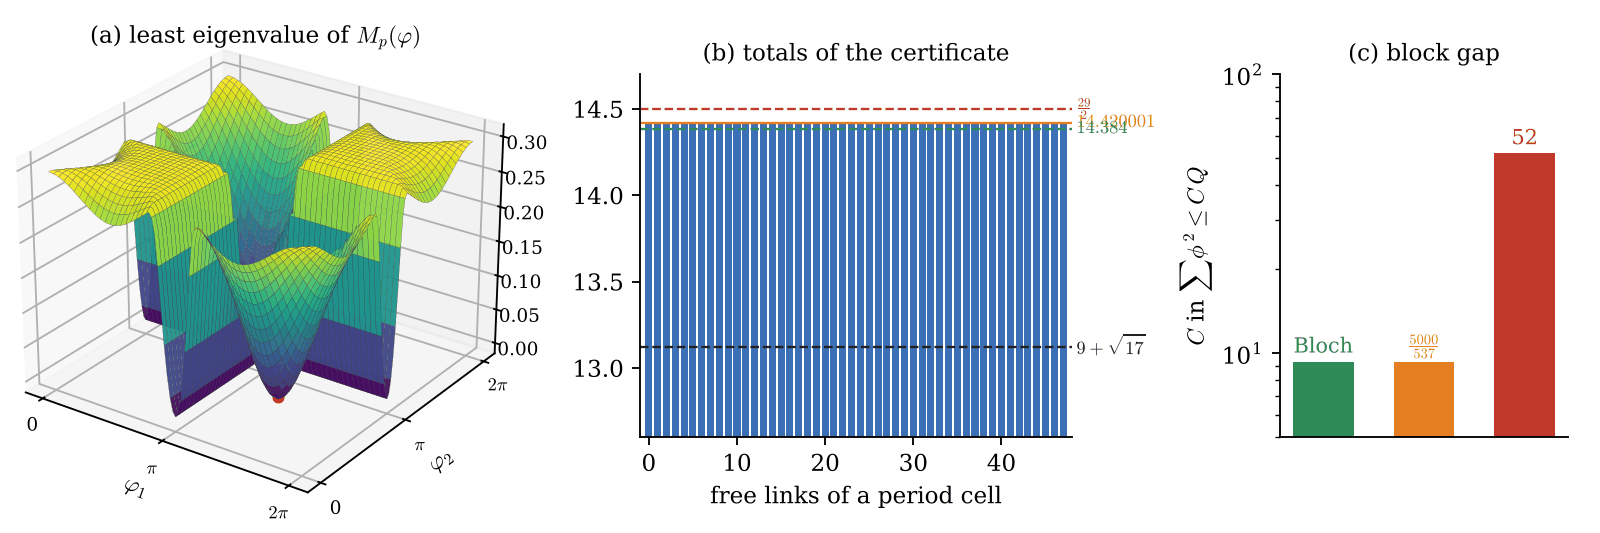
\includegraphics[width=0.95\textwidth]{figures/fig_certificate.png}
\caption{The certificate of Appendix~\ref{app:certificate}. (a)~The least
eigenvalue of $M_p(\varphi)$ over the torus of phases for the plaquette
class with the smallest minimum, about $0.0057$ on a grid of $96^2$ phases
(red dot); Theorem~\ref{thm:certificate} shows it stays positive.
(b)~The forty-eight totals in the definition of $h$, in increasing order,
against $\frac{29}2$, the value $14.420001$ of the largest, the floor
$14.384$ for certificates on the period-two cell, and the lower bound
$9+\sqrt{17}$ for $h_F$. (c)~The constant $C$ in $\sum\phi^2\le CQ$ for the
block gauge: $52$ from Theorem~\ref{thm:blockgap}, $5000/537$ from
Proposition~\ref{prop:blockgapsharp}, and the bulk Bloch value
$1/0.10749=9.3034$, the best constant when $W$ is the set of all
blocks. The eigenvalues in (a) and the Bloch value are in floating point.}
\label{fig:certificate}
\end{figure*}

\begin{theorem}[Computer-assisted]\label{thm:certificate}
For every $N$, every field $Q$ and every $v=(X_eQ_e)$ with $X_e=0$ for
$e\in F$, on $\Z^4$ and on every box,
\[
|\Hess S_0(v,v)|\le14.420001\,|v|^2 .
\]
\end{theorem}

\begin{proof}
We show that every $M_p(\varphi)$ is positive semidefinite, which proves
the theorem by Lemmas~\ref{lem:certificate} and~\ref{lem:certu2}. Write
$z=(1,\cos\varphi_1,\sin\varphi_1,\cos\varphi_2,\sin\varphi_2)$. For each
of the $192$ blocks of size six there is a positive definite integer
symmetric matrix $P$ of size thirty such that
\[
2^{24}\cdot4\cdot10^6\,M(\varphi)_{jk}=\sum_{a,b=0}^4z_az_b\,P_{6a+j,\,6b+k}
\]
for all $j,k$, as polynomials modulo $\cos^2\varphi_a+\sin^2\varphi_a=1$.
For $x\in\R^6$ put $w=z\otimes x$. Then $2^{24}\cdot4\cdot10^6\,x^{\mathsf T}
M(\varphi)x=w^{\mathsf T}Pw$, which is positive for $x\ne0$, since $z_0=1$
gives $w\ne0$. So every block is positive definite at every $\varphi$.
\end{proof}

The proof of Theorem~\ref{thm:certificate} rests on computations of three
kinds. The positivity of the $G_y$, the signs of the weights and the
forty-eight totals are finite statements about rational numbers. The
identities between $M(\varphi)$ and the matrices $P$, and the positive
definiteness of the $P$, are finite statements about integers. All of
these are checked by the Lean~4 kernel in~\cite{Rom26}, on no axioms beyond
\texttt{propext} and \texttt{Quot.sound}; the program there also checks
the positivity at every phase a second time, by interval arithmetic on a
subdivision of the torus of phases. Lemmas~\ref{lem:corners}
to~\ref{lem:certu2} and the formula~\eqref{eq:fp} for the Hessian are the
written proofs above and are not formalised.\footnote{Formalising them
needs matrices over $\C$, the group $\U(N)$ and second derivatives along
geodesics, that is, a library such as Mathlib; the Lean files
of~\cite{Rom26} use only the core library.} We checked the finite data in
exact arithmetic and the positivity at every phase by eigenvalues on an
adaptive grid with a Lipschitz bound, in floating point, and
J.~M.~Lockwood checked it again in exact rational arithmetic with
outward-rounded interval elimination, finding least eigenvalue above
$559/716800$ for every plaquette.

With $14.420001$ in place of $\frac{29}2$ the proofs of
Theorems~\ref{thm:curv} and~\ref{thm:groups} go through unchanged, which
gives the ranges stated in Remark~\ref{rem:hf}. Those theorems are stated
with $\frac{29}2$ because its proof uses no computer.

\def\bibsection{\par\vskip10pt\noindent\hfil\rule{0.5\columnwidth}{0.4pt}\hfil\par\vskip8pt}

\begin{thebibliography}{99}\raggedright\advance\leftskip\labelwidth

\bibitem{AC25}
A.~Adhikari and S.~Cao, Correlation decay for finite lattice gauge theories at weak coupling, Ann. Probab. \textbf{53} (2025), 140--174, \href{https://doi.org/10.1214/24-AOP1702}{doi:10.1214/24-AOP1702}.

\bibitem{Aum44}
G.~Aumann, {\"U}ber R{\"a}ume mit Mittelbildungen, Math. Ann.
\textbf{119} (1944), 210--215,
\href{https://doi.org/10.1007/BF01563741}{doi:10.1007/BF01563741}.

\bibitem{BE85}
D.~Bakry and M.~\'Emery, Diffusions hypercontractives, in \emph{S\'eminaire
de Probabilit\'es XIX}, Lecture Notes in Math. 1123, Springer, Berlin, 1985,
177--206, \href{https://doi.org/10.1007/BFb0075847}{doi:10.1007/BFb0075847}.

\bibitem{BGL14}
D.~Bakry, I.~Gentil and M.~Ledoux, \emph{Analysis and Geometry of Markov
Diffusion Operators}, Grundlehren Math. Wiss. 348, Springer, Cham, 2014,
\href{https://doi.org/10.1007/978-3-319-00227-9}{doi:10.1007/978-3-319-00227-9}.

\bibitem{Bal84a}
T.~Ba{\l}aban, Propagators and renormalization transformations for lattice
gauge theories.~I, Comm. Math. Phys. \textbf{95} (1984), 17--40,
\href{https://doi.org/10.1007/BF01215753}{doi:10.1007/BF01215753}.

\bibitem{Bal85a}
T.~Ba{\l}aban, Averaging operations for lattice gauge theories, Comm. Math.
Phys. \textbf{98} (1985), 17--51,
\href{https://doi.org/10.1007/BF01211042}{doi:10.1007/BF01211042}.

\bibitem{Bal89b}
T.~Ba{\l}aban, Large field renormalization. II. Localization,
exponentiation, and bounds for the $\mathbf R$ operation, Comm. Math. Phys.
\textbf{122} (1989), 355--392,
\href{https://doi.org/10.1007/BF01238433}{doi:10.1007/BF01238433}.

\bibitem{Ban38}
S.~Banach, \"Uber homogene Polynome in $(L^2)$, Studia Math. \textbf{7}
(1938), 36--44,
\href{https://doi.org/10.4064/sm-7-1-36-44}{doi:10.4064/sm-7-1-36-44}.

\bibitem{Bar37}
J.~Barta, Sur la vibration fondamentale d'une membrane, C. R. Acad. Sci. Paris \textbf{204} (1937), 472--473.

\bibitem{BG18}
R.~Basu and S.~Ganguly, $\SO(N)$ lattice gauge theory, planar and beyond, Comm. Pure Appl. Math. \textbf{71} (2018), 2016--2064, \href{https://doi.org/10.1002/cpa.21788}{doi:10.1002/cpa.21788}.

\bibitem{Bha22}
D.~Bhattacharjee, A coherent approach towards quantum gravity, Phys. Sci. Int. J. \textbf{26}(6) (2022), 59--78, \href{https://doi.org/10.9734/psij/2022/v26i6751}{doi:10.9734/psij/2022/v26i6751}.

\bibitem{Bha26}
D.~Bhattacharjee, BLLM: Beyond the LLM with Deep Human-Mind-AI, Zenodo,
release v3.0.5, 2026,
\href{https://doi.org/10.5281/zenodo.23469389}{doi:10.5281/zenodo.23469389}.

\bibitem{Bha26b}
D.~Bhattacharjee, BLLM: Beyond the LLM with Deep Human-Mind-AI, Zenodo,
release v3.1.0, 2026,
\href{https://doi.org/10.5281/zenodo.23484160}{doi:10.5281/zenodo.23484160}.

\bibitem{BB26a}
D.~Bhattacharjee and U.~Bhattacharya, Mass gap of lattice Yang--Mills theory
up to the Dobrushin ceiling, in \emph{Lattice Yang--Mills theory: spacing-uniform
obstructions, the mass gap up to the Dobrushin ceiling, and Lean certificate},
Zenodo, release v2.0.2, 2026,
\href{https://doi.org/10.5281/zenodo.23449466}{doi:10.5281/zenodo.23449466}.

\bibitem{BB26b}
D.~Bhattacharjee and U.~Bhattacharya, Spacing-uniform lattice inequalities
cannot produce the Yang--Mills mass gap, Zenodo, release v1.0.0, 2026,
\href{https://doi.org/10.5281/zenodo.23444339}{doi:10.5281/zenodo.23444339}.

\bibitem{BRS26}
D.~Bhattacharjee, S.~Singha Roy and P.~Samal, Brane-cluster UV completion of quantum gravity, Research Square (2026), \href{https://doi.org/10.21203/rs.3.rs-9053205/v1}{doi:10.21203/rs.3.rs-9053205/v1}.

\bibitem{BSB26}
D.~Bhattacharjee, P.~Samal and S.~Bhattacharya, Geometric structure and
renormalization group flow in chiral Yang--Mills--Higgs theory, Preprints
(2026), \href{https://doi.org/10.20944/preprints202602.2022.v1}
{doi:10.20944/preprints202602.2022.v1}.

\bibitem{BTBS26}
D.~Bhattacharjee, S.~Nath Thakur, S.~Bhattacharya and P.~Samal, $\SU(n)$ holonomy deviations in Calabi--Yau manifolds (CY1--CY4), Preprints (2026), \href{https://doi.org/10.20944/preprints202602.0023.v1}{doi:10.20944/preprints202602.0023.v1}.

\bibitem{BK55}
M.~Biernacki and J.~Krzy\.z, On the monotonity of certain functionals in the theory of analytic functions, Ann. Univ. Mariae Curie-Sk{\l}odowska Sect. A \textbf{9} (1955), 135--147.

\bibitem{Bis09}
M.~Biskup, Reflection positivity and phase transitions in lattice spin
models, in \emph{Methods of Contemporary Mathematical Statistical Physics},
Lecture Notes in Math. 1970, Springer, Berlin, 2009, 1--86,
\href{https://doi.org/10.1007/978-3-540-92796-9_1}{doi:10.1007/978-3-540-92796-9\_1}.

\bibitem{BFS79}
D.~Brydges, J.~Fr\"ohlich and E.~Seiler, On the construction of quantized gauge fields. I. General results, Ann. Physics \textbf{121} (1979), 227--284, \href{https://doi.org/10.1016/0003-4916(79)90098-8}{doi:10.1016/0003-4916(79)90098-8}.

\bibitem{Bum13}
D.~Bump, \emph{Lie Groups}, 2nd ed., Grad. Texts in Math. 225, Springer, New
York, 2013, \href{https://doi.org/10.1007/978-1-4614-8024-2}
{doi:10.1007/978-1-4614-8024-2}.

\bibitem{CNS25}
S.~Cao, R.~Nissim and S.~Sheffield, Expanded regimes of area law for lattice Yang--Mills theories, preprint, 2025, \href{https://arxiv.org/abs/2505.16585}{arXiv:2505.16585}.

\bibitem{Chat19}
S.~Chatterjee, Yang--Mills for probabilists, in \emph{Probability and Analysis in Interacting Physical Systems}, Springer Proc. Math. Stat. 283, Springer, Cham, 2019, 1--16, \href{https://doi.org/10.1007/978-3-030-15338-0_1}{doi:10.1007/978-3-030-15338-0\_1}.

\bibitem{Chat19b}
S.~Chatterjee, Rigorous solution of strongly coupled $\SO(N)$ lattice gauge theory in the large $N$ limit, Comm. Math. Phys. \textbf{366} (2019), 203--268, \href{https://doi.org/10.1007/s00220-019-03353-3}{doi:10.1007/s00220-019-03353-3}.

\bibitem{Cre77}
M.~Creutz, Gauge fixing, the transfer matrix, and confinement on a lattice,
Phys. Rev. D \textbf{15} (1977), 1128--1136,
\href{https://doi.org/10.1103/PhysRevD.15.1128}{doi:10.1103/PhysRevD.15.1128}.

\bibitem{CT73}
J.~M.~Combes and L.~Thomas, Asymptotic behaviour of eigenfunctions for
multiparticle Schr\"odinger operators, Comm. Math. Phys. \textbf{34} (1973),
251--270,
\href{https://doi.org/10.1007/BF01646473}{doi:10.1007/BF01646473}.

\bibitem{Dim13}
J.~Dimock, The renormalization group according to Balaban, I. Small fields, Rev. Math. Phys. \textbf{25} (2013), 1330010, \href{https://doi.org/10.1142/S0129055X13300100}{doi:10.1142/S0129055X13300100}.

\bibitem{Dob68}
R.~L.~Dobrushin, The description of a random field by means of conditional
probabilities and conditions of its regularity, Theory Probab. Appl.
\textbf{13} (1968), 197--224,
\href{https://doi.org/10.1137/1113026}{doi:10.1137/1113026}.

\bibitem{Dob70}
R.~L.~Dobrushin, Prescribing a system of random variables by conditional
distributions, Theory Probab. Appl. \textbf{15} (1970), 458--486,
\href{https://doi.org/10.1137/1115049}{doi:10.1137/1115049}.

\bibitem{DS85}
R.~L.~Dobrushin and S.~B.~Shlosman, Constructive criterion for the uniqueness
of Gibbs field, in \emph{Statistical Physics and Dynamical Systems},
Birkh\"auser, Boston, 1985, 347--370,
\href{https://doi.org/10.1007/978-1-4899-6653-7_20}{doi:10.1007/978-1-4899-6653-7\_20}.

\bibitem{Dri89}
B.~K.~Driver, YM$_2$: continuum expectations, lattice convergence, and lassos, Comm. Math. Phys. \textbf{123} (1989), 575--616, \href{https://doi.org/10.1007/BF01218586}{doi:10.1007/BF01218586}.

\bibitem{Eck54}
B.~Eckmann, R{\"a}ume mit Mittelbildungen, Comment. Math. Helv.
\textbf{28} (1954), 329--340,
\href{https://doi.org/10.1007/BF02566939}{doi:10.1007/BF02566939}.

\bibitem{FH91}
W.~Fulton and J.~Harris, \emph{Representation Theory: A First Course}, Grad.
Texts in Math. 129, Springer, New York, 1991 (reprinted 2004),
\href{https://doi.org/10.1007/978-1-4612-0979-9}{doi:10.1007/978-1-4612-0979-9}.

\bibitem{FILS78}
J.~Fr\"ohlich, R.~Israel, E.~H. Lieb and B.~Simon, Phase transitions and
reflection positivity. I. General theory and long range lattice models,
Comm. Math. Phys. \textbf{62} (1978), 1--34,
\href{https://doi.org/10.1007/BF01940327}{doi:10.1007/BF01940327}.

\bibitem{FS82}
J.~Fr\"ohlich and T.~Spencer, Massless phases and symmetry restoration in abelian gauge theories and spin systems, Comm. Math. Phys. \textbf{83} (1982), 411--454, \href{https://doi.org/10.1007/BF01213610}{doi:10.1007/BF01213610}.

\bibitem{GL10}
C.~Gattringer and C.~B.~Lang, \emph{Quantum Chromodynamics on the Lattice},
Lecture Notes in Phys. 788, Springer, Berlin, 2010,
\href{https://doi.org/10.1007/978-3-642-01850-3}{doi:10.1007/978-3-642-01850-3}.

\bibitem{GBN26}
R.~Ghora, D.~Bhattacharjee, P.~Nandi, P.~Samal, R.~Patra, S.~Singha Roy and S.~Bhattacharya, O'Neill tensor bounds for Riemannian submersions in fibred Calabi--Yau manifolds, Preprints (2026), \href{https://doi.org/10.20944/preprints202602.0125.v1}{doi:10.20944/preprints202602.0125.v1}.

\bibitem{GJ87}
J.~Glimm and A.~Jaffe, \emph{Quantum Physics: A Functional Integral Point
of View}, 2nd ed., Springer, New York, 1987,
\href{https://doi.org/10.1007/978-1-4612-4728-9}{doi:10.1007/978-1-4612-4728-9}.

\bibitem{GKS89}
L.~Gross, C.~King and A.~Sengupta, Two dimensional Yang--Mills theory via stochastic differential equations, Ann. Physics \textbf{194} (1989), 65--112, \href{https://doi.org/10.1016/0003-4916(89)90032-8}{doi:10.1016/0003-4916(89)90032-8}.

\bibitem{Gut80}
A.~H.~Guth, Existence proof of a nonconfining phase in four-dimensional $\U(1)$ lattice gauge theory, Phys. Rev. D \textbf{21} (1980), 2291--2307, \href{https://doi.org/10.1103/PhysRevD.21.2291}{doi:10.1103/PhysRevD.21.2291}.

\bibitem{Hel01}
S.~Helgason, \emph{Differential Geometry, Lie Groups, and Symmetric Spaces},
Grad. Stud. Math. 34, Amer. Math. Soc., Providence, RI, 2001,
\href{https://doi.org/10.1090/gsm/034}{doi:10.1090/gsm/034}.

\bibitem{Hig02}
N.~J.~Higham, \emph{Accuracy and Stability of Numerical Algorithms}, 2nd
ed., SIAM, Philadelphia, 2002,
\href{https://doi.org/10.1137/1.9780898718027}{doi:10.1137/1.9780898718027}.

\bibitem{HS87}
R.~Holley and D.~Stroock, Logarithmic Sobolev inequalities and stochastic
Ising models, J. Stat. Phys. \textbf{46} (1987), 1159--1194,
\href{https://doi.org/10.1007/BF01011161}{doi:10.1007/BF01011161}.

\bibitem{HS94}
B.~Helffer and J.~Sj\"ostrand, On the correlation for Kac-like models in
the convex case, J. Stat. Phys. \textbf{74} (1994), 349--409,
\href{https://doi.org/10.1007/BF02186817}{doi:10.1007/BF02186817}.

\bibitem{Hoe63}
W.~Hoeffding, Probability inequalities for sums of bounded random variables,
J. Amer. Statist. Assoc. \textbf{58} (1963), 13--30,
\href{https://doi.org/10.1080/01621459.1963.10500830}{doi:10.1080/01621459.1963.10500830}.

\bibitem{Hum72}
J.~E.~Humphreys, \emph{Introduction to Lie Algebras and Representation
Theory}, Grad. Texts in Math. 9, Springer, New York, 1972,
\href{https://doi.org/10.1007/978-1-4612-6398-2}{doi:10.1007/978-1-4612-6398-2}.

\bibitem{JW06}
A.~Jaffe and E.~Witten, Quantum Yang--Mills theory, in \emph{The Millennium
Prize Problems}, Clay Mathematics Institute and American Mathematical
Society, Cambridge, MA and Providence, RI, 2006, 129--152,
\url{https://www.claymath.org/wp-content/uploads/2022/06/yangmills.pdf}.

\bibitem{Joh17}
F.~Johansson, Arb: efficient arbitrary-precision midpoint-radius interval
arithmetic, IEEE Trans. Comput. \textbf{66} (2017), 1281--1292,
\href{https://doi.org/10.1109/TC.2017.2690633}{doi:10.1109/TC.2017.2690633}.

\bibitem{Kac90}
V.~G.~Kac, \emph{Infinite-Dimensional Lie Algebras}, 3rd ed., Cambridge University Press, Cambridge, 1990, \href{https://doi.org/10.1017/CBO9780511626234}{doi:10.1017/CBO9780511626234}.

\bibitem{Kal21}
O.~Kallenberg, \emph{Foundations of Modern Probability}, 3rd ed., Springer,
Cham, 2021, \href{https://doi.org/10.1007/978-3-030-61871-1}
{doi:10.1007/978-3-030-61871-1}.

\bibitem{KS75}
J.~Kogut and L.~Susskind, Hamiltonian formulation of Wilson's lattice gauge
theories, Phys. Rev. D \textbf{11} (1975), 395--408,
\href{https://doi.org/10.1103/PhysRevD.11.395}{doi:10.1103/PhysRevD.11.395}.

\bibitem{Lev03}
T.~L\'evy, Yang--Mills measure on compact surfaces, Mem. Amer. Math. Soc. \textbf{166} (2003), no.~790, \href{https://doi.org/10.1090/memo/0790}{doi:10.1090/memo/0790}.

\bibitem{Loc26}
J.~M.~Lockwood, Toward the continuum limit of forest-gauge lattice
Yang--Mills theory: constrained cubes, exact Gaussian diagnostics, and a
gauge-suited mixing test, technical report, 29 October 2026, distributed with
the archive.

\bibitem{Lus77}
M.~L\"uscher, Construction of a selfadjoint, strictly positive transfer matrix
for Euclidean lattice gauge theories, Comm. Math. Phys. \textbf{54} (1977),
283--292,
\href{https://doi.org/10.1007/BF01614090}{doi:10.1007/BF01614090}.

\bibitem{Lus10}
M.~L\"uscher, Properties and uses of the Wilson flow in lattice QCD, J. High
Energy Phys. \textbf{2010}, no.~8, 071,
\href{https://doi.org/10.1007/JHEP08(2010)071}{doi:10.1007/JHEP08(2010)071}.

\bibitem{LW11}
M.~L\"uscher and P.~Weisz, Perturbative analysis of the gradient flow in
non-abelian gauge theories, J. High Energy Phys. \textbf{2011}, no.~2, 051,
\href{https://doi.org/10.1007/JHEP02(2011)051}{doi:10.1007/JHEP02(2011)051}.

\bibitem{MRS93}
J.~Magnen, V.~Rivasseau and R.~S\'en\'eor, Construction of YM$_4$ with an infrared cutoff, Comm. Math. Phys. \textbf{155} (1993), 325--383, \href{https://doi.org/10.1007/BF02097397}{doi:10.1007/BF02097397}.

\bibitem{MJ00}
K.~V.~Mardia and P.~E.~Jupp, \emph{Directional Statistics}, Wiley, Chichester, 2000, \href{https://doi.org/10.1002/9780470316979}{doi:10.1002/9780470316979}.

\bibitem{McS34}
E.~J.~McShane, Extension of range of functions, Bull. Amer. Math. Soc. \textbf{40} (1934), 837--842, \href{https://doi.org/10.1090/S0002-9904-1934-05978-0}{doi:10.1090/S0002-9904-1934-05978-0}.

\bibitem{Mil76}
J.~Milnor, Curvatures of left invariant metrics on Lie groups, Adv.
Math. \textbf{21} (1976), 293--329,
\href{https://doi.org/10.1016/S0001-8708(76)80002-3}{doi:10.1016/S0001-8708(76)80002-3}.

\bibitem{MM94}
I.~Montvay and G.~M\"unster, \emph{Quantum Fields on a Lattice}, Cambridge
University Press, Cambridge, 1994,
\href{https://doi.org/10.1017/CBO9780511470783}{doi:10.1017/CBO9780511470783}.

\bibitem{OS73}
K.~Osterwalder and R.~Schrader, Axioms for Euclidean Green's functions,
Comm. Math. Phys. \textbf{31} (1973), 83--112,
\href{https://doi.org/10.1007/BF01645738}{doi:10.1007/BF01645738}.

\bibitem{OS75}
K.~Osterwalder and R.~Schrader, Axioms for Euclidean Green's functions.~II,
Comm. Math. Phys. \textbf{42} (1975), 281--305,
\href{https://doi.org/10.1007/BF01608978}{doi:10.1007/BF01608978}.

\bibitem{OSei78}
K.~Osterwalder and E.~Seiler, Gauge field theories on a lattice, Ann. Physics
\textbf{110} (1978), 440--471,
\href{https://doi.org/10.1016/0003-4916(78)90039-8}{doi:10.1016/0003-4916(78)90039-8}.

\bibitem{RS80}
M.~Reed and B.~Simon, \emph{Methods of Modern Mathematical Physics I:
Functional Analysis}, revised and enlarged ed., Academic Press, New York,
1980.

\bibitem{Rom26}
T.~Romanov, A proved bound $h_F\le14.420001$ for the four-dimensional
forest-gauge Hessian, computer-assisted certificate with Lean~4 kernel
checks (2026),
\url{https://github.com/romanov360/yang-mills-4d-forest-certificate}.

\bibitem{SBG26}
P.~Samal, D.~Bhattacharjee and R.~Ghora, Renormalization of spacetime dimension, Preprints (2026), \href{https://doi.org/10.20944/preprints202602.0531.v1}{doi:10.20944/preprints202602.0531.v1}.

\bibitem{SS23}
K.~Sakai and S.~Sasaki, Glueball spectroscopy in lattice QCD using gradient
flow, Phys. Rev. D \textbf{107} (2023), 034510,
\href{https://doi.org/10.1103/PhysRevD.107.034510}{doi:10.1103/PhysRevD.107.034510}.

\bibitem{Sei82}
E.~Seiler, \emph{Gauge Theories as a Problem of Constructive Quantum Field
Theory and Statistical Mechanics}, Lecture Notes in Phys. 159, Springer,
Berlin, 1982, \href{https://doi.org/10.1007/3-540-11559-5}{doi:10.1007/3-540-11559-5}.

\bibitem{SZZ23}
H.~Shen, R.~Zhu and X.~Zhu, A stochastic analysis approach to lattice
Yang--Mills at strong coupling, Comm. Math. Phys. \textbf{400} (2023),
805--851, \href{https://doi.org/10.1007/s00220-022-04609-1}{doi:10.1007/s00220-022-04609-1}.

\bibitem{Sla81}
R.~Slansky, Group theory for unified model building, Phys. Rep.
\textbf{79} (1981), 1--128,
\href{https://doi.org/10.1016/0370-1573(81)90092-2}{doi:10.1016/0370-1573(81)90092-2}.

\bibitem{Sta99}
R.~P.~Stanley, \emph{Enumerative Combinatorics, Volume 2}, with an appendix by
S.~Fomin, Cambridge Stud.
Adv. Math. 62, Cambridge University Press, Cambridge, 1999,
\href{https://doi.org/10.1017/CBO9780511609589}{doi:10.1017/CBO9780511609589}.

\bibitem{SW71}
E.~M.~Stein and G.~Weiss, \emph{Introduction to Fourier Analysis on Euclidean Spaces}, Princeton University Press, Princeton, NJ, 1971, \href{https://doi.org/10.1515/9781400883899}{doi:10.1515/9781400883899}.

\bibitem{Uhl82}
K.~K.~Uhlenbeck, Connections with $L^p$ bounds on curvature, Comm. Math.
Phys. \textbf{83} (1982), 31--42,
\href{https://doi.org/10.1007/BF01947069}{doi:10.1007/BF01947069}.

\bibitem{Vil09}
C.~Villani, \emph{Optimal Transport: Old and New}, Grundlehren Math. Wiss.
338, Springer, Berlin, 2009,
\href{https://doi.org/10.1007/978-3-540-71050-9}{doi:10.1007/978-3-540-71050-9}.

\bibitem{Wat44}
G.~N.~Watson, \emph{A Treatise on the Theory of Bessel Functions}, 2nd ed., Cambridge University Press, Cambridge, 1944.

\bibitem{Whi57}
H.~Whitney, \emph{Geometric Integration Theory}, Princeton University
Press, Princeton, 1957,
\href{https://doi.org/10.1515/9781400877577}{doi:10.1515/9781400877577}.

\bibitem{Wil74}
K.~G.~Wilson, Confinement of quarks, Phys. Rev. D \textbf{10} (1974),
2445--2459, \href{https://doi.org/10.1103/PhysRevD.10.2445}{doi:10.1103/PhysRevD.10.2445}.

\end{thebibliography}

\end{document}
